\documentclass[10pt]{memoir}
\setstocksize{220mm}{155mm} 	        
\settrimmedsize{220mm}{155mm}{*}	
\settypeblocksize{170mm}{116mm}{*}	
\setlrmargins{18mm}{*}{*}
\setulmargins{*}{*}{1.2}
%\setlength{\headheight}{5pt}%
\checkandfixthelayout[lines]
\linespread{1.16}
\flushbottom

%%% Hyphenation settings
\usepackage[htt]{hyphenat}
\hyphenation{he-lio-trope opos-sum}
\tracingparagraphs=1
%Hyphenation in Devanāgarī of the edition still missing? Probably this needs to be modified in babel-iast package? 

%%% babel
\usepackage[english]{babel}
\usepackage{babel-iast/babel-iast}

\babelfont[iast]{rm}[Renderer=Harfbuzz, Scale=1.3]{AdishilaSan}%AdishilaSan}
\babelfont[english]{rm}{Adobe Text Pro}

%%% more functionality
\PassOptionsToPackage{hyphens}{url}
\usepackage{hyperref}
\usepackage{pdflscape}
\usepackage{cleveref}
\usepackage{url}
\usepackage{cleveref}
\usepackage{microtype}
\usepackage{lineno}

%\usepackage{bigfoot}
%%% more functions
\usepackage[dvipsnames]{xcolor}
%\usepackage[para,perpage]{footmisc}

%%%für den Counter von Kapiteln und Sätzen! 
\newcommand{\uproman}[1]{\uppercase\expandafter{\romannumeral#1}}
\newcommand{\lowroman}[1]{\romannumeral#1\relax}

\makeindex
\newfontfamily\sanskritfont[Script=Devanagari,Mapping=RomDev,Scale=1.1]{Sanskrit2003}
\usepackage{pifont,fourier-orns,lettrine,psvectorian,paralist,enumitem,pdfpages,wrapfig,tabulary,lettrine,longtable}
\setlist[enumerate]{itemsep=0mm}
\usepackage[autostyle]{csquotes}
\usepackage[defaultlines=2,all]{nowidow}
\usepackage{ellipsis,adforn,booktabs,longtable,url,tikz}
\lineskiplimit=-3pt          

\makechapterstyle{IeT}{%
  \chapterstyle{default}
  \renewcommand*{\printchapternonum}{\centering}
  \renewcommand*{\clearforchapter}{\cleartorecto} 
  \aliaspagestyle{chapter}{empty}}
\chapterstyle{IeT}
\setsecnumdepth{none}  \openright  \nouppercaseheads
\settocdepth{subsubsection}

%%%% test better pagebreaks
%\def\fussy{%
%  \emergencystretch\z@
%  \tolerance 200%
%  \hfuzz .1\p@
%  \vfuzz\hfuzz}

%\interfootnotelinepenalty=10000\relax

%\usepackage[maxfloats=256]{morefloats}

%\maxdeadcycles=500

%raggedbottomsectiontrue
%%\checkandfixthelayout


%%%%%%%  biblatex
%\newcommand{\noun}[1]{\textsc{#1}}    %  philosophy-verbose
\usepackage[backend=biber, sorting=nyt, style=verbose]{biblatex} %%%%ORIGINAL TiE
\renewcommand*{\mkbibnamefamily}[1]{\textsc{#1}}


\DeclareFieldFormat{url}{%
  \mkbibacro{URL}\addcolon\space
  \href{#1}{\nolinkurl{\thefield{urlraw}}}}

\DeclareFieldFormat{citeurl}{%
  \href{#1}{\nolinkurl{\thefield{urlraw}}}} 


\DeclareFieldFormat{postnote}{#1}
\renewcommand{\postnotedelim}{, }
\addbibresource{bindu.bib}

%%% ekdosis
\usepackage[teiexport=tidy,parnotes=true]{ekdosis}% =tidy cleans up HTML and XML documents by fixing markup errors and upgrading legacy code to modern standards. parnotes=footnotes below or above critical apparatus

\SetLineation{lineation=page, modulo} %lineation=page sets thenumbering to start afresh at the top of each page. =modulo makes every fifth line numbered. {lineation=page} makes every line numbered! 

\renewcommand{\linenumberfont}{\selectlanguage{english}\footnotesize} %sets language of lines to English

\SetTEIxmlExport{autopar=false} %autopar=falseinstructs ekdosis to ignore blank lines in the.tex sourcefile as markers for paragraph boundaries. As a result, each paragraph of the edition must be found within an environment associated with the xml <p> element

\SetHooks{
  lemmastyle=\bfseries,
  %refnumstyle=\selectlanguage{english}\bfseries,
  refnumstyle=\selectlanguage{english}\color{blue}\bfseries,
  appheight=0.8\textheight,
}

\newif\ifinapparatus
\DeclareApparatus{source}[
%bhook=\inapparatustrue,
lang=english,
notelang=english,
% bhook=\selectlanguage{english},
bhook=\selectlanguage{english}\textbf{Sources:},%
%maxentries=4, 
%ehook=.]
%sep={] },
%nosep,
]

\newif\ifinapparatus
\DeclareApparatus{testium}[
%bhook=\inapparatustrue,
lang=english,
notelang=english,
% bhook=\selectlanguage{english},
bhook=\selectlanguage{english}\textbf{Testimonia:},
%maxentries=4, 
%ehook=.]
%nosep, 
]

% Declare \ifinapparatus and set \inapparatustrue at the beginning of
% the apparatus criticus block. Also set the language.  
\newif\ifinapparatus
  \DeclareApparatus{default}[
  %bhook=\inapparatustrue, 
  lang=english,
  %maxentries=33,
  %bhook=\selectlanguage{english},
  sep = {] },
  delim=\hskip 0.75em,
  rule=\rule{0.7in}{0.4pt},
]

\newif\ifinapparatus
\DeclareApparatus{philcomm}[
%bhook=\inapparatustrue,
lang=english,
notelang=english,
bhook=\selectlanguage{english}\textbf{Philological Commentary:},
%bhook=\selectlanguage{english},
sep={: },
]

\ekdsetup{
showpagebreaks,
spbmk = \textcolor{blue}{spb},
hpbmk = \textcolor{red}{hpb}
}

%\usepackage{fnpos}
%\makeFNmid
%\makeFNbottom
\usepackage[bottom]{footmisc}
%%%%%%%%%%%%%%%%%%%%%%%%%%%
\makeatletter
\def\blfootnote{\gdef\@thefnmark{}\@footnotetext}
\makeatother
%%%%%%%%%%%%%%%%%%%%%%%%%


% Macros and Definitions for the Print of Sigla
\def\acpc#1#2#3{{#1}\rlap{\textrm{\textsuperscript{#3}}}\textsubscript{\textrm{#2}}\space}
\def\sigl#1#2{{{#1}}\textsubscript{\textrm{#2}}}
\def\None{{\sigl{N}{1}}} \def\Noneac{\acpc{N}{1}{ac}\,} \def\Nonepc{\acpc{N}{1}{pc}\,}
\def\Ntwo{{\sigl{N}{2}}} \def\Noneac{\acpc{N}{2}{ac}\,} \def\Nonepc{\acpc{N}{2}{pc}\,}
\def\Done{{\sigl{D}{1}}} \def\Doneac{\acpc{D}{1}{ac}\,} \def\Donepc{\acpc{D}{1}{pc}\,}
\def\Dtwo{{\sigl{D}{2}}} \def\Dtwoac{\acpc{D}{2}{ac}\,} \def\Dtwopc{\acpc{D}{2}{pc}\,}
\def\Uone{{\sigl{U}{1}}} \def\Uoneac{\acpc{U}{1}{ac}\,} \def\Uonepc{\acpc{U}{1}{pc}\,}                 
\def\Utwo{{\sigl{U}{2}}} \def\Utwoac{\acpc{U}{2}{ac}\,} \def\Utwopc{\acpc{U}{2}{pc}\,}

%%%%%%%%%%%%%% Tattvabinduyoga - List of Witnesses   %%%%%%%%%%%%%%%%%%%
\DeclareWitness{ceteri}{\selectlanguage{english}cett.}{ceteri}[]   
\DeclareWitness{E}{\selectlanguage{english}E}{Printed Edition}[]    
\DeclareWitness{P}{\selectlanguage{english}P}{Pune BORI 664}[]  
\DeclareWitness{B}{\selectlanguage{english}B}{Bodleian 485}[]       
\DeclareWitness{N1}{\selectlanguage{english}N\textsubscript{1}}{NGMPP 38/31}[]
\DeclareWitness{N2}{\selectlanguage{english}N\textsubscript{2}}{NGMPP B 38/35}[]
\DeclareWitness{L}{\selectlanguage{english}L}{LALCHAND 5876}[]  
\DeclareWitness{D}{\selectlanguage{english}D}{IGNCA 30019}[] 
%\DeclareWitness{D2}{\selectlanguage{english}D\textsubscript{2}}{IGNCA 30020}[]  
\DeclareWitness{U1}{\selectlanguage{english}U\textsubscript{1}}{SORI 1574}[] 
\DeclareWitness{U2}{\selectlanguage{english}U\textsubscript{2}}{SORI 6082}[]
%%%%%%%%%%%%%% Tattvabinduyoga - Groups of Witnesses   %%%%%%%%%%%%%%%%%%%
\DeclareWitness{X}{\selectlanguage{english}\alpha}{Alpha Group: D,N1,N2,U1}[]
\DeclareWitness{Y}{\selectlanguage{english}\beta}{Beta Group: B,E,L,P,U2}[]
%%%%%%%%%%%%% Testimonia
\DeclareWitness{Ysv}{\selectlanguage{english}Ysv}{Yogasvarodaya}[] %%%add infos!  

%%%%%%%%%%%%%%%%%%%%%%%%%%%%%%%%%%%%%%%%%%%
% Macro for Editing Abbrevs.
\def\om{\textrm{\footnotesize \textit{om.}\ }} %prints om. for omitted in apparatus
\def\korr{\textrm{\footnotesize \textit{em.}\ }} %prints em. for emended in apparatus
\def\conj{\textrm{\footnotesize \textit{conj.}\ }} %prints conj. for conjectured in apparatus

% \supplied{text} EDITORIAL ADDITION -> Within \lem oder \rdg
% \surplus{text} EDITORIAL DELETION -> Within \lem oder \rdg
% \sic{text} CRUX
% \gap{text} LACUNAE -> [reason=??, unit=??, quantity=??, extent=??]


%%%%%%%%%%%%%%%%%%%%%%%%%%%%%%%%%%%%%%%%%%% All macros of this list can be used in 
% Macro for Editing Abbrevs.
\def\eyeskip{\textrm{{ab.\,oc. }}}
\def\aberratio{\textrm{{ab.\,oc. }}}
\def\ad{\textrm{{ad}}}
\def\add{\textrm{{add.\ }}}
\def\ann{\textrm{{ann.\ }}}
\def\ante{\textrm{{ante }}} 
\def\post{\textrm{{post }}}
%\def\ceteri{cett.\,}                   
\def\codd{\textrm{{codd.\ }}}

\def\coni{\textrm{{coni.\ }}}
\def\contin{\textrm{{contin.\ }}}
\def\corr{\textrm{{corr.\ }}}
\def\del{\textrm{{del.\ }}}
\def\dub{\textrm{{ dub.\ }}}

\def\expl{\textrm{{explic.\ }}} 
\def\explica t{\textrm{{explic.\ }}}
\def\fol{\textrm{{fol.\ }}}
\def\foll{\textrm{{foll.\ }}}
\def\gloss{\textrm{{glossa ad }}}
\def\ins{\textrm{{ins.\ }}}      
\def\inseruit{\textrm{{ins.\ }}} 
\def\im{{\kern-.7pt\lower-1ex\hbox{\textrm{\tiny{\emph{i.m.}}}\kern0pt}}} %\textrm{\scriptsize{i.m.\ }}}      
\def\inmargine{{\kern-.7pt\lower-.7ex\hbox{\textrm{\tiny{\emph{i.m.}}}\kern0pt}}}%\textrm{\scriptsize{i.m.\ }}}      
\def\intextu{{\kern-.7pt\lower-.95ex\hbox{\textrm{\tiny{\emph{i.t.}}}\kern0pt}}}%\textrm{\scriptsize{i.t.\ }}}           
\def\indist{\textrm{{indis.\ }}}  
\def\indis{\textrm{{indis.\ }}}
\def\iteravit{\textrm{{iter.\ }}} 
\def\iter{\textrm{{iter.\ }}}
\def\lectio{\textrm{{lect.\ }}}   
\def\lec{\textrm{{lect.\ }}}
\def\leginequit{\textrm{{l.n. }}} 
\def\legn{\textrm{{l.n. }}}
\def\illeg{\textrm{{l.n. }}}

\def\primman{\textrm{{pr.m.}}}
\def\prob{\textrm{{prob.}}}
\def\rep{\textrm{{repetitio }}}
\def\secundamanu{\textrm{\scriptsize{s.m.}}}            \def\secm{{\kern-.6pt\lower-.91ex\hbox{\textrm{\tiny{\emph{s.m.}}}\kern0pt}}}%   \textrm{\scriptsize{s.m.}}}
\def\sequentia{\textrm{{seq.\,inv.\ }}}  
\def\seqinv{\textrm{{seq.\,inv.\ }}}
\def\order{\textrm{{seq.\,inv.\ }}}
\def\supralineam{{\kern-.7pt\lower-.91ex\hbox{\textrm{\tiny{\emph{s.l.}}}\kern0pt}}} %\textrm{\scriptsize{s.l.}}}
\def\interlineam{{\kern-.7pt\lower-.91ex\hbox{\textrm{\tiny{\emph{s.l.}}}\kern0pt}}}   %\textrm{\scriptsize{s.l.}}}
\def\vl{\textrm{v.l.}}   \def\varlec{\textrm{v.l.}} \def\varialectio{\textrm{v.l.}}
\def\vide{\textrm{{cf.\ }}}
\def\cf{\textrm{{cf.\ }}} 
\def\videtur{\textrm{{vid.\,ut}}}
\def\crux{\textup{[\ldots]} }
\def\cruxx{\textup{[\ldots]}}
\def\unm{\textit{unm.}}
%%%%%%%%%%%%%%%%%%%%%%%%%%%%%%%%%%%%

% List of Scholars
\DeclareScholar{ego}{ego}[
forename=Nils Jacob,
surname=Liersch]

% Persons:14\DeclareScholar{ego}{ego}[15forename=Robert,16surname=Alessi]17% Useful shorthands:18\DeclareShorthand{codd}{codd.}{V,I,R,H}19\DeclareShorthand{edd}{edd.}{Lit,Erm,Sm}20\DeclareShorthand{egoscr}{\emph{scripsi}}{ego}

%Useful shorthands:
%\DeclareShorthand{codd}{codd.}{V,I,R,H}
%\DeclareShorthand{edd}{edd.}{Lit,Erm,Sm}
\DeclareShorthand{egoscr}{em.}{ego}
\DeclareShorthand{egoscrconj}{conj.}{ego}
\DeclareShorthand{egomute}{\unskip}{ego}

\usepackage{xparse}

\NewDocumentEnvironment{tlg}{O{}O{}}{\setlength{\leftskip}{0pt}\vspace{-1ex}\begin{quotation}}{\hfill #1\ \vspace{-1ex}\end{quotation}\vspace{-1ex}} %verse environment
%\NewDocumentEnvironment{tlg}{O{}O{}}{\begin{verse}}{॥#1\hskip-4pt ॥\\ \end{verse}}
\NewDocumentCommand{\tl}{m}{{\selectlanguage{iast} #1}}

\NewDocumentCommand{\extra}{m}{{\textcolor{gray}{#1}}} %command for additions to U2
\NewDocumentCommand{\crazy}{m}{{\textcolor{red}{#1}}} %totally corrupted passage
\NewDocumentCommand{\coro}{m}{{\textcolor{violet}{#1}}} %colour for sentence counter! 

\NewDocumentEnvironment{prose}{O{}}{\begin{otherlanguage}{iast}}{\end{otherlanguage}}
% \NewDocumentEnvironment{padd}{O{}}{\begin{otherlanguage}{iast}}{\end{otherlanguage}}
\NewDocumentEnvironment{tlate}{O{}}
%\NewDocumentEnvironment{tadd}{O{}}

%Define two commands: \skp ("sanskrit plus"), to be ignored by TeX in
%the edition text, but processed in the TEI output. Conversely, \skm
%("sanskrit minus") is to be processed in the edition text, but
%ignored if found in the apparatus criticus and in the TEI output:

\NewDocumentCommand{\skp}{m}{}
\TeXtoTEIPat{\skp {#1}}{#1}

%\NewDocumentCommand{\skpp}{m}{}
%\TeXtoTEIPat{\skpp {#1}}{#1}

\NewDocumentCommand{\skm}{m}{\unless\ifinapparatus#1-\fi}
\TeXtoTEIPat{\skm {#1}}{}

% \NewDocumentCommand{\dd}{}{/\hskip-4pt/}
\NewDocumentCommand{\dd}{}{\mbox{/\hskip-4pt/}}
\TeXtoTEIPat{\dd {}}{//}


%%% modify environments and commands
%%% TEI mapping
\TeXtoTEIPat{\begin {tlg}}{<lg>} %lg=(Group of verse (s)) contains one or more verses or lines of verse that together form a formal unit (e.g. stanza, chorus).
\TeXtoTEIPat{\end {tlg}}{</lg>}

\TeXtoTEIPat{\begin {prose}}{<p>}
\TeXtoTEIPat{\end {prose}}{</p>}

\TeXtoTEIPat{\begin {tlate}}{<p>}
\TeXtoTEIPat{\end {tlate}}{</p>}

\TeXtoTEIPat{\\}{}
\TeXtoTEIPat{\linebreak}{<br/>}
\TeXtoTEIPat{\noindent}{}
%\TeXtoTEI{tl}{l}
\TeXtoTEI{emph}{hi}
\TeXtoTEI{bigskip}{}
\TeXtoTEI{None}{N1}
\TeXtoTEI{Ntwo}{N2}
\TeXtoTEI{Done}{D1}
\TeXtoTEI{Dtwo}{D2}
\TeXtoTEI{Uone}{U1}
\TeXtoTEI{Utwo}{U2}
%\TeXtoTEIPat{/}{ |}
%\TeXtoTEI{//}{ ||}
\TeXtoTEIPat{\korr}{em. }
\TeXtoTEIPat{\conj}{conj.}
\TeXtoTEIPat{\om}{om.}
\TeXtoTEIPat{english}{}
\TeXtoTEIPat{\hskip}{}
\TeXtoTEIPat{\hskip-4pt}{}
\TeXtoTEIPat{\hskip-2pt}{}
\TeXtoTEIPat{-}{ }
\TeXtoTEIPat{4pt}{}
\TeXtoTEIPat{2pt}{}
\TeXtoTEIPat{\textcolor {#1}{#2}}{<hi rend="#1">#2</hi>} 

% Nullify \selectlanguage in TEI as it has been used in
% \DeclareWitness but should be ignored in TEI.
\TeXtoTEI{selectlanguage}{}



\FormatDiv{1}{\begin{center}\Large}{\end{center}}
\FormatDiv{2}{\begin{center}\small}{\end{center}}
\FormatDiv{3}{\bfseries}{.}
\title{Yogatattvabindu of Rāmacandra\\ A Critical Edition and Annotated Translation together with a Comparative Analysis of the \\Complex Early Modern Yoga Yaxonomies}
\date{\today}

\parindent=15pt
\begin{document}

%Zitiermöglichkeiten:
%\footcite[See][p.\,1]{goldstein01:_tibet_englis_diction_moder_tibet}
%\footnote{\cite{goldstein01:_tibet_englis_diction_moder_tibet}.}

\frontmatter
\thispagestyle{empty}
\begin{center}
  {\Large \emph{The Yogatattvabindu}}\\[3mm]
\end{center}



\newpage

\

\thispagestyle{empty}



\normalsize


\newpage


\begin{center}
\thispagestyle{empty}

\

\vskip 2mm

\begin{otherlanguage}{iast}
\LARGE \sanskritfont{Yogatattvabindu}
\end{otherlanguage}

\vskip .4cm

\Huge Yogatattvabindu \\[7mm]
\Large Critical Edition\\
and annotated Translation\\
together with a Comparative Analysis of the \\Complex Early Modern Yoga Yaxonomies 


\large

\vspace{3cm}

By

Nils Jacob Liersch
\small
\vfill

\vfill

Indica et Tibetica Verlag \\ % $\cdot$ 
Marburg 2024

\vskip 6mm

\end{center}

\newpage
\newpage \ \thispagestyle{empty}
\small  \

\noindent

\
\vfill


\small
\noindent \textbf{Bibliographische Information Der Deutschen Bibliothek}

\noindent
Die Deutsche Bibliothek verzeichnet diese Publikation in der Deutschen Nationalbibliographie;
detaillierte bibliographische Informationen sind im Internet über http://dnb.ddb.de abrufbar.

\noindent
\textbf{Bibliographic information published by Die Deutschen Bibliothek}

\noindent
Die Deutsche Bibliothek lists this publication in the Deutsche Nationalbibliographie; detailed
bibliographic data is available in the Internet at http://dnb.ddb.de.  


\vskip 1cm

\noindent
\copyright\ Indica et Tibetica Verlag, Marburg 2024

\medskip

\noindent
Alle Rechte vorbehalten / All rights reserved

\medskip

\noindent
Ohne ausdrückliche Genehmigung des Verlages ist es nicht gestattet, das Werk oder einzelne Teile
daraus nachzudrucken, zu vervielfältigen oder auf Datenträger zu speichern.

\smallskip

\noindent
Apart from any fair dealing for the purpose of private study, research, criticism or review, no
part of this book may be reproduced or translated in any form, by print, photo form, microfilm, or
any other means without written permission. Enquiries should be made to the publishers.

\bigskip

\noindent
Satz: \ \ Nils Jacob Liersch \\
Herstellung: \ \ BoD – Books on Demand GmbH, Norderstedt  \\

\bigskip

\noindent
%\ISBN     

\normalsize

\newpage

%\maketitle
\clearpage
\tableofcontents
\addtocounter{page}{-1}
\thispagestyle{empty}
\clearpage


\mainmatter

\chapter{Conventions in the Critical Apparatus}
\section{Sigla in the Critical Apparatus}

\begin{itemize}
\item E : Printed Edition
\item P : Pune BORI 664
\item L : Lalchand Research Library LRL5876
\item B : Bodleian Oxford D 4587
‚\item \None : NGMPP B 38-31
\item \Ntwo : NGMPP B 38-35 / A 1327-14
\item \Done : IGNCA 30019
\item \Uone : SORI 1574
\item \Utwo : SORI 6082
\end{itemize}

\chapter{Critical Edition \& Annotated Translation}
\cleardoublepage
  \begin{alignment}[
  texts=edition[class="edition"];
  translation[class="translation"],
  ]
  \begin{edition}
    \begin{prose}[p41_03]
      \noindent
%-----------------------------
%puruṣasya nṛtyadarśanāt gītaśravaṇāt/ vallabhavastuno  darśanāt/ yaḥ ānanda utpadyate saḥ svargalokaḥ               kathyate/ rogapīḍito durjanebhyaḥ puruṣasya yat duḥkham utpadyate   tadbahutaraṃ  narakaṃ kathyate// \E
%puruṣasya nṛtyadarśanāt gītaśravaṇāt  vallabhavastuno  darśanāt  ya  ānanda utpadyate     svargalokaḥ               kathyate  rogapīḍato durjjanebhya puruṣasya yaduḥkham   utpadyate   tadbahutaraṃ  narakaṃ kathyate \P
%puruṣasya nityadarśanāt gītaśravaṇāt/ vallabhavastuno  darśanāt/ yaḥ ānanda utpadyate     svargalokaḥ               kathyate  rogapīḍato durjanebhya  puruṣasya yat duḥkha  utpadyate// tadbahutaraṃ  narakaṃ kathyate// \B
%puruṣasya nityadarśanāt gītaśravaṇāt  vallabhavastuno  darśanāt  yaḥ ānanda utpadyate     svargalokaḥ               kathyate  rogapīḍano durjanebhya  puruṣasya yad duḥkhaṃ utpadyate// tadbahutaraṃ  narakaṃ kathyate// \L
%puruṣasya nṛtyadarśanād gītaśravaṇāt  vallabhavastuno  darśanāt  yaḥ ānanda utpadyate sa bahurānaṃdaḥ svargaphulaḥ? kathyate/ rogapīḍādurjanebhyaḥ puruṣasya duḥkhaṃ     utpadyate// tat bahutaraṃ nakaṃ   kathyate/ \D
%puruṣasyāvādya   nṛtyodgītaśravaṇād  vallabhavasttuno  darśanād  yā  ānanda utpadyate sa bahurānaṃdaḥ svargaphalaḥ? kathyate  rogapīḍa   durjanebhyaḥ puruṣasya duḥkham     utpadyate       bahutaraṃ narakaṃ kathyate \U1
%puruṣasya darśanāt//   gītaśravaṇāt// vallabhavastuno  darśanāt//    ānanda utpadyate sa svargaloka                 kathyate//rogapīḍāto durjanebhyaḥ puruṣasya duḥkha      utpadyate    tadbahutaraṃ narakaṃ kathyate// \U2
%\om                                                                 \N1
%\om                                                                 \N2
%-----------------------------
%By witnessing the dance, by listening to songs, and by looking at beloved objects, one attains supreme bliss, which is called heaven. The suffering experienced by a person afflicted by disease and tormented by wicked individuals is considered a lesser hell.   
%-----------------------------
\note[type=source, labelb=303, labele=_303e, nosep]{cf. YSv (PT pp. 843-844): samagradarśanān muktaḥ svargabhogañ ca matsukham | tad etac cintayā yāti rogaśokavivarjjitaḥ |}
\note[type=source, labelb=304, labele=_303e, nosep]{cf. SSP 3.14 (Ed. pp. 59-60): yat sukhaṃ tat svargaḥ | yad duḥkhaṃ tan narakaḥ | yat karma tad bandhanaṃ | yo nirvikalpaḥ sā muktiḥ | svasvarūpajñānadaśāyāṃ nidrādau svātmajāgaraḥ śāntir bhavati | evaṃ sarvadeheṣu viśvarūpaḥ parameśvaraḥ paramātmā 'khaṇḍasvabhāvena ghaṭe ghaṭe cit svarūpī tiṣṭhati |}
\app{\lem[wit={ceteri}]{puruṣasya}
  \rdg[wit={U1}]{puruṣasyāvādya}}
\app{\lem[wit={D,E,P}]{nṛtyadarśanāt}/ 
  \rdg[wit={D}]{nityadarśanād}
  \rdg[wit={U2}]{darśanāt ||}
  \rdg[wit={U1}]{nṛtyod°}}
\app{\lem[wit={ceteri}]{gītaśravaṇāt}
  \rdg[wit={U1}]{gītaśravaṇād}}/ 
 vallabhavastuno
\app{\lem[wit={U1}]{darśanāt}
  \rdg[wit={U1}]{darśanād}}/ 
\app{\lem[wit={P}]{ya}
  \rdg[wit={U1}]{yā}
  \rdg[wit={B,D,E,L}]{yaḥ}
  \rdg[wit={U2}]{\om}}
ānanda utpadyate
\app{\lem[wit={E}]{saḥ}
  \rdg[wit={D,U1,U2}]{sa}}
\app{\lem[wit={B,E,L,P}, alt={svargalokaḥ}]{svargalo:\\kaḥ}
  \rdg[wit={U2}]{svargaloka}
  \rdg[wit={D}]{bahurānaṃdaḥ svargaphulaḥ}
  \rdg[wit={U1}]{bahurānaṃdaḥ svargaphalaḥ}}
kathyate/
roga\app{\lem[wit={D},alt={°pīḍā°}]{pīḍā}
  \rdg[wit={U1}]{°pīḍa°}
  \rdg[wit={E}]{°pīḍito}
  \rdg[wit={B,P}]{°pīḍato}
  \rdg[wit={U2}]{°pīḍāto}
  \rdg[wit={L}]{°pīḍano}
}\app{\lem[wit={ceteri}]{durjanebhyaḥ}
  \rdg[wit={B,L,P}]{durjanebhya}}
puruṣasya
\app{\lem[wit={L}, alt={yad duḥkhaṃ}]{yad\skp{-}duḥkhaṃ}
  \rdg[wit={E}]{yat duḥkham}
  \rdg[wit={B}]{yat duḥkha}
  \rdg[wit={P}]{yaduḥkham}
  \rdg[wit={D,U1}]{duḥkhaṃ}
  \rdg[wit={U2}]{duḥkha}}
utpadyate/
\app{\lem[wit={ceteri}]{tad\skp{-}bahutaraṃ}
  \rdg[wit={D}]{tat bahutaraṃ}
  \rdg[wit={U1}]{bahutaraṃ}}
\app{\lem[wit={ceteri}]{narakaṃ}
  \rdg[wit={U1}]{nakaṃ}}
kathyate/\linelabel{_303e}
%-------------------
%                                                                                                      atha ca yatkarmakaraṇāt manomadhye śaṃkā na bhavati    tatkarma muktikāraṇam/ \E
%                                                                                                      atha ca yatkarmakaraṇān manomadhye śaṃkā na bhavati    tatkarma muktikāraṇam   \P %%%7662.jpg 
%                                                                                                      atha ca yatkarmakaraṇāt manobudhye śaṃkā na bhavati    tatkarma kamuktikāraṇam// \B
%                                                                                                      atha ca yatkarmakaraṇāt manobudhye śaṃkā na bhavati    tatkarma kamuktikāraṇam// \L
%                                                                                                     \om                                                                 \N1
%                                                                                                      atha ca yatkarmakaraṇāt manomadhye śaṃkā na bhaviti    tatkarma muktikāraṇaṃ// \D
%                                                                                                     \om                                                                  \N2
%atha ca yatkarmakaraṇāt sarveṣāṃ lokānāṃ svamanasī ca śubhaṃ na bharate tatkarma baṃdhanam ity ucyate atha ca yatkarmakaraṇāt manomadhye śaṃkā na bhavati    tatkarma muktikāraṇam \U1
%                                                                                                      atha ca yatkarmakaraṇān manomadhye śakā  na bhavaṃti// tatkarma muktikāraṇaṃ// \U2
%-----------------------------
%Furthermore, through the performance of actions in which the minds of all beings and one's own mind do not fill with auspiciousness, those actions are said to be the bondage of karma. And thus, when there are no doubts in the mind regarding the performance of actions, those actions become the cause of liberation.
%----------------------------
\note[type=source, labelb=305, labele=_305e, nosep]{cf. YSv (PT p. 844): yatkarmā karmaṇā śaṅkā manomadhye bhaved vahiḥ | tatkarmakaraṇaṃ muktir ity āha bhagavān śivaḥ |}
\app{\lem[wit={U1}, alt={atha ca yat karmakaraṇāt sarveṣāṃ lokānāṃ svamanasi ca śubhaṃ na bharate tat karma bandhanam ity ucyate}]{atha ca yatkarmakaraṇāt sarveṣāṃ lokānāṃ svamanasi ca śubhaṃ na bharate tatkarma bandhanam-ity-ucyate}
  \rdg[wit={ceteri}]{\om}}/
atha ca \app{\lem[wit={P,U2},alt={yatkarmakaraṇān}]{yat:\\karmakaraṇā\skp{n-ma}}
  \rdg[wit={ceteri}]{yatkarmakaraṇāt}
}\app{\lem[wit={ceteri},alt={manomadhye}]{\skm{n-ma}nomadhye}
  \rdg[wit={B,L}]{manobudhye}} 
\app{\lem[wit={ceteri}]{śaṅkā}
  \rdg[wit={U2}]{śakā}}
na
\app{\lem[wit={ceteri}]{bhavati}
  \rdg[wit={U2}]{bhavaṃti}}
tatkarma
\app{\lem[wit={ceteri}]{muktikāraṇam}
  \rdg[wit={L,B}]{kamuktikāraṇam}}/\linelabel{_305e}
\end{prose}
\ekddiv{
  head={[\uproman{42}. \textbf{rājayogaśarīre cihnāni}]},
  type=section,
  depth=2, 
  n=XLII 
}
\xmlhead[h42]{XLII. rājayogaśarīre cihnāni]}
\label{attributesrajabody}
\begin{prose}[p42_01]
  \noindent
%----------------------------
%idānīṃ rājayogāc charīre    yādṛśāni cihnāni bhavanti   tāni kathyante// \E
%idānī  rogayogācharīre     etādṛśāni cihnāni bhavaṃti   tāni kathyaṃte   \P
%idānī  rājayogāc charīre// etādṛśāni cihnāni bhavaṃti// tāni kathyaṃte// \B 7170.jpg end 7171.jpg beginning
%idānīṃ rājayogāc charīre   etādṛśāni cihnāni bhavaṃti   tāni kathyaṃte// \L
%\om                                                                     \N1
%idānīṃ rājayogāc charīre   etādṛśāni cihnāni bhavaṃti// tāni kathyaṃte// \D
%\om                                                                     \N2
%idānīṃ rājayogācharīre     etādṛśāni cihnāni bhavaṃti   tāni kathyaṃte   \U1
%idānī  rājayogāśarīre      etādṛśāni cihnāni bhavaṃti// tāni kathyaṃte// \U2
%-----------------------------
%Now, such attributes arise in the body from Rājayoga. These are taught [in the following]. 
%-----------------------------
\app{\lem[wit={ceteri}]{idānīṃ}
  \rdg[wit={B,P,U2}]{idānī}}
\app{\lem[wit={D,E,L}]{rājayogāc\skp{-}charīre}
  \rdg[wit={B}]{rājayogāc charīre ||}
  \rdg[wit={U1}]{rājayogācharīre}
  \rdg[wit={U2}]{rājayogāśarīre}
  \rdg[wit={P}]{rogayogācharīre}}
\app{\lem[wit={ceteri}]{etādṛśāni}
  \rdg[wit={E}]{yādṛśāni}}
cihnāni bhavanti/ tāni kathyante/
%-----------------------------
%sakalaroganāśaḥ   sakalapṛthvīṃ   paśyati/  tad anaṃtaraṃ              jñānam utpadyate// \E [p.55]
%sakalaroganāśaḥ   sakalāṃ pṛthvīṃ paśyati   tad aṃtaraṃ                jñānam utpadyate   \P
%sakalaroganāśaḥ   sakalapṛthvīṃ   paśyatī/  tad anaṃtaraṃ              jñānam utpadyate// \B
%sakalaroganāśaḥ   sakalapṛthvīṃ   paśyati/  tad anaṃtaraṃ              jñānam utpadyate// \L
%\om                                                                                       \N1
%sakalaroganāśaḥ   sakalapṛthvīṃ   paśyatī/  tad anaṃtaraṃ tatvaviṣayaṃ jñānam utpadyate/  \D %%%p. 15 verso 
%\om                                                                                       \N2
%sakalarogaḥ nāśaḥ sakalapṛthvīṃ   paśyati   tad anaṃtaraṃ tatvaviṣayaṃ jñānam utpadyate   \U1
%sakalaroganāśaḥ   sakalapṛthvīṃ   paśyati// tad anaṃtara---------------jñānam utpadyate// \U2
%-----------------------------
%All diseases are destroyed. He sees the entire earth. Then (tad anaṃtaraṃ) knowledge in the realm of reality is generated.   
%-----------------------------
\note[type=source, labelb=_308, labele=_308e, nosep]{cf. YSv (PT p. 844): yasya darśanamātreṇa rogaśokavivarjitaḥ | paramānandacittaḥ syāt tapasvī caiva kīrttitaḥ | saptadvīpā bhaved dṛṣṭā tattvajñānaṃ tato bhavet | sarvabhāvaṃ vijānīyād vajradeho bhavet tathā | sarpadaṣṭe viṣaṃ na syāt kṣudhā nidrā tṛṣā tathā |}
\app{\lem[wit={ceteri}]{sakalaroganāśaḥ}
  \rdg[wit={U1}]{sakalarogaḥ nāśaḥ}}/\linelabel{_308}
\app{\lem[wit={ceteri}, alt={sakalapṛthvīṃ}]{sakala:\\pṛthvīṃ}
  \rdg[wit={P}]{sakalāṃ pṛthvīṃ}}
paśyati/
\app{\lem[wit={ceteri}]{tad\skp{-}anantaraṃ}
  \rdg[wit={P}]{tad aṃtaraṃ}
  \rdg[wit={U2}]{tad anaṃtara°}}
\app{\lem[wit={D,U1}]{tattvaviṣayaṃ}
  \rdg[wit={ceteri}]{\om}}
jñānam-utpadyate/
%-----------------------------
%samagrā  bhāṣā  jānāti/  tataḥ puruṣasya deho vajramayo bhavati/  sarpadaṃśena    maraṇaṃ na bhavati/   \E
%samagrāṃ bhāṣāṃ jānāti   tataḥ puruṣasya deho vajramayo bhavati   sarpadaṃśo      maraṇaṃ na bhavati    \P
%samagrā  bhāṣa  jānāti   tataḥ puruṣasya deho vajramayo bhavati// sarpadaṃśema    maraṇaṃ na bhavatī/   \B
%samagra  bhāṣā    jānāti tataḥ puruṣasya deho vajramayo bhavati// sarpadaṃśe      maraṇaṃ    bhavati//  \L
%\om                                                                                                     \N1
%samagrāṃ bhāṣāṃ jānāti/  tataḥ puruṣasya deho vajramayo bhavati/  sarpadaṃśe satī maraṇaṃ na bhavati/   \D
%\om                                                                                                     \N2
%samagrāṃ bhāṣāṃ jānāti   tataḥ puruṣasya deho vajramayo bhavati   sarpadaṃśe satī maraṇaṃ na bhavati    \U1
%samagrā bhāṣā   jānāti// tataḥ puruṣasya deho vajramayo bhavati// sarpadaṃśe      maraṇaṃ na vati//     \U2
%-----------------------------
%He realizes the totality of language. Because of that [Rājayoga?] the body of the human becomes indestructable. Death through a snake-bite does not arise. 
%-----------------------------
\app{\lem[wit={P,D,U1}]{samagrāṃ bhāṣāṃ}
  \rdg[wit={E,U2}]{samagrā bhāṣā}
  \rdg[wit={B}]{samagrā bhāṣa}
  \rdg[wit={L}]{samagra bhāṣā}}
jānāti/
tataḥ puruṣasya deho vajramayo bhavati/ 
sarpa\app{\lem[wit={D,L,U1,U2}, alt={°daṃśe}]{daṃśe}
  \rdg[wit={P}]{°daṃśo}
  \rdg[wit={E}]{°daṃśena}
  \rdg[wit={B}]{°daṃśema}}
\app{\lem[type=emendation, resp=egoscr]{sati}
  \rdg[wit={D,U1}]{satī}
  \rdg[wit={ceteri}]{\om}}
maraṇaṃ
\app{\lem[wit={ceteri}]{na}
  \rdg[wit={L}]{\om}}
\app{\lem[wit={ceteri}]{bhavati}
  \rdg[wit={B}]{bhavatī}
  \rdg[wit={U2}]{vati}}/
%-----------------------------
%tataḥ puruṣasya bubhukṣā--pipāsā--nidrollatā------śītoṣṇatā bādhāṃ na kurvanti/ \E
%tataḥ puruṣasya bunnukṣā--pipāsā--nidrolmatā------śītatā----bādhā na kurvaṃti \P
%tatpuruṣasya    babhukṣā--pipāsā--nidrollatā------śīta------bādhā na kurvanti/ \B
%tatpuruṣasya    babhukṣā--pipāsā--nidroṣṇatā------śīta------bādhā na kurvanti... \L
%\om                                                                 \N1
%tataḥ puruṣasya bubhukṣā--pipāsā--nidrā/ uṣṇatā// śīta nā   bādhāṃ na kuroti???/ \D
%\om                                                                 \N2
% \om                                                         \U1
%tataḥ puruṣasya bubhukṣā--pipāsā--nidroṣṭṇatā-----śīta------bādhāṃ na kurvaṃti// \U2
%-----------------------------
%Then the afflictions of hunger, thirst, sleepiness, and heat do not arise for the person. 
%-----------------------------
\app{\lem[wit={ceteri}]{tataḥ}
  \rdg[wit={B,L}]{tat°}
  \rdg[wit={U1}]{\om}}
\app{\lem[wit={ceteri}]{puruṣasya}
  \rdg[wit={U1}]{\om}}
\app{\lem[wit={E,D,U2}]{bubhukṣā}
  \rdg[wit={P}]{bunnukṣā}
  \rdg[wit={B,L}]{babhukṣā}
  \rdg[wit={U1}]{\om}
}\app{\lem[wit={L},alt={pipāsanidroṣṇatā°}]{pipāsanidroṣṇatā}
  \rdg[wit={U2}]{pipāsanidroṣṭṇatā°}
  \rdg[wit={D}]{pipāsanidrā | uṣṇatā ||}
  \rdg[wit={E,B}]{pipāsanidrollatā}
  \rdg[wit={P}]{pipāsanidrolmatā}
  \rdg[wit={U1}]{\om}
}\app{\lem[wit={ceteri},alt={°śīta°}]{śīta}
  \rdg[wit={P}]{śītatā}
  \rdg[wit={E}]{śītoṣṇatā}
  \rdg[wit={D}]{śīta nā}
  \rdg[wit={U1}]{\om}
}\app{\lem[wit={P,B,L}]{bādhā na}
  \rdg[wit={E,D,U2}]{bādhāṃ na}
  \rdg[wit={U1}]{\om}}
\app{\lem[wit={ceteri}]{kurvanti}
  \rdg[wit={D}]{kuroti}
  \rdg[wit={U1}]{\om}}/
\linelabel{_308e}
    \end{prose}
  \end{edition}
  \begin{translation}
    \begin{tlate}[p41_03]
      \noindent
The person's bliss that is generated as a result of seeing dance, listening to songs, [and] viewing beloved objects, that [bliss] is called heaven. The person's suffering that arises as a result of the pain caused by disease, and wicked people, that great [suffering] is called hell. Moreover, an action that does not bring goodness to all people and one's mind, that action is said to be bondage.\footnote{This sentence is only preserved in \getsiglum{U1} (\getsiglum{N1} and \getsiglum{N2} have a \textit{lacunae} here and the other manuscript of the \alpha-group omits the sentence, too). Nevertheless, this sentence significantly improves the meaning of the entire paragraph. Therefore, it is likely that the sentence belongs to the original text. This error in the other witnesses can easily be explained here as a haplography of the following sentence, as they begin similarly. A similar statement is found in Rāmacandra's source text, the \emph{Siddhasiddhāntapaddhati} (cf. sources).} And also, the action that does not create fear in the mind that action is the cause of liberation.\footnote{Structurally, lacking any introductory statement, these sentences at first sight do not convincingly align with the context of the yogic body's contents. However, the structure is consistently preserved across all witnesses. Furthermore, this sequence corresponds to the presentation of contents in the \emph{Siddhasiddhāntapaddhati}, as well as the \emph{Yogasvarodaya} (cf. sources). Both source texts conclude the chapter with information about the contents of the yogic body. Rāmacandra's formulations are a synthesis of the two source texts. \citeauthor{ssplonavla} (Ed. p. 60, cf. sources) notes the following regarding the corresponding passage in the \emph{Siddhasiddhāntapaddhati}: ``Thus, the Supreme Lord of universal nature exists in every manifestation in the form of \textit{cit}. Heaven and hell are not two worlds which the souls visit after leaving the body, but only mental states of happiness or sorrow.''}
\end{tlate}
\ekddiv{
  head={[\uproman{42}. \textbf{Characteristics of rājayogic body}]},
  type=section,
  depth=2, 
  n=XLII.1 
}
\xmlhead[h42]{[XLII. Characteristics of rājayogic body]}
\label{attributesrajabody}
\begin{tlate}[p42_01]
  \indent
Now, such characteristics manifest in the body through Rājayoga.\footnote{The repeated mention of the effects of Rājayoga seems redundant since the topic has been covered extensively already in section \uproman{16}-\uproman{17}. Nevertheless, these specific results have not been mentioned so far. In the descriptions of previous chapters, the unhinderedness, equanimity and bliss resulting from Rājayoga were emphasized. Here, the focus shifts to physical results such as health, strength, supernatural abilities or resilience.} They are described. The eradication of all diseases occurs. He sees the entire world. Subsequently, knowledge whose range is the principles arises. He understands all languages. Then, the person's body becomes as hard as a diamond. After a snake bite has taken place, death does not occur. Then, the troubles of hunger, thirst, sleep, heat and cold do not arise for the person.
\flushpage 
    \end{tlate}
  \end{translation}
\end{alignment}
\pagebreak %after pp. 99-100
%%%%%%%%%%%%%%%%%%%%%%%%%%%%%%%%%%%%%%%%%%
%%%%%%%%%%%%%%%%%%%%%%%%%%%%%%%%%%%%%%%%%% 
%%%%%%%%PAGEBREAK%%%%%%%PAGEBREAK%%%%%%%%%
%%%%%%%%%%%%%%%%%%%%%%%%%%%%%%%%%%%%%%%%%% 
%%%%%%%%%%%%%%%%PAGEBREAK%%%%%%%%%%%%%%%%%
%%%%%%%%%%%%%%%%%%%%%%%%%%%%%%%%%%%%%%%%%% 
%%%%%%%%PAGEBREAK%%%%%%%PAGEBREAK%%%%%%%%%
%%%%%%%%%%%%%%%%%%%%%%%%%%%%%%%%%%%%%%%%%% 
%%%%%%%%%%%%%%%%%%%%%%%%%%%%%%%%%%%%%%%%%% 
%%%%%%%%%%%%%%%%%%%%%%%%%%%%%%%%%%%%%%%%%% 
%%%%%%%%%%%%%%%%%%%%%%%%%%%%%%%%%%%%%%%%%% 
%%%%%%%%PAGEBREAK%%%%%%%PAGEBREAK%%%%%%%%%
%%%%%%%%%%%%%%%%%%%%%%%%%%%%%%%%%%%%%%%%%% 
%%%%%%%%%%%%%%%%PAGEBREAK%%%%%%%%%%%%%%%%%
%%%%%%%%%%%%%%%%%%%%%%%%%%%%%%%%%%%%%%%%%% 
%%%%%%%%PAGEBREAK%%%%%%%PAGEBREAK%%%%%%%%%
%%%%%%%%%%%%%%%%%%%%%%%%%%%%%%%%%%%%%%%%%% 
%%%%%%%%%%%%%%%%%%%%%%%%%%%%%%%%%%%%%%%%%% 
%%%%%%%%%%%%%%%%%%%%%%%%%%%%%%%%%%%%%%%%%% 
%%%%%%%%%%%%%%%%%%%%%%%%%%%%%%%%%%%%%%%%%% 
%%%%%%%%PAGEBREAK%%%%%%%PAGEBREAK%%%%%%%%%
%%%%%%%%%%%%%%%%%%%%%%%%%%%%%%%%%%%%%%%%%% 
%%%%%%%%%%%%%%%%PAGEBREAK%%%%%%%%%%%%%%%%%
%%%%%%%%%%%%%%%%%%%%%%%%%%%%%%%%%%%%%%%%%% 
%%%%%%%%PAGEBREAK%%%%%%%PAGEBREAK%%%%%%%%%
%%%%%%%%%%%%%%%%%%%%%%%%%%%%%%%%%%%%%%%%%% 
%%%%%%%%%%%%%%%%%%%%%%%%%%%%%%%%%%%%%%%%%%
\begin{alignment}[
  texts=edition[class="edition"];
  translation[class="translation"],
  ]
  \begin{edition}
    \begin{prose}[p42_02]
      \noindent
%-----------------------------
%vāksiddhir bhavati/  vidyatpāte           kācidbādhāpi na bhavati// \E
%vāksiddhir bhavati                                        \P
%vāksiddhir bhavatī/  vidyutpāte           kācidglānir na bhavati// \B
%vāksiddhir bhavati/  vidyutpāte           kācidglānir na bhavati// \L
%\om                                                                 \N1
%vāksiddhir bhavati/  vidyutpāte śarīre    na kiṃcid glānir bhavati/ \D
%\om                                                                 \N2
%                     vidyutpāte śarīre    kvācid glānir na bhavati  \U1
%vāksiddhir bhavati// vidyutpāte           kācid  dhānir na bhavati// \U2
%-----------------------------
%Perfection of speech arises. Within the moment of a thunderstroke any kind of fatigue does not arise in the body.  
%-----------------------------
\note[type=source, labelb=_308, labele=_308e, nosep]{cf. YSv (PT p. 844): uṣṇatā śītatā ceti vāksiddhiḥ syān na saṃśayaḥ | vidyutpāte 'pi dehasya kvacid dhānir na jāyate |}\linelabel{_308}
vāksiddhir-bhavati/ vidyutpāte
    \app{\lem[wit={D,U1}]{śarīre}
      \rdg[wit={ceteri}]{\om}}
    \app{\lem[wit={U1},alt={kvācid glānir na}]{kvācid-glānir-na}
      \rdg[wit={B,L}]{kācid glānir na}
      \rdg[wit={D}]{na kiṃcid glānir}
      \rdg[wit={E}]{kācidbādhāpi}
      \rdg[wit={U2}]{kācid dhānir na}}
    bhavati/\linelabel{_308e}
%-----------------------------
%tadanaṃtaraṃ  pavanarūṣī puruṣī bhavati/  samagrāṃ pṛthvīṃ dṛṣṭyā paśyati/   aṇimādyaṣṭasiddhir bhavati/ \E
%tadanaṃtaraṃ  pavanarūpī puruṣo bhavati   samagrāṃ pṛthvīṃ dṛṣṭyā paśyati    aṇimādyaṣṭasiddhir bhavati  \P
%tadanaṃtara   pavanarūpi puruṣo bhavati// samagrāṃ pṛthvī  dṛṣṭā paśyati/    aṇimādyāṣṭasiddhir bhavati/ \B scribe switches so much between i and ī
%tadanaṃtaraṃ  pavanarūpi puruṣo bhavati// samagrāṃ pṛthvīṃ dṛṣṭā paśyati//   aṇimādyāṣṭasiddhir bhavati// \L
%\om                                                                 \N1
%tadanaṃtaraṃ  pavanayopī puruṣo bhavati   samagrāṃ pṛthvīṃ dṛṣṭyā paśyati/   aṇimādyaṣṭasiddhir bhavati//  \D
%\om                                                                 \N2
%tadanaṃtaraṃ  pavanayogī puruṣo bhavati   samagrāṃ pṛthvīṃ dṛṣṭvā paśyati    aṇimādyāṣṭasiddhir bhavati  \U1 %%%291.jpg
%tadanaṃtaraṃ  pavanarūpī puruṣo bhavati// samagrāṃ pṛthvīṃ dṛṣṭvā paśyati//  aṇimāmahimāgarimāladhimā tathā prātikāmyamīśatvaṃ// viśītvaṃ// ity āṣṭasiddhayaḥ////  \U2
%-----------------------------
%Subsequently, the person becomes like the wind. He sees the entire earth with a glance. The eight supernatural powers arise.  
%-----------------------------
\note[type=source, labelb=_309, labele=_309e, nosep]{cf. YS (PT p. 844): tato 'sau vāyuyogī syād dṛṣṭvā pṛthvīkulānvitaḥ | aṇimādyaṣṭasiddhiḥ syān mahāpadmodayas tathā | āgacchanti samīpe ca nidhayo nātra saṃśayaḥ |}\linelabel{_309}
tadanantaraṃ
    pavana\app{\lem[wit={P,U2}, alt={°rūpī}]{rūpī}
      \rdg[wit={B,L}]{°rūpi}
      \rdg[wit={U1}]{°yogī}
      \rdg[wit={D}]{°yopī}
      \rdg[wit={E}]{°rūṣī}}
    \app{\lem[wit={ceteri}]{puruṣo}
      \rdg[wit={E}]{puruṣī}} bhavati/
    samagrāṃ
    \app{\lem[wit={ceteri}]{pṛthvīṃ}
      \rdg[wit={B}]{pṛthvī}}
    \app{\lem[wit={D,E,P}]{dṛṣṭyā}
      \rdg[wit={B,L}]{dṛṣṭā}
      \rdg[wit={U1,U2}]{dṛṣṭvā}} paśyati/
    \app{\lem[wit={ceteri},alt={aṇimādyaṣṭasiddhir}]{aṇimādyaṣṭasiddhi\skp{r-bha}}
      \rdg[wit={U2}]{aṇimāmahimāgarimāladhimā tathā}
    }\app{\lem[wit={ceteri},alt={bhavati}]{\skm{r-bha}vati}
      \rdg[wit={U2}]{ prātikāmyamīśatvaṃ || viśītvaṃ || ity āṣṭasiddhayaḥ ||}}/ \linelabel{_309e}
  \end{prose}\\
%-----------------------------
%                                                                                                               mahāpadmādyā nava nidhyayaḥ samīpa āgacchanti/ \E
%śrīpadmaś ca mahāpadmaḥ saṃkho makarakachapa       kuṃdonukuṃda------nīlaś ca vijñeyā nidhayo nava-------------mamahāpadmā  dhānavanidhaya samīpe āgachaṃti \P     %%%7663.jpg 
%śrīpadmaś ca mahāpadmaṃ śaṃkho makarakacchapaḥ//   kuṃdonukuṃdoś  ca nīlaś-ca vajrayonī cīdātmakā// śrīnamaḥ   mahāpadmājñā navinidhyayaḥ//samipe āgacchatī//  nava nidhayaḥ samīpa āgacchanti/ \B
%śrīpadmaś ca mahāpadmaṃ śaṃkho makarakachapaḥ//    kuṃdonukuṃdoś  ca nīlaś ca vajrayonī cidātmakā// śrīnamaḥ   mahāpadmājñā nanidhyayaḥ//  samipe āgacchaṃti// -------------\om-------- \L
%                                                                                                               mahāpadmādyā nidhyayaḥ      samīpe āgacchaṃti// \D
%                                                                                                               mahāpadmādyā nava nidhapa   samīpe āgacchaṃti \U1
%   padmaś ca mahāpadmaś ca śaṃkho makarakachapaḥ// mukuṃdo kuṃdaś ca nīlaś ca vajrayo navanidhi//etādṛśaṃ                                  samīpe āgacchati// \U2 %%%421.jpg
%\om \N1
% \om \N2
%mahāpadmaśca padmaśca śaṅkho makarakacchapau | mukundakunda- nīlāśca kharvaśca nidhayo nava ---> Wisdomlib quote 
% -----------------------------
% 1. Padma (lotus) and 2. Mahāpadma (great lotus), 3. Śaṃkha (conch), 4. Makara (crocodile), 5. Kacchapa (turtle), 6. Mukunda (gem), 7. Kunda (jasmine), 8. Nīla (saphire) und 9. Kharva (another gem) are the nine treasures.
%
%The nine treasures beginning with the mahāpadma etc. approach nearby.  
%-----------------------------
  \note[type=source, labelb=_309x, labele=_309xe, nosep]{ =  \citetitle{amaraed} 1.1.165-1.1.166: mahāpadmāś ca padmaś ca śaṅkho makarakacchapau | mukundakundanīlāś ca kharvaś ca nidhayo nava ||}
\linelabel{_309x}
  \begin{tlg}[42_1]
    \noindent
 \tl{\extra{\app{\lem[type=emendation, resp=egoscr, alt={mahāpadmaś ca padmaś ca}]{mahāpadmaś-ca padmaś-ca}
    \rdg[wit={U2}]{padmaś ca mahāpadmaś ca}
    \rdg[wit={P,B}]{śrīpadmaś ca mahāpadmaṃ}
    \rdg[wit={D,E,L,U1}]{\om}}
\app{\lem[wit={B,L,U2}]{śaṅkho}
  \rdg[wit={P}]{saṃkho}
  \rdg[wit={D,U1}]{\om}}
\app{\lem[type=emendation, resp=egoscr]{makarakacchapau}
  \rdg[wit={B,L,U2}]{makarakachapaḥ}
  \rdg[wit={P}]{makarakachapa°}
  \rdg[wit={D,U1}]{\om}}}/}\\
\tl{\extra{\app{\lem[type=emendation, resp=egoscr,alt={mukundakundanīlāś ca}]{mukundakundanīlāś-ca}
  \rdg[wit={U2}]{mukuṃdo kuṃdaś ca nīlaś ca}
  \rdg[wit={P}]{kuṃdonukuṃdanīlaś ca}
  \rdg[wit={B,L}]{kuṃdonukuṃdoś ca nīlaś ca}
\rdg[wit={D,U1}]{\om}}
\app{\lem[type=emendation, resp=egoscr,alt={kharvaś ca nidhayo nava}]{kharvaś-ca nidhayo nava}
  \rdg[wit={P}]{vijñeyāni dhayonava}
  \rdg[wit={B,L}]{vajrayonī cīdātmakā}
  \rdg[wit={U2}]{vajrayo navanidhi}
  \rdg[wit={D,U1}]{\om}}\dd{}\begin{otherlanguage}{english}\uproman{42}.1\end{otherlanguage}\hskip-2pt\dd{}}}\\
\end{tlg}
\begin{prose}[p42_03]
  \app{\lem[wit={E,D,U1}]{mahāpadmādyā}
     \rdg[wit={B,L}]{mahāpadmājñā}
  \rdg[wit={P}]{mamahāpadmā}}
\app{\lem[wit={E}]{nava nidhyayaḥ}
  \rdg[wit={U1}]{nava nidhapa}
  \rdg[wit={D}]{nidhyayaḥ}
  \rdg[wit={L}]{nanidhyayaḥ ||}
  \rdg[wit={B}]{navinidhyayaḥ ||}
  \rdg[wit={P}]{dhānavanidhaya}}
\app{\lem[wit={E}]{samīpa}
  \rdg[wit={ceteri}]{samīpe}}
\app{\lem[wit={ceteri}]{āgacchanti}
  \rdg[wit={U2}]{āgacchati}
  \rdg[wit={B}]{āgacchatī ||  nava nidhayaḥ samīpa āgacchanti |}}/\linelabel{_309e}\linelabel{_309xe}
%-----------------------------
%ākāśamadhye daśasu dikṣu        gamanāgamane bhavataḥ balaṃ bhavati/                                                                                     parameśvaraṃ samīpe paśyati/   karaṇe  haraṇe sāmarthyaṃ    bhavati// \E [P.56]
%ākāśamadhye daśasu dikṣu        gamanāgamanabalaṃ           bhavati       yatra loke gamanechā bhavati     tatra loke gacchati  ajñā sarvatra sphurati   parameśvaraṃ samīpe paśyati    karaṇe  haraṇe sāmarthyaṃ    bhavati \P
%ākāśamadhye daśasu dikṣu        gamanāgamanavallabhaṃ       bhavati//     yatra loke gamanechā bhavati/    yatra loke gacchati/ ajñā sarvatra sphurati// parameśvaraṃ samīpe paśyaṃtī/  karaṇe  haraṇe sāmarthyaṃ    bhavati// \B
%ākāśamadhye daśasu dikṣu        gamanāgamanavallabhaṃ       bhavati//     yatra loke gamanechā bhavati//  yatra loke gacchati// ajñā sarvatra sphurati   parameśvaraṃ samīpe paśyati    karaṇe  haraṇe sāmarthyaṃ    bhavati// \L%0028.jpg
%ākāśamadhye daśasu dikṣumadhye  gaṃmanāgamanabalaṃ          bhavatī/      yatra lo.. gamanechā bhavati    tatra loke gacchati/  ājñā sarvatra sphurati// parameśvaraṃ samīpe paśyati/   karaṇaṃ haraṇe .. ..marthyaṃ bhavati// \D
%ākāśa-------daśasu dikṣumadhye  gamanāgamanabalaṃ           bhavati       yatra loke gamanechā bhavatī    yatra loke gacchati   ājñā sarvatra sphurati   parameśvaraṃ samīpe paśyati    karaṇe  haraṇe ca sāmarthyaṃ bhavati \U1
%ākāśamadhye daśa   dikṣu        gamanāgamanabalam           bhavati//     yatra loke gamanechā bhavati//  tatra loke gacchati// ajñā sarvatra sphurati// parameśvaraṃ samipe paśyaṃti// karaṇe  taraṇe sāmarthyaṃ    bhavati// \U2
%\om                                                                 \N1
%\om                                                                 \N2
%-----------------------------
%Within the ten cardinal points in space the power over death and rebirth arises. Wherever there is a desires to go in the world, one goes there. Ignorance disappears everywhere. One sees the Supreme Lord nearby. There is the capability of accomplishing tasks and removing obstacles.
%-----------------------------
\note[type=source, labelb=_311, labele=_311e, nosep]{cf. YSv (PT p. 844): yatrecchā gamanaṃ tatra svarge marttye rasātale | sphuraty ājñākhyaḥ sarvatra samīpe parameśvaraḥ | kāraṇe hāraṇe śakto rakṣaṇe 'pi ca pārvati | ātmamadhye mano nityaṃ nirjane nivaset sudhīḥ | kṛtvātmamanasor aikyaṃ prāpnoti paramaṃ padam |}
\linelabel{_311}
\app{\lem[wit={ceteri}]{ākāśamadhye}
  \rdg[wit={U1}]{ākāśa°}}
\app{\lem[wit={ceteri}]{daśasu}
  \rdg[wit={U2}]{°daśa}}
\app{\lem[wit={ceteri}]{dikṣu}
  \rdg[wit={D,U1}]{dikṣumadhye}}
\app{\lem[wit={D,P,U1,U2}]{gamanāgamanabalaṃ}
  \rdg[wit={B,L}]{gamanāgamanavallabhaṃ}
  \rdg[wit={E}]{gamanāgamane bhavataḥ balaṃ}}
\app{\lem[wit={ceteri}]{bhavati}
  \rdg[wit={B}]{bhavatī}}/
yatra loke gamanechā
\app{\lem[wit={ceteri}]{bhavati}
  \rdg[wit={U1}]{bhavatī}}/
\app{\lem[wit={ceteri}]{tatra}
  \rdg[wit={B,P,U1}]{yatra}}
loke gacchati/
ajñā sarvatra sphurati/
parameśvaraṃ samīpe
\app{\lem[wit={ceteri}]{paśyati}
  \rdg[wit={B,U2}]{paśyaṃti}}/
\app{\lem[wit={ceteri}]{karaṇe}
  \rdg[wit={D}]{karaṇaṃ}}
\app{\lem[wit={ceteri}]{haraṇe}
  \rdg[wit={U2}]{taraṇe}}
\app{\lem[wit={ceteri}]{sāmarthyaṃ}
  \rdg[wit={U1}]{ca sāmarthyaṃ}
  \rdg[wit={D}]{....marthyaṃ}}
bhavati/
\linelabel{_311e}
\end{prose}
  \end{edition}
  \begin{translation}
    \begin{tlate}[p42_02]
      \noindent
        Perfection of speech arises. Within the moment of a thunderstrike, fatigue does not occur in the body at any time. Subsequently, the person assumes the nature of the wind. He sees the entire earth with a glance. The eight supernatural powers beginning with ``becoming infinitely small'' etc. (\textit{aṇimādi}) arise.
    \end{tlate}
    \begin{tlate}[42_1]
      \extra{\paragraph{\uproman{42}.1 } 1. Mahāpadma (``great lotus'') 2. Padma (``lotus''), 3. Śaṃkha (``conch''), 4. Makara (``crocodile''), 5. Kacchapa (``turtle''), 6. Mukunda (``gem''), 7. Kunda (``jasmine''), 8. Nīla (``saphire'') and 9. Kharva (``[another type of] gem'') are the nine treasures.}\footnote{The verse is absent in the \alpha-group and therefore greyscaled. These so-called nine treasures of god Kubera are mentioned, i.e. in \textit{Śivapurāṇa} 2.3.15. I emendend the edition according to the traditional list. The nine treasures that an virtuous emperor possesses are also mentioned in \citetitle{sarvangayoga} 3.21 (\textit{jākaiṃ saba baiṭhe hī sūjñai} | \textit{asa sabahiṃna kī bhāṣā būjñai} | \textit{sakala siddhi ājñā mahiṃ jākai} | \textit{navanidhi sadā rahaiṃ ḍhiṃga tākai} || 21 ||) as one of the result of Rājayoga (Rājayoga in the \citetitle{sarvangayoga} is \textit{vajrolīmudrā}). Furthermore, they are mentioned in \citetitle{jogpradipyaka} 601 (\textit{nāṭika chaṃda sahajahī pāvai aṣṭasidha navanidha cali āvai} | \textit{prāṇāyāma ādi vasi hoī dasavai dvāra pahautai soī} || 601 ||) in the context of the so-called \textit{mahābandhamudrā}. Furthermore, the \textit{navanidhi}s occur in the \textit{vajrolī-section} of the \textit{Jog Manjarī}: \textit{jākauṃ saba dehī ko sūjhai aura sakala jīva kī bhāṣā būjhai} | \textit{sarva siddhi āgyā maiṃ jākai navanidhi rahai sadā ḍhiṃga tākai} |}
    \end{tlate}
    \begin{tlate}[p42_03]
     \\\\ \indent The nine treasures, beginning with the Mahāpadma, approach nearby. The power over death and rebirth arises within the ten cardinal points in space. Wherever one desires to go in the world, one goes there. Ignorance disappears everywhere. One sees the Supreme Lord nearby. The capability to create and destroy arises.
      \flushpage
    \end{tlate}
  \end{translation}
\end{alignment}
\pagebreak %after pp. 101-102
%%%%%%%%%%%%%%%%%%%%%%%%%%%%%%%%%%%%%%%%%%
%%%%%%%%%%%%%%%%%%%%%%%%%%%%%%%%%%%%%%%%%% 
%%%%%%%%PAGEBREAK%%%%%%%PAGEBREAK%%%%%%%%%
%%%%%%%%%%%%%%%%%%%%%%%%%%%%%%%%%%%%%%%%%% 
%%%%%%%%%%%%%%%%PAGEBREAK%%%%%%%%%%%%%%%%%
%%%%%%%%%%%%%%%%%%%%%%%%%%%%%%%%%%%%%%%%%% 
%%%%%%%%PAGEBREAK%%%%%%%PAGEBREAK%%%%%%%%%
%%%%%%%%%%%%%%%%%%%%%%%%%%%%%%%%%%%%%%%%%% 
%%%%%%%%%%%%%%%%%%%%%%%%%%%%%%%%%%%%%%%%%% 
%%%%%%%%%%%%%%%%%%%%%%%%%%%%%%%%%%%%%%%%%% 
%%%%%%%%%%%%%%%%%%%%%%%%%%%%%%%%%%%%%%%%%% 
%%%%%%%%PAGEBREAK%%%%%%%PAGEBREAK%%%%%%%%%
%%%%%%%%%%%%%%%%%%%%%%%%%%%%%%%%%%%%%%%%%% 
%%%%%%%%%%%%%%%%PAGEBREAK%%%%%%%%%%%%%%%%%
%%%%%%%%%%%%%%%%%%%%%%%%%%%%%%%%%%%%%%%%%% 
%%%%%%%%PAGEBREAK%%%%%%%PAGEBREAK%%%%%%%%%
%%%%%%%%%%%%%%%%%%%%%%%%%%%%%%%%%%%%%%%%%% 
%%%%%%%%%%%%%%%%%%%%%%%%%%%%%%%%%%%%%%%%%% 
%%%%%%%%%%%%%%%%%%%%%%%%%%%%%%%%%%%%%%%%%% 
%%%%%%%%%%%%%%%%%%%%%%%%%%%%%%%%%%%%%%%%%% 
%%%%%%%%PAGEBREAK%%%%%%%PAGEBREAK%%%%%%%%%
%%%%%%%%%%%%%%%%%%%%%%%%%%%%%%%%%%%%%%%%%% 
%%%%%%%%%%%%%%%%PAGEBREAK%%%%%%%%%%%%%%%%%
%%%%%%%%%%%%%%%%%%%%%%%%%%%%%%%%%%%%%%%%%% 
%%%%%%%%PAGEBREAK%%%%%%%PAGEBREAK%%%%%%%%%
%%%%%%%%%%%%%%%%%%%%%%%%%%%%%%%%%%%%%%%%%% 
%%%%%%%%%%%%%%%%%%%%%%%%%%%%%%%%%%%%%%%%%%
\begin{alignment}[
  texts=edition[class="edition"];
  translation[class="translation"],
  ]
  \begin{edition}
    \ekddiv{
      head={[\uproman{43}. \textbf{gurubhakteḥ phalam}]},
      type=section,
      depth=2, 
      n=XLIII
    }
    \xmlhead[h43]{[XLIII. gurubhakteḥ phalam]}
    \begin{prose}[p43_01]
\noindent      
%-----------------------------
%idaṃ gurubhakteḥ phalaṃ            ātmamadhye manaso viśrāma--karaṇamicchatā      puruṣeṇa sadguroḥ sevāṃ kṛtvā   sāvadhānaṃ manaḥ karaṇīyam/        abhyāsabalāt paramaprāptiḥ/  \E
%idaṃ gurubhaktaiḥ phalaṃ           ātmamadhye manaso viśrāma--karaṇamichatā       puruṣeṇa sadguroḥ sevāṃ kṛtvā   sāvadhānaṃ manaḥ karaṇīyaṃ         abhyāsabalāt paramaprāptiḥ \P
%idaṃ gurubhakteḥ  phalaṃ//         ātmamadhye manaso viśrāmaṃ karaṃṇaṃmicchatāṃ// puruṣeṇa sadguroḥ sevāṃ kṛtvā   sāvadhānaṃ manaḥ kṛtvā karaṇīyam// abhyāsabalāt paramaprāptiḥ//\B
%idaṃ gurubhakteḥ  phalaṃ//         ātmamadhye manaso viśrāmaṃ karaṇam icchatāṃ//  puruṣeṇa sadguroḥ sevāṃ kṛtvā   sāvadhānaṃ manaḥ kṛtvā karaṇīyaṃ...abhyāsabalāt// paramaprāptiḥ// \L
%idaṃ gurubhakteḥ  phalaṃ           ātmamadhye manaso viśrāma--karaṇam icchatā     puruṣeṇa sadguruḥ sevāṃ kṛ..    sāvadhānaṃ manaḥ karaṇīyaṃ/        abhyāsabalāt paramaprāptiḥ/\D
%idaṃ gurubhakteḥ  phalaṃ           ātmamadhye manaso viśrāma--karaṇam icchatā     puruṣeṇa sadguruḥ sevāṃ kṛtvā   sāvadhānaṃ manaḥ karaṇīyaṃ         abhyāsabalāt paramaprāptiḥ\U1
%idaṃ gurubhakteḥ  phalaṃ bhavati// ātmamadhye manaso viśrāme  karaṇam ichatā      puruṣeṇa sadguroḥ sevāṃ kṛtvā// māvadhānaṃ manaḥ karaṇīyaṃ//       abhyāsabalāt paramapadaprāptiḥ\U2
%\om                                                                 \N1
%\om                                                                 \N2
%-----------------------------
%This is the result of devotion to the teacher. Within the self resides the mind's longing for inner peace. The individual who has served the teacher should nurture an attentive mind. Through the power of practice, one attains the highest state.
%-----------------------------
idaṃ
\app{\lem[wit={ceteri}]{gurubhakteḥ}
  \rdg[wit={P}]{gurubhaktaiḥ}}
\app{\lem[wit={ceteri}]{phalaṃ}
  \rdg[wit={U2}]{phalaṃ bhavati}}/
ātmamadhye manaso
\app{\lem[wit={ceteri},alt={viśrāmakaraṇam}]{viśrāmakaraṇa\skp{m-i}}
  \rdg[wit={B}]{viśrāmaṃ karaṃṇaṃm}
  \rdg[wit={L}]{viśrāmaṃ karaṇam}
}\app{\lem[wit={ceteri},alt={icchatā}]{\skm{m-i}cchatā}
  \rdg[wit={B,L}]{icchatāṃ}}/
puruṣeṇa
\app{\lem[wit={ceteri}]{sadguroḥ}
  \rdg[wit={D,U1}]{sadguruḥ}} 
sevāṃ
\app{\lem[wit={ceteri}]{kṛtvā}
  \rdg[wit={D}]{kṛ..}
  \rdg[wit={U2}]{kṛtvā ||}}
\app{\lem[wit={ceteri}]{sāvadhānaṃ}
  \rdg[wit={U2}]{māvadhānaṃ}}
manaḥ
\app{\lem[wit={ceteri}]{karaṇīyam}
  \rdg[wit={L}]{kṛtvā karaṇīyaṃ}
  \rdg[wit={B}]{kṛtvā karaṇīyam}}/ 
\app{\lem[wit={ceteri}, alt={abhyāsabalāt}]{abhyāsabalā\skp{t-pa}}
  \rdg[wit={L}]{abhyāsabalāt ||}
}\app{\lem[wit={ceteri}, alt={paramaprāptiḥ}]{\skm{t-pa}ramaprāptiḥ}
  \rdg[wit={U2}]{paramapadaprāptiḥ}}/\\
%-----------------------------
% tena      svaśiṣyamanasaḥ  svāsthyaṃ   karttavyam/  candrasūryyau yāvat piṃḍe  niścalau bhavataḥ//  \E %[p.57]
% tena      svasya manasaḥ   samarasyaṃ  karttavyam   caṃdrasūryau  yāvat piṃḍo  niścalo  bhavati     \P
% tena      svasya manasaḥ                                                                            \B %stemma point?! omission?!
% tena      svasya manasaḥ   samarasaṃ   karttavyaṃ   caṃdrasūrya---yāt   piṃḍo  niścalo  bhavati//   \L
% tena saha svasya manaḥ     samarasyaṃ  karttavyaṃ/  caṃdrasūryau  yāvit piṃde  niścalau bhavatiḥ//  \D
% tena saha svascha manaḥ                karttavyaṃ   caṃdrasūryau  yāvat piṃdau niścalo  bhavati     \U1
% tena      svasya manasaḥ   samarasyaṃ  karttavyaṃ// caṃdrasūrya---vat   piṃḍo  niścalo  bhavati//   \U2  %%%421verso.jpg
% \om                                                                \N1
%\om                                                                 \N2
%-----------------------------
%Through this, one should harmonize one's own mind. Just as the sun and the moon remain unchanging, an unchanging body emerges.
%----------------------------
\note[type=source, labelb=_312, nosep]{cf. YSv (PT p. 844): candraḥ sūryaḥ sthiro yāvat tāvad dehasthitis tathā | tāvad ekaṃ samābhāṣya prāpnoti ca sadāgatiḥ | sa bhavet kavitā dhīrā niścalā śāntir eva ca | gurupādaprasādena tad aikyaṃ yāti siddhibhāk |}\linelabel{_312}
\app{\lem[wit={ceteri}]{tena}
  \rdg[wit={D,U1}]{tena saha}}
\app{\lem[wit={B,L,P,U2}]{svasya manasaḥ}
  \rdg[wit={D}]{svasya manaḥ}
  \rdg[wit={U1}]{svascha manaḥ}
  \rdg[wit={E}]{svaśiṣyamanasaḥ}}
\app{\lem[wit={L}]{samarasaṃ}
  \rdg[wit={D,P,U2}]{samarasyaṃ}
  \rdg[wit={E}]{svāsthyaṃ}
  \rdg[wit={B,U1}]{\om}}
\app{\lem[wit={D,L,U1,U2}]{kartavayaṃ} 
  \rdg[wit={E,P}]{kartavyam}
  \rdg[wit={B}]{\om}}
\app{\lem[wit={E,P,U1}, alt={candrasūryau yāvat}]{candrasūryau yāva\skp{t-pi}}
  \rdg[wit={D}]{caṃdrasūryau yāvit}
  \rdg[wit={L}]{caṃdrasūryayāt}
  \rdg[wit={U2}]{caṃdrasūryavat}
  \rdg[wit={B}]{\om}
}\app{\lem[wit={D,E}, alt={piṇḍe}]{\skm{t-pi}ṇḍe}
  \rdg[wit={P,L,U2}]{piṇḍo}
  \rdg[wit={U1}]{piṃḍau}
  \rdg[wit={B}]{\om}}
\app{\lem[wit={D,E}]{niścalau}
  \rdg[wit={P,L,U1,U2}]{niścalo}
  \rdg[wit={B}]{\om}}
\app{\lem[wit={E}]{bhavataḥ}
  \rdg[wit={D}]{bhavatiḥ}
  \rdg[wit={P,L,U1,U2}]{bhavati}}/
%A disciple enjoying the state of samvitkriyā, vikaraṇodaya, cidvilāsa and vishranti, becomes enlightened on his own. Those who are favourite to guru indeed enjoy merger with the Absolute, when pada and piṇḍa are identified on dissolution of one's mental activities. 
%----------------------------
%          samyak---svabhāva-kiraṇodaya---cidvilāsa--grastaṃ        svaśāṃti samatāṃ  svayam eva yāti/ \E %[p.57]
%          samyak---svabhāva-kiraṇodaya---cidvilāsa--grastaṃ        svaśāṃti manasā   svayam eva yāmi \P
%                                     samaradvilāsa//grastaṃ        svaśāṃti manasā   svam   eva śāṃti// \B %stemma point?! omission?!
% śloka    samyak---svabhāva-kiraṇodaya---cidvilāsa  grastaṃ        svaśāṃti manasā   svayam eva śāṃti... \L
% ślokaḥ// samyak---svabhāva-kiraṇodaya---cidvilāsaṃ/grastaṃ        svaśāṃti mavatāṃ  svayam eva yāti/ \D
% śloka    samyagaḥ svabhāva-kiraṇodaya---cidvilāsaṃ grastasamagraṃ saśāṃti  mahatāṃ  svayam eva yāti \U1
% ślokaḥ// samyak---svabhāva-karaṇotdṛdi--cidvilāsa--grastaṃ        svaśāṃti bhavatāṃ svayam eva yāti// \U2 %%%421verso.jpg
% \om                                                                \N1
%\om                                                                 \N2
%-----------------------------
%The complete inherent nature, the appearance of beams of light and play of the divine, completely posessed, inner peace in oneself, mightyness he reaches of his own accord. 
%-----------------------------
\note[type=source, labelb=_313, labele=_313e, nosep]{ \approx  SSP 5.79 (Ed. p. 105): saṃvitkriyāvikaraṇodayacidvilāsaviśrāntim eva bhajatāṃ svayam eva bhāti | graste svaveganicaye padapiṇḍam aikyaṃ satyaṃ bhavet samarasaṃ guruvatsalānām |}
\linelabel{_313}
\app{\lem[wit={D,U2}]{ślokaḥ}
  \rdg[wit={L,U1}]{śloka}}\dd{}
\end{prose}
\begin{tlg}[43_1]
  \noindent
\tl{\app{\lem[wit={ceteri},alt={samyak°}]{samya\skp{k-sva}}
        \rdg[wit={U1}]{samyagaḥ}
}\skm{k-sva}bhāva\app{\lem[wit={ceteri},alt={°kiraṇodaya°}]{kiraṇodaya}
  \rdg[wit={U2}]{karaṇotdṛdi}
}\app{\lem[wit={ceteri},alt={°cidvilāsa°}]{cidvilāsa}
  \rdg[wit={D}]{cidvilāsaṃ |}
  \rdg[wit={U1}]{cidvilāsaṃ}
  \rdg[wit={B}]{samarad vilāsa ||}
}\app{\lem[type=emendation, resp=egoscr, alt={°grasta°}]{grasta}
  \rdg[wit={ceteri}, alt={°grastaṃ}]{grastaṃ}
  \rdg[wit={U1}]{grastasamagraṃ \unm}
}\app{\lem[wit={ceteri},alt={°svaśānti°}]{svaśānti}
  \rdg[wit={U1}]{saśāṃti}
}\app{\lem[wit={U1}]{mahatāṃ}
  \rdg[wit={U2}]{bhavatāṃ}
  \rdg[wit={D}]{mavatāṃ}
  \rdg[wit={E}]{samatāṃ}
  \rdg[wit={B,L,P}]{manasā}}
\app{\lem[wit={ceteri},alt={svayam}]{svaya\skp{m-e}}
  \rdg[wit={B}]{svam}}\skm{m-e}va
\app{\lem[wit={ceteri}]{yāti}
  \rdg[wit={P}]{yāmi}
  \rdg[wit={B,L}]{śāṃti}}/}\\
\tl{
%-----------------------------
%graste svaveganicaye   padapiṃḍamaikyaṃ   satyaṃ bhavet samarasaṃ guruvatsalāṃ ca//1// \E
%graste svaveganicaye   padapiṃḍamaikyaṃ   satyaṃ bhavet samarasaṃ guruvatsalānāṃ 1  \P %%%7664.jpg
%graste svaveganicaye   padapiṃḍamaikyaṃ   sataṃ  bhavet samarasaṃ guruvatsalābhaṃ //1// \B
%graste svaveganicaye   padapiṃḍamaikyaṃ   satāṃ  bhavet samarasaṃ guruvatsalābhaṃ //1// \L
%\om                                                                 \N1
%graste svavegaṃ nicaye padapiḍamaikyaṃ    satyaṃ bhavet samarasaṃ-guruvatsalānāṃ//1//  \D
%\om                                                                 \N2
%graste svaveganiścaye  padapiṃḍamaikyaṃ   satyaṃ bhavet samarasaṃ-guruvatchalānāṃ 1  \U1
%grāme  sveraṃganicaye  yada piṃḍam aikyaṃ satyaṃ bhavet-samarasaṃ guruvatsalānāṃ// \U2
%-----------------------------
%Verschlungen eigene-schnellende Bewegung - Ansammlung -> Wenn die eigene Anhäufung [von Gedanken] ruckartig versiegt bei der Einswerdung von internen und externen Universum in Wahrhaftigkeit, welche bei Identifikation eintritt bei denen die von ganzer Seele dem Guru ergeben sind.
%-----------------------------
%Bei denen die dem Lehrer von ganzer Seele ergeben sind, wird die kummulative Aktivität des eigenen Geistes ruckartig [vom Guru] genommen und die wahrhaftige Identifikation, die Einswerdung mit dem internen und externen Universum entsteht: die vollständige inhärente Natur, die Erscheinung von Lichtstrahlen, das göttliche Spiel, vollständige Verzückung, innerer Friede und Macht erreicht er wie von selbst.
%-----------------------------
\noindent
  \app{\lem[wit={ceteri}]{graste}
  \rdg[wit={U2}]{grāme}}
\app{\lem[wit={ceteri}]{svaveganicaye}
  \rdg[wit={D}]{svavegaṃ nicaye}
  \rdg[wit={U1}]{svaveganiścaye}
  \rdg[wit={U2}]{sveraṃganicaye}}
\app{\lem[wit={ceteri}, alt={padapiṇḍam aikyaṃ}]{padapiṇḍam\skp{-}aikyaṃ}
  \rdg[wit={D}]{padapiḍam aikyaṃ}
  \rdg[wit={U2}]{yada piṃḍam aikyaṃ}}
\app{\lem[wit={ceteri}]{satyaṃ}
  \rdg[wit={B}]{sataṃ}
  \rdg[wit={L}]{satāṃ}}
bhavet-samarasaṃ
\app{\lem[type=emendation, resp=egoscr]{guruvatsalānām}
  \rdg[wit={D,P,U2}]{guruvatsalānāṃ}
  \rdg[wit={B,L}]{guruvatsalābhaṃ}
  \rdg[wit={E}]{guruvatsalāṃ ca}
  \rdg[wit={U1}]{guruvatchalānāṃ}}\dd{}\linelabel{_312e}\begin{otherlanguage}{english}\uproman{44}.1\end{otherlanguage}\hskip-2pt\dd{}}
\linelabel{_313e}
\end{tlg}
               \ekddiv{
                 head={[\uproman{44}. \textbf{avadhūtapuruṣasya lakṣaṇam}]},
                 type=section,
                 depth=2, 
                 n=XLIV
               }
               \xmlhead[h44]{[XLIV. avadhūtapuruṣasya lakṣaṇam}
\label{avadhuta}
\begin{prose}[p44_01]
  \noindent
%---------------------------- 
%idānīm avadhūtapuruṣasya lakṣaṇaṃ kathyate/ \E
%idānīm avadhūtapuruṣasya lakṣaṇaṃ kathyate \P
%idānīm avadhūtapuruṣasya lakṣaṇam āha/ \B DSCN7171.jpg last line
%idānīm avadhūtapuruṣasya lakṣaṇam āha// \L
%\om                                                                 \N1
%idānīm mavadhūtapuruṣasya lakṣaṇam kathyate// \D
%\om                                                                 \N2
%idānīm avadhūtapuruṣasya lakṣaṇam kathyate \U1
%idānīm avadhūtapuruṣasya lakṣaṇaṃ kathyate// \U2
%-----------------------------
%Now the characteristic of an Avadhūta-person is taught. 
%----------------------------
idānīm-avadhūtapuruṣasya
\app{\lem[wit={ceteri}]{lakṣaṇaṃ}
   \rdg[wit={B,L,D,U1}]{lakṣaṇam}}
\app{\lem[wit={ceteri}]{kathyate}
  \rdg[wit={B,L}]{āha}}/ 
       \end{prose}
       \begin{tlg}[44_1]
            \noindent
%----------------------------
%yasya haste  dhairyadaṇḍaḥ kharparaṃ  śūnyam āsanam/  yogaiśvaryeṇa saṃpannaḥ sovadhūta  udāhṛtaḥ//2// \E %%%SSP 6.10
%yasya haste  dhairyadaṇḍaḥ kharparaṃ  śūnyam āsanam   yogaiśvaryeṇa saṃpanna  sovadhūta  udāhṛtaḥ 2  \P
%yasya haste  dhairyadaṇḍaḥ kharparaṃ  śunyabhāsanam// yogaiśvaryai  saṃpannaḥ sovadhūtam udāhṛtaṃ// \B DSCN7172 Z.1
%yasya haste  dhairyadaṇḍaḥ kharparaṃ  śubhāsanam//    yogaiśvarye   saṃpannaḥ sovadhūtam udāhṛtaṃ// \L
%yasya haste  dhairyadaṇḍaḥ kharaparaṃ śūnyam ānasaṃ/  yogaiśvaryeṇa saṃpannaḥ sovadhūta  udāhṛtaḥ//2// \D
%yasya haste  dhairyadaṇḍaḥ kharaparaṃ śūnyanāmakaṃ    yogaiśvaryeṇa saṃpannaḥ sovadhūta  udāhṛtaḥ 2 \U1 %%%292.jpg
%yasya hastai dhairyadaṇḍaḥ kharparaṃ  śūnyam āsanaṃ// yogaiśvaryeṇa sapannaḥ  sovadhūta  udāhṛtaḥ//  \U2
%\om                                                                                            \N1
%\om                                                                                            \N2
%-----------------------------
%He, whose staff in the hand is [royal?]courage, whose begging bowl is the empty seat. Furnished with the power of yoga, he is called an accomplished Avadhūta.  
%----------------------------
 \note[type=source, labelb=314, nosep]{ \approx  SSP 6.10 (Ed. p. 111): yasya dhairyamayo daṇḍaḥ parākāśaṃ ca kharparaṃ | yogapaṭṭaṃ nijāśaktiḥ so 'vadhūto 'bhidhīyate |}
\tl{yasya \app{\lem[wit={ceteri}]{haste}
    \rdg[wit={U2}]{hastai}}
dhairyadaṇḍaḥ \app{\lem[wit={ceteri}]{kharparaṃ}
  \rdg[wit={D,U1}]{kharaparaṃ}}
\app{\lem[wit={ceteri}, alt={śūnyam āsanaṃ}]{śūnyam\skp{-}āsanaṃ}
  \rdg[wit={B}]{śunyabhāsanam}
  \rdg[wit={U1}]{śūnyanāmakaṃ}}}\\
\tl{\app{\lem[wit={ceteri}]{yogaiśvaryeṇa}
  \rdg[wit={B}]{yogaiśvaryai}
  \rdg[wit={L}]{yogaiśvarye}}
\app{\lem[wit={ceteri}]{saṃpannaḥ}
  \rdg[wit={P}]{saṃpanna}
  \rdg[wit={U2}]{sapannaḥ}}
\app{\lem[wit={ceteri}]{sovadhūta}
  \rdg[wit={B,L}]{sovadhūtam}} 
\app{\lem[wit={ceteri}]{udāhṛtaḥ}
  \rdg[wit={B,L}]{udāhṛtaṃ}}\dd{} \begin{otherlanguage}{english}\uproman{45}.1\end{otherlanguage}\hskip-2pt\dd{}}
\end{tlg}
  \end{edition}
  \begin{translation}
                   \ekddiv{
                     head={[\uproman{43}. \textbf{Result of devotion towards the teacher}]},
                     type=section,
                     depth=2, 
                     n=XLIII.1
                   }
                   \xmlhead[h43]{[XLIII. Result of devotion towards the teacher]}
                   \begin{tlate}[p43_01]
\noindent
This is the result of devotion to the teacher.\footnote{\textit{Guru} worship is deeply embedded in Hindu culture. If Rāmacandra served as the teacher of young princes at the royal court, it would have been in his best interest to ensure that his students attended his classes. Successful education was highly rewarded, often with "cows, towns, or even villages," cf. \citeauthor{manasollasa} 1939: 20.} Within the self exists the mind's longing for achieving inner peace. The person, who has frequented the true teacher should nurture an attentive mind. Through the power of practice, one attains the supreme [state]. By means of this [practice], one should harmonise one's own mind, until the sun and the moon,\footnote{The source text suggests the breath flowing through \textit{piṅgalā} and \textit{iḍā} is meant here.} become unchanging in the body. [There is a] verse:
\end{tlate}
\begin{tlate}[43_1]
  \paragraph{\uproman{43}. 1} For those who are wholeheartedly devoted to the teacher, the internal (\textit{piṇḍa}) and external universe (\textit{pada}) truly become one uniform flavour, when the accumulation of the own stream [of thought?] is swallowed - only [then] one effortlessly attains the greatness of the inherent peace swallowed by the play of consciousness and the arising of the true own nature.\footnote{The metre is Vasantatilaka.}
\end{tlate}
               \ekddiv{
                 head={[\uproman{44}. \textbf{Characteristic of an Avadhūta person}]},
                 type=section,
                 depth=2, 
                 n=XLIV.1
               }
               \xmlhead[h44]{[XLIV. Characteristic of an Avadhūta person]}
\begin{tlate}[43_02]
  Now, the characteristic of an Avadhūta-person is taught.\footnote{According to \citeauthor{pudi2023} (2023), the spectrum of meaning of the term \textit{avadhūta} has shifted considerably from the original concept of the antinomian ascetic across texts over the centuries. The Avadhūta was integrated into the Brahmanical \textit{āśrama} system, its unconventional traits and unorthodox practice was tamed, and the Avadhūta was thereby elevated to a legitimate and finally even to the highest class of \textit{saṃnyāsa āśrama}. In \citeauthor{pudi2023}s words, the Avadhūta became a sanitised \textit{saṃnyāsin}.}
  \end{tlate}
  \begin{tlate}[44_1]
  \paragraph{\uproman{44}. 1} He, who has the staff of courage\footnote{Alternatively, the term \textit{daṇḍa} could be understood as a scepter and \textit{dhairya}, a term that can have royal connotations (cf. \citeauthor[1858:167]{petersburger3}) could be translated as ``steadfastness of a prince''.} in [his] hand, whose begging bowl is the empty seat\footnote{The term \textit{āsana} could alternatively be translated as ``throne''.}, [he who is] endowed with the power of Yoga is called an accomplished Avadhūta.
  \flushpage
    \end{tlate}
  \end{translation}
\end{alignment}
\pagebreak %after pp. 103-104
%%%%%%%%%%%%%%%%%%%%%%%%%%%%%%%%%%%%%%%%%% 
%%%%%%%%%%%%%%%%%%%%%%%%%%%%%%%%%%%%%%%%%% 
%%%%%%%%PAGEBREAK%%%%%%%PAGEBREAK%%%%%%%%%
%%%%%%%%%%%%%%%%%%%%%%%%%%%%%%%%%%%%%%%%%% 
%%%%%%%%%%%%%%%%PAGEBREAK%%%%%%%%%%%%%%%%%
%%%%%%%%%%%%%%%%%%%%%%%%%%%%%%%%%%%%%%%%%% 
%%%%%%%%PAGEBREAK%%%%%%%PAGEBREAK%%%%%%%%%
%%%%%%%%%%%%%%%%%%%%%%%%%%%%%%%%%%%%%%%%%% 
%%%%%%%%%%%%%%%%%%%%%%%%%%%%%%%%%%%%%%%%%% 
%%%%%%%%%%%%%%%%%%%%%%%%%%%%%%%%%%%%%%%%%% 
%%%%%%%%%%%%%%%%%%%%%%%%%%%%%%%%%%%%%%%%%% 
%%%%%%%%PAGEBREAK%%%%%%%PAGEBREAK%%%%%%%%%
%%%%%%%%%%%%%%%%%%%%%%%%%%%%%%%%%%%%%%%%%% 
%%%%%%%%%%%%%%%%PAGEBREAK%%%%%%%%%%%%%%%%%
%%%%%%%%%%%%%%%%%%%%%%%%%%%%%%%%%%%%%%%%%% 
%%%%%%%%PAGEBREAK%%%%%%%PAGEBREAK%%%%%%%%%
%%%%%%%%%%%%%%%%%%%%%%%%%%%%%%%%%%%%%%%%%% 
%%%%%%%%%%%%%%%%%%%%%%%%%%%%%%%%%%%%%%%%%% 
%%%%%%%%%%%%%%%%%%%%%%%%%%%%%%%%%%%%%%%%%% 
%%%%%%%%%%%%%%%%%%%%%%%%%%%%%%%%%%%%%%%%%% 
%%%%%%%%PAGEBREAK%%%%%%%PAGEBREAK%%%%%%%%%
%%%%%%%%%%%%%%%%%%%%%%%%%%%%%%%%%%%%%%%%%% 
%%%%%%%%%%%%%%%%PAGEBREAK%%%%%%%%%%%%%%%%%
%%%%%%%%%%%%%%%%%%%%%%%%%%%%%%%%%%%%%%%%%% 
%%%%%%%%PAGEBREAK%%%%%%%PAGEBREAK%%%%%%%%%
%%%%%%%%%%%%%%%%%%%%%%%%%%%%%%%%%%%%%%%%%% 
%%%%%%%%%%%%%%%%%%%%%%%%%%%%%%%%%%%%%%%%%%
\begin{alignment}[
  texts=edition[class="edition"];
  translation[class="translation"],
  ]
  \begin{edition}
    \begin{tlg}[44_2]
      \noindent
%----------------------------           
%bhedābhedau yasya bhikṣābharaṇaṃ  jāraṇaṃ tathā/   etādṛśopi  puraṣaḥ sovadhūta   udāhṛtaḥ//3//[p.58] SSP 6.11 \E
%bhedābhedau yasya bhikṣābharaṇaṃ  jāgaraṃ tathā    etādṛśopi  puraṣaḥ sovadhūta   udāhṛtaḥ 3 \P
%bhedābhedau yasya bhikṣābharaṇaṃ  jāraṇaṃ tathā//  tādṛśopi   puraṣaḥ sovadhūtam  udāhṛtaḥ//2// \B
%bhedābhedau yasya bhikṣābharaṇaṃ  jāraṇaṃ tathā//  tādṛśopi   puraṣaḥ sovadhūtam  udāhṛtaḥ//2// \L
%bhedābhedau yasya bhikṣābhakṣaṇaṃ jāraṇaṃ tathā//  etādṛśopi  puraṣaḥ sovadhūta   udāhṛtaḥ 3 \D
%bhedābhedau yasya bhikṣābhakṣaṇaṃ jāraṇaṃ tathā    etādṛśopi  puraṣaḥ sovadhūta   udāhṛtaḥ 3 \U1
%bhedābhedo  yasya bhīkṣābharaṇaṃ  jīraṇaṃ tathā//  etādṛśopi  puruṣaḥ sovadhūta   udāhṛtaḥ// \U2
%\om                                                                 \N1
%\om                                                                 \N2
%-----------------------------
%Whose alms are "difference and non-difference", whose dress is armor (jāgara!!!), such a person is called an Avadhūta.
%Whose alms are "difference and non-difference", whose ornament is vigilance, such a person is called an Avadhūta.     
%----------------------------
  \note[type=source, labelb=315, labele=_315e, nosep]{ \approx  SSP 6.11 (Ed. p. 111) : bhedābhedau svayaṃ bhikṣāṃ kṛtvā sāsvādane rataḥ | jaraṇaṃ tanmayībhāvaḥ so 'vadhūto 'bhidhīyate |}
\tl{\app{\lem[wit={ceteri}]{bhedābhedau}
    \rdg[wit={U2}]{bhedābhedo}}
  yasya
  \app{\lem[wit={ceteri}]{bhīkṣābharaṇaṃ}
    \rdg[wit={D,U1}]{ bhīkṣābhakṣaṇaṃ}}
  \app{\lem[wit={P}]{jāgaraṃ}
    \rdg[wit={B,D,E,L,U1}]{jāraṇaṃ}
    \rdg[wit={U2}]{jīraṇaṃ}} tathā/}\\
\tl{\app{\lem[wit={ceteri}, alt={etādṛśo 'pi}]{etādṛśo'pi}
    \rdg[wit={B,L}]{tādṛśopi}}
  puruṣaḥ 
\app{\lem[wit={ceteri}, alt={so 'vadhūta}]{so'vadhūta}
  \rdg[wit={B,L}]{so vadhūtam}}
udāhṛtaḥ\dd{} \begin{otherlanguage}{english}\uproman{44}.2\end{otherlanguage}\hskip-2pt\dd{}}\linelabel{_315e}
\end{tlg}
\begin{tlg}[44_3]
  \noindent
%----------------------------       
%ātmā  hy akāro vijñeyo  vakāro bhavavāsanā/  dhūtaṃ  saṃtāpanaṃ  proktaṃ so vadhūto nigadyate// 4// \E
%ātmā  hy akāro vijñeyo  vakāro bhavavāsanā   dhūtas  tatkaṃpanaṃ proktaṃ so vadhūta nigadyate 3 \P%
%ātmāt dyukāro  vijñoyau vikāro bhavavāsanā// dhūtas  tatkaṃpanaṃ proktaṃ so vadhūta nigadyate// 3// \B
%ātmār dyukāro  vijñeyo  vikāro bhavavāsanā// dhūtas  tatkaṃpanaṃ proktaṃ so vadhūta nigadyate// 3// \L%%%0028.jpg last line
%ātmā  hy akāro vijñeyo  vakāro bhavavāsanā// dhūtasa tatkaṃpanaṃ proktaṃ so vadhūto nigadyate/ \D
%ātmai hy akāro vijñeyo  vakāro bhavavāsanā   dhūtas  tatkaṃpanaṃ proktaṃ so vadhūto nirucyate 4 \U1
%ā     hy akāro vijñeyo  vakāro bhavavāsanā   dhūtas  tatkaṃpanaṃ proktaṃ so vadhūto nigadyate// \U2
%\om                                                                 \N1
%\om                                                                 \N2
%-----------------------------
%The letter \textit{a} is in fact to be known as the self and the letter \textit{va} as the impressions of existance. \textit{dhūta} ("shaking them off") is said to be his special weapon, he is called an Avadhūta.
%-----------------------------
\tl{\app{\lem[wit={E,P,D}]{ātmā}
      \rdg[wit={B}]{ātmāt}
      \rdg[wit={L}]{ātmār}
      \rdg[wit={U1}]{ātmai}
      \rdg[wit={U2}]{ā}}
\app{\lem[wit={ceteri},alt={hy akāro}]{hy\skp{-}akāro}
  \rdg[wit={B,L}]{dyukāro}}
\app{\lem[wit={ceteri}]{vijñeyo}
  \rdg[wit={B}]{vijñoyau}}
\app{\lem[wit={ceteri}]{vakāro}
  \rdg[wit={B,L}]{vikāro}}
bhavavāsanā/}\\
\tl{\app{\lem[wit={ceteri},alt={dhūtas}]{dhūta\skp{s-ta}}
    \rdg[wit={E}]{dhūtaṃ}
    \rdg[wit={D}]{dhūtasa}}
  \app{\lem[wit={ceteri}]{tatkaṃpanaṃ}
    \rdg[wit={E}]{saṃtāpanaṃ}}
  proktaṃ
  \app{\lem[wit={ceteri}, alt={so 'vadhūto}]{so'vadhūto}
    \rdg[wit={B,L,P}]{so vadhūta}}
  \app{\lem[wit={ceteri}]{nigadyate}
    \rdg[wit={U1}]{nirucyate}}\dd{} \begin{otherlanguage}{english}\uproman{44}.3\end{otherlanguage}\hskip-2pt\dd{}}\linelabel{_315xe}
\end{tlg}
\begin{tlg}[44_4]
  \noindent
%-----------------------------
%akārārtho jīvabhūto vakārārtho tha vāsanā/      etad dūyaṃ  japaṃ kuryāt   sovadhūta udāhṛtaḥ//5// \E
%ākārārtho jīvabhūto vikārārtho tha vāsanā       etad dvayaṃ yaṃ jayati yaḥ sovadhūta udāhṛtaḥ 4 \P
%ākārārtho jīvabhūto vikārādirsthor ya vāsanā//  etad vayaṃ  yaḥ jānati     sovadhūta udādhṛttā//4// \B
%ākārārtho jīvabhūto vikārādirsthor tha vāsanā// etad vayaṃ  yaḥ jānati     sovadhūta udādhṛtaḥ//4// \L
%akārārtho jīvabhūto vakārārtho tha vāsanā//     etad vayaṃ  jīyate  yaḥ    sovadhūta udāhṛtaḥ//4// \D
%akārārtho jīvabhūto vakārārtho yavāsanā         etad vayaṃ  jīryate yaḥ    sovadhūta udārataḥ 5 \U1
%akārārtho jīvabhūto vakārārtho yavāsanā//       etad vayaṃ  jayati  yaḥ    sovadhūta udāhṛtaḥ// \U2
%\om                                                                 \N1
%\om                                                                 \N2
%-----------------------------
%The purpose of the letter \textit{a} is the being of the embodied soul, the purpose of the letter \textit{va} then impressions. He who knows this couple, he is declared to be an Avadhūta.  
%-----------------------------
\tl{akārārtho jīvabhūto
      \app{\lem[wit={ceteri}]{vakārārtho}
        \rdg[wit={B,L}]{vikārādirsthor}}\app{\lem[wit={ceteri}]{'tha}
        \rdg[wit={B,U1,U2}]{ya}} vāsanā/}\\
    \tl{\app{\lem[wit={P},alt={etad dvayaṃ}]{etad\skp{-}dvayaṃ}
        \rdg[wit={E}]{etad dūyaṃ}
        \rdg[wit={ceteri}]{etadvayaṃ}}
      \app{\lem[wit={B,L}]{yaḥ jānati}
        \rdg[wit={E}]{japaṃ kuryāt}
        \rdg[wit={P}]{yaṃ jayati yaḥ}
        \rdg[wit={D}]{jīyate yaḥ}
        \rdg[wit={U1}]{jīryate yaḥ}
        \rdg[wit={U2}]{jayati yaḥ}}
so\skp{-}'vadhūta \app{\lem[wit={ceteri}]{udāhṛtaḥ}
  \rdg[wit={B}]{udādhṛttā}
  \rdg[wit={L}]{udādhṛtaḥ}
  \rdg[wit={U1}]{udārataḥ}}\dd{} \begin{otherlanguage}{english}\uproman{44}.4\end{otherlanguage}\hskip-2pt\dd{}}\linelabel{_316xe}\\
\end{tlg}
  \begin{prose}[p44_02]
    \noindent
%-----------------------------
%yaḥ puruṣo dvitīyaṃ na paśyati   kevalaṃ svasvarūpaṃ paśyati  so vadhūtaḥ/ \E
%yaḥ puruṣo dvitīya  na paśyati   kevalaṃ svasvarūpaṃ paśyatī  so vadhūtaḥ/ \P
%yaḥ puruṣo dvitiyaṃ na paśyaṃtī  kevalaṃ svasvarūpaṃ paśyati  so vadhūtaḥ \B
%yaḥ puruṣo dvitiyaṃ na paśyati   kevalaṃ svasvarūpaṃ paśyati  so vadhūtaḥ// \L
%yaḥ puruṣo dvitiyaṃ na paśyati   kevalaṃ svasvarūpaṃ tiṣṭhati so vadhūtaḥ// \D
%yaḥ puruṣo dvitiyaṃ na paśyati   kevalaṃ svasvarūpaṃ tiṣṭhati so vadhūtaḥ \U1
%yaḥ puruṣo dvitīyaṃ na paśyati// kevalaṃ svasvarūpaṃ paśyati  so vadhūtaḥ// \U2
%\om                                                                 \N1
%\om                                                                 \N2
%-----------------------------
%The person who does not see an enemy, [but] sees the own essential nature alone, he is an Avadhūta.  
%-----------------------------
yaḥ puruṣo \app{\lem[wit={ceteri}]{dvitiyaṃ}
  \rdg[wit={P}]{dvitīya}}
na \app{\lem[wit={ceteri}]{paśyati}
  \rdg[wit={U2}]{paśyati ||}
  \rdg[wit={B}]{paśyaṃtī}}
 kevalaṃ svasvarūpaṃ \app{\lem[wit={ceteri}]{paśyati}
   \rdg[wit={D,U1}]{tiṣṭhati}}
 so\skp{-}'vadhūtaḥ/
%-----------------------------
%atha vo yasya manaś caṃcalabhāvaṃ   na dadhāti  sovadhūtaḥ kathyate/ \E
%atha vā yasya manaś caṃcalabhāvaṃ   na dadhāti  sovadhūtaḥ kathyate  \P
%atha vā yasya manaś caṃcalaṃ bhāva  na dadhāti/ sovadhūtaḥ/ \B
%atha vā yasya manaś caṃcalaṃ bhāvaṃ na dadhāti  sovadhūtaḥ// \L
%\om                                                                 \N1
%atha cā yasya manaḥ caṃcala bhāvaṃ  na dadhāti/ sovadhūtaḥ kathyate/ \D
%\om                                                                 \N2
%atha cā yasya manaḥ caṃcala bhāve   na dadhāti  sovadhūtaḥ kathyate \U1
%atha vā yasya manaś caṃcalī bhāvaṃ  na dadhāti  sovadhūtaḥ kathyate//  \U2
%-----------------------------
%Or, whose mind does not create the unsteady state, he is said to be an Avadhūta.
%-----------------------------
atha\app{\lem[wit={ceteri},alt={°vā}]{vā}
  \rdg[wit={E}]{°vo}
  \rdg[wit={D,U1}]{°cā}}
yasya
\app{\lem[wit={ceteri},alt={manaś}]{mana\skp{ś-ca}}
  \rdg[wit={D,U1}]{manaḥ}
}\app{\lem[wit={ceteri},alt={cañcala°}]{\skm{ś-ca}ñcala}
  \rdg[wit={B,L}]{caṃcalaṃ}
  \rdg[wit={U2}]{caṃcalī}}\app{\lem[wit={ceteri}]{bhāvaṃ}
  \rdg[wit={B}]{bhāva}
  \rdg[wit={U1}]{bhāve}}
na \app{\lem[wit={ceteri}]{dadhāti}
  \rdg[wit={B,D}]{dhadhāti |}}
\app{\lem[wit={ceteri}, alt={so 'vadhūtaḥ}]{so'vadhūtaḥ}
  \rdg[wit={B,L}]{so vadhūtaḥ |}}
\app{\lem[wit={ceteri}]{kathyate}
  \rdg[wit={B,L}]{\om}}/ 
%-----------------------------
%yan na                 dṛśyate tad avyaktam ity ucyate/ \E
%yan na                 dṛśyate tad avyaktam ity ucyate \P
%atha vā kasyase panna iśyate  d    avyaktam ity ucyate/ \B
%atha vā kasyase panna dṛśyate d    avyaktam ity ucyate// \L
%yanma                 dṛśyate tad  avyaktam ity ucyate/ \D
%yan na                dṛśyate tad  avyaktam ity ucyate \U1
%                              tad  avyaktam ity ucyate \U2
% \om                                                                \N1
%\om                                                                 \N2
%-----------------------------
%What is not seen, it is said, that is the unmanifest .  
%-----------------------------
\app{\lem[wit={E,P,U1},alt={yan na}]{yan\skp{-}na}
  \rdg[wit={D}]{yanma}
  \rdg[wit={B,L}]{athavā kasyase panna}
  \rdg[wit={U2}]{\om}}
\app{\lem[wit={ceteri}]{dṛśyate}
  \rdg[wit={B}]{iśyate}
  \rdg[wit={U2}]{\om}}
\app{\lem[wit={ceteri},alt={tad}]{ta\skp{d-a}}
  \rdg[wit={B,L}]{°d}
}\skm{d-a}vyaktam-ity-ucyate/
%-----------------------------
%tad avyaktaṃ pratyakṣeṇa paśyati/ \E
%tad avyaktaṃ pratyakṣeṇa paśyati  \P
%tad avyaktaṃ pratyakṣeṇa yasyati / \B
%tad avyaktaṃ pratyakṣeṇa yasyati ... \L
%\om                                                                 \N1
%tad avyaktapratyakṣeṇa paśyati \D
%\om                                                                 \N2
%tad avyaktapratyakṣeṇa paśyatī \U1
%tad avyaktaṃ pratyakṣeṇa paśyati//  \U2
%-----------------------------
%He sees that unmanifest by means of direct perception, 
%-----------------------------
\app{\lem[wit={ceteri},alt={tad avyaktaṃ}]{tad\skp{-}avyaktaṃ}
  \rdg[wit={D,U1}]{tad avyakta°}}
pratyakṣeṇa \app{\lem[wit={ceteri}]{paśyati}
  \rdg[wit={B,L}]{yasyati}
  \rdg[wit={U1}]{paśyatī}}/\\
%-----------------------------
%yatkiṃcid  ṛśyate tatsarvaṃ   grastāti muktam iti jñānaṃ paśyati/   \E
%yatkiṃcid dṛśyate tatatsarvaṃ grasati  muktam iti jñāyate           \P
%yatkiṃcid  ṛśyate tatsarvaṃ   gasati   muktam iti jñāyate           \B
%yatkiṃcid dṛśyate tatsarva    gasati   muktam iti jñāyate...        \L
%\om                                                                 \N1
%yatkiṃcit paśyati tatsarvaṃ   grasatī  muktam iti jñāyate           \D
%\om                                                                 \N2
%yatkiṃcit paśyati tatsarvaṃ   grasatī  muktam iti jñāyate           \U1
%yatkiṃcit dṛśyate tatsarvaṃ   grasaṃti muktim iti jñāyate//         \U2
%-----------------------------
%Whatever he sees, all that he completely encompasses. This is known to be liberation.  
%-----------------------------
\app{\lem[wit={D,U1,U2},alt={yatkiṃcit}]{yatkiṃci\skp{t-pa}}
  \rdg[wit={B,E,L,P}]{yatkiṃcid}
}\app{\lem[wit={D,U1}, alt={paśyati}]{\skm{t-pa}śyati}
  \rdg[wit={P,L,U2}]{dṛśyate}
  \rdg[wit={E,B}]{ṛśyate}}
\app{\lem[wit={ceteri}]{tatsarvaṃ}
  \rdg[wit={P}]{tatatsarvaṃ}
  \rdg[wit={L}]{tatsarva}}
\app{\lem[wit={P}]{grasati}
  \rdg[wit={D,U1}]{grasatī}
  \rdg[wit={U2}]{grasaṃti}
  \rdg[wit={E}]{grastāti}}
\app{\lem[wit={ceteri},alt={muktam}]{mukta\skp{m-i}}
  \rdg[wit={U2}]{muktim}}\skm{m-i}ti
\app{\lem[wit={ceteri}]{jñāyate}
  \rdg[wit={U2}]{jñāyate ||}
  \rdg[wit={E}]{jñānaṃ paśyati |}}/
%-----------------------------
%sovadhūtaḥ kathyate/ \E [p.59]
%sovadhūtaḥ kathyate  \P  %%%7665.jpg
%sāvadhūtaḥ kathyate  \B
%sovadhūtaḥ kathyate  \L
%\om                                                                 \N1
%sovadhūtaḥ kathyate/  \D
%\om                                                                 \N2
%sovadhūtaḥ kathyate  \U1
%sovadhūtaḥ kathyaṃte//  \U2
%-----------------------------
%He is said the be an Avadhūta. 
%-----------------------------
\app{\lem[wit={ceteri}, alt={so 'vadhūtaḥ}]{so'vadhūtaḥ}
  \rdg[wit={P}]{sāvadhūtaḥ}}
\app{\lem[wit={ceteri}]{kathyate}
  \rdg[wit={U2}]{kathyaṃte}}/\linelabel{_317xe}
\end{prose}
\begin{tlg}[44_5]
  \noindent
%-----------------------------
%avadhūta tanuḥ somo nirākārapade sthitaḥ/  sarveṣāṃ darśanānāṃ ca svasvarūpaṃ prakāśyate// 1// \E [p.59]    %%%%%%%SSP 6.32 
%avadhūta tanu  somo nirākārapade sthiraḥ   sarveṣāṃ darśanānāṃ ca svasvarūpaṃ prakāśate 1  \P
%avadhūta tanuḥ somo nirākārapade sthita/   sarveṣāṃ darśanānāṃ ca svasvarūpaṃ prakāśate/ \B
%avadhūta tanu  somā nirākārapade sthitaḥ/  sarveṣāṃ darśanānāṃ ca svasvarūpaṃ prakāśate/ \L
%avadhūta tanu  somo nirākārapade sthitaḥ// sarveṣāṃ darśanānāṃ ca svasvarūpaṃ prakāśyate//1// \D
%āvadhūta tanuḥ somo nirākārapare sthita    sarveṣāṃ darśanānāṃ ca svasvarūpaṃ prakāśyate \U1
%avadhūta rutu? somo nirākārapade sthitaḥ// sarveṣāṃ darpaṇānāṃ ca svasvarūpaṃ prakāśyate// \U2 %%%422.jpg
%\om                                                                 \N1
%\om                                                                 \N2
%-----------------------------
%The one who prepares the Soma, who is manifested as an Avadhūta, who is situated in the objectless state, he percieves all views in his own essential nature. 
%-----------------------------
\note[type=source, labelb=316, labele=_316e, nosep]{ \approx  SSP 6.32 (Ed. p. 118): avadhūtatanur yogī nirākārapade sthitaḥ | sarveṣāṃ darśanānāṃ ca svasvarūpaṃ prakāśate |}
\tl{āvadhūta\app{\lem[wit={B,E,U1}]{tanuḥ}
  \rdg[wit={P,L,D}]{tanu}
  \rdg[wit={U2}]{rutu}}
\app{\lem[wit={L}]{somā}
  \rdg[wit={ceteri}]{somo}}
nirākārapade
\app{\lem[wit={ceteri}]{sthitaḥ}
  \rdg[wit={U1}]{sthita}}/}\\ 
\tl{sarveṣāṃ \app{\lem[wit={ceteri}]{darśanānāṃ}
    \rdg[wit={U2}]{darpaṇānāṃ}} ca svasvarūpaṃ 
\app{\lem[wit={B,L,P}]{prakāśate}
  \rdg[wit={ceteri}]{prakāśyate}}\dd{} \begin{otherlanguage}{english}\uproman{44}.5\end{otherlanguage}\hskip-2pt\dd{}}\linelabel{_316e}
\end{tlg}
  \end{edition}
  \begin{translation}
    \begin{tlate}[44_2]
      \paragraph{\uproman{44}. 2} Whose alms are ``difference and non-difference''\footnote{The \textit{bhedābheda}-Vedānta schools hold the belief that the individual self is both distinct and inseparable from the ultimate reality, Brahman, bridging the gap between Advaita's monistic view of complete identity and Dvaita's dualistic perspective of absolute distinction. See \citeauthor{bhedabheda} (2023) for a discussion of the concept of \textit{bhedhābheda}.} whose ornament is vigilance\footnote{Only manuscript \getsiglum{P} preserves the reading ``\textit{jāgaraṃ}'', which is the word of the source text and according to  \citeauthor{brunner1963} (1963: 134) means vigilance in śaivaite traditions. The other manuscripts present the following variants: \textit{jāraṇaṃ}, and \textit{jīraṇaṃ}. The other options do not make good sense. Another possibility would be to understand \textit{jāgaraṃ} as ``armour''. This option is only convincing if one is willing to consider that Rāmacandra addresses an audience of \textit{kṣatriya}s.}, such a person is called an Avadhūta.%\footnote{By replacing in the first two verses typical marks of the ascetic designated as Avadhūta with philosophical concepts and profane objects, such as the staff with the sceptre of (princely) fortitude, the begging bowl with the throne of emptiness, the alms with \textit{bhedābheda} and the scanty clothing with the armour of a Kṣatriya, both Rāmacandra's awareness of the original meaning of the antinomian but all-superior ascetic and his proactive agenda to reinterpret the Avadhūta for his intended audience are revealed to the reader.}   
    \end{tlate}
    \begin{tlate}[44_3]
      \paragraph{\uproman{44}.3} The letter \textit{a} is, in fact, to be known as the self and the letter \textit{va} as rental residues of [mundane] existence; \textit{dhūta} (`shaking off') is said to be the special weapon; he is called an Avadhūta.\footnote{I could not identify this verse's source. Thus, the verse could be authorial.}
    \end{tlate}
    \begin{tlate}[44_4]
      \paragraph{\uproman{44}. 4} The meaning of the letter \textit{a} is the being of the embodied soul, the meaning of the letter \textit{va} then mental residues. He who knows this couple is declared to be an Avadhūta.\footnote{I could not identify this verse's source. Thus, this verse could be authorial, too.}
      \end{tlate}
      \\\\
      \begin{tlate}[p44_02]
      The person who does not see an enemy [but] sees the own essential nature alone; he is an Avadhūta. Or, whose mind does not create the unsteady state, he is said to be an Avadhūta. What is not seen, it is said, is the unmanifest. He sees that unmanifest by means of direct perception. Whatever he sees, all that he completely encompasses, [and] this is known to be liberation. He is said to be an Avadhūta.\footnote{I was not able to identify the source for this passage.}
    \end{tlate}
    \begin{tlate}[44_5]
\paragraph{\uproman{44}.5} The Soman,\footnote{It is striking that Rāmancadra has replaced the \textit{yogin} of his original with the \textit{soman}. The tradition is unambiguous at this point. An explanation does not seem obvious for the time being.} the person who has shaken off the mental residues from the embodied soul is situated in the formless abode, and the essential nature of all philosophical views reveals itself.  
\flushpage
    \end{tlate}
  \end{translation}
\end{alignment}
\pagebreak %after pp. 105-106
%%%%%%%%%%%%%%%%%%%%%%%%%%%%%%%%%%%%%%%%%%
%%%%%%%%%%%%%%%%%%%%%%%%%%%%%%%%%%%%%%%%%% 
%%%%%%%%PAGEBREAK%%%%%%%PAGEBREAK%%%%%%%%%
%%%%%%%%%%%%%%%%%%%%%%%%%%%%%%%%%%%%%%%%%% 
%%%%%%%%%%%%%%%%PAGEBREAK%%%%%%%%%%%%%%%%%
%%%%%%%%%%%%%%%%%%%%%%%%%%%%%%%%%%%%%%%%%% 
%%%%%%%%PAGEBREAK%%%%%%%PAGEBREAK%%%%%%%%%
%%%%%%%%%%%%%%%%%%%%%%%%%%%%%%%%%%%%%%%%%% 
%%%%%%%%%%%%%%%%%%%%%%%%%%%%%%%%%%%%%%%%%% 
%%%%%%%%%%%%%%%%%%%%%%%%%%%%%%%%%%%%%%%%%% 
%%%%%%%%%%%%%%%%%%%%%%%%%%%%%%%%%%%%%%%%%% 
%%%%%%%%PAGEBREAK%%%%%%%PAGEBREAK%%%%%%%%%
%%%%%%%%%%%%%%%%%%%%%%%%%%%%%%%%%%%%%%%%%% 
%%%%%%%%%%%%%%%%PAGEBREAK%%%%%%%%%%%%%%%%%
%%%%%%%%%%%%%%%%%%%%%%%%%%%%%%%%%%%%%%%%%% 
%%%%%%%%PAGEBREAK%%%%%%%PAGEBREAK%%%%%%%%%
%%%%%%%%%%%%%%%%%%%%%%%%%%%%%%%%%%%%%%%%%% 
%%%%%%%%%%%%%%%%%%%%%%%%%%%%%%%%%%%%%%%%%% 
%%%%%%%%%%%%%%%%%%%%%%%%%%%%%%%%%%%%%%%%%% 
%%%%%%%%%%%%%%%%%%%%%%%%%%%%%%%%%%%%%%%%%% 
%%%%%%%%PAGEBREAK%%%%%%%PAGEBREAK%%%%%%%%%
%%%%%%%%%%%%%%%%%%%%%%%%%%%%%%%%%%%%%%%%%% 
%%%%%%%%%%%%%%%%PAGEBREAK%%%%%%%%%%%%%%%%%
%%%%%%%%%%%%%%%%%%%%%%%%%%%%%%%%%%%%%%%%%% 
%%%%%%%%PAGEBREAK%%%%%%%PAGEBREAK%%%%%%%%%
%%%%%%%%%%%%%%%%%%%%%%%%%%%%%%%%%%%%%%%%%% 
%%%%%%%%%%%%%%%%%%%%%%%%%%%%%%%%%%%%%%%%%%
\begin{alignment}[
  texts=edition[class="edition"];
  translation[class="translation"],
  ]
  \begin{edition}
%-----------------------------
%satyam ekam ajaṃ nityam anaṃtam   akṣayaṃ dhruvam/  jñātvā hy evaṃ   vaded   dhīmān satyavādī sa kathyate// 2// \E %%SSP 6.60
%satyam ekam ajaṃ nityam anaṃtam   akṣayaṃ dhruvaṃ   jñātvā hy evaṃ   vaded   dhīmān satyavādī sa kathyate 2 \P
%satyam ekam ajaṃ nityam anaṃtam   akṣayaṃ dhruvam/  jñātvā hy evaṃ   vaded   dhīmān satyavādī sa kathyate/ \B
%satyam ekam ajaṃ nityam anaṃtam   akṣayaṃ dhruvaṃ/  jñātvā ty evaṃ   vaded   dhīmān           sa kathyate/ \L
%satyam ekām ja   nityaṃ manaṃ tam akṣayaṃ dhruvaṃ/  jñātvā hy asta   vaded   dhīmān satyavādī sa kathyate//2// \D
%satyam ekām ajaṃ nityaṃ manaṃ tam akṣayaṃ dhruvaṃ   jñātvā hy astaṃ  vaded   dhīmān satyavādī sa kathyate 2 \U1
%satyam ekam ajaṃ nityaṃ manaṃ tam akṣayaṃ dhruvaṃ// jñātvā hy evaṃ   vadet   dhīmān satyavādī    kathyate \U2
%\om \N1
%\om \N2
%-----------------------------
%One truth, unborn, eternal, infinite, imperishable [and] changeless, the wise one who has realized it proclaims it. He is said to be a speaker of truth. 
%-----------------------------
    \begin{tlg}[44_6]
      \noindent
\note[type=source, labelb=317, labele=_317e, nosep]{cf. SSP 6.60 (Ed. p. 128): satyam ekam ajaṃ nityam anantaṃ cākṣayaṃ dhruvam | jñātvā yas tu vaded dhīraḥ satyavādī sa kathyate |}
\tl{satya\skp{m-e}\app{\lem[wit={ceteri},alt={ekam}]{\skm{m-e}ka\skp{m-a}}
  \rdg[wit={D,U1}]{ekām}
}\app{\lem[wit={ceteri},alt={ajaṃ}]{\skm{m-a}jaṃ}
  \rdg[wit={D}]{ja}
}\app{\lem[wit={B,E,L,P},alt={nityam}]{nitya\skp{m-a}}
  \rdg[wit={ceteri}]{nityaṃ}
}\app{\lem[wit={B,E,L,P},alt={anantam}]{\skm{m-a}nanta\skp{m-a}}
  \rdg[wit={D,U1,U2}]{manaṃ tam}
}\skm{m-a}kṣayaṃ dhruvaṃ/}\\
\tl{\app{\lem[wit={ceteri}]{jñātvā}
    \rdg[wit={L,D}]{jñātvāt}}
  \app{\lem[type=emendation, resp=egoscr, alt={yas taṃ}]{yas\skp{-}taṃ} 
    \rdg[wit={Y}]{hy evaṃ}
    \rdg[wit={D}]{hy ....}
    \rdg[wit={U1}]{hy astaṃ}}
  \app{\lem[wit={ceteri},alt={vaded}]{vade\skp{d-dhi}}
    \rdg[wit={U2}]{vadet}
}\skm{d-dhi}mān \app{\lem[wit={ceteri}]{satyavādī}
  \rdg[wit={L}]{\om}}
\app{\lem[wit={ceteri}]{sa}
  \rdg[wit={U2}]{\om}} kathyate\dd{} \begin{otherlanguage}{english}\uproman{44}.6\end{otherlanguage}\hskip-2pt\dd{}}\linelabel{_317e}
\end{tlg}
\begin{prose}[p44_03]
  \noindent
%-----------------------------
%yatkiṃcin      na     paśyati, sa    eko  hy evaṃ manaso vijānātoi     nāśā na tādṛśaṃ padārthaṃ jñātvā kāle ceṣṭā bhavati/ sa satyavādī kathyate//   \E [p.60]
%yatkiṃcid    yena     paśyati  sa    ekaḥ   tasya manaso na jānāti na nāśo na tādṛśaṃ padārtha  jñātvā kāle ceṣṭā bhavati  sa satyavādī kathyate \P
%yatkiṃ       kena     paśyaṃti sa    ekaḥ/  tasya manaso jānātir   na nāśo na tādṛśaṃ padārthaṃ jñā    kāle ceṣṭā bhavati/ sa satyavādi kathyate//   \B
%yatkiṃ       kena     paśyaṃti sa    ekaḥ/  tasya manaso jānāti    na nāśo na tādṛśaṃ padārthaṃ jñā    kāle ceṣṭā bhavati/ sa satyavādi kathyate//     \L
%yatkiṃcid aikyena     paśyati  sa sa ekaḥ// tasya mano   jātitā    nāśo na    tādṛśāṃ padārthaṃ jñātvā kāla ceṣṭā bhavati/ sa satyavādī kathyate/ \D                                                              \N2
%yatkiṃcid aikena      paśyatī  sa    ekaḥ   tasya mano   jnānaṃti   tādṛśot   tādṛśāṃ padārthaṃ jñātvā kāla ceṣṭā bhavati  sa satyavādī kathyate \U1 %%%293.jpg
%\om                                                                                                                             \U2
%\om                                                                 \N1
%\om                                                                 \N2
%----------------------------- 
%
%-----------------------------
\app{\lem[wit={D,P,U1},alt={yatkiṃcid}]{yatkiñci\skp{d-ai}}
  \rdg[wit={E}]{yatkiṃcin}
  \rdg[wit={B,L}]{yatkiṃ}
  \rdg[wit={U2}]{\om}
}\app{\lem[wit={D},alt={aikyena}]{\skm{d-ai}kyena}
  \rdg[wit={U1}]{aikena}
  \rdg[wit={B,L}]{kena}
  \rdg[wit={P}]{yena}
  \rdg[wit={E}]{na}
\rdg[wit={U2}]{\om}}
\app{\lem[wit={D,E,P}]{paśyati}
  \rdg[wit={U1}]{paśyatī}
  \rdg[wit={B,L}]{paśyaṃti}
\rdg[wit={U2}]{\om}}
\app{\lem[wit={D}]{sa sa}
  \rdg[wit={ceteri}]{sa}
\rdg[wit={U2}]{\om}}
\app{\lem[wit={ceteri}]{ekaḥ}
  \rdg[wit={E}]{eko}
\rdg[wit={U2}]{\om}}/\\
\app{\lem[wit={ceteri}]{tasya}
  \rdg[wit={E}]{hy evaṃ}
\rdg[wit={U2}]{\om}}
\app{\lem[wit={D,U1}]{mano}
  \rdg[wit={B,E,L,P}]{manaso}
  \rdg[wit={U2}]{\om}}
\app{\lem[wit={L}]{jānāti}
  \rdg[wit={E}]{vijānāti}
  \rdg[wit={P}]{na jānāti}
  \rdg[wit={B}]{jānātir}
  \rdg[wit={D}]{jātitā}
  \rdg[wit={U1}]{jnānaṃti}
\rdg[wit={U2}]{\om}}
\app{\lem[wit={D}]{nāśo na}
    \rdg[wit={B,L,P}]{na nāśo na}
    \rdg[wit={E}]{nāśā na}
    \rdg[wit={U1}]{tādṛśot}
  \rdg[wit={U2}]{\om}}
   \app{\lem[wit={ceteri}]{tādṛśāṃ}
     \rdg[wit={U2}]{\om}} \app{\lem[wit={ceteri}]{padārthaṃ}
     \rdg[wit={P}]{padārtha}
   \rdg[wit={U2}]{\om}}
     \app{\lem[wit={ceteri}]{jñātvā}
       \rdg[wit={B,L}]{jñā}
     \rdg[wit={U2}]{\om}}
   \app{\lem[wit={ceteri}]{kāle}
     \rdg[wit={D,U1}]{kāla°}
     \rdg[wit={U2}]{\om}}
      \app{\lem[wit={ceteri}]{ceṣṭā}
        \rdg[wit={U2}]{\om}}
      \app{\lem[wit={ceteri}]{bhavati}
        \rdg[wit={U2}]{\om}}
\app{\lem[wit={ceteri}]{sa satyavādī kathyate}
  \rdg[wit={U2}]{\om}}/\linelabel{_318e}
     \end{prose}  
     \begin{tlg}[44_7]
       \noindent
%-----------------------------
%vāsvare bhāsvare śaktiḥ   saṃkoco bhāsvare pi ca/   tayoḥ saṃyogakarttā   yaḥ           sa bhavet satyayogabhāk//3//     \E  %%SSP 6.64 %%%%%SELTSAMER SATZ! DISKUTIEREN! 
%vāsare  bhāsvare śaktiḥ   saṃkoco bhāsvare pi ca    tayoḥ saṃyogakarttā   yaḥ           sa bhavet satyayogabhāk 3        \P
%vāsvre  bhāsvare                           pi ca//        sayogaḥ  kartavyaḥ               bhavat satyayogabhāk//        \B
%vāsare  bhāskare                           pi ca//        saṃyogaḥ karttā yaḥ           sa bhavet satyayogabhāk//        \L
%vasare  bhāsvare śaktiḥ/  saṃkoco bhāsvare pi ca/   tayoḥ saṃyogakarttā   yaḥ//         sa bhavet satyayogabhāk//3//     \D
%vasare  bhāskare śaktiḥ   saṃkoco bhāskare pi ca          saṃyogakartā    yaḥ    saṃvit svabhāvāt satyayogabhāk          \U1
%vāsare  bhāsvare śaktiḥ// saṃkoco bhāsvare pi ca//  tayoḥ saṃyogakarttā   yaḥ           sa bhavet satyayogabhāk//        \U2
%\om                                                                                                                      \N1
%\om                                                                                                                      \N2
%-----------------------------
%Bei Tage ist Śakti in der Sonne und die Kontraktion ist ebenfalls in der Sonne. Wer die beiden miteinander vereint, der ist ein Proponent des Satyayoga.
%During the day Śakti is in the sun and the contraction is also in the sun. Whoever combines the two is a proponent of Satyayoga.
%In the bright daylight there is power which is also in the act of contraction of the [microcosmic] sun. Whoever combines the two is a proponent of Satyayoga.
%The expansion is Śakti, the contraction is Śiva. He who is the Fullbringer of their union, he is a proponent of Satyayoga.        
%-----------------------------
\note[type=source, labelb=319, labele=_319e, nosep]{ \approx SSP 6.64 (Ed. p. 129): prasaraṃ bhāsate śaktiḥ saṃkocaṃ bhāsate śivaḥ | tayor yogasya kartā yaḥ sa bhavet siddhayogiraṭ |}
\tl{
\app{\lem[type=emendation, resp=egoscrconj]{prasaraṃ}
  \rdg[wit={P,L,U2}]{vāsare}
  \rdg[wit={E}]{vāsvare}
  \rdg[wit={B}]{vāsvre}
  \rdg[wit={D,U1}]{vasare}}
\app{\lem[type=emendation, resp=egoscrconj]{bhāsate}
  \rdg[wit={B,D,E,P,U2}]{bhāsvare}
  \rdg[wit={L,U1}]{bhāskare}}
\app{\lem[wit={ceteri}]{śaktiḥ}
  \rdg[wit={D,U2}]{śaktiḥ |}
  \rdg[wit={B,L}]{\om}}
\app{\lem[type=emendation, resp=egoscrconj]{saṃkocaṃ}
  \rdg[wit={D,E,P,U1,U2}]{saṃkoco}
  \rdg[wit={B,L}]{\om}}
\app{\lem[type=emendation, resp=egoscrconj]{bhāsate}
  \rdg[wit={D,E,P,U2}]{bhāsvare}
  \rdg[wit={U1}]{bhāskare}
  \rdg[wit={B,L}]{\om}}'pi ca/}\\
\tl{\app{\lem[wit={ceteri}]{tayoḥ}
  \rdg[wit={B,L,U1}]{\om}} 
\app{\lem[wit={ceteri}]{saṃyogakartā yaḥ}
  \rdg[wit={B}]{sayogaḥ kartavyaḥ}
  \rdg[wit={L}]{saṃyogaḥ karttā yaḥ}}
\app{\lem[wit={ceteri}]{sa bhavet}
  \rdg[wit={B}]{bhavat}
  \rdg[wit={U1}]{saṃvit svabhāvāt}}
satyayogabhāk\dd{} \begin{otherlanguage}{english}\uproman{44}.7\end{otherlanguage}\hskip-2pt\dd{}}\linelabel{_319e}
\end{tlg}
\begin{tlg}[44_8]
  \noindent
%-----------------------------
%viśvānīta tayā         viśvam ekam eva virājate/  saṃyogo na sadā yasya siddhayogī sa gadyate//4//  \E   %%SSP 6.65 
%viśvānīta tayā         viśvam ekam eva virājate/  saṃyogo na sadā yasya siddhayogī sa kathyate 4    \P
%visvātitā tayā         viśvam ekam eva virājate/  saṃyogo na sadā yasya siddhayogī sa gadyate/      \B
%visvātitā tayā         viśvam ekam eva virājate/  saṃyogo na sadā yasya siddhayogī sa gadyate/      \L 0030.jpg
%viśvātīta ttayā        viśvam ekam eva virājate/  saṃyogena  sadā yasya siddhayogī sa gadyate//4//  \D
%viśvāso viśvātita tayā visvaṃ ekam eva virājate   saṃyogo na sadā yasya siddhayogī sa kathyate      \U1
%viśvātita tayā         viśvam ekam eva virājate// saṃyogo na sadā yasya siddhayogī sa gadyate//     \U2
%\om                                                                                                 \N1
%\om                                                                                                 \N2
%-----------------------------
%He is called a Siddhayogī for whom always by means of Yoga the universe as such shines forth as one by means of transcending the universe.
%-----------------------------
\tl{\note[type=source, labelb=320, labele=_320e, nosep]{ \approx  SSP 6.65 (Ed. p. 130): viśvātītaṃ yathā viśvam ekam eva virājate | saṃyogena sadā yas tu siddhayogī bhavet tu saḥ ||}
\app{\lem[wit={B,L}]{visvātitā}
  \rdg[wit={D,U2}]{viśvātīta}
  \rdg[wit={E,P}]{viśvānīta}
  \rdg[wit={U1}]{viśvāso viśvātita}}
tayā viśvam-ekam-eva virājate/}\\
\tl{\app{\lem[wit={D}]{saṃyogena}
  \rdg[wit={ceteri}]{saṃyogo na}}
sadā yasya siddhayogī sa
\app{\lem[wit={ceteri}]{gadyate}
  \rdg[wit={P,U1}]{kathyate}}\dd{} \begin{otherlanguage}{english}\uproman{44}.8\end{otherlanguage}\hskip-2pt\dd{}}\linelabel{_320e}
\end{tlg}
\begin{tlg}[44_9]
  \noindent
%-----------------------------
%sarvāsāṃ nijavṛttīnāṃ vismṛtīr bhajate ttu yaḥ/ sa bhavet siddhasiddhānto siddhayogī sa gadyate//5// \E [p.61] %This quote stems from the Siddhasiddhāntapaddhati 6.66
%sarvāsāṃ nijavṛtīnāṃ  vismṛtī  bhajate tu yaḥ   sa bhavet siddhasiddhāṃte siddhayogī sa gadyate 5    \P
%sarvāsāṃ bījavṛtīnāṃ  vismṛtī  bhajate tu yaḥ   sa bhavet siddhasiddhānte siddhayogī sa gadyate/     \B
%sarvāsāṃ bījavṛtīnāṃ  vismṛtīṃ bhajate tu yaḥ// sa bhavet siddhasiddhānte siddhayogī sa gadyate//    \L
%sarvāsāṃ \om                                                                                         \D
%sarvāsāṃ nijavṛtīnāṃ  vismṛtiṃ bhajate tu yaḥ   sa bhavet siddhasiddhāṃte siddhayogī sa gadyate      \U1
%sarvāsāṃ nijavṛttīnāṃ vismṛtiṃ bhajate tu yaḥ// sa bhavet siddhasiddhāṃte siddhayogī sa gadyate//    \U2
%\om                                                                                                  \N1
%\om                                                                                                  \N2
%-----------------------------
%He who assumes [the state of] oblivion of all inherent fluctuations [of the mind] he is called a Siddhayogin according to the doctrine of the Siddhas.  
%-----------------------------
\tl{\note[type=source, labelb=321, labele=_312e,  nosep]{ \approx  SSP 6.66 (Ed. p. 130): sarvāsāṃ nijavṛttīnāṃ prasṛtir bhajate layam | sa bhavet siddhasiddhānte siddhayogī mahābalaḥ |}
  sarvāsāṃ \note[type=philcomm, labelb=321, lem={sarvāsāṃ \ldots}]{From the first word of verse \uproman{44}.9 up to the middle of section \uproman{50} a larger lacunae starts in \getsiglum{D}. The omissions will not be recorded to avoid the inflation of the critical apparatus. The reader will be notified once the evidence from \getsiglum{D} resumes.}
\app{\lem[wit={ceteri}]{nijavṛttīnāṃ}
    \rdg[wit={B,L}]{bījavṛtīnāṃ}}
  \app{\lem[wit={U1,U2}]{vismṛtiṃ}
    \rdg[wit={L}]{vismṛtīṃ}
    \rdg[wit={B,P}]{vismṛtī}
    \rdg[wit={E}]{vismṛtīr}}
  bhajate tu yaḥ/}\\
\tl{sa bhavet-siddha\app{\lem[wit={ceteri}]{siddhānte}
    \rdg[wit={E}]{siddhasiddhānto}}
siddhayogī sa gadyate\dd{} \begin{otherlanguage}{english}\uproman{44}.9\end{otherlanguage}\hskip-2pt\dd{}}\linelabel{_312e}
\end{tlg}
\begin{tlg}[44_10]
  \noindent
%-----------------------------
%udāsīnaḥ sadā śānto brahmānandamayo pi ca/ yo bhavet siddhayogena siddhayogī sa kathyate//6// \E
%udāsīnaḥ sadā śānto brahmānandamayo pi ca/ yo bhavet siddhayogena siddhayogī sa kathyate 6 \P  %%%7666.jpg
%\om in \L 
%udāsīnaḥ sadā śānto mahānaṃdamayo pi ca/   yo bhavet siddhayogena siddhayogī sa kathyate// \B DSCN7173.JPG Z.1
%\om                                                                 \N1
%\om                                                                 \D
%\om                                                                 \N2
%udāsīna  sadā śānto mahānaṃdamayo pi ca    yo bhavet siddhayogena siddhayogī sa kathyate \U1
%udāsīnaḥ sadā śāṃto mahānaṃdamayā pi ca//  yo bhavet siddhayogena siddhayogī sa kathyate// \U2
%-----------------------------
%Wer durch die Praxis des Siddhayoga immer unbeteiligt, friedlich ist und einer ist, der aus großer Glückseeligkeit besteht der, so heißt es, ist ein Siddhayuogin.
%One who is always indifferent, peaceful and one immersed in great bliss by means of Siddhayoga is said to be a Siddhayogin.
%-----------------------------
\tl{\note[type=source, labelb=322, labele=_322e, nosep]{ \approx SSP 6.67 (Ed. p. 130): udāsīnaḥ sadā śāntaḥ svastho 'ntarnijabhāsakaḥ | mahānandamayo dhīraḥ sa bhavet siddhayogirāṭ |}
\app{\lem[wit={ceteri}]{udāsīnaḥ}
  \rdg[wit={U1}]{udāsīna}
  \rdg[wit={L}]{\om}}
\app{\lem[wit={ceteri}]{sadā śānto}
   \rdg[wit={L}]{\om}} 
\app{\lem[wit={B,U1}]{mahānandamayo}
  \rdg[wit={U2}]{mahānaṃdamayā}
  \rdg[wit={E,P}]{brahmānandamayo}
\rdg[wit={L}]{\om}}\app{\lem[wit={ceteri}]{'pi ca}
  \rdg[wit={L}]{\om}}/}\\
\tl{
\app{\lem[wit={ceteri}]{yo bhavet siddhayogena siddhayogī sa kathyate}
 \rdg[wit={L}]{\om}}\dd{} \begin{otherlanguage}{english}\uproman{44}.10\end{otherlanguage}\hskip-2pt\dd{}}\linelabel{_322e}
\end{tlg} 
  \end{edition}
  \begin{translation}
    \begin{tlate}[44_6]
      \noindent
      \paragraph{\uproman{44}.6} One truth, unborn, eternal, infinite, imperishable [and] changeless, the wise one who has realized [and] proclaims it, is said to be a Satyavādin. \\
    \end{tlate}
    \begin{tlate}[p44_03]
      Whatever he sees with unity, it is one. He whose mind knows no death, having realized such a topic, being a performer of deeds in the face of the god of death, is called a Satyavādin.
    \end{tlate}
    \begin{tlate}[44_7]
      \paragraph{\uproman{44}.7} Śakti shines forth in expansion and also in contraction.\footnote{Rāmacandra has borrowed the verse from the \citetitle{ssplonavla} and redacted it. However, the transmission of the manuscripts is not sensical. My best guess is to reconstruct the first hemistich according to the source text by means of conjecture.}
      He who is devoted to their union, he is a proponent of Satyayoga.\footnote{The term \textit{satyayoga} is absent from the source text of this verse. The term \textit{satyayoga} is not included in the initial taxonomy of the fifteen methods for Rājayoga. Due to the problematic nature of the first half of the verse, it is not easy to make a final judgement on the term \textit{satyayoga°}. In the light of the source text, it could be a corruption of the term \textit{siddhayoga°} which could have arisen from the homoioteleutic ending of the preceding verse. Furthermore, no other medieval or premodern Yoga texts use the term to designate a distinct type of Yoga. On the other hand, all manuscripts read \textit{satyayogabhāk}. For this reason, Rāmcandra may also have regarded Satyayoga as a synonym for Siddhayoga.\label{satyayoganote}}.
    \end{tlate}
    \begin{tlate}[44_8]
      \paragraph{\uproman{44}.8} By her [Śakti?], who transcends the universe, the entire world shines as one. He who is always united with that is called a Siddhayogin.
    \end{tlate}
    \begin{tlate}[44_9]
      \paragraph{\uproman{44}.9} He who obtains oblivion from all inherent fluctuations [of the mind]\footnote{SSP (cf. \textbf{sources}) glosses the state with \textit{laya} instead of \textit{vismṛti}: ``[When] the flow of all one's fluctuations [of the mind] assumes [the state of] absorption, one is called a mighty Siddhayogin accoring to the doctrine of the Siddhas.'' In \citetitle{hathapradipika2024} 4.25*25 (4.34 in the Vulgate of the \textit{Haṭhapradīpikā}) \textit{laya} is defined as \textit{viṣayavismṛti}: \textit{apunarvāsanotthānāl layo viṣayavismṛtiḥ} |}, he is called a Siddhayogin according to the doctrine of the Siddhas.
    \end{tlate}
    \begin{tlate}[44_10]
      \paragraph{\uproman{44}.10} One who is always indifferent, peaceful and immersed in great bliss by means of Siddhayoga\footnote{Besides the mention of \textit{siddhakuṇḍalinīyoga} in section \uproman{3}. (p. \pageref{siddhayoga}) and the occurrence within the fifteen yoga taxonomy in section \uproman{1}. (p. \pageref{intro}.) this verse marks the only description of Siddhayoga in the whole text. It is not introduced within its own section and seems to be part of Rāmacandra's description of the Avadhūta.} is said to be a Siddhayogin.
   %   \flushpage
    \end{tlate}
  \end{translation}
\end{alignment}
\pagebreak %after pp. 107-108
%%%%%%%%%%%%%%%%%%%%%%%%%%%%%%%%%%%%%%%%%%
%%%%%%%%%%%%%%%%%%%%%%%%%%%%%%%%%%%%%%%%%% 
%%%%%%%%PAGEBREAK%%%%%%%PAGEBREAK%%%%%%%%%
%%%%%%%%%%%%%%%%%%%%%%%%%%%%%%%%%%%%%%%%%% 
%%%%%%%%%%%%%%%%PAGEBREAK%%%%%%%%%%%%%%%%%
%%%%%%%%%%%%%%%%%%%%%%%%%%%%%%%%%%%%%%%%%% 
%%%%%%%%PAGEBREAK%%%%%%%PAGEBREAK%%%%%%%%%
%%%%%%%%%%%%%%%%%%%%%%%%%%%%%%%%%%%%%%%%%% 
%%%%%%%%%%%%%%%%%%%%%%%%%%%%%%%%%%%%%%%%%% 
%%%%%%%%%%%%%%%%%%%%%%%%%%%%%%%%%%%%%%%%%% 
%%%%%%%%%%%%%%%%%%%%%%%%%%%%%%%%%%%%%%%%%% 
%%%%%%%%PAGEBREAK%%%%%%%PAGEBREAK%%%%%%%%%
%%%%%%%%%%%%%%%%%%%%%%%%%%%%%%%%%%%%%%%%%% 
%%%%%%%%%%%%%%%%PAGEBREAK%%%%%%%%%%%%%%%%%
%%%%%%%%%%%%%%%%%%%%%%%%%%%%%%%%%%%%%%%%%% 
%%%%%%%%PAGEBREAK%%%%%%%PAGEBREAK%%%%%%%%%
%%%%%%%%%%%%%%%%%%%%%%%%%%%%%%%%%%%%%%%%%% 
%%%%%%%%%%%%%%%%%%%%%%%%%%%%%%%%%%%%%%%%%% 
%%%%%%%%%%%%%%%%%%%%%%%%%%%%%%%%%%%%%%%%%% 
%%%%%%%%%%%%%%%%%%%%%%%%%%%%%%%%%%%%%%%%%% 
%%%%%%%%PAGEBREAK%%%%%%%PAGEBREAK%%%%%%%%%
%%%%%%%%%%%%%%%%%%%%%%%%%%%%%%%%%%%%%%%%%% 
%%%%%%%%%%%%%%%%PAGEBREAK%%%%%%%%%%%%%%%%%
%%%%%%%%%%%%%%%%%%%%%%%%%%%%%%%%%%%%%%%%%% 
%%%%%%%%PAGEBREAK%%%%%%%PAGEBREAK%%%%%%%%%
%%%%%%%%%%%%%%%%%%%%%%%%%%%%%%%%%%%%%%%%%% 
%%%%%%%%%%%%%%%%%%%%%%%%%%%%%%%%%%%%%%%%%%
\begin{alignment}[
  texts=edition[class="edition"];
  translation[class="translation"],
  ]
  \begin{edition}
                   \ekddiv{
                     head={[\uproman{45}. \textbf{kamalānāṃ saṃketam adbhutam}]},
                     type=section,
                     depth=2, 
                     n=XLV
                   }
                   \xmlhead[h45]{[XLV. kamalānāṃ saṃketam adbhutam]}
\begin{tlg}[45_1]
  \noindent
%-----------------------------
%adhunā kamalānāṃ tu śrṛṇu saṃketam adbhutam/    anekākārabhedotthaṃ kaṃ   svarūpātmakaṃ malam/     kamalaṃ tena vikhyātaṃ trividhaṃ tatra dehagam// 7// \E
%adhunā kamalānāṃ tu nuṣṛe saṃketam adbhutaṃ     anekākārabhedocchaṃ kaṃ   svarūpātmakaṃ malaṃ 7    kamalaṃ tena vikhyātaṃ vividhaṃ  tatra dehagaṃ       \P
%adhunā kamalānāṃ tu śṛṇu  saṃketam adbhutaṃ/    anekakārabhedochaṃ  kiṃ   svarūpātmakaṃ malaṃ//7// kamalaṃ tena vikhyātaṃ trividhaṃ tatra dehagam//     \B
%adhunā kamalānāṃ tu śṛṇu  saṃketam adbhutaṃ/    anekakārabhedātthaṃ kiṃ   svarūpātmakaṃ malaṃ//7// kamalaṃ tena vikhyātaṃ trividhaṃ tatra dehagaṃ//     \L
%adhunā kamalānāṃ tu śṛṇu  saṃketam adbhutaṃ     anekakārabhedotthaṃ       svasvarūpātmakaṃ malaṃ   kamalaṃ tena vikhyātaṃ trividhaṃ tena  dehagaṃ       \U1
%adhunā kamalānāṃ tu śṛṇu  saṃketam adbhutaṃ//   anekākārabhedotthaṃ kaḥ// svarūpātmakaṃ paraṃ//    kamalaṃ tena vikhyātaṃ trividhaṃ tatra dahagaṃ//     \U2
%\om                                                                 \N1
%\om                                                                 \D
%\om                                                                 \N2
%-----------------------------
%Now, carefully listen to the mysterious conventions of the lotus flower. Arising from the divisions of the manifold forms, the nature of the own true form is spotless. Because of this, the lotus flower is generally known as the threefold body of reality.  
%-----------------------------
\tl{\note[type=source, labelb=_323b, labele=_323e, nosep]{cf. YSv (PT p. 844): adhunā kamalānān tu śṛṇu saṅketam adbhutam | anekākārabhedotthaṃ kaṃ svarūpan tu nirmalam | kamalaṃ tena vikhyātaṃ trividhaṃ tattvadehakam |}\linelabel{_323b}adhunā kamalānāṃ tu
  \app{\lem[wit={ceteri}]{śṛṇu}
    \rdg[wit={P}]{nuṣṛe}} 
saṃketa\skp{m-a}\app{\lem[wit={E},alt={adbhutaṃ}]{\skm{m-a}dbhutam}
  \rdg[wit={ceteri}]{adbhutaṃ}}/}\\
\tl{\app{\lem[wit={E,U1}]{anekākārabhedotthaṃ}
  \rdg[wit={B,P}]{anekākārabhedocchaṃ}
  \rdg[wit={L}]{anekakārabhedātthaṃ}}
\app{\lem[wit={ceteri}]{kaṃ}
  \rdg[wit={B,L}]{kiṃ}
  \rdg[wit={U1}]{\om}}
\app{\lem[type=emendation, resp=egoscr, alt={svarūpan tu}]{svarūpan-tu nirmalam}
  \rdg[wit={B,E,L,P}]{svarūpātmakaṃ malam}
  \rdg[wit={U1}]{svasvarūpātmakaṃ malaṃ}
  \rdg[wit={U2}]{svarūpātmakaṃ paraṃ}}/}\\
%\note[type=philcomm, labelb=324, lem={svarūpan tu nirmalam}]{Since the version of the fourth and sixth \textit{pāda} preserved in the witnesses of the \textit{Yogattavabindu} is not convincing content-wise, I decided to emend according to the source text.}
\tl{kamalaṃ tena vikhyātaṃ \app{\lem[wit={ceteri}]{trividhaṃ}
    \rdg[wit={P}]{vividhaṃ}}
  \app{\lem[type=emendation, resp=egoscr]{tattvadehakam}
    \rdg[wit={B,E,L,U2}]{tatra dehagaṃ}
    \rdg[wit={U1}]{tena dehagaṃ}}\dd{} \begin{otherlanguage}{english}\uproman{46}.1\end{otherlanguage}\hskip-2pt\dd{}}
\linelabel{_323e}
\end{tlg}
               \ekddiv{
                 head={[\uproman{46}. \textbf{ādhārakamalam}]},
                 type=section,
                 depth=2, 
                 n=XLVI
               }
               \xmlhead[h46]{[XLVI. ādhārakamalam]}
    \label{lotusofsupport}
 \linenumbers
\begin{prose}[p46_01]
%-----------------------------
%                                  ādhārakamalam   asya kamalam iti    kaṃ kasmāt/  kamātmā             tasmāt kamalam iti saṃjñā         \E [p.62]                (em kam to kamalam?) 
%athādhaḥ kamalaṃ kathyate         ādhārakamalaṃ   asya kamalam iti saṃjñā kasmāt   kamātmasvarūpaṃ     sa ātmanaṃ  anekarūpaṃ            paśyati    \P
%athādhakamalaṃ   kathyate/        ārakamalaṃ      asya kamalam iti saṃjñā kasmāt--------masvarūpaṃ     sa ātmanaṃ  anarūpaṃ              paśyati//  \B
%athādhakamalaṃ   kathyate//       ādhārakamalaṃ   asya kamalam iti saṃjñā kasmāt   kāmātmasvarūpaṃ     sa ātmanaṃ  anarūpaṃ              paśyati//  \L
%athādhaḥ kamalaṃ kathyate         ādhārakamalaṃ   asya kamalam iti saṃjñā kasmāt   kaḥ ātmā            sa ātmanaṃ  anekarūpaṃ svarūpaṃ   paśyate    \U1 (em zu ātmānam) 
%athādhaḥ kamalaṃ kathyate//       ādhārakamalaṃ// asya kamalam iti saṃjñā kasmāt// ekam ātmasvarūpaṃ// sa ātmanaṃ  anekarūpaṃ            paśyati//  \U2
%\om                                                                 \N1
%\om                                                                 \D
%\om                                                                 \N2
%-----------------------------
%Now, the lower Kamala is taught: the lotus of the support. Why is it designated as \textit{kamala}? Kamala is the own form of the self. One sees the self in various forms. 
%-----------------------------
\app{\lem[wit={P,U1,U2}]{athādhaḥ}
  \rdg[wit={B,L}]{athādha°}
  \rdg[wit={E}]{\om}
}\app{\lem[wit={ceteri}]{kamalaṃ}
  \rdg[wit={E}]{\om}}
\app{\lem[wit={ceteri}]{kathyate}
  \rdg[wit={E}]{\om}}/
\app{\lem[wit={E}]{adhārakamalam}
  \rdg[wit={L,P,U1,U2}]{ādhārakamalaṃ}
  \rdg[wit={B}]{ārakamalaṃ}}/
asya kamalam\skp{-}iti \app{\lem[wit={ceteri}]{saṃjñā}
  \rdg[wit={E}]{kaṃ}}
kasmāt/
\app{\lem[type=emendation, resp=egoscrconj,alt={kamalam ātmasvarūpam}]{kamalam\skp{-}ātmasvarūpam}
  \rdg[wit={E}]{kamātmā tasmāt kamalam iti saṃjñā}
  \rdg[wit={P}]{kamātmasvarūpaṃ}
  \rdg[wit={B}]{masvarūpaṃ}
  \rdg[wit={L}]{kāmātmasvarūpaṃ}
  \rdg[wit={U1}]{kaḥ ātmā}
  \rdg[wit={U2}]{ekam ātmasvarūpaṃ ||}}/ 
\app{\lem[wit={ceteri}]{sa ātmanaṃ}
  \rdg[wit={E}]{\om}} 
\app{\lem[wit={P,U2}]{anekarūpaṃ}
  \rdg[wit={U1}]{anekarūpaṃ svarūpaṃ}
  \rdg[wit={B,L}]{anarūpaṃ}
  \rdg[wit={E}]{\om}}
\app{\lem[wit={ceteri}]{paśyati}
  \rdg[wit={U1}]{paśyate}
  \rdg[wit={E}]{\om}}/
%-----------------------------
%                                                               asyādhāraḥ   kamaladalasya   catuṣṭayaṃ bhavati/  \E [p.62]
%tadṛśanaṃ mala        ity ucyate   tasmāt kamalam iti saṃjñā   asyādhāraḥ   kamalasya                            \P
%tadṛśa             na ity ucyate// tasmāt kamalam iti saṃjñā/  asyādhāraḥ// kamalasya dalaṃ catuṣṭayaṃ bhavatī/  \B
%tadṛśa             na ity ucyate// tasmāt kamalam iti saṃjñāṃ  asyādhāraḥ// kamalasya dalaṃ catuṣṭayaṃ bhavatī/  \L
%tadṛśanaṃ kamala      iti kathyate tasmāt kamala  iti saṃjñā   asyādhāra----kamalasya dala--catuṣṭayaṃ bhavati   \U1
%tad darśanaṃ malaṃ//  ity ucyate// tasmāt kamalam iti saṃjñā// asyādhāra----kamalasya dala  catuṣṭayaṃ bhavati// \U2
%\om                                                                                                               \N1
%\om                                                                                                               \D
%\om                                                                                                               \N2
%-----------------------------
%Such is the Kamala, it is said. Because of that the technical designation is "Kamala". The container of this Kamala consists of four leaves. 
%-----------------------------
\note[type=source, labelb=_324b, labele=_324e, nosep]{cf. YSv (PT p. 844): tatrādhāraś catuṣpatre sattvarajastamodayaḥ | etad bhāvasthitaś cātmā sādhvasādhukaro bhavet | asmin sati sthire citte yamo vandīva gacchati |}
\linelabel{_324b}
\app{\lem[type=emendation, resp=egoscr,alt={tadṛśanaṃ kamalam}]{tādṛśaṃ kamala\skp{m-i}}
  \rdg[wit={U1}]{tadṛśanaṃ kamala}
  \rdg[wit={E}]{tadṛśanaṃ mala}
  \rdg[wit={B,L}]{tadṛśa na}
  \rdg[wit={U2}]{tad darśanaṃ malaṃ ||}
}\app{\lem[wit={U1}, alt={iti kathyate}]{\skm{m-i}ti\skp{-}kathyate}
  \rdg[wit={ceteri}]{ity ucyate}}/
tasmā\skp{t-ka}\app{\lem[wit={ceteri},alt={kamalam}]{\skm{t-ka}mala\skp{m-i}}
  \rdg[wit={U1}]{kamala}
}\skm{m-i}ti \app{\lem[wit={ceteri}]{saṃjñā}
  \rdg[wit={L}]{saṃjñāṃ}}/ 
\app{\lem[wit={B,E,L,P}]{asyādhāraḥ}
  \rdg[wit={U1,U2}]{asyādhāra°}}\\
\app{\lem[wit={B,L},alt={kamalasya dalaṃ}]{kamalasya dalaṃ}
  \rdg[wit={E}]{kamaladalasya}
  \rdg[wit={P}]{kamalasya}
  \rdg[wit={U1,U2}]{kamalasya dala°}}
catuṣṭayaṃ \app{\lem[wit={ceteri}]{bhavati}
  \rdg[wit={B,L}]{bhavatī}}/
\linelabel{_324e}
%-----------------------------
%prathamaṃ sattvaguṇasya    dvitīyaṃ rājayogaya     tṛtīyaṃ tamoguṇaḥ     caturtho dale manas  tiṣṭhati/ \E
%                           dvitīyaṃ rājayogasya    tṛtīyaṃ tamoguṇasya   caturthe dalamenas   tiṣṭhati \P
%prathamaṃ sattvaguṇasya/   dvitīyaṃ rājoguṇaḥ/     tṛtīyaṃ tamoguṇ/                                  \B
%prathamaṃ satyaguṇasya//   dvitīyaṃ rājoguṇasya    tṛtīyaṃ tamoguṇaḥ     caturthe dale manas  tiṣṭhati// \L
%\om                                                                 \N1
%\om                                                                 \D
%\om                                                                 \N2
%prathamadalaṃ satvaguṇasya dvitīyaṃ rajoguṇa       tṛtīyaṃ tamoguṇasya   caturthe dalaṃ manaḥ stiṣṭhati \U1 %%%294.jpg
%prathamaṃ satvaguṇasya//   dvitīyaṃ rājoguṇasya // tṛtīyaṃ tamoguṇasya// caturthe dale manas  tiṣṭhati// \U2
%-----------------------------
%The first leave consists of the Sattva-quality, the second consists of the Rajas-quality, the third consists of the Tamas-quality and in the fourth leave the mind is situated. 
%-----------------------------
\app{\lem[wit={U1}]{prathamadalaṃ}
  \rdg[wit={B,E,L,U2}]{prathamaṃ}
  \rdg[wit={P}]{\om}}
\app{\lem[wit={ceteri}]{sattvaguṇasya}
  \rdg[wit={L}]{satyaguṇasya}}/
dvitīyaṃ \app{\lem[wit={L,U2}]{rājoguṇasya}
  \rdg[wit={P}]{rājayogasya}
  \rdg[wit={E}]{rājayogaya}
  \rdg[wit={B}]{rājoguṇaḥ}
  \rdg[wit={U1}]{rajoguṇa}}/
tṛtīyaṃ \app{\lem[wit={P,U1,U2}]{tamoguṇasya}
  \rdg[wit={E,L}]{tamoguṇaḥ}
  \rdg[wit={B}]{tamoguṇ}}/
\app{\lem[wit={ceteri}]{caturthe}
  \rdg[wit={E}]{caturtho}
  \rdg[wit={B}]{\om}}
\app{\lem[wit={E,L,U2}]{dale mana\skp{s-ti}}
  \rdg[wit={P}]{dalam enas}
  \rdg[wit={U1}]{dalaṃ manaḥ}
   \rdg[wit={B}]{\om}
}\app{\lem[wit={ceteri},alt={tiṣṭhati}]{\skm{s-ti}ṣṭhati}
  \rdg[wit={U1}]{stiṣṭhati}
  \rdg[wit={B}]{\om}}/
%-----------------------------
%etad dala-catuṣṭayaṃ ca saṃgād ātmā sādhu           karoti/            \E
%etad dala-catuṣṭaya     saṃgād ātmā sāvadhvasādhu   karoti             \P
%etad dala-catuṣṭayaṃ saṃjñāgid ātmā sādhu           karoti//           \L
%etac      catuṣṭaya---  saṃgād ātma sādhvasādhū      karoti             \U1
%etad dalacatuṣṭaya    saṃyogād ātmā sādhvasādhu      karoti//           \U2
%\om                                                                 \N1
%\om                                                                 \D
%\om                                                                 \N2
%\om                                                                 \B
%-----------------------------
%Because of the conflict of the four leaves the self acts good and bad.  
%-----------------------------
%\note[type=philcomm, labelb=324x, labele=_324x, lem={etad dalacatuṣṭayaṃ \ldots karoti}]{The sentence is omitted in \getsiglum{B}.}
\app{\lem[wit={ceteri},alt={etad}]{eta\skp{d-da}}
  \rdg[wit={U1}]{etac}
  \rdg[wit={B}]{\om}
}\app{\lem[wit={ceteri},alt={dala}]{\skm{d-da}la}
  \rdg[wit={B,U1}]{\om}
}\app{\lem[wit={P,U1,U2}, alt={catuṣṭaya°}]{catuṣṭaya}
  \rdg[wit={E,L}]{catuṣṭayaṃ}
  \rdg[wit={B}]{\om}
}\app{\lem[wit={P,U1},alt={saṃgād}]{saṃgā\skp{d-ā}}
  \rdg[wit={E}]{ca saṃgād}
  \rdg[wit={L}]{saṃjñāgid}
  \rdg[wit={U2}]{saṃyogād}
  \rdg[wit={B}]{\om}
}\app{\lem[wit={ceteri},alt={ātmā}]{\skm{d-ā}tmā}
  \rdg[wit={U1}]{ātma}
  \rdg[wit={B}]{\om}}
\app{\lem[wit={U2}]{sādhvasādhu}
  \rdg[wit={U1}]{sādhvasādhū}
  \rdg[wit={P}]{sāvadhvasādhu}
  \rdg[wit={E,L}]{sādhu}
  \rdg[wit={B}]{\om}}
\app{\lem[wit={ceteri}]{karoti}
  \rdg[wit={B}]{\om}}/
%-----------------------------
%tasmin kamale niścalī kṛte sati puruṣasya samīpe maraṇaṃ na gacchati/  \E
%tasmin kamale niścalī kṛte sati puruṣasya samipe maraṇaṃ na gacchati   \P %%%7667.jpg
%tasmin kamale niccalī kṛte sati puruṣasya samipe maraṇaṃ na gacchati/  \B
%tasmin kamale niccalī kṛte sati puruṣasya samīpe maraṇaṃ na gacchati/  \L %%%0031.jpg
%tasmin kamale niścalī kṛte sati puruṣasya samīpe maraṇaṃ nāgacchati/  \U2
%\om                                                                   \N1
%\om                                                                   \D
%\om                                                                   \N2
%\om                                                                   \U1
%-----------------------------
%While having made the state within the Kamala motionless, the death of the person does not approach. 
%-----------------------------
\app{\lem[wit={ceteri},alt={tasmin}]{tasmi\skp{n-ka}}
  \rdg[wit={U1}]{\om}
}\app{\lem[wit={ceteri}, alt={kamale}]{\skm{n-ka}male}
  \rdg[wit={U1}]{\om}}
\app{\lem[wit={E,P,U2}, alt={niścalī}]{niścalī}
  \rdg[wit={B,L}]{niccalī}
  \rdg[wit={U1}]{\om}}
\app{\lem[wit={ceteri}]{kṛte}
  \rdg[wit={U1}]{\om}}
\app{\lem[wit={ceteri}]{sati}
  \rdg[wit={U1}]{\om}}
\app{\lem[wit={ceteri}]{puruṣasya}
  \rdg[wit={U1}]{\om}}
\app{\lem[wit={ceteri}]{samīpe}
  \rdg[wit={U1}]{\om}}
\app{\lem[wit={ceteri}]{maraṇaṃ}
  \rdg[wit={U1}]{\om}}
 \app{\lem[wit={ceteri}]{na gacchati}
   \rdg[wit={U2}]{nāgacchati}
   \rdg[wit={U1}]{\om}}
 \app{\lem[wit={ceteri}]{kṛte}
  \rdg[wit={U1}]{\om}}/
\end{prose}
  \end{edition}
  \begin{translation}
                   \ekddiv{
                     head={[\uproman{45}. \textbf{Mysterious convention of the lotusflower}]},
                     type=section,
                     depth=2, 
                     n=XLV.1
                   }
                   \xmlhead[h45]{[XLV. Mysterious convention of the lotusflower]}
    \begin{tlate}[45_1]
     \paragraph{\uproman{45}.1} Now, carefully listen to the mysterious convention of the lotus flowers. Arising from the blossoming of the manifold appearances [of the world], the nature of its own form is spotless.\footnote{Since the version of the fourth and sixth \textit{pāda} preserved in the witnesses of the \textit{Yogattavabindu} is not convincing content-wise, I decided to emend according to the source text.} Because of this, the lotus flower is generally known as the threefold body of reality.\footnote{This verse introduces the following sections which describe the bodily \textit{kamala}s. The first \textit{kamala} appears to be the four-petalled lotus of the \textit{mūlādhāra}. The second \textit{kamala} is the twelve-petalled lotus of the heart. The third \textit{kamala} is eight-petalled and situated within the twelve-petalled \textit{kamala}.}
     \end{tlate}
               \ekddiv{
                 head={[\uproman{46}. \textbf{Lotus of support}]},
                 type=section,
                 depth=2, 
                 n=XLVI.1
               }
               \xmlhead[h46]{[XLVI. Lotus of support]}
      \begin{tlate}[p46_01]
      Now, the lower lotus is described. [That is] the lotus of support. Why is it called a lotus? The lotus has the nature of the self.\footnote{The context and the variants of the manuscripts suggest the conjecture of \textit{kamalam ātmasvarupam}.} One perceives the self in manifold forms. As such, it is taught to be a lotus. Thus, its technical designation is ``\textit{kamala}'' (Lotus). The support of the lotus consists of four petals. The first petal represents the \textit{sattva}-quality. The second represents the \textit{rajas}-quality. The third represents the \textit{tamas}-quality. In the fourth petal is the mind. As a result of the interplay of the four petals, the self acts good and bad. When the state within the lotus is made motionless, the person's death does not approach.\footnote{Mentioning this part of the yogic body again seems redundant, as this was done already in the context of the first \textit{cakra} in section \uproman{4}within the detailed treatment of the \textit{cakra}s. The main difference, however, is that this time, this location is described as a lotus (\textit{kamala}) and not as a \textit{cakra}. Interestingly, the passage implies an unspecified yogic practice. In order to delay death, the unspecified practice instructs to cause stillness within the \textit{kamala}. Is this the same as the meditation technique in the context of the first \textit{cakra}?}
      \flushpage
    \end{tlate}
  \end{translation}
\end{alignment}
\pagebreak %after pp. 109-110a
%%%%%%%%%%%%%%%%%%%%%%%%%%%%%%%%%%%%%%%%%%
%%%%%%%%%%%%%%%%%%%%%%%%%%%%%%%%%%%%%%%%%% 
%%%%%%%%PAGEBREAK%%%%%%%PAGEBREAK%%%%%%%%%
%%%%%%%%%%%%%%%%%%%%%%%%%%%%%%%%%%%%%%%%%% 
%%%%%%%%%%%%%%%%PAGEBREAK%%%%%%%%%%%%%%%%%
%%%%%%%%%%%%%%%%%%%%%%%%%%%%%%%%%%%%%%%%%% 
%%%%%%%%PAGEBREAK%%%%%%%PAGEBREAK%%%%%%%%%
%%%%%%%%%%%%%%%%%%%%%%%%%%%%%%%%%%%%%%%%%% 
%%%%%%%%%%%%%%%%%%%%%%%%%%%%%%%%%%%%%%%%%% 
%%%%%%%%%%%%%%%%%%%%%%%%%%%%%%%%%%%%%%%%%% 
%%%%%%%%%%%%%%%%%%%%%%%%%%%%%%%%%%%%%%%%%% 
%%%%%%%%PAGEBREAK%%%%%%%PAGEBREAK%%%%%%%%%
%%%%%%%%%%%%%%%%%%%%%%%%%%%%%%%%%%%%%%%%%% 
%%%%%%%%%%%%%%%%PAGEBREAK%%%%%%%%%%%%%%%%%
%%%%%%%%%%%%%%%%%%%%%%%%%%%%%%%%%%%%%%%%%% 
%%%%%%%%PAGEBREAK%%%%%%%PAGEBREAK%%%%%%%%%
%%%%%%%%%%%%%%%%%%%%%%%%%%%%%%%%%%%%%%%%%% 
%%%%%%%%%%%%%%%%%%%%%%%%%%%%%%%%%%%%%%%%%% 
%%%%%%%%%%%%%%%%%%%%%%%%%%%%%%%%%%%%%%%%%% 
%%%%%%%%%%%%%%%%%%%%%%%%%%%%%%%%%%%%%%%%%% 
%%%%%%%%PAGEBREAK%%%%%%%PAGEBREAK%%%%%%%%%
%%%%%%%%%%%%%%%%%%%%%%%%%%%%%%%%%%%%%%%%%% 
%%%%%%%%%%%%%%%%PAGEBREAK%%%%%%%%%%%%%%%%%
%%%%%%%%%%%%%%%%%%%%%%%%%%%%%%%%%%%%%%%%%% 
%%%%%%%%PAGEBREAK%%%%%%%PAGEBREAK%%%%%%%%%
%%%%%%%%%%%%%%%%%%%%%%%%%%%%%%%%%%%%%%%%%% 
%%%%%%%%%%%%%%%%%%%%%%%%%%%%%%%%%%%%%%%%%%
\begin{alignment}[
  texts=edition[class="edition"];
  translation[class="translation"],
  ]
  \begin{edition}
                   \ekddiv{
                     head={[\uproman{47}. \textbf{hṛdayakamalasya bhedaḥ}]},
                     type=section,
                     depth=2, 
                     n=XLVII 
                   }
                   \xmlhead[h47]{[XLVII. hṛdayakamalasya bhedaḥ]}
    \label{heartlotus}
    \begin{prose}[p47_01]
      \noindent
%-----------------------------
%idānīṃ hṛyakamalabhedāḥ kathyaṃte/ \E
%idānīṃ hṛdayakamalasya bhedaḥ kathyate/ \P
%idānīṃ hṛdayakamalasya bhedaḥ kathyate/ \B
%idānīṃ hṛdayakamalasya bhedaḥ kathyate// \L
%\om                                                                 \N1
%\om                                                                 \D
%\om                                                                 \N2
%idānīṃ hṛdayakamalasya dvitīyo bhedaḥ kathyate \U1
%idānīṃ hṛdayakamalasya bhedāḥ kathyate// \U2
%-----------------------------
%Now, the division of the lotus of the heart is taught. 
%-----------------------------
\linelabel{_325b}
\note[type=source, labelb=325, labele=_325e, nosep]{cf. YSv (PT p. 844): anāhato dvitīyaṃ yatkathyate śṛṇu śraddhayā | anāhate mahāpīṭhe caturasrasamanvitam | varttate 'ṣṭadalaṃ padmam adhovaktran tu satpuram |}
idānīṃ
\app{\lem[wit={B,L,P}]{hṛdayakamalasya bhedaḥ}
  \rdg[wit={U1}]{hṛdayakamalasya dvitīyo bhedaḥ}
  \rdg[wit={U2}]{hṛdayakamalasya bhedāḥ}
  \rdg[wit={E}]{hṛyakamalabhedāḥ}}
\app{\lem[wit={ceteri}]{kathyate}
  \rdg[wit={E}]{kathyaṃte}}/
\linelabel{_325e}
%-----------------------------
%asya dvādaśadalāni siddhapuruṣāḥ kathayaṃti/ \E
%asya dvādaśadalāni siddhapuruṣāḥ kathayaṃti/ \P
%asya dvādaśadalāni siddhapuruṣāḥ kathyaṃte/ \B
%asya dvādaśadalāni siddhapuruṣāḥ kathyaṃte// \L
%\om                                                                 \N1
%\om                                                                 \D
%\om                                                                 \N2
%asya dvādaśadalāni siddhapuruṣāḥ kathyaṃte \U1
%asya dvādaśadalāni siddhāḥ puruṣāḥ kathayaṃtī// \U2
%-----------------------------
%The accomplished persons teach twelve leaves of it. 
%-----------------------------
\linelabel{_326b}
\app{\lem[wit={Y,U1}]{dvādaśadalāni}
\rdg[wit={D,N1,N2}]{\om}}
\app{\lem[wit={ceteri}]{siddhapuruṣāḥ}
  \rdg[wit={U2}]{siddhāḥ puruṣāḥ}}
\app{\lem[wit={B,L,U1}]{kathyante}
  \rdg[wit={E,P}]{kathayaṃti}
  \rdg[wit={U2}]{kathayaṃtī}}/
\linelabel{_326e}
%-----------------------------
%    anuparṇa----dalānām aṣṭadalānāṃ madhya  ekaṃ kaṭhinaṃ bhavati/  \E displaced..see below!!!! 
%tathā dviṣaṇā   dalanā--------------madhya  ekaṃ kaṭhiṇaṃ bhavatī// \B
%tathā dviṣaṇāṃ  dalānām aṣṭadalanāṃ madhye  ekaṃ kaṭhiṇaṃ bhavati   \P
%tathā dviṣaṇā   dalanā--------------madhya  ekaṃ kaṭhiṇaṃ bhavati// \L
%tathā  dviṣaṇāṃ dalānām aṣṭadalānāṃ madhye  ekaṃ kaṭhiṇaṃ bhavati// \U2
%tathāpi varṇa   dalānām aṣṭadalā            eva  kaṭitaṃ  bhavati   \U1
%\om                                                                 \N1
%\om                                                                 \D
%\om                                                                 \N2
%
%tathā dviṣaṇṇāṃ dalānāṃ aṣṭadalam madhye     ekaṃ kaṭhinaṃ bhavati/     em.  
%------------------------------
%Thus, in the middle of the twelve petals is a solid eight-petalled unit.  
%----------------------------
\linelabel{_325b}
\note[type=philcomm, labelb=_325b, labele=_325e, lem={tathā dviṣāṇṇām \ldots kaṭhiṇaṃ bhavati}]{The next twenty-one sentences of \uproman{47} are transposed in \getsiglum{E}. In order to preserve important readings, I collated the evidence of \getsiglum{E} according to the structure of all other witnesses.}
%\note[type=philcomm, labelb=_325b, labele=_325e,lem={tathā dviṣāṇṇām \ldots kaṭhiṇaṃ bhavati}]{I conjectured, according to the descriptions found for the fourth \textit{cakra} as described on p.\pageref{cakra4}. It presents an eight-petalled lotus within the twelve-petalled lotus.}
\app{\lem[wit={B,L,P,U2}]{tathā}
    \rdg[wit={U1}]{tathāpi}
    \rdg[wit={E}]{\om}}
\app{\lem[type=emendation, resp=sellmerem, alt={dviṣāṇṇām}]{dviṣāṇṇāṃ}
  \rdg[wit={P,U2}]{dviṣaṇāṃ}
  \rdg[wit={B,L}]{dviṣaṇā}
  \rdg[wit={U1}]{varṇa°}
  \rdg[wit={E}]{anuparṇa°}}
\app{\lem[wit={E,P,U1,U2}, alt={dalānām}]{dalānā\skp{m-a}}
  \rdg[wit={B,L}]{dalanā}
}\app{\lem[type=emendation, resp=egoscrconj, alt={aṣṭadalaṃ}]{\skm{m-a}ṣṭadalaṃ}
  \rdg[wit={E,P,U2}]{aṣṭadalānāṃ}
  \rdg[wit={U1}]{aṣṭadalā}}
\app{\lem[wit={P,U2}]{madhye}
  \rdg[wit={B,E,L}]{madhya}} 
\app{\lem[wit={ceteri}]{ekaṃ}
  \rdg[wit={U1}]{eva}}
\app{\lem[wit={E}]{kaṭhinaṃ}
  \rdg[wit={B,L,P,U2}]{kaṭhiṇaṃ} 
  \rdg[wit={U1}]{kaṭitaṃ}}
bhavati/\linelabel{_325e}
%---------------------------
%tad aṣṭadalaṃ kamalaṃ hṛdaye tiṣṭhati/ te ubhaye hṛdaye tiṣṭhataḥ/ \E  displaced..see below!!!! 
%tad aṣṭadalaṃ kamalaṃ hṛdaye tiṣṭhati  te ubha hṛdaye tiṣṭhataḥ/   \B
%tad aṣṭadalaṃ kamalaṃ hṛdaye tiṣṭhati  te ubhe hṛdaye tiṣṭhataḥ    \P
%tad aṣṭadalaṃ kamalaṃ hṛdaye tiṣṭhati  te ubhe hṛdaye?! tiṣṭhataḥ/ \L 0031.jpg Z.3
%\om                                                                 \N1
%\om                                                                 \D
%\om                                                                 \N2
%tata aṣṭadalaṃ kamalaṃ hṛdaye tiṣṭhati   te ubhe pi kathyate \U1
%tad  aṣṭadalaṃ kamalaṃ hṛdaye tiṣṭhati// te ubha hṛdaye tiṣṭhataḥ// \U2
%-----------------------------
%This eight-leaved lotus is situated in the heart. These two are situated in the heart. 
%----------------------------
\app{\lem[wit={ceteri}]{tadaṣṭadalaṃ}
  \rdg[wit={U1}]{tata aṣṭadalaṃ}}
kamalaṃ hṛdaye tiṣṭhati/
\app{\lem[wit={P,L,U1}]{te ubhe}
  \rdg[wit={B,U2}]{te ubha}
  \rdg[wit={E}]{te ubhaye}}
\app{\lem[wit={ceteri}]{hṛdaye}
  \rdg[wit={U1}]{pi}}
\app{\lem[wit={ceteri}]{tiṣṭhataḥ}
  \rdg[wit={U1}]{kathyate}}/\linelabel{_325e}
% ----------------------------
% prathame dale śabdās tiṣṭhanti / dvitīyadale sparśaḥ | tṛtīye dale rūpaṃ tiṣṭhati / \E displaced..see below!!!!
% prathamadale/ śabdas tiṣṭhati/ dvitīyadale sparśa tiṣṭhati/ tritiyadale rūpaṃ tiṣṭhati/  \B
% prathamadale  śabdas tiṣṭhati  dvitīye dale sparśas tiṣṭhati tritīyadale rūpaṃ tiṣṭhati  \P
% prathamadale// śabdas tiṣṭhati// dvitīyadale sparśas tiṣṭhati// tritiyadale rūpaṃ tiṣṭhati// \L
% \om                                                                 \N1
%\om                                                                 \D
%\om                                                                 \N2
% prathame dale śabdaḥ stiṣṭhati dvitīye dale sparśaḥ tiṣṭhati tritīyadale rūpaḥ tiṣṭhati \U1
% prathamadalaśabdaṃ tiṣṭhati// dvitīyadale sparśas tiṣṭhati// tritīyadale rūpaṃ tiṣṭhati// \U2
%-----------------------------
%Speech is situated in the first leave. Touch is situated in the second leave. Form is situated in the third leave.
%----------------------------
\note[type=source, labelb=326, labele=_326e, nosep]{cf. YSv (PT p. 844): sparśaśabdarūparasagandhā buddhir manas tathā | ahaṅkāraḥ kramād ete tatrāṣṭadalasaṃsthitāḥ |}
\app{\lem[wit={E,U1}]{prathame dale}
  \rdg[wit={P}]{prathamadale}
  \rdg[wit={B,L}]{prathamadale |}
  \rdg[wit={U2}]{prathamadala°}}
\app{\lem[wit={ceteri},alt={śabdas}]{śabda\skp{s-ti}}
  \rdg[wit={U1}]{śabdaḥ}
}\app{\lem[wit={ceteri},alt={tiṣṭhati}]{\skm{s-ti}ṣṭhati}
  \rdg[wit={U1}]{stiṣṭhati}}/
\app{\lem[wit={P,U1}]{dvitīye dale}
  \rdg[wit={ceteri}]{dvitīyadale}}
\app{\lem[wit={ceteri},alt={sparśas}]{sparśa\skp{s-ti}}
  \rdg[wit={E,U1}]{sparśaḥ}
}\app{\lem[wit={ceteri},alt={tiṣṭhati}]{\skm{s-ti}tiṣṭhati}
  \rdg[wit={E}]{\om}}/
\app{\lem[wit={E}]{tṛtīye}
  \rdg[wit={B,L}]{tritiya°}
  \rdg[wit={P,U1,U2}]{tritīya°}}
dale
\app{\lem[wit={ceteri}]{rūpaṃ}
  \rdg[wit={U1}]{rūpaḥ}}
tiṣṭhati/
%----------------------------
%caturthe dale rasas tiṣṭhati/ paṃcame dale gandhaṃ tiṣṭhati/ paṣṭhadale cittaṃ tiṣṭhati/    saptame dale buddhis tiṣṭhati/ aṣṭame dale haṃkāras tiṣṭhati/ etad aṣṭadalamadhye pṛthivyākāro varttate/ \E displaced..see below!!!! 
%caturthadale  rasa tiṣṭhati/  paṃcamadale gaṃdha tiṣṭhati/    saṣṭhadale ciṃta tiṣṭhati/    saptamadale budhis tiṣṭhati/   aṣṭamadale ahaṃkāras tiṣṭhati/ etadaṣṭadalamadhye/ samagrapṛthivyākāro vartate/ \B
%caturthe dale rasas tiṣṭhati  paṃcamadale gaṃdha tiṣṭhati     saṣṭhadale cittaṃ tiṣṭhati    saptamadale buddhis tiṣṭhati   aṣṭame dale haṃkāras tiṣṭhati etadaṣṭadale madhye samagrapṛthivyākāro vartate \P
% caturthadale rasas tiṣṭhati// paṃcamadale gaṃdhas tiṣṭhati// saṣṭhadale ciṃtta tiṣṭhati//  saptamadale budhis tiṣṭhati//  aṣṭamadale ahaṃkāras tiṣṭhati// etad aṣṭadalamadhye// samagrapṛthivyākāro vartate// \L
% \om                                                                 \N1
%\om                                                                 \D
%\om                                                                 \N2
%caturthadale rasaḥ tiṣṭhati   paṃcame dale gaṃdhaḥ stiṣṭhati saṣṭhe dale cittaḥ stiṣṭhati   saptame dale budhiḥ tiṣṭhati    aṣṭame dale ahaṃkāraḥ tiṣṭhati etattatadalamadhye samagryā pṛthvākāro varttate \U1
%caturthadala-rasas tiṣṭhati// paṃcame dale gaṃdhas tiṣṭhati// saṣṭhe dale cittaṃ tiṣṭhati// saptame dale buddhis tiṣṭhati// aṣṭame dale ahaṃkāraḥ tiṣṭhati// etad aṣṭadalamadhye samagrapṛthivyākāro vartate// \U2
%-----------------------------
%Taste is sitaued in the fourth leave. Smell is situated in the fifth leave. The mental faculty is situated in the sixth leave. The intellect is situated in the seventh leave. The principle of individuation is situated in the eight leave. This form of the entire world exists within the eight leaves.  
%-----------------------------
\app{\lem[wit={E,P}]{caturthe dale}
  \rdg[wit={B,L,U1}]{caturthadale}
   \rdg[wit={U2}]{caturthadala°}}
\app{\lem[wit={ceteri},alt={rasas}]{rasa\skp{s-ti}}
  \rdg[wit={U1}]{rasaḥ}
}\skm{s-ti}ṣṭhati/ 
\app{\lem[wit={E,U1,U2}]{pañcame dale}
  \rdg[wit={ceteri}]{pañcamadale}}
\app{\lem[wit={ceteri},alt={gaṅdhas}]{gandha\skp{s-ti}}
  \rdg[wit={B,P}]{gaṃdha}
  \rdg[wit={U1}]{gaṃdhaḥ}
}\app{\lem[wit={ceteri},alt={tiṣṭhati}]{\skm{s-ti}ṣṭhati}
  \rdg[wit={U1}]{stiṣṭhati}}/
\app{\lem[wit={U1,U2}]{saṣṭhe dale}
  \rdg[wit={B,P,L}]{saṣṭhadale}
  \rdg[wit={U1,U2}]{saṣṭhe dale}
  \rdg[wit={E}]{paṣṭhadale}}
\app{\lem[wit={E,P,U2}]{cittaṃ}
  \rdg[wit={B}]{ciṃta}
  \rdg[wit={L}]{ciṃtta}
  \rdg[wit={U1}]{cittaḥ}}
\app{\lem[wit={ceteri}]{tiṣṭhati}
  \rdg[wit={U1}]{stiṣṭhati}}/
\app{\lem[wit={E,U1,U2}]{saptame dale}
  \rdg[wit={ceteri}]{saptamadale}}
\app{\lem[wit={ceteri},alt={buddhis}]{buddhi\skp{s-ti}}
  \rdg[wit={U1}]{budhiḥ}
}\skm{s-ti}ṣṭhati/
\app{\lem[wit={E,P,U1,U2}]{aṣṭame dale}
  \rdg[wit={B,L}]{aṣṭamadale}
}\app{\lem[wit={E,P}]{'haṃkāra\skp{s-ti}}
  \rdg[wit={B,L}]{ahaṃkāras}
  \rdg[wit={U1,U2}]{ahaṃkāraḥ}
}\skm{s-ti}ṣṭhati/
\app{\lem[wit={ceteri},alt={etad aṣṭadalamadhye}]{etad\skp{-}aṣṭadalamadhye}
  \rdg[wit={P}]{etad aṣṭadale madhye}
  \rdg[wit={U1}]{etat tatadalamadhye}}\linelabel{_326e}
%-----------------------------
% atha ca   tatkamalamadhye  mukhaṃ tiṣṭhati/  asya kamalasya nādāt prakāśo bhavati/  \E  displaced..see below!!!!     
% atha ca// tatkamalamadhye  mukhaṃ tiṣṭhati/  asya kamalasya dhyānākāśo bhavati/ \B
% atha ca   tatkamalamadhye  mukhaṃ tiṣṭhati   asya kamalasya dhyānākāśo bhavati \P
% atha ca   tatkamalamadhye  mukhaṃ tiṣṭhati// asya kamalasya dhyānākāśo bhavati// \L
% atha ca   tatkamalaṃ  adho mukhaṃ tiṣṭhati   asya kamalasya dhyānād ātmaprakāśo bhavati \U1
% atha ca   tatkamalamadhye  mukhaṃ tiṣṭhati// asya kamalasya dhyānād āt prakāśo bhavati// \U2
%\om                                                                 \N1
%\om                                                                 \D
%\om                                                                 \N2
%I don't understand the sudden mention of the form of the etire earth, and sudden mention of mukhaṃ... something is going on... 
%-----------------------------
%At that point, the lotus remains facing downward. Because of the meditation on that lotus the light of the self arises. 
%-----------------------------
\note[type=source, labelb=327, labele=_327e, nosep]{cf. YSv (PT p. 844): saparyā pṛthag ākārā varttate tatra niścitam | dhyānād ātmaprakāśo 'sya prakāśaṃ kamalaṃ tataḥ |}
%Die Form Verehrung, Ehrenerweisung (Saparya), einzeln Form,Gestalt existiert, dort ist Gewissheit. Aufgrund von Meditation sein Licht des Selbst is der Kamala welcher leuchtet.?!   
\app{\lem[wit={B,P,L,U2}]{samagrapṛthivyākāro}
  \rdg[wit={U1}]{samagryā pṛthvākāro}
  \rdg[wit={E}]{pṛthivyākāro}} vartate/
atha ca \app{\lem[wit={U1}]{tatkamalaṃ}
  \rdg[wit={ceteri}]{tatkamalamadhye}}
\app{\lem[wit={U1}]{adhomukhaṃ}
  \rdg[wit={ceteri}]{mukhaṃ}} tiṣṭhati/
asya kamalasya
\app{\lem[wit={U1},alt={dhyānād ātmaprakāśo}]{dhyānād\skp{-}ātmaprakāśo}
  \rdg[wit={B,P,L}]{dhyānākāśo}
  \rdg[wit={U2}]{dhyānād ātprakāśo}
  \rdg[wit={E}]{nādāt prakāśo}}
%\note[type=philcomm, labelb=328, lem={saparyā}]{Since the evidence of the manuscript's lack of meaningfulness of this passage, I decided to emend according to the source text.}
bhavati/\linelabel{_327e}
%-----------------------------
%prakāśānaṃtaraṃ kamalam ūrdhvamukhaṃ bhavati | 
%prakāśād anaṃtara/ kamalaṃ mūrdhvaṃ mukhaṃ bhavati/ \B [DSCN7174.jpg Z.1]
%prakāśād anaṃtaraṃ kamalam ūrddhvamukhaṃ bhavati \P
%prakāśāvan aṃtaraṃ kamalam ūrdhvamukhaṃ bhavati// \L
%\om                                                                 \N1
%\om                                                                 \D
%\om                                                                 \N2
%prakāśād anaṃtaraṃ kamalam ūrdhvamukhaṃ bhavati \U1
%prakāśād anaṃtaraṃ kamalam ūrdhvamukhaṃ bhavati// \U2
%-----------------------------
%From the light immediately afterwards, the lotus faces upwards. 
%-----------------------------
\note[type=source, labelb=328, labele=_328e, nosep]{cf. YSv (PT p. 845): yathā sūryaprakāśena ūrddhvavaktraṃ prakāśitam | ātmadhyānāt sadā tatra āyur vṛddhir dine dine |}
\app{\lem[wit={ceteri},alt={prakāśād}]{prakāśā\skp{d-a}}
  \rdg[wit={L}]{prakāśāvan}
  \rdg[wit={E}]{prakāśā°}
}\app{\lem[wit={P,U1,U2},alt={anantaraṃ}]{\skm{d-a}nantaraṃ}
  \rdg[wit={B}]{anaṃtara |}
  \rdg[wit={L}]{aṃtaraṃ}
  \rdg[wit={E}]{°naṃtaraṃ}}
\app{\lem[wit={ceteri},alt={kamalam}]{kamala\skp{m-ū}}
  \rdg[wit={B}]{kamalaṃ}}\app{\lem[wit={ceteri},alt={ūrdhvamukhaṃ}]{\skm{m-ū}rdhvamukhaṃ}
  \rdg[wit={B}]{mūrdhvaṃ mukhaṃ}} bhavati/
%-----------------------------
%tathā sūryaprakāśānantaraṃ    tadā saromadhye   kamalaṃ vikasati/ \E
%tathā sūryo prakāśānaṃtaraṃ/  tadā kamalamadhye kamalaṃ vikasati//  \B
%tathā sūryaprakāśānaṃtaraṃ    tadā kamalamadhye kamalaṃ visati      \P %%%7668.jpg 
%tathā sūryaprakāśānaṃtaraṃ    tadā kamalamadhye kamalaṃ vikasati//  \L
%yathā sūryaprakāśānaṃtaraṃ    tadā              kamalaṃ vikasati//  \U1 %%%295.jpg
%tathā sūryaprakāśād anaṃtaraṃ tadā   malamadhye kamalaṃ vikasati//    \U2
%\om                                                                 \N1
%\om                                                                 \D
%\om                                                                 \N2
%-----------------------------
%Thus, immediately afterwards, from the light which is like the sun, the lotus within the lotus blooms.  
%-----------------------------
\app{\lem[wit={ceteri}]{tathā}
  \rdg[wit={U1}]{yathā}}
\app{\lem[wit={U2},alt={sūryaprakāśād anantaraṃ}]{sūryaprakāśād\skp{-}anantaraṃ}
  \rdg[wit={B}]{sūryo prakāśānaṃtaraṃ |}
  \rdg[wit={E,P,L,U1}]{sūryaprakāśānaṃtaraṃ}}
\app{\lem[wit={B,P,L}]{tadā kamalamadhye}
  \rdg[wit={U2}]{tadā malamadhye}
  \rdg[wit={E}]{tadā saromadhye}
  \rdg[wit={U1}]{tadā}}
kamalaṃ
\app{\lem[wit={ceteri}]{vikasati}
  \rdg[wit={P}]{visati}}/\linelabel{_328e}
\end{prose}
  \end{edition}
  \begin{translation}
                   \ekddiv{
                     head={[\uproman{47}. \textbf{Division of the heart lotus}]},
                     type=section,
                     depth=2, 
                     n=XLVII.1 
                   }
                   \xmlhead[h47]{[XLVII. Division of the heart lotus]}
    \label{heartlotustrans}
    \begin{tlate}[p47_01]
      \noindent
Now, the division of the heart lotus is taught. The Siddhapuruṣas (``accomplished persons'') teach twelve leaves of it. So too, in the middle of the twelve petals is a solid eight-petalled unit.\footnote{Rāmacandra introduces the concept of an eight-petalled lotus within the twelve-petalled lotus in the heart as early as section \uproman{7} on p. \pageref{cakra4}. The phrase \textit{ekaṃ kaṭhinaṃ bhavati} is peculiar. However, since this second lotus within the lotus faces downwards initially and is turned upwards to bloom through meditation, it seems logical that the author wants the reader to understand that before the lotus flower blooms, its petals are closed, forming a firm or hard unit. Therefore, it seems plausible to interpret \textit{ekaṃ} as referring to a single unit in the context of the closed petals of a lotus bud, and \textit{kaṭhinam} literally as hard, describing the hardness characteristic of a closed lotus bud.} This eight-leaved lotus is situated in the heart. They are both situated in the heart.\footnote{The concept of a distinguished space within the lotus of the heart (\textit{hṛdayākāśa}), where the self (\textit{ātman}) resides, traces back to early Upanishadic literature, particularly in \textit{Chāndogya Upaniṣad} 8.1.1-5. The specific notion of a twelve-petalled lotus within an eight-petalled lotus is further developed by non-Saiddhāntika Śaiva exegetes of Kashmir, especially within the Trika tradition, a subdivision of the Śaktitantra division of the Vidyāpīṭha. For a concise discussion on the meditation method focusing on the two heart lotuses, see \citetitle{bäumer2013} p. 49. Furthermore, this dual lotus concept appears in the \textit{Siddhayogeśvarīmata} chapters 17 and 20. Here, amidst intricate descriptions of possession, rites, and deity worship, an elaborate \textit{maṇḍala} is depicted, featuring a twelve-spoked \textit{cakra} embedded with an eight-petalled lotus. For a visual representation of the \textit{maṇḍala} in \textit{Siddhayogeśvarīmata} 20, see \citeauthor[2022: 117-124]{törzsök2022}.}

Speech is situated in the first leaf. Touch is situated in the second leave. The form is situated in the third leave. The taste is situated in the fourth leave. The smell is situated in the fifth leaf. The mental faculty (\textit{citta}) is situated in the sixth leave. The intellect (\textit{buddhi}) is situated in the seventh leaf. The principle of individuation (\textit{ahaṃkara}) is situated in the eighth leaf. The form of the entire world (\textit{samagrapṛthyākāro}) exists within the eight leaves.\footnote{For the Śaiva exegetes of Kashmir, the heart is the binding force of all conscious experiences. The individual person is a \textit{kula} composed of eight elements: five senses, ego, the mental faculty and the intellect. These eight are a unified, interrelated \textit{kaula} based on consciousness as their common substrate. Cf. \citeauthor[1963: 594-597]{pandey1963} and \citeauthor[1989: 59]{triadicheart}.}

At that point, the lotus remains facing downward. As a result of the meditation on that lotus, the light of the self arises. Because of the light the lotus faces upwards without delay. Thus, immediately after, as a result of the sun-like light, the lotus within the lotus blooms.
\flushpage
    \end{tlate}
  \end{translation}
\end{alignment}
\pagebreak %after pp. 111-112
%%%%%%%%%%%%%%%%%%%%%%%%%%%%%%%%%%%%%%%%%%
%%%%%%%%%%%%%%%%%%%%%%%%%%%%%%%%%%%%%%%%%% 
%%%%%%%%PAGEBREAK%%%%%%%PAGEBREAK%%%%%%%%%
%%%%%%%%%%%%%%%%%%%%%%%%%%%%%%%%%%%%%%%%%% 
%%%%%%%%%%%%%%%%PAGEBREAK%%%%%%%%%%%%%%%%%
%%%%%%%%%%%%%%%%%%%%%%%%%%%%%%%%%%%%%%%%%% 
%%%%%%%%PAGEBREAK%%%%%%%PAGEBREAK%%%%%%%%%
%%%%%%%%%%%%%%%%%%%%%%%%%%%%%%%%%%%%%%%%%% 
%%%%%%%%%%%%%%%%%%%%%%%%%%%%%%%%%%%%%%%%%% 
%%%%%%%%%%%%%%%%%%%%%%%%%%%%%%%%%%%%%%%%%% 
%%%%%%%%%%%%%%%%%%%%%%%%%%%%%%%%%%%%%%%%%% 
%%%%%%%%PAGEBREAK%%%%%%%PAGEBREAK%%%%%%%%%
%%%%%%%%%%%%%%%%%%%%%%%%%%%%%%%%%%%%%%%%%% 
%%%%%%%%%%%%%%%%PAGEBREAK%%%%%%%%%%%%%%%%%
%%%%%%%%%%%%%%%%%%%%%%%%%%%%%%%%%%%%%%%%%% 
%%%%%%%%PAGEBREAK%%%%%%%PAGEBREAK%%%%%%%%%
%%%%%%%%%%%%%%%%%%%%%%%%%%%%%%%%%%%%%%%%%% 
%%%%%%%%%%%%%%%%%%%%%%%%%%%%%%%%%%%%%%%%%% 
%%%%%%%%%%%%%%%%%%%%%%%%%%%%%%%%%%%%%%%%%% 
%%%%%%%%%%%%%%%%%%%%%%%%%%%%%%%%%%%%%%%%%% 
%%%%%%%%PAGEBREAK%%%%%%%PAGEBREAK%%%%%%%%%
%%%%%%%%%%%%%%%%%%%%%%%%%%%%%%%%%%%%%%%%%% 
%%%%%%%%%%%%%%%%PAGEBREAK%%%%%%%%%%%%%%%%%
%%%%%%%%%%%%%%%%%%%%%%%%%%%%%%%%%%%%%%%%%% 
%%%%%%%%PAGEBREAK%%%%%%%PAGEBREAK%%%%%%%%%
%%%%%%%%%%%%%%%%%%%%%%%%%%%%%%%%%%%%%%%%%% 
%%%%%%%%%%%%%%%%%%%%%%%%%%%%%%%%%%%%%%%%%%
\begin{alignment}[
  texts=edition[class="edition"];
  translation[class="translation"],
  ]
  \begin{edition}
    \begin{prose}[p47_02]
      \noindent
%-----------------------------
%tathedam   apy ātmāprakāśānantaram  ūrdhvamukhaṃ    vikasati | tanmadhye  paramānandarūpābhūmir bhavati |
%tam        api ātmaprakāśanaṃtaraṃ  mūrdhvaṃ mukhaṃ vikasati/  tanmadhye  paramānaṃdarūpābhūmir  bhavati// \B
%tathe dam  api ātmaprakāśānaṃtaram  ūrdhvaṃ mukhaṃ  vikasati   tanmadhye  paramānaṃdarūpābhūmir  bhavati \P
%tam        api ātmaprakāśanaṃtaram  ūrdhvamukhaṃ    vikasati// tanmadhye  paramānaṃdarūpo bhūmir bhavati// \L
%tathā idam apy ātmaprakāśānataram   ūrdhvamukhaṃ    vikasati   tanmadhye  paramānaṃdarūpābhūmir bhavatī \U1
%tathedam   api ātmaprakāśānaṃtaram  ūrdhvamukhaṃ    vikasati// tanamadhye paramānaṃdasūpābhūmir  bhavati// \U2 %%%424.jpg
%\om                                                                 \N1
%\om                                                                 \D
%\om                                                                 \N2
%-----------------------------
%Thus, immdiately following the light of the self, the upward facing [lotus] blooms. Within it, the place having the form of highest bliss arises.  
%-----------------------------
\app{\lem[wit={E,P,U2}]{tatheda\skp{m-a}}
  \rdg[wit={U1}]{tathā idam}
  \rdg[wit={B,L}]{tam}}\app{\lem[wit={E,U1},alt={apy}]{\skm{m-a}\skp{py-ā}}
  \rdg[wit={ceteri}]{api}}\app{\lem[wit={P,U2},alt={ātmaprakāśānaṃtaram}]{\skm{py-ā}tmaprakāśānantara\skp{m-ū}}
  \rdg[wit={U1}]{ātmaprakāśānataram}
  \rdg[wit={E}]{ātmāprakāśānantaram}
}\app{\lem[wit={E,L,U1,U2},alt={ūrdhvamukhaṃ}]{\skm{m-ū}rdhvamukhaṃ}
  \rdg[wit={P}]{ūrdhvaṃ mukhaṃ}
  \rdg[wit={B}]{mūrdhvaṃ mukhaṃ}}
vikasati/
\app{\lem[wit={ceteri}]{tanmadhye}
  \rdg[wit={U2}]{tanamadhye}} 
paramānanda\app{\lem[wit={ceteri},alt={°rūpābhūmir}]{rūpābhūmi\skp{r-bha}}
  \rdg[wit={L}]{°rūpo bhūmir}}\app{\lem[wit={ceteri},alt={bhavati}]{\skm{r-bha}vati}
  \rdg[wit={U1}]{bhavatī}}/
%-----------------------------
%tasyāhaṃso ham   iti saṃjñā   tasyā madhye svātmano dhyānād dine dine hy āyur varddhate |
%tasyāhaṃso haṃsa iti saṃjñā// tasya madhye svātmano dhyād   dīne dine āyur vardhayati/ \B
%tasyāhaṃso haṃsa iti saṃjñā   tasyā madhye svātmano dhyānād dine dine āyur varddhate \P
%tasyāhaṃso haṃsa iti saṃjñā// tasya madhye svātmano dhyānād dine dine āyur varddhayati... \L
%\om                                                                 \N1
%\om                                                                 \D
%\om                                                                 \N2
%tasyāhaṃso haṃsa iti saṃjñā   tasyā madhye svātmanaḥ dhyānād dine dine āyur varddhati \U1
%tasyāhaṃso haṃsa iti saṃjñā// tasyā madhye svātmano dhyād dine dine āyur varddhati// \U2
%-----------------------------
%The technical designation of it is "I am he, he is I". Because of meditation onto the own self which is situated within it [the Kamala], the force of life is caused to grow day by day.   
%-----------------------------
tasyāhaṃ so \app{\lem[wit={ceteri}]{'haṃ sa}
  \rdg[wit={E}]{ham}} iti saṃjñā/
\app{\lem[wit={P,U1,U2}]{tasyā}
  \rdg[wit={B,L}]{tasya}} madhye
\app{\lem[wit={ceteri}]{svātmano}
  \rdg[wit={U1}]{svātmanaḥ}}
\app{\lem[wit={ceteri},alt={dhyānād}]{dhyānā\skp{d-di}}
  \rdg[wit={B,U2}]{dhyād}
}\skm{d-d}ine dine \app{\lem[wit={ceteri},alt={āyūr}]{āyū\skp{r-va}}
  \rdg[wit={E}]{hy āyur}}\app{\lem[wit={B,L},alt={vardhayati}]{\skm{r-va}rdhayati}
  \rdg[wit={U1,U2}]{varddhati}
  \rdg[wit={E,P}]{varddhate}}/
%-----------------------------
%rogo dūre bhavati/ tathā dviṣaśaktis tṛtīyalokāṃtaḥ  samyak samudrā khecarī      \E
%rogā dūre bhavaṃti            śaktis tritayalokāṃta  samyak  mudrā ca khecarī         \P
%rogā dūro bhavati/            śaktis tritayo lokāṃta samyak  mudrā ca khecari/        \B
%rogā dūrā bhavaṃti//          śaktis tritayo lokāṃta samyak  mudrā ca khecarī/   \L
%rogā dūre bhavaṃti            śaktis trīvalī kṛtaṃ   samyak mudrā bhavati khecarī     \U1
%rogā dūre bhavaṃti//          śaktis tritayalokāṃtaḥ samyak mudrā ca khecarī//   \U2
%\om                                                                      \N1
%\om                                                                      \D
%\om                                                                      \N2
%-----------------------------
%Diseases are remote. Energy, the trinity of the inner worlds, the entire 
%-----------------------------
\note[type=source, labelb=329, labele=_330e, nosep]{cf. YSv (PT p. 845): śaktiprasannatā syāc ca rogaśokavivarjitaḥ | yasya mudrābhyāsaśālī samyak siddhā ca khecarī |} %Purificaton of the energy and freedom from diseases arises for one who is abundantly enganged in the practice of Mudrā. He is clearly becomes (samyak) a Siddha and a Sky-roamer.
\note[type=philcomm, labelb=330, lem={rogā dūre}]{Evidence of \getsiglum{E} resumes at this point and resynchronizes with the structure of the other witnesses.}
\app{\lem[wit={ceteri}]{rogā}
  \rdg[wit={E}]{rogo}}
\app{\lem[wit={ceteri}]{dūre}
  \rdg[wit={P}]{dūro}
  \rdg[wit={L}]{dūrā}}
\app{\lem[wit={ceteri}]{bhavanti}
  \rdg[wit={B,E}]{bhavati}}/
%\crazy{%\begin{otherlanguage}{english}\textbf{\Large{\sic*{}}}\end{otherlanguage}
\app{\lem[wit={B,L,P,U1,U2}, alt={śaktis}]{śakti:\\\skp{s-trī}}
    \rdg[wit={E}]{tathā dviṣaśaktis}
}\app{\lem[type=emendation, resp=egoscrconj, alt={trīvalī kṛtā}]{\skm{s-tri}śalī kṛtā} 
  \rdg[wit={U1}]{trīvalī kṛtaṃ}
  \rdg[wit={U2}]{tritayalokāntaḥ}
  \rdg[wit={P}]{tritayalokāṃta°}
  \rdg[wit={E}]{tṛtīyalokāṃtaḥ}
  \rdg[wit={B,L}]{tritayo lokāṃta°}}
samya\skp{k-mu}\app{\lem[wit={ceteri}, alt={mudrā}]{\skm{k-mu}drā}
  \rdg[wit={E}]{samudrā}}
\app{\lem[wit={U1}]{bhavati khecarī}
  \rdg[wit={P,L,U2}]{ca khecarī}
  \rdg[wit={B}]{ca khecari}
  \rdg[wit={E}]{khecarī}}/%\begin{otherlanguage}{english}\textbf{\Large{\sic*{}}}\end{otherlanguage}}
\linelabel{_330e}
%-----------------------------
%cidānandādvayaś candracaṃdrikā veti nāmānvitaḥ//   paramātmanāsaha   raśmipuṃja-- -prakāśaḥ   prakāśānandayor aikyaṃ prakarttavyaṃ  nirantaraṃ   svayaṃ manasi mahājyotir ābhāti paramaṃ padam//  \E
%cidānaṃdādayaś  caḍriś cadrikā    cetanānvitāḥ     paramātmāsahāsūryaraśmipuṃja--prakāśakaḥ   prakāśānaṃdayor aikyaṃ prakartavyaṃ   niraṃtaraṃ   svayam agnir  mahājyotir ābhāti paramaṃ padaṃ    \P
%cidānaṃdādayoś  caḍrikā-------------cetanvitāḥ     paramātmāmahāsūryaraśmiyuṃja--prakāśakaḥ   prakāśānaṃdayor aikyaṃ prakartavyaṃ/  niraṃtaraṃ   svayam agnir  mahājyotir ābhāti paramapadam      \B
%cidānaṃdādayoś  caṃḍrīkā------------cetanvitāḥ     paramātmāmahāsūryaraśmipuṃja--prakāśakaḥ   prakāśānaṃdayor aikyaṃ prakartavyaṃ// niraṃtaraṃ   svayam agnir  mahājyotir ābhāti paramaṃ padaṃ//  \L
%cidānaṃdodayaṃś caṃdraḥś cetanāś caṃdrakānvitā     paramātmāmahāsūryaraśmipuṃjaḥ prakāśakaḥ   prakāśānaṃdayor aikyaṃ prakartavyaṃ   niraṃtaraṃ   svayam agnir  mahājyotiś abhāti paramaṃ padaṃ    \U1
%cidānaṃdādayaḥ  caṃdrāś ca   drikā cetanānvitaḥ//  paramātmāmahāsūryaraśmipuṃja--prakāśakaḥ// prakāśānaṃdayor aikyaṃ prakarttavyaṃ  niraṃtaraṃ// svayam agnir  mahājyotir ābhāti paraṃmapadaṃ//   \U2
%\om                                                                 \N1
%\om                                                                 \D
%\om                                                                 \N2
%-----------------------------
%The non-duality consisting of bliss and consciousness is consciousness endowed with illumination. The highest self, the great sun [and] the mass of rays of the sun is the light. Both bliss and light shall be brought into unity uninteruptedly. The own fire being the great light illumines the highest place. 
%-----------------------------
\note[type=source, labelb=331, labele=_331e, nosep]{cf. YSv (PT p. 845): cidānandamayaṃ cittaṃ cetanā candrikānvitā | paramātmā mahāsūryaḥ sūrya ekaḥ prakāśakaḥ | prakāśānandayor aikyaṃ karttavyañ ca nirantaram | dīptas tathā mahājyotīr avirbhāti paraṃ padam |}%The mental faculty consisting of bliss of consciousness is the soul endowed with illumination. The highest soul, the great sun [and the] sun are one light. Uninteruptedly, both light and bliss shall be brought into unity. In this way the light and the great light illumine the highest place. 
\app{\lem[wit={E}]{cidānandādvaya\skp{ś-ca}}
  \rdg[wit={P}]{cidānandādayaś}
  \rdg[wit={U2}]{cidānaṃdādayaḥ}
  \rdg[wit={U1}]{cidānaṃdodayaṃś}
  \rdg[wit={B,L}]{cidānaṃdādayoś}
}\app{\lem[wit={E}, alt={candracaṃdrikā}]{\skm{ś-ca}ndracaṃdrikā}
  \rdg[wit={L}]{candrikā}
  \rdg[wit={B}]{caḍrikā}
  \rdg[wit={P}]{caḍriś cadrikā}
  \rdg[wit={U1}]{caṃdraḥś cetanāś}
  \rdg[wit={U2}]{caṃdrāś cadrikā}}
\app{\lem[type=emendation, resp=egoscr]{cetanānvitā}
  \rdg[wit={E}]{veti nāmānvitaḥ}
  \rdg[wit={P}]{cetanānvitāḥ}
  \rdg[wit={B,L}]{cetanvitāḥ}
  \rdg[wit={U1}]{caṃdrakānvitā}
  \rdg[wit={U2}]{cetanānvitaḥ}}/
\app{\lem[wit={U1}, alt={paramātmāmahāsūryaraśmipuṃjaḥ}]{paramātmā:\\mahāsūryaraśmipuṃjaḥ}
  \rdg[wit={B,L,P,U2}]{paramātmāmahāsūryaraśmipuṃja°}
  \rdg[wit={E}]{paramātmanāsaharaśmipuṃja°}}
\app{\lem[wit={ceteri},alt={prakāśakaḥ}]{prakāśakaḥ}
  \rdg[wit={E}]{prakāśaḥ}}/
prakāśānandayor-aikyaṃ prakartavyaṃ/ 
nirantaraṃ svaya\skp{m-a}\app{\lem[wit={ceteri}, alt={agnir}]{\skm{m-a}gni\skp{r-ma}}
  \rdg[wit={E}]{manasi}
}\app{\lem[wit={ceteri},alt={mahājyotir}]{\skm{r-ma}hājyoti\skp{r-ā}}
  \rdg[wit={U1}]{mahājyotiś}
}\app{\lem[wit={ceteri},alt={ābhāti}]{\skm{r-ā}bhāti}
  \rdg[wit={U1}]{abhāti}}
\app{\lem[wit={E,P,L,U1}]{paramaṃ padaṃ}
  \rdg[wit={B}]{paramapadam}
  \rdg[wit={U2}]{paraṃmapadaṃ}}/
\linelabel{_331e}
%-----------------------------
%sadoditamanaś   candraḥ sūryodayam avekṣate/ tena grasto manaś  candraḥ so pi lipyaḥ svayaṃ pade// \E
%sadoditaṃ manaś caṃdraḥ sūryodaya  ivekṣate  tena grasto manaś  caṃdraḥ so pi līnaḥ svayaṃ pade \P
%sadoditamanaś   cadraḥ  sūryodaya  ivekṣate  tena grasto manaḥ/ ścaṃdraḥ so   lina  syayaṃ pade \B
%sadoditamanaś   caṃdraḥ sūryodaya  ivekṣate//tena grasto manaś  caṃdraḥ so pi linaṃ svayaṃ pade... \L
%\om                                                                 \N1
%\om                                                                 \D
%\om                                                                 \N2
%sadoditamanaḥś  caṃdraḥ sūryodaye ca lakṣyate tena graste manaś  caṃdraḥ so pi linaṃ  svayaṃ pade \U1 %lakṣate geht auch, aber source hat ivekṣate 
%madohitaṃ manaś candraḥ sūryodaya ivekṣate//  tena graste manaś  candraḥ so pi lipyaḥ svayaṃ pade// \U2
%-----------------------------
%The constantly active mind being the moon perceives how the sun rises. Because of this, the mind, which is the moon, is devoured. Although it disappears in its own place. 
%-----------------------------
\note[type=source, labelb=331, labelb=_331e, nosep]{cf. YSv (PT p. 845): sadoditaṃ manaḥsūryaṃ candrajyotir ivekṣate |}
\app{\lem[wit={B,E,L},alt={sadoditamanaś}]{sadoditamana\skp{ś-ca}}
  \rdg[wit={U1}]{sadoditamanaḥś}
  \rdg[wit={P,U2}]{sadoditaṃ manaś}
}\app{\lem[wit={ceteri},alt={candraḥ}]{\skm{ś-ca}ndraḥ}
  \rdg[wit={B}]{cadraḥ}}
\app{\lem[wit={E},alt={sūryodayam}]{sūryodaya\skp{m-i}}
  \rdg[wit={B,P,L,U2}]{sūryodaya}
  \rdg[wit={U1}]{sūryodaye}
}\app{\lem[wit={ceteri},alt={ivekṣate}]{\skm{m-i}vekṣate}
  \rdg[wit={E}]{avekṣate}
  \rdg[wit={U1}]{ca lakṣyate}}
tena
\app{\lem[wit={ceteri}]{grasto}
  \rdg[wit={U1,U2}]{graste}}
\app{\lem[wit={ceteri},alt={manaś}]{mana\skp{ś-ca}}
  \rdg[wit={B}]{manaḥ |}
}\app{\lem[wit={ceteri},alt={candraḥ}]{\skm{ś-ca}ndraḥ}
  \rdg[wit={B}]{ścaṃdraḥ}}
so'pi \app{\lem[wit={P}]{līnaḥ}
  \rdg[wit={B}]{lina}
  \rdg[wit={L,U1}]{linaṃ}
  \rdg[wit={E,U2}]{lipyaḥ}}
svayaṃ pade/
\linelabel{_331e}
%-----------------------------
%padam eva mahānagnir yame grastaṃ  kalāmayam/   evaṃ candrārkavahnīnāṃ   saṃketaḥ   paramārthataḥ// \E [p.64]
%    m eva mahānagnir yena grastaṃ  kalāmayaṃ    evaṃ caṃdrārkavahnīnāṃ   saṃketaḥ   paramārthataḥ   \P
%padam eva mahānagnir sūryagrastaṃ  kalāmayam/   evaṃ caṃdrārkvavahnīnāṃ  saṃketanaṃ paramārthataḥ// \B
%padam eva mahānagniḥ sūryagrastaṃ  kalāmayaṃ//  evaṃ caṃdrārkavavahnīnāṃ saṃketanaṃ paramārthataḥ// \L
%padam eva mahānagnir yena grastaṃ  kalāmayaḥ    evaṃ caṃdrārkavatāṃ      saṃketaḥ   paramārthataḥ vā \U1
%padam eva mahānagnir yena grastaṃ  kalāmayaṃ//  evaṃ caṃdrārkavahnīnāṃ   saṃketaḥ   paramārthataḥ// \U2
%\om                                                                 \N1
%\om                                                                 \D
%\om                                                                 \N2
%-----------------------------
%The place, however, is the great fire by which that which is formed of the kalas is devoured. (padam= nom sg) Thus there is agreement of the fires and the beams of the moon with the highest reality.
%The place, however, made of digits is devoured by the sun, the great fire. Thus, there is agreement of the fires and the beams of the moon with the highest reality.
%The place is devoured by that which is the great fire made of kalas. (U1) Thus there is agreement of the fires and the beams of the moon with the highest reality.
%The place, however is the great fire, being made of the digitd is devoured by the sun.
%----------------------------
\app{\lem[wit={ceteri},alt={padam}]{pada\skp{m-e}}
  \rdg[wit={P}]{m}
}\skm{m-e}va
\app{\lem[wit={ceteri},alt={mahānagnir}]{mahānagni\skp{r-ye}}
  \rdg[wit={L}]{mahānagniḥ}
}\app{\lem[wit={P,U1,U2}, alt={yena}]{\skm{r-ye}na}
  \rdg[wit={E}]{yame}
  \rdg[wit={B,L}]{sūrya°}}
grastaṃ
\app{\lem[wit={ceteri}]{kalāmayaṃ}
  \rdg[wit={U1}]{kalāmayaḥ}}/
evaṃ 
\app{\lem[wit={E,P,U2}]{candrārkavahnīnāṃ}
  \rdg[wit={L}]{caṃdrārkavavahnīnāṃ}
  \rdg[wit={B}]{caṃdrārkvavahnīnāṃ}
  \rdg[wit={U1}]{caṃdrārkavatāṃ}}
\app{\lem[wit={ceteri}]{saṅketaḥ}
  \rdg[wit={B,L}]{saṃketanaṃ}}
\app{\lem[wit={ceteri}]{paramārthataḥ}
  \rdg[wit={U1}]{paramārthataḥ vā}}/\linelabel{_788e}
\end{prose}
\end{edition}
\begin{translation}
    \begin{tlate}[p47_02]
      \noindent
      Likewise, immediately after this, the light of the self [arises], and the upward-facing [one] blooms. Within it, the level that has the nature of supreme bliss arises. The technical designation of it is ``I am he, he is I''. Because of meditation on the self, which exists within it, the force of life is caused to grow day by day. Diseases are remote. By accomplishing the Śakti, which is connected with the three [sun, fire and moon]\footnote{In this context, sun, moon, and fire represent the intertwined knower, the process of knowing and the object of knowledge. Cf. \citeauthor{triadicheart} 1989: 157.} correctly, the seal (\textit{mudrā}) [which is known as] Khecarī\footnote{In the Haṭha- and Rājayogacorpus \textit{Khecarīmudrā} usually refers either to a physical practice in which the yogin inserts his tongue into the nasopharyngeal cavity, (cf. \citeauthor{mallinson2010} 2010) or to \textit{śāmbhavīmudrā}, like in \textit{Śivayogapradīpikā} 5.3, \textit{Haṭhapradīpikā} 4.5-7 or \textit{Candrāvalokana} 2, which equate \textit{khecarī} and \textit{śāmbhavī}. Here, however, both is not the case. This passage draws on the concept of \textit{khecarīmudrā} of the Kashmiri Śaiva exegetes of the Trika division. They describe \textit{khecarīmudrā} as ``the ability of consciousness to freely move (\textit{carati}) about in the space (\textit{kha}) of the heart''. Cf. \citeauthor{singh2005paratrisika} 2005: 5 and \citeauthor{triadicheart} 1989: 142-146.} arises.\footnote{It is difficult to make unquestionable sense of the Sanskrit based on what is handed down in the manuscripts of the \textit{Yogatattvabindu}. However, we know that Rāmacandra must have modified the respective passage of the \textit{Yogasvarodaya} (PT Ed. p. 845). I conjecture that the original reading was \textit{śaktis triśalī}, which points to the power of the sun, fire and moon and picked up in the following sentences.} The unity of bliss and consciousness (\textit{cit}) is the splendour of the moon endowed with awareness (\textit{cetanā}). The supreme self, the great sun [and] the mass of rays of the sun is the light. Both bliss and light shall be brought into unity uninterruptedly. Constantly, one's own fire is the great light that illumines the supreme place. The ever-existing mind, being the moon, perceives how the sun rises, [and] by that, the mind, being the moon, is devoured; it even disappears in its own place. The great fire, however, is that by which the place made of digits is devoured. Thus, in reality, there is a convention between the moon, the sun and the fire.\begin{buber}[f47_1]\footnote{Abhinavagupta describes a largely identical practice is in \textit{Tantrāloka} 5.19b-25a: \textit{tatra dhyānamayaṃ tāvad anuttaram ihocyate} | \textit{yaḥ prakāśaḥ svatantro 'yaṃ citsvabhāvo hṛdi sthitaḥ} | \textit{sarvatattvamayaḥ proktam etac ca triśiromate} | \textit{kadaṃlīsaṃpuṭākāraṃ saṃbāhyābhyantarāntaram īkṣate hṛdayāntaḥstaṃ tatpuṣpam iva tattvavit somasūryāgnisaṃghaṭṭaṃ tatra dhyāyed ananyadhīḥ taddhyānāraṇisaṃkṣobhān mahābhairavahavyabhuk hṛdayākhye mahākuṇḍe jāvalan sphīttāṃ vrajet} | \textit{tasya śaktimataḥ sphītaśakter bhairavatejasaḥ mātṛmānaprameyākhyaṃ dhāmabhedena bhāvayet | vahnyarkasomaśaktīnāṃ tad eva tritayaṃ bhavet} | \textit{parā parāparā ceyam aparā ca sadoditā} | \citeauthor{triadicheart} (1989: 157) translates: ``Now as for the Supreme, as it is called here, there is meditation on it. The light, the freedom whose essential nature is consciousness, contains principles, realities, and things within it. \ldots}\end{buber} 
        % \footnote{https://en.wikipedia.org/wiki/Kaula_(Hinduism) The Heart, Aham, the heart or "subjective I", is a central concept in Kaula ideology, conceived of as the most sacred reality, home of consciousness (Cit) and bliss (Ananda), place of union of the cosmic couple Shiva and Shakti. The term Aham refers to the same reality as other terms like anuttara (unsurpassed), Akula (beyond the group), Shiva (The Lord), Cit (supreme consciousness) as well as "feminine" aspects as Ananda and Shakti. Each term brings a specific viewpoint, but none of them can fully describe the Supreme Reality. On the individual level, the heart is the binding force of all conscious experiences – the individual being is considered a Kula composed of eight elements: five senses, ego (ahamkar), the mind and the intellect. These eight are not disconnected, unrelated processes but rather a unified, interrelated family ("kaula") based on consciousness as the common substrate.[30] Kaula prescribes practices that reintegrate the eight "rays" of the soul into the supreme consciousness. On the cosmic level, the "Heart of the Lord" (aham) is the substrate of the family of 36 elements forming all manifestation. The concept of "Spiritual Heart" is so important that even the supreme realization in Kashmir Shaivism is described in relation to it. The Khechari Mudra is an attitude described as "the ability of consciousness to freely move (charati) about in the space (kha) of the heart".[31] ("kha"+"charati" forming "kechari").}
      \flushpage
\end{tlate}
  \end{translation}
\end{alignment}
\pagebreak %after 113-114
%%%%%%%%%%%%%%%%%%%%%%%%%%%%%%%%%%%%%%%%%%
%%%%%%%%%%%%%%%%%%%%%%%%%%%%%%%%%%%%%%%%%% 
%%%%%%%%PAGEBREAK%%%%%%%PAGEBREAK%%%%%%%%%
%%%%%%%%%%%%%%%%%%%%%%%%%%%%%%%%%%%%%%%%%% 
%%%%%%%%%%%%%%%%PAGEBREAK%%%%%%%%%%%%%%%%%
%%%%%%%%%%%%%%%%%%%%%%%%%%%%%%%%%%%%%%%%%% 
%%%%%%%%PAGEBREAK%%%%%%%PAGEBREAK%%%%%%%%%
%%%%%%%%%%%%%%%%%%%%%%%%%%%%%%%%%%%%%%%%%% 
%%%%%%%%%%%%%%%%%%%%%%%%%%%%%%%%%%%%%%%%%% 
%%%%%%%%%%%%%%%%%%%%%%%%%%%%%%%%%%%%%%%%%% 
%%%%%%%%%%%%%%%%%%%%%%%%%%%%%%%%%%%%%%%%%% 
%%%%%%%%PAGEBREAK%%%%%%%PAGEBREAK%%%%%%%%%
%%%%%%%%%%%%%%%%%%%%%%%%%%%%%%%%%%%%%%%%%% 
%%%%%%%%%%%%%%%%PAGEBREAK%%%%%%%%%%%%%%%%%
%%%%%%%%%%%%%%%%%%%%%%%%%%%%%%%%%%%%%%%%%% 
%%%%%%%%PAGEBREAK%%%%%%%PAGEBREAK%%%%%%%%%
%%%%%%%%%%%%%%%%%%%%%%%%%%%%%%%%%%%%%%%%%% 
%%%%%%%%%%%%%%%%%%%%%%%%%%%%%%%%%%%%%%%%%% 
%%%%%%%%%%%%%%%%%%%%%%%%%%%%%%%%%%%%%%%%%% 
%%%%%%%%%%%%%%%%%%%%%%%%%%%%%%%%%%%%%%%%%% 
%%%%%%%%PAGEBREAK%%%%%%%PAGEBREAK%%%%%%%%%
%%%%%%%%%%%%%%%%%%%%%%%%%%%%%%%%%%%%%%%%%% 
%%%%%%%%%%%%%%%%PAGEBREAK%%%%%%%%%%%%%%%%%
%%%%%%%%%%%%%%%%%%%%%%%%%%%%%%%%%%%%%%%%%% 
%%%%%%%%PAGEBREAK%%%%%%%PAGEBREAK%%%%%%%%%
%%%%%%%%%%%%%%%%%%%%%%%%%%%%%%%%%%%%%%%%%% 
%%%%%%%%%%%%%%%%%%%%%%%%%%%%%%%%%%%%%%%%%%
\begin{alignment}[
  texts=edition[class="edition"];
  translation[class="translation"],
  ]
  \begin{edition}
                   \ekddiv{
                     head={[\uproman{48}. \textbf{yogasiddhar anantaraṃ jñānam}]},
                     type=section,
                     depth=2, 
                     n=XLVIII
                   }
                   \xmlhead[h48]{[XLVIII. yogasiddhar anantaraṃ jñānam]}
    \label{knowledge}
    \begin{prose}[p48_01]
      \noindent
%----------------------------
%idānīṃ yogasiddher    anaṃtaram    etādṛśaṃ jñānam utpadyate/ \E
%idānīṃ yogasiddhe     naranaṃtaraṃ etādṛśaṃ jñānam utpadyate \P %%%7669.jpg 
%idānīṃ yo yogasiddhar anaṃtaraṃ/   etādṛśaṃ jñānam utpadyate \B
%idānīṃ yogasiddhar    anaṃtaraṃ    etādṛśaṃ jñānaṃ utpadyate... \L
%\om                                                                 \N1
%\om                                                                 \D
%\om                                                                 \N2
%idānīṃ yogasiddhar    anaṃtaraṃ etādṛśa--jñānam utpadyate... \U1
%idānīṃ yogasiddher    anaṃtaraṃ etādṛśaṃ jñānam utpadyate// \U2
%-----------------------------
%Now, through the accomplishment of yoga, such knowledge arises:
%----------------------------
idānīṃ \app{\lem[wit={L,U1},alt={yogasiddhar}]{yogasiddha\skp{r-a}}
  \rdg[wit={B}]{yo yogasiddhar}
  \rdg[wit={E,U2}]{yogasiddher}
  \rdg[wit={P}]{yogasiddhe}
}\app{\lem[wit={ceteri},alt={anaṃtaraṃ}]{\skm{r-a}nantaraṃ}
  \rdg[wit={B}]{anaṃtaraṃ |}
  \rdg[wit={P}]{naranaṃtaraṃ}}
\app{\lem[wit={ceteri}]{etādṛśaṃ}
  \rdg[wit={U1}]{etādṛśa}} 
\app{\lem[wit={ceteri},alt={jñānam}]{jñāna\skp{m-u}}
  \rdg[wit={L}]{jñānaṃ}
}\skm{m-u}tpadyate/
\end{prose}
\begin{tlg}[48_1]
  \noindent
%----------------------------
%yadā nāsti svayaṃ karttā kāraṇaṃ   na kulākulam// avyaktaṃ na paraṃ tattvam anāmā      vidyate tadā//1//  \E SSP 1.4 
%yadā nāsti svayaṃ kartā  kāraṇaṃ   na kulākulam   avyaktaṃ na paraṃ tatvam  anāmā      vidyate tadā/  \P
%yadā nāsti svayaṃ kartā  kāraṇaṃ   na kulākulam// avyaktaṃ na param         anāmā      vidyate tadā/  \B
%yadā nāsti svayaṃ kartā  kāraṇaṃ   na kulākulam// avyaktaṃ na param         anāmā      vidyate tadā...  \L
%padā nāsti svayaṃ karttā kāraṇaṃ   na kulākulam   avyaktaṃ na paraṃ tatvaṃ  manā bhā?? vidyate tadā...  \U1
%yadā nāsti svayaṃ karttā kāraṇaṃ// na kulākulaṃ// avyaktaṃ na paraṃ tatvam  anāmā      vidyate tadā// \U2
%\om                                                                 \N1
%\om                                                                 \D
%\om                                                                 \N2
%-----------------------------
%When the creator himself, the cause, the "Kula (Śakti) and Akula (Śiva)", did not exist, then the unmanifest, the supreme reality (\textit{paraṃ tattvam}), the nameless one, existed. 
%----------------------------
\linelabel{_332b}  
\note[type=source, labelb=_332b, labele=_332e, nosep]{ =  SSP 1.4 (Ed. p. 2): yadā nāsti svayaṃ kartā kāraṇaṃ na kulākulam | avyaktaṃ ca paraṃ brahma anāmā vidyate tadā ||}
  \tl{\app{\lem[wit={ceteri}]{yadā}
      \rdg[wit={U1}]{padā}}
    nāsti svayaṃ karttā \app{\lem[wit={ceteri}]{kāraṇaṃ}
      \rdg[wit={U2}]{kāraṇaṃ ||}} na
    \app{\lem[wit={ceteri}]{kulākulam}
      \rdg[wit={U2}]{kulākulaṃ}}/}\\
  \tl{avyaktaṃ
\app{\lem[type=emendation, resp=egoscr]{ca}
  \rdg[wit={B,E,L,P,U1,U2}]{na}} 
    \app{\lem[wit={ceteri}]{paraṃ}
      \rdg[wit={B,L}]{para°}}
    \app{\lem[wit={E,P,U2},alt={tattvam}]{tattva\skp{m-a}}
      \rdg[wit={U1}]{tatvaṃ}
      \rdg[wit={P}]{tatva°}
      \rdg[wit={B,L}]{\om}
}\app{\lem[wit={Y},alt={anāma}]{\skm{m-a}nāmā}
      \rdg[wit={U1}]{manā bhā}}
    vidyate tadā\dd{}\begin{otherlanguage}{english}\uproman{48}.1\end{otherlanguage}\hskip-2pt\dd{}}\linelabel{_332e}\\
\end{tlg}
\begin{prose}[p48_02]
%----------------------------  
%anāmā ekaḥ kaścitpuruṣo varttate/ \E
%anāmā ekaḥ kaścitpuruṣo varttate \P
%anāmā ekapuruṣo varttate/ \B
%anāmā ekapuruṣo vartate// \L
%\om                                                                 \N1
%\om                                                                 \D
%\om                                                                 \N2
%anāmay eka  kāścitpuruṣo varttate \U1 %%%296.jpg
%anāmā  ekaḥ kaścitpuruṣo varttate// \U2
%-----------------------------
%The nameless, [the] one, [the] unspecified consciousness exists. 
%----------------------------
\app{\lem[wit={ceteri}]{anāmā}
  \rdg[wit={U1}]{anāmay}}
\app{\lem[wit={E,P,U2}]{ekaḥ}
  \rdg[wit={B,L,U1}]{eka°}}
\app{\lem[wit={ceteri}]{kaścitpuruṣo}
  \rdg[wit={B,L}]{°puruṣo}}
vartate/
%----------------------------
%anāmnaś ca parāvaraḥ    parātparaḥ  paraṃ padaṃ   paramapadāt  paraṃ  śūnyaṃ    śūnyān niraṃjanam    \E
%anāmnaḥ    parāvaraḥ    parāvarāt   paramapadaṃ   paramapadāt  paramaśūnyaṃ     śūnyān niraṃjanaḥ     \P
%anāmnaś ca parāvarā-----parāvarāt   paraṃ pada/   paramapadāt  paramaśūnyaṃ     śūnyā niraṃjanaṃ/    \B
%anāmnaś ca parāvarā-----parāvarāt   paraṃ padaṃ   paramapadāt  paramaśūnya------śūnyā niraṃjanaṃ/    \L
%anāthaḥ    parāvaraś ca parāvarāt   paraṃ padaṃ   paramapadāt  paramaṃ śūnyaṃ   śūnyā niraṃjanaḥ      \U1
%anāmnaś ca parāvaraḥ//  parāvarāt   paraṃ padaṃ// paramapadāt  paramaṃ śūnyaṃ// śūnyān niraṃjanaṃ//  \U2
%\om                                                                 \N1
%\om                                                                 \D
%\om                                                                 \N2
%-----------------------------
%It is nameless and all encompassing. From being all-encompassing [it is] the highest place. From the highest place [it is] the highest emptiness. From the emptiness [it is] immacule.
%----------------------------
\app{\lem[wit={ceteri},alt={anāmnaś ca}]{anāmnaś\skp{-}ca}
  \rdg[wit={P}]{anāmnaḥ}
  \rdg[wit={U1}]{anāthaḥ}}
\app{\lem[wit={E,P,U2}]{parāvaraḥ}
  \rdg[wit={U1}]{parāvaraś ca}
  \rdg[wit={B,L}]{parāvarā°}}/
\app{\lem[wit={ceteri}, alt={parāvarāt}]{parāvarā\skp{t-pa}}
  \rdg[wit={E}]{parātparaḥ}
}\app{\lem[wit={E,L,U1,U2}, alt={paraṃ padam}]{\skm{t-pa}raṃ padam}
  \rdg[wit={P}]{paramapadaṃ}
  \rdg[wit={B}]{paraṃ pada}}/
paramapadā\skp{t-pa}\app{\lem[wit={U1,U2}, alt={paramaṃ śūnyam}]{\skm{t-pa}ramaṃ śūnyam}
  \rdg[wit={B,P}]{paramaśūnyaṃ}
  \rdg[wit={L}]{paramaśūnya}}/\\
\app{\lem[wit={E,U2},alt={śūnyān nirañjanam}]{śūnyān\skp{-}nirañjanam}
  \rdg[wit={B,L}]{śūnyā niraṃjanaṃ}
  \rdg[wit={P,U1}]{śūnyā niraṃjanaḥ}}/ 
%----------------------------
% anāmnaḥ paṃcaguṇāsteṣv  anutattvam      akhaṇḍatvam           avayavatvam ananyatvaṃ               ceti / \E
% anāmnaḥ paṃcaguṇāḥ     anutpannatvaṃ   akhaṇḍatvaṃ            anupamatvaṃ   ananyatvaṃ             ceti \P
% amnaḥ   paṃcaguṇāḥ/     anutpanatvaṃ/   akhaṃḍatvaṃ/                         anatvaṃ                cetiḥ/\B
% anāmnaḥ paṃcaguṇāḥ//     anutpanatvaṃ//  akhaṃḍatvaṃ//          anupamatvaṃ   anatvaṃ                ceti \L
% anāmnāḥ paṃcaguṇāḥ      anutpannatvaṃ   akhaṇḍatvaṃ ācalatvaṃ  anupamatvaṃ   ananyastvaṃ            ceti  \U1
% anāmnaḥ paṃcaguṇāḥ//     anutpannatvaṃ// akhaṃḍatvaṃ//          anupamatvaṃ// ananyatvaṃ nirmalatvaṃ ceti// \U2
%\om                                                                 \N1
%\om                                                                 \D
%\om                                                                 \N2
%-----------------------------
%The five qualities of the nameless are: Unbornness, indivisibility, immobility, unquealled and uniqueness.
%----------------------------
\note[type=source, labelb=332x, labele=_332xe, nosep]{cf. SSP 4.9 (Ed. p. 65): ananyatvād akhaṇḍatvād advayatvād anāśrayāt | nirdhāmatvād anāmatvād akulaṃ syān niruttaram ||}
\app{\lem[wit={ceteri}]{anāmnaḥ}
  \rdg[wit={B}]{amnaḥ}}
\app{\lem[wit={ceteri}]{pañcaguṇāḥ}
  \rdg[wit={E}]{paṃcaguṇās}}/ 
\app{\lem[wit={ceteri}]{anutpannatvam}
  \rdg[wit={E}]{teṣv anutattvam}}\dd{}
akhaṇḍatvam\dd{}
\app{\lem[wit={U1}]{ācalatvam}
  \rdg[wit={ceteri}]{\om}}\dd{}
\app{\lem[wit={ceteri}, alt={anupamatvam}]{anupamatvam}
  \rdg[wit={E}]{avayavatvam}
  \rdg[wit={B}]{\om}}\\\dd{}
\app{\lem[wit={E,P}]{ananyatvam}
  \rdg[wit={U2}]{ananyatvaṃ nirmalatvaṃ}
  \rdg[wit={U1}]{ananyastvaṃ}
  \rdg[wit={B,L}]{anatvaṃ}}
\app{\lem[wit={E,P,L,U1,U2}]{ceti}
  \rdg[wit={B}]{cetiḥ}}/\linelabel{_332xe}
%----------------------------
%tadaṣṭadalaṃ kamalaṃ hṛdaye tiṣṭhati/ \E
%\om \P
%\om \B
%\om \L
%\om                                                                 \N1
%\om                                                                 \D
%\om                                                                 \N2
%\om \U1
%\om \U2
%-----------------------------
%
%----------------------------
%te ubhaye hṛdaye tiṣṭhataḥ/ \E
%\om \P
%\om \B
%\om \L
%\om                                                                 \N1
%\om                                                                 \D
%\om                                                                 \N2
%\om \U1
%\om \U2
%-----------------------------
%
%----------------------------
%prathame dale śabdās tiṣṭhanti/ \E
%\om \P
%\om \B
%\om \L
%\om                                                                 \N1
%\om                                                                 \D
%\om                                                                 \N2
%\om \U1
%\om \U2
%-----------------------------
%
%----------------------------
%dvitīyadale sparśaḥ/ \E
%\om \B
%\om \L
%\om                                                                 \N1
%\om                                                                 \D
%\om                                                                 \N2
%\om \U1
%\om \U2
%-----------------------------
%
%----------------------------
%tṛtīye dale rūpaṃ tiṣṭhati/ \E
%\om \P
%\om \B
%\om \L
%\om                                                                 \N1
%\om                                                                 \D
%\om                                                                 \N2
%\om \U1
%\om \U2
%-----------------------------
%
%----------------------------
%caturthe dale rasastiṣṭhati/ \E
%\om \B
%\om \L
%\om                                                                 \N1
%\om                                                                 \D
%\om                                                                 \N2
%\om \U1
%\om \U2
%-----------------------------
%
%----------------------------
%paṃcame dale gandhaṃ tiṣṭhati/ \E
%\om \P
%\om \B
%\om \L
%\om                                                                 \N1
%\om                                                                 \D
%\om                                                                 \N2
%\om \U1
%\om \U2
%-----------------------------
%
%----------------------------
%paṣṭhadale cittaṃ tiṣṭhati/ \E
%\om \P
%\om \B
%\om \L
%\om                                                                 \N1
%\om                                                                 \D
%\om                                                                 \N2
%\om \U1
%\om \U2
%-----------------------------
%
%----------------------------
%saptame dale buddhis tiṣṭhati/ \E
%\om \P
%\om \B
%\om \L
%\om                                                                 \N1
%\om                                                                 \D
%\om                                                                 \N2
%\om \U1
%\om \U2
%-----------------------------
%
%----------------------------
%aṣṭame dale haṃkāras tiṣṭhati/ \E
%\om \P
%\om \B
%\om \L
%\om                                                                 \N1
%\om                                                                 \D
%\om                                                                 \N2
%\om \U1
%\om \U2
%-----------------------------
%
%----------------------------
%etad aṣṭadalamadhye pṛthivyākāro varttate/ \E
%\om \P
%\om \B
%\om \L
%\om                                                                 \N1
%\om                                                                 \D
%\om                                                                 \N2
%\om \U1
%\om \U2
%-----------------------------
%
%----------------------------
%atha ca tatkamalamadhye mukhaṃ tiṣṭhati/ \E
%\om \P
%\om \B
%\om \L
%\om                                                                 \N1
%\om                                                                 \D
%\om                                                                 \N2
%\om \U1
%\om \U2
%-----------------------------
%
%----------------------------
%asya kamalasya nādāt prakāśo bhavati// \E
%\om \P
%\om \B
%\om \L
%\om                                                                 \N1
%\om                                                                 \D
%\om                                                                 \N2
%\om \U1
%\om \U2
%-----------------------------
%
%----------------------------
%prakāśānaṃtaraṃ kamalam ūrdhvamukhaṃ bhavati/ \E
%\om \P
%\om \B
%\om \L
%\om                                                                 \N1
%\om                                                                 \D
%\om                                                                 \N2
%\om \U1
%\om \U2
%-----------------------------
%
%----------------------------
%tathā sūryaprakāśānantaraṃ tadā saromadhye kamalaṃ [p.66] vikasati/ \E
%\om \P
%\om \B
%\om \L
%\om                                                                 \N1
%\om                                                                 \D
%\om                                                                 \N2
%\om \U1
%\om \U2
%-----------------------------
%
%----------------------------
%tathedam apy ātmā prakāśānantaram ūrdhvamukhaṃ vikasati/ \E
%\om \P
%\om \B
%\om \L
%\om                                                                 \N1
%\om                                                                 \D
%\om                                                                 \N2
%\om \U1
%\om \U2
%-----------------------------
%
%----------------------------
%tanmadhye paramānandarūpā bhūmir bhavati/ \E
%\om \P
%\om \B
%\om \L
%\om                                                                 \N1
%\om                                                                 \D
%\om                                                                 \N2
%\om \U1
%\om \U2
%-----------------------------
%
%----------------------------
%tasyāhaṃ soham iti saṃjñā tasyā madhye svātmano dhyānād dine dine hy āyur varddhate/ \E
%\om \P
%\om \B
%\om \L
%\om \N1
%\om                                                                 \D
%\om \N2
%\om \U1
%\om \U2
%-----------------------------
%
%----------------------------
%rogo dūre bhavati// \E
%\om \P
%\om \B
%\om \L
%\om                                                                 \N1
%\om                                                                 \D
%\om                                                                 \N2
%\om \U1
%\om \U2
%-----------------------------
%
%----------------------------
%guṇāḥ kartṛtvaṃ jñātṛtvam abhyāsatvaṃ kalatvaṃ sarvajñatvaṃ prakāśasya guṇāḥ sakalaḥ niṣkalaḥ sarvaiḥ saha samatā viśrāṃtiḥ tata etādṛśam utpadyate/ \E
%\om \P
%\om \B
%\om \L
%\om                                                                 \N1
%\om                                                                 \D
%\om                                                                 \N2
%\om \U1
%\om \U2
%-----------------------------
%
%----------------------------
%ādyaḥ ātmā ātmana ākāśaḥ ākāśādvāyuḥ vāyostejaḥ tejaso jalaṃ jalāt pṛthvī/ \E
%\om \P
%\om \B
%\om \L
%\om                                                                 \N1
%\om                                                                 \D
%\om                                                                 \N2
%\om \U1
%\om \U2
%-----------------------------
%
%----------------------------
%atrātmanaḥ pañcaguṇāḥ agrāhyaḥ, anantaḥ, avācyaḥ, agocaraḥ,[p.67] aprameyaś ca ākāśasya pañcaguṇāḥ/ praveśaḥ niṣkramaṇaṃ, chiṃdraṃ, śabdādhāraḥ, bhrāṃtinilayatvam/ \E
%\om \P
%\om \B
%\om \L
%\om                                                                 \N1
%\om                                                                 \D
%\om                                                                 \N2
%\om \U1
%\om \U2
%-----------------------------
%
%----------------------------
%mahāvāyoḥ pañcaguṇāḥ/ calanaṃ śeṣasaṃcāraḥ, sparśaḥ, dhūmravarṇatā, tejaḥ saṃcaraḥ tejasaḥ pañcaguṇāḥ/ dahanaṃ, jvālarūpaṃ, uṣṇatā, rakto varṇaḥ// \E
%\om \P
%\om \B
%\om \L
%\om                                                                 \N1
%\om                                                                 \D
%\om                                                                 \N2
%\om \U1
%\om \U2
%-----------------------------
%
%----------------------------
%apāṃ paṃca guṇāḥ/ pravāhaḥ śithilatā dravaḥ madhuratā śvetavarṇaḥ/ pṛthivyāḥ paṃca guṇāḥ/ [p.68] sthūlatā sākāratā kaṭhinatā gandhavattā pītavarṇatā \E
%\om \P
%\om \B
%\om \L
%\om                                                                 \N1
%\om                                                                 \D
%\om                                                                 \N2
%\om \U1
%\om \U2
%-----------------------------
%
%---------------------------- 
%%%%%%%%%%%%%%%%%%%%%%%%%%%%check \B a few lines up!!!%%%%%%%%%% section \om in B and L%%%%%%%%%%%%%%%%%%%
%-----------------------------
\linelabel{_333b}
\note[type=philcomm, labelb=_333b, lem={anupamatvam}]{After the word \textit{anuparatvam} \getsiglum{E}'s (printed Edition) previously omitted passage suddenly reappears. Since the order of the text is common to all manuscripts, we have to assume that the editor swapped the folios of the exemplar of \getsiglum{E}. Additionally, five more sentences appearing later in the text in all manuscripts are displaced in \getsiglum{E}. In this case, too, the arrangement of the sentences in \getsiglum{E} seems to result from an inadvertent transposition of the respective folios of the original manuscript. Thus, there are two \textit{lacunae} within \getsiglum{E}, compared to the other witnesses, which reappear in \getsiglum{E}. The reader will be informed once all witnesses resynchronize. All readings will be recorded in the critical apparatus with the proviso that they are arranged according to the textual structure found in all manuscripts.}%Right after ananyatvaṃ ceti \getsiglum{E} reads: anuparṇadalānām aṣṭadalānāṃ madhya ekaṃ kaṭhinaṃ bhavati | tadaṣṭadalaṃ kamalaṃ hṛdaye tiṣṭhati | te ubhaye hṛdaye tiṣṭhataḥ | prathame dale śabdās tiṣṭhanti | dvitīyadale sparśaḥ | tṛtīye dale rūpaṃ tiṣṭhati | caturthe dale rasas tiṣṭhati | paṃcame dale gandhaṃ tiṣṭhati | paṣṭhadale cittaṃ tiṣṭhati | saptame dale buddhis tiṣṭhati | aṣṭame dale haṃkāras tiṣṭhati | etad aṣṭadalamadhye pṛthivyākāro varttate | atha ca tatkamalamadhye mukhaṃ tiṣṭhati | asya kamalasya nādāt prakāśo bhavati | prakāśānaṃtaraṃ kamalam ūrdhvamukhaṃ bhavati | tathā sūryaprakāśānantaraṃ tadā saromadhye kamalaṃ vikasati | tathedam apy ātmā prakāśānantaram ūrdhvamukhaṃ vikasati | tanmadhye paramānandarūpā bhūmir bhavati | tasyāhaṃ soham iti saṃjñā tasyā madhye svātmano dhyānād dine dine hy āyur varddhate | rogo dūre bhavati | guṇāḥ kartṛtvaṃ jñātṛtvam abhyāsatvaṃ kalatvaṃ sarvajñatvaṃ prakāśasya guṇāḥ sakalaḥ niṣkalaḥ sarvaiḥ saha samatā viśrāṃtiḥ tata etādṛśam utpadyate | ādyaḥ ātmā ātmana ākāśaḥ ākāśād vāyuḥ vāyos tejaḥ tejaso jalaṃ jalāt pṛthvī | atrātmanaḥ pañcaguṇāḥ agrāhyaḥ anantaḥ avācyaḥ agocaraḥ aprameyaś ca ākāśasya pañcaguṇāḥ | praveśaḥ niṣkramaṇaṃ chiṃdraṃ śabdādhāraḥ bhrāṃtinilayatvam | mahāvāyoḥ pañcaguṇāḥ | calanaṃ śeṣasaṃcāraḥ, sparśaḥ, dhūmravarṇatā, tejaḥ saṃcaraḥ tejasaḥ pañcaguṇāḥ | dahanaṃ, jvālarūpaṃ, uṣṇatā, rakto varṇaḥ || apāṃ paṃca guṇāḥ | pravāhaḥ śithilatā dravaḥ madhuratā śvetavarṇaḥ | pṛthivyāḥ paṃca guṇāḥ | sthūlatā sākāratā kaṭhinatā gandhavattā pītavarṇatā avayavatvam ananyatvaṃ ceti |}
%----------------------------
%parāvarasya paṃca guṇāḥ - niścalatvaṃ   niṣkarmatvaṃ paripūrṇaṃtvaṃ  vyāpakatvam  akalatvaṃ                  ceti/   \E
%                                        nirmalatvaṃ  paripūṇatvaṃ    vyāpakatvaṃ  akalatvaṃ                  ceti    \P
%parāvarasya paṃcaguṇāḥ/   niścalatvaṃ   nirmalatvaṃ/ paripūrṇatvaṃ/  vyāpakatvaṃ/ akalaṃtvaṃ                 ceti/   \B
%parāvarasya paṃcaguṇāḥ//  niścalatvaṃ   nirmalatvaṃ  paripūrṇatvaṃ   vyāpakatvaṃ  akalatvaṃ                  ceti    \L
%parāvarasya paṃcaguṇāḥ    niścalatvaṃ   nirmalatvaṃ  paripūrṇatvaṃ   vyāpakatvaṃ   prakāśatvaṃ                       \U1
%parāvarasya paṃcaguṇā//   niścalatvaṃ//              paripūrṇatvaṃ// vyāpakatvaṃ// akalatvaṃ// nirvikāratvaṃ ceti//  \U2  %425.jpg
%\om                                                                                                                          %                    \N1
%\om                                                                                                                          %                    \D
%\om                                                                                                                          %                    \N2
%-----------------------------   
%The five qualitiers of all-encompassing [are]: immobility, purity, completeness, pervasiveness, partlessness. 
%----------------------------
\noindent
\app{\lem[wit={ceteri}]{parāvarasya}
  \rdg[wit={P}]{\om}}
\app{\lem[wit={ceteri}]{pañcaguṇāḥ}
  \rdg[wit={U2}]{paṃcaguṇā}
  \rdg[wit={P}]{\om}}/
\app{\lem[wit={ceteri}]{niścalatvam}
  \rdg[wit={P}]{\om}}\dd{}
\app{\lem[wit={ceteri}]{nirmalatvam}
  \rdg[wit={E}]{niṣkarmatvaṃ}
  \rdg[wit={U2}]{\om}}\dd{}
\app{\lem[wit={ceteri}]{paripūrṇatvam}
  \rdg[wit={P}]{paripūṇatvaṃ}}\dd{}
vyāpaka:\\tvaṃ\dd{}
\app{\lem[wit={E,L,P}]{akalatvam}
  \rdg[wit={B}]{akalaṃtvaṃ}
  \rdg[wit={U1}]{prakāśatvaṃ}
  \rdg[wit={U2}]{akalatvaṃ || nirvikāratvaṃ}}
\app{\lem[wit={ceteri}]{ceti}
  \rdg[wit={U1}]{\om}}/
    \end{prose}
  \end{edition}
  \begin{translation}
                   \ekddiv{
                     head={[\uproman{48}. \textbf{Knowledge through the accomplishment of Yoga}]},
                     type=section,
                     depth=2, 
                     n=XLVIII.1 
                   }
                  \xmlhead[h48]{[XLVIII. Knowledge through the accomplishment of Yoga]}
    \label{knowledgetrans}
    \begin{tlate}[p48_1]
      \begin{euber}[f57_1]\blfootnote{\hspace{-2.2em}This light abides in the Heart. It has been described in this way in the \textit{Triśiro-mata}: The knower of truth sees that reality within the Heart like a flower within which are all external and internal things, a flower shaped like a plantain bloom. He should meditate with undistracted mind on the union there in the Heart of the sun, moon, and fire. From this meditation, as from the agitation of two firesticks, one comes to experience the oblation fire of the great Bhairava, which expands and flames violently in the great firepit known as the Heart. Having arrived at the effulgence of Bhairava, which is the possessor of the powers and full of the powers, one should contemplate its identity with the abode of the knowing subject, the means of knowledge, and the known object. That triad is the very same triad as the triad of powers of fire, sun, and moon, as well as that of the always arising powers of Parā, Parāparā and Aparā.''}\end{euber} 
      \noindent
  Now, through the accomplishment of Yoga, such knowledge arises:
\end{tlate}
\begin{tlate}[48_1]
     \paragraph{\uproman{48}.1} When the creator himself, the cause, the "Kula (Śakti) and Akula (Śiva)", did not exist, then the unmanifest\footnote{See \citetitle{peterson1888} 4271.}, the supreme reality, the nameless one, existed.\footnote{As in \emph{Siddhasiddhāntapaddhati} this verse marks the beginning of a longer description of cosmography. Rāmacandra follows the \emph{Siddhasiddhāntapaddhati} but reduces, reorganises, simplifies and modifies the contents.}\\\\
   \end{tlate}
   \begin{tlate}[p48_02]
     \indent
     A self, which is some consciousness, exists. It is nameless and all-encompassing. As a result of being all-encompassing, [it is] the supreme place. As a result of being the supreme place [it is] the supreme emptiness. As a result of being the emptiness [it is] immacule.\footnote{The five qualities of the supreme reality each have five qualities of their own.}\\
     \indent
     The five qualities of the nameless are: Unbornness, indivisibility, immobility, incomparability, [and] uniqueness.\\%\footnote{Right after \textit{ananyatvaṃ ceti} \getsiglum{E} reads: (\textit{anuparṇadalānām aṣṭadalānāṃ madhya ekaṃ kaṭhinaṃ bhavati | tad aṣṭadalaṃ kamalaṃ hṛdaye tiṣṭhati | te ubhaye hṛdaye tiṣṭhataḥ | prathame dale śabdās tiṣṭhanti | dvitīyadale sparśaḥ | tṛtīye dale rūpaṃ tiṣṭhati | caturthe dale rasas tiṣṭhati | paṃcame dale gandhaṃ tiṣṭhati | paṣṭhadale cittaṃ tiṣṭhati | saptame dale buddhis tiṣṭhati | aṣṭame dale haṃkāras tiṣṭhati | etad aṣṭadalamadhye pṛthivyākāro varttate | atha ca tatkamalamadhye mukhaṃ tiṣṭhati | asya kamalasya nādāt prakāśo bhavati | prakāśānaṃtaraṃ kamalam ūrdhvamukhaṃ bhavati | tathā sūryaprakāśānantaraṃ tadā saromadhye kamalaṃ vikasati | tathedam apy ātmā prakāśānantaram ūrdhvamukhaṃ vikasati | tanmadhye paramānandarūpā bhūmir bhavati | tasyāhaṃ soham iti saṃjñā tasyā madhye svātmano dhyānād dine dine hy āyur varddhate | rogo dūre bhavati | guṇāḥ kartṛtvaṃ jñātṛtvam abhyāsatvaṃ kalatvaṃ sarvajñatvaṃ prakāśasya guṇāḥ sakalaḥ niṣkalaḥ sarvaiḥ saha samatā viśrāṃtiḥ tata etādṛśam utpadyate | ādyaḥ ātmā ātmana ākāśaḥ ākāśād vāyuḥ vāyos tejaḥ tejaso jalaṃ jalāt pṛthvī | atrātmanaḥ pañcaguṇāḥ agrāhyaḥ anantaḥ avācyaḥ agocaraḥ aprameyaś ca ākāśasya pañcaguṇāḥ | praveśaḥ niṣkramaṇaṃ chiṃdraṃ śabdādhāraḥ bhrāṃtinilayatvam | mahāvāyoḥ pañcaguṇāḥ | calanaṃ śeṣasaṃcāraḥ, sparśaḥ, dhūmravarṇatā, tejaḥ saṃcaraḥ tejasaḥ pañcaguṇāḥ | dahanaṃ, jvālarūpaṃ, uṣṇatā, rakto varṇaḥ || apāṃ paṃca guṇāḥ | pravāhaḥ śithilatā dravaḥ madhuratā śvetavarṇaḥ | pṛthivyāḥ paṃca guṇāḥ | sthūlatā sākāratā kaṭhinatā gandhavattā pītavarṇatā avayavatvam ananyatvaṃ ceti |})}\\
     \indent
     The five qualities of the all-encompassing \footnote{The five qualities of \textit{parāvara} do not occur in the sources and seem to be authorial.} are immobility, purity, completeness, pervasiveness, [and] partlessness.
     \flushpage
    \end{tlate}
  \end{translation}
\end{alignment}
\pagebreak %after pp. 115-116
%%%%%%%%%%%%%%%%%%%%%%%%%%%%%%%%%%%%%%%%%%
%%%%%%%%%%%%%%%%%%%%%%%%%%%%%%%%%%%%%%%%%% 
%%%%%%%%PAGEBREAK%%%%%%%PAGEBREAK%%%%%%%%%
%%%%%%%%%%%%%%%%%%%%%%%%%%%%%%%%%%%%%%%%%% 
%%%%%%%%%%%%%%%%PAGEBREAK%%%%%%%%%%%%%%%%%
%%%%%%%%%%%%%%%%%%%%%%%%%%%%%%%%%%%%%%%%%% 
%%%%%%%%PAGEBREAK%%%%%%%PAGEBREAK%%%%%%%%%
%%%%%%%%%%%%%%%%%%%%%%%%%%%%%%%%%%%%%%%%%% 
%%%%%%%%%%%%%%%%%%%%%%%%%%%%%%%%%%%%%%%%%% 
%%%%%%%%%%%%%%%%%%%%%%%%%%%%%%%%%%%%%%%%%% 
%%%%%%%%%%%%%%%%%%%%%%%%%%%%%%%%%%%%%%%%%% 
%%%%%%%%PAGEBREAK%%%%%%%PAGEBREAK%%%%%%%%%
%%%%%%%%%%%%%%%%%%%%%%%%%%%%%%%%%%%%%%%%%% 
%%%%%%%%%%%%%%%%PAGEBREAK%%%%%%%%%%%%%%%%%
%%%%%%%%%%%%%%%%%%%%%%%%%%%%%%%%%%%%%%%%%% 
%%%%%%%%PAGEBREAK%%%%%%%PAGEBREAK%%%%%%%%%
%%%%%%%%%%%%%%%%%%%%%%%%%%%%%%%%%%%%%%%%%% 
%%%%%%%%%%%%%%%%%%%%%%%%%%%%%%%%%%%%%%%%%% 
%%%%%%%%%%%%%%%%%%%%%%%%%%%%%%%%%%%%%%%%%% 
%%%%%%%%%%%%%%%%%%%%%%%%%%%%%%%%%%%%%%%%%% 
%%%%%%%%PAGEBREAK%%%%%%%PAGEBREAK%%%%%%%%%
%%%%%%%%%%%%%%%%%%%%%%%%%%%%%%%%%%%%%%%%%% 
%%%%%%%%%%%%%%%%PAGEBREAK%%%%%%%%%%%%%%%%%
%%%%%%%%%%%%%%%%%%%%%%%%%%%%%%%%%%%%%%%%%% 
%%%%%%%%PAGEBREAK%%%%%%%PAGEBREAK%%%%%%%%%
%%%%%%%%%%%%%%%%%%%%%%%%%%%%%%%%%%%%%%%%%% 
%%%%%%%%%%%%%%%%%%%%%%%%%%%%%%%%%%%%%%%%%%UZU6
\begin{alignment}[
  texts=edition[class="edition"];
  translation[class="translation"],
  ]
  \begin{edition}
    \begin{prose}[p48_03]
      \noindent
%----------------------------
%paramapadasya paṃcaguṇāḥ   nityaṃ             nirantaraṃ             nirākāraṃ    nirniketanaṃ niścalatvaṃ ceti/  \E
%paramapadasya paṃcaguṇāḥ   nityaṃ             niraṃtaraṃ                          nirniketanaṃ             ceti   \P
%paramapadasya paṃcaguṇāḥ/  niś..              ....raṃga              nirākāraṃ    nirniketunaṃ             ceti/  \B
%paramapadasya paṃcaguṇāḥ// nitya--------------niraṃstaga-------------nirākāraṃ    nirviketunaṃ             ceti// \L  0033.jpg
%paramapadasya paṃcaguṇāḥ   nityānija----------niraṃtara--------------nirākāra     nimilaketanā            \U1
%paramapadasya paṃcaguṇāḥ// nityaṃ//           nirantarā//            nirākārā//   nirniketanaṃ//           ceti/  \U2  %425.jpg
%\om                                                                                             \N1
%\om                                                                                              \D
%\om                                                                                              \N2
%-----------------------------
%The five qualities of the supreme place [are]: permanence, immanence, uniformity, formlessness and placelessness. 
%----------------------------
\note[type=source, labelb=334, labele=_335e, nosep]{cf. SSP 1.17 (Ed. p. 7): niṣkalatvam aṇutaratvam acalatvam asaṃkhyatvam anādhāratvam iti pañcaguṇaṃ paramapadam |}
\note[type=source, labelb=335, labele=_335e, nosep]{cf. YSv (PT p. 845): nirākāratvanityatvanijatvañ ca nirañjanam | nirṇiketanatā ceti tatpadasyeti tadguṇāḥ |}
%ete pañcaguṇopetāḥ kathyante tadguṇaṃ yathā | nirguṇatvaṃ nirmalatvaṃ paripūrṇatvam eva ca | vyāpakatvaṃ kevalatvaṃ ānandasya guṇā iti |
paramapadasya pañcaguṇāḥ/
\app{\lem[wit={E,P,U2}]{nityam}
  \rdg[wit={L}]{nitya°}
  \rdg[wit={U1}]{nityā°}
  \rdg[wit={B}]{niś..}}\dd{}
\app{\lem[type=emendation, resp=egoscr]{nijam}
  \rdg[wit={U1}]{°nija°}
  \rdg[wit={ceteri}]{\om}}\dd{}
\app{\lem[wit={E,P}]{niraṃtaram}
  \rdg[wit={U2}]{nirantarā}
  \rdg[wit={U1}]{°niraṃtara°}
  \rdg[wit={L}]{°niraṃstaga°}
  \rdg[wit={B}]{°....raṃga°}}\dd{}
\app{\lem[wit={B,E,L}]{nirākāram}
  \rdg[wit={U1}]{nirākāra}
  \rdg[wit={U2}]{nirākārā}}\dd{}
\app{\lem[wit={B,P,U2}]{nirniketanam}
  \rdg[wit={U1}]{nimilaketanā}
  \rdg[wit={E}]{nirniketanaṃ niścalatvam}}
\app{\lem[wit={ceteri}]{ceti}
  \rdg[wit={U1}]{\om}}/\linelabel{_335e}\label{gapn1n2end}
%----------------------------
%śūnyasya   pañcaguṇāḥ – līnatā   ghūrṇatā   mūrchā   unmanībhāvaḥ   alasatvaṃ  ceti/  \E
%śunyasya   paṃcaguṇāḥ   līnatā   pūrṇatā    murchā   unmanībhāvaḥ   alasatvaṃ  ceti   \P
%śūnyasya   paṃcaguṇāḥ/  līnatāḥ  pūrṇatā    murchā   unmabhāvaḥ/    ālasyatvaṃ ceti/  \B
%śūnyasya   paṃcaguṇāḥ// līnatāḥ  pūrṇatā    murchā   unmanībhāvaḥ   ālasyatvaṃ ceti   \L  0033.jpg
%ti anasya  paṃcaguṇāḥ// līnatā// pūrṇatā//  mūrchā// unmanībhāva/   alasatvaṃ  ceti   \N1
%ti anyasya paṃcaguṇāḥ// līnatā// pūrṇatā//  mūrchā// unmanībhāva/   alasatvaṃ  ceti   \N2
%śūnyaḥsya  paṃcaguṇā    līnatā   pūrṇatā    mūrchā   unmanībhāva    alasatvaṃ         \U1
%śūnyasya   pañcaguṇāḥ// līnatā// ghūrṇatā// mūrchā// unmanībhāvaḥ// alasatvaṃ ceti//  \U2  %425.jpg
%\om D
%-----------------------------
%The five qualities of emptiness [are]: absorption, completeness, swooning, the state without mind and inactivity. 
%-----------------------------
\note[type=source, labelb=336, labele=_336e, nosep]{cf. YSv (PT p. 845): līnatā śīrṇatā mūrcchātoyamaṇḍalatā iti | guṇāḥ pañca samākhyātāḥ śūnyasya paramasya vai |}
\note[type=source, labelb=337, labele=_336e, nosep]{cf. SSP 1.18 (Ed. pp. 7-8): līnatā pūrṇatā unmanī lolatā mūrcchatā iti pañcaguṇaṃ śūnyam ||1.18||}
\note[type=philcomm, labelb=337a, lem={śūnyasya pañcaguṇāḥ}]{The previously mentioned substantial \textit{lacunae} in \getsiglum{N1} and \getsiglum{N2} (cf. start of the \textit{lacunae} in section \uproman{35}. on p. \pageref{gapn1n2start}) ends here and evidence resumes.}
\app{\lem[wit={B,E,L,U2}]{śūnyasya}
  \rdg[wit={P}]{śunyasya}
  \rdg[wit={U1}]{śūnyaḥsya}
  \rdg[wit={N1}]{ti anasya}
  \rdg[wit={N2}]{ti anyasya}}
\app{\lem[wit={ceteri}]{pañcaguṇāḥ}
  \rdg[wit={U1}]{paṃcaguṇā}}/
\app{\lem[wit={ceteri}]{līnatā}
  \rdg[wit={B,L}]{līnatāḥ}}\dd{}
\app{\lem[wit={ceteri}]{pūrṇatā}
  \rdg[wit={E,U2}]{ghūrṇatā}}\dd{}
\app{\lem[wit={ceteri}]{mūrchā}
  \rdg[wit={B,L,P}]{murchā}}\dd{}
\app{\lem[wit={E,P,L,U2}]{unmanībhāvaḥ}
  \rdg[wit={N1,N2,U1}]{unmanībhāva}
  \rdg[wit={B}]{unmabhāvaḥ}}\dd{}
\app{\lem[wit={ceteri}]{alasatvam} %%%in the sense of inactivity!! 
  \rdg[wit={B,L}]{ālasyatvaṃ}}
\app{\lem[wit={ceteri}]{ceti}
  \rdg[wit={U1}]{\om}}/\linelabel{_336e}
%-----------------------------
%niraṃjanasya  paṃcaguṇāḥ   satyā  saha        bhāvā   sattā   svarūpatā samatā ceti/ \E
%niraṃjanasya  paṃcaguṇāḥ   satyaḥ sahaḥ    svabhāvaḥ  satta---svarūpatāḥ             \P
%niraṃjanasya  paṃcaguṇāḥ/  satyaḥ saha/    svabhāvaḥ  sata----svarūpatā/             \B
%niraṃjanasya  paṃcaguṇāḥ   satyaḥ saha---- svabhāvaḥ  sata----svarūpatā...           \L  0033.jpg
%niraṃjanasya  paṃcaguṇāḥ// satya/ sahaja/  svabhāva---sattā/  svarūpatā/             \N1
%niraṃjanasya/ paṃcaguṇāḥ// satya/ sahaja/  svabhāva---sattā/  svarūpatā/             \N2
%niraṃjanasya  paṃcaguṇāḥ   satya  sahaja-- svabhāva---sattā---svarūpatā              \U1
%niraṃjanasya  paṃcaguṇaḥ   satya// saha//  svabhāva// sattā// svarūpatā        ceti/ \U2  %425.jpg
%\om D
%-----------------------------
%The five qualities of the immacule [are]: truth, naturality, self-existence, beingness and peculiarity. 
%-----------------------------
\note[type=source, labelb=338, labele=_338e, nosep]{cf. SSP 1.19 (Ed. p. 8): satyatvaṃ sahajatvaṃ samarasatvaṃ sāvadhānatvaṃ sarvagatvam iti pañcaguṇaṃ nirañjanam |}
\note[type=source, labelb=339, labele=_338e, nosep]{cf. YSv (PT p. 845): svabhāvaṃ sahajaṃ satyaṃ śāntiḥ śāntisvarūpataḥ | iti | nirañjanaguṇāḥ pañca etaj jñānī maheśvaraḥ |}
nirañjanasya
\app{\lem[wit={ceteri}]{pañcaguṇāḥ}
  \rdg[wit={U2}]{paṃcaguṇaḥ}}/
\app{\lem[wit={B,L,P}]{satyaḥ}
  \rdg[wit={N1,N2,U1,U2}]{satya}
  \rdg[wit={E}]{satyā}}\dd{}
\app{\lem[type=emendation, resp=egoscr]{sahajaḥ}
  \rdg[wit={N1,N2,U1}]{sahaja}
  \rdg[wit={P}]{sahaḥ}
  \rdg[wit={E}]{saha°}
  \rdg[wit={B,L,U2}]{saha}}\dd{}
\app{\lem[wit={B,L,P}]{svabhāvaḥ}
  \rdg[wit={N1,N2,U1,U2}]{svabhāva°}
  \rdg[wit={E}]{bhāvā}}\dd{}
\app{\lem[wit={ceteri}]{sattā}
  \rdg[wit={P}]{satta°}
  \rdg[wit={B,L}]{sata°}}\dd{}
\app{\lem[type=emendation, resp=egoscr]{svarūpataḥ}
  \rdg[wit={P}]{svarūpatāḥ}
  \rdg[wit={E}]{svarūpatā samatā}
  \rdg[wit={ceteri}]{svarūpatā}}
\app{\lem[wit={E,U2}]{ceti}
  \rdg[wit={ceteri}]{\om}}\dd{}\linelabel{_338e}
\end{prose}
               \ekddiv{
                 head={[\uproman{49}. \textbf{piṇḍotpattiḥ}]},
                 type=section,
                 depth=2, 
                 n=XLIX
               }
               \xmlhead[h49]{[XLIX. piṇḍotpattiḥ]}
\label{generationofbody}
\begin{prose}[p49_01]
  \noindent
%-----------------------------
%idānīṃ piṃḍotpattiḥ kathyate//[p.69] \E
%idānīṃ piṃḍotpattiḥ kathyate  \P
%idānīṃ piṃḍotpattiṃ kathyate/ \B
%idānīṃ piṃḍotpattiṃ kathyate/ \L
%idānīṃ piṃḍotpattiḥ kathyate/ \N1
%idānīṃ piṃḍotpatti  kathyate// \N2 %%%%S.15 of 20 transcription stopped here 
%\om                                                                 \D
%idānīṃ piṃḍotpatti  kathyate   \U1
%idānīṃ piṃḍotpattiḥ kathyate  \U2
%-----------------------------
%Now the generation of the body is taught. 
%-----------------------------
idānīṃ
\app{\lem[wit={ceteri}]{piṇḍotpattiḥ}
  \rdg[wit={N2,U1}]{piṃḍotpatti}
  \rdg[wit={B,L}]{piṃḍotpattiṃ}}
kathyate/
%-----------------------------
%anāditaḥ   paramātmā   paramātmanaḥ   paramānaṃdaḥ   paramānaṃdāt prabodhaḥ   prabodhāc cidudayaḥ   cidudayāt          prakāśaḥ/ \E
%anāditaḥ   paramātmā   paramātmanaḥ   paramānaṃdaḥ   paramānaṃdāt prabodhaḥ   prabodhāc cidudayaḥ   vidudayāt          prakāśaḥ \P %%%7670.jpg 
%anāditaḥ   paramātmā   paramātmanaḥ/  paramānaṃdaḥ/  paramānaṃdāt prabodhaḥ   prabodhāc cidudaya----viduyāt            prakāśaḥ/ \B
%anāditaḥ   paramātmā   paramātmanaḥ   paramānaṃdaḥ   paramānaṃdāt prabodhaḥ   prabodhāc cidudaya    cidudayāt          prakāśaḥ... \L
%anāditaḥ   paramātmā/  paramātmanaḥ   paramānaṃdaḥ/  paramānaṃdāt prabodhaḥ/  prabodhāc ciddayaḥ    ciddayacidudayāt   prakāśaḥ// \N1
%anāditaḥ   paramātmā/  paramātmanaḥ   paramānaṃdaḥ/  paramānaṃdāt prabodhaḥ/  prabodhāc ciddayaḥ    cidudayacidudayāt  prakāśaḥ \N2
%anāditaḥ   paramātmā   paramātmanaḥ   paramānaṃdaḥ   paramānaṃdāt prabodhaḥ             cittayaḥ    citta--------------prakāśaḥ  \U1
%anāditaḥ// paramātmā// paramātmanaḥ// paramānaṃdaḥ// paramānaṃdāt prabodhaḥ// prabodhā  cidudayaḥ// cidudayāt          prakāśaḥ// \U2 XX
%\om                                                                 \D
%-----------------------------
%From without beginning the supreme self, from the supreme self supreme bliss, from supreme bliss awakening, from awakening manifestation of spirit/consciousness, from manifestation of spirit light [is generated].
%-----------------------------
\note[type=source, labelb=340, labele=_340e, nosep]{cf. YSv (PT p. 845): vidyotpattis tadānīn tu kathyate śṛṇu yatnataḥ | ānandaparamātmeti paramānanda ekataḥ | prabodhaparamānandacittotpattiprabodhavān | cidudayāt prakāśaś ca eṣāṃ pañca tathaiva ca | avināśyo 'kṣayo 'bhedo 'dāhyo hyakhādya eva ca | ete pañca guṇāḥ proktā anādo nādavairiṇā |}
\note[type=source, labelb=340a, labele=_340e, nosep]{cf. SSP 1.22 (Ed. p. 9): anādyāt paramānandaḥ | paramānandāt prabodhaḥ | prabodhāc cidudayaḥ | cidudayāt prakāśaḥ | prakāśāt so'hambhāvaḥ |}
anāditaḥ paramātmā/
paramātmanaḥ paramānandaḥ/
paramānandāt-prabodhaḥ/ \app{\lem[wit={ceteri},alt={prabodhāc}]{prabodhā\skp{c-ci}}
  \rdg[wit={U2}]{prabodhā}
  \rdg[wit={U1}]{\om}}\app{\lem[wit={E,P,U2},alt={cidudayaḥ}]{\skm{c-ci}dudayaḥ}
  \rdg[wit={B,L}]{cidudaya°}
  \rdg[wit={U1}]{cittayaḥ}
  \rdg[wit={N1,N2}]{ciddayaḥ}}/
\app{\lem[wit={E,L,U2},alt={cidudayāt}]{cidudayā\skp{t-pra}}
  \rdg[wit={P}]{vidudayāt}
  \rdg[wit={B}]{viduyāt}
  \rdg[wit={N1}]{ciddayacidudayāt}
  \rdg[wit={N2}]{cidudayacidudayāt}
  \rdg[wit={U1}]{citta°}}\skm{t-pra}kāśaḥ/\linelabel{_340e}
%-----------------------------
%tatra paramātmanaḥ   paṃcaguṇāḥ –  akṣayaḥ,             abhedyaḥ,  acchedyaḥ,  adāhyaḥ, avināśī/ \E
%tatra paramātmanaḥ   paṃcaguṇāḥ    akṣayaḥ              abhedyaḥ              aṣṭadyaḥ avināśī   \P
%tatra paramātmanaḥ   paṃcaguṇāḥ/   akṣayaḥ/             abhedyaḥ/  avināśī/   adāhyaḥ/  \B
%tatra paramātmanaḥ   paṃcaguṇāḥ//  akṣayaḥ/             abhedyaḥ/  avināśī/   adāhyaḥ/  \L
%tatra paramātmanaḥ   paṃcaguṇāḥ//  akṣayaḥ/             abhedyaḥ/  acchedyaḥ/ adāhyaḥ/ avināśī/ // \N1
%tatra paramātmanaḥ   paṃcaguṇāḥ//  akṣayaḥ              abhedyaḥ   acchedyaḥ  adāhyaḥ  avināśī // \N2
%\om                                                                 \D
%tatra paramātmanaḥ   paṃcaguṇāḥ    akṣayyaḥ  avadyha    abhedyaḥ               ādṛṣya  avināsī /  \U1
%tatra paramātmanaḥ// paṃcaguṇāḥ//  akṣayaḥ//            abhedyaḥ// achedyaḥ/  adāhyaḥ  avināsaḥ// \U2
%-----------------------------
%There [are] the five qualities of the supreme self: imperishable, indivisible, uncuttable, unburnable, indestructible. 
%-----------------------------
\note[type=source, labelb=340, labele=_340xe, nosep]{cf. YSv (PT p. 845): kiraṇasphūrttivisphūrttiharṣavat paramātmanā | tetu pañca prakāreṇa guṇāḥ pañca prakīrttitāḥ |}
\note[type=source, labelb=340, labele=_340xe, nosep]{cf. SSP 1.20 (Ed. p. 8): akṣayyatvam abhedyatvam achedyatvam adāhyatvam avināśitvam iti pañcaguṇaḥ paramātmā |}
tatra paramātmanaḥ pañcaguṇāḥ/
\app{\lem[wit={ceteri}]{akṣayaḥ}
  \rdg[wit={U1}]{akṣayyaḥ avadyha}}\dd{}
abhedyaḥ\dd{}
\app{\lem[wit={ceteri}]{acchedyaḥ}
  \rdg[wit={B,L}]{avināśī}
  \rdg[wit={P,U1}]{\om}}\dd{}
\app{\lem[wit={ceteri}]{adāhyaḥ}
  \rdg[wit={P}]{aṣṭadyaḥ}
  \rdg[wit={U1}]{ādṛṣya}}\dd{}
\app{\lem[wit={ceteri}]{avināśī}
  \rdg[wit={U1}]{avināsī}
  \rdg[wit={U2}]{avināsaḥ}
  \rdg[wit={B,L}]{\om}}\dd{}
\linelabel{_340xe}
\end{prose}
  \end{edition}
  \begin{translation}
    \begin{tlate}[p48_03]
     The five qualities of the supreme place are permanence, immanence, constance, formless, [and] placeless.
      
     The five qualities of emptiness are absorbedness, completeness, swooning, the state without mind, [and] inactivity.

     The five qualities of the immacule are truth, naturality, self-existence, beingness, [and] the state of one's own form.\footnote{In the doctrine of the \emph{Siddhasiddhāntapaddhati} the \textit{paraṃ tattvaṃ} has a will, a force which is called \textit{nijāśakti} (SSP 1.5). Here, from \textit{nijāśakti}'s proximity \textit{parāśakti} arises, from her vibration \textit{aparāśakti} arises (SSP 1.6). From \textit{aparāśakti}'s sense of I-ness (\textit{ahaṃtārtha}) the \textit{sukṣmāśakti} arises. From her nature of sensitivity (\textit{vedanaśīla}) \textit{kuṇḍalinīśakti} arises (SSP 1.7). From those five \textit{śakti}s, the \textit{piṇḍaḥ paraḥ śivaḥ} arises (SSP 1.14). The \textit{piṇḍaḥ paraḥ śivaḥ} has five forms, which, according to SSP 1.15, are \textit{aparam param}, \textit{paramapada}, \textit{śūnya}, \textit{nirañjana}, and \textit{paramātman}. The pentad makes up the \textit{anādyapiṇḍa} (SSP 1.21). Rāmacandra entirely skips the part with the five \textit{śakti}s of the \emph{Siddhasiddhāntapaddhati}'s doctrine and instead provides the reader with something close to the five forms of \textit{piṇḍaḥ paraḥ śivaḥ}: \textit{anāman}, \textit{parāvara}, \textit{paramapada}, \textit{śūnya} and \textit{nirañjana} respectively. The five qualities Rāmacandra assigns to each item of his pentad are, to the greatest extent, inspired by mixing the individual qualities of the five \textit{śakti}s and the five forms of \textit{piṇḍaḥ paraḥ śivaḥ}, combined with a strong influence of the \emph{Yogasvarodaya} (PT).}
    \end{tlate}
                   \ekddiv{
                     head={[\uproman{49}. \textbf{Generation of the [cosmic] body}]},
                     type=section,
                     depth=2, 
                     n=XLIX.1
                   }
\xmlhead[h49]{[XLIX. Generation of the [cosmic] body]}
    \begin{tlate}[p49_01]
Now, the generation of the [cosmic and individual] body\footnote{Here, \textit{piṇḍa} refers to both a cosmic and individual body of the person.} is taught.

As a result of [that which is] without beginning\footnote{The generation of the cosmic body starts with the primordial generation of the supreme self (\textit{paramātman}) which arises from that which is without beginning \textit{anādi}. This \textit{anādi} is a synonym of the supreme reality (\textit{paraṃ tattvam}).}, the supreme self [arises]. As a result of the supreme self, supreme bliss [arises]. As a result of supreme bliss, awakening [arises]. As a result of the awakening, manifestation of spirit [arises]. As a result of the manifestation of spirit, light [arises].\footnote{This first pentad which constitutes the generation of the individual, consisting of supreme self (A), the supreme bliss (B), the awakening (C), the manifestation of spirit (D) and light (E), consists in turn of five \textit{guṇa}s each.} 

There [are] the five qualities of the supreme self are imperishable, indivisible, uncuttable, unburnable, [and] indestructible.
\flushpage 
    \end{tlate}
  \end{translation}
\end{alignment}
\pagebreak %after pp. 117-118
%%%%%%%%%%%%%%%%%%%%%%%%%%%%%%%%%%%%%%%%%%
%%%%%%%%%%%%%%%%%%%%%%%%%%%%%%%%%%%%%%%%%% 
%%%%%%%%PAGEBREAK%%%%%%%PAGEBREAK%%%%%%%%%
%%%%%%%%%%%%%%%%%%%%%%%%%%%%%%%%%%%%%%%%%% 
%%%%%%%%%%%%%%%%PAGEBREAK%%%%%%%%%%%%%%%%%
%%%%%%%%%%%%%%%%%%%%%%%%%%%%%%%%%%%%%%%%%% 
%%%%%%%%PAGEBREAK%%%%%%%PAGEBREAK%%%%%%%%%
%%%%%%%%%%%%%%%%%%%%%%%%%%%%%%%%%%%%%%%%%% 
%%%%%%%%%%%%%%%%%%%%%%%%%%%%%%%%%%%%%%%%%% 
%%%%%%%%%%%%%%%%%%%%%%%%%%%%%%%%%%%%%%%%%% 
%%%%%%%%%%%%%%%%%%%%%%%%%%%%%%%%%%%%%%%%%% 
%%%%%%%%PAGEBREAK%%%%%%%PAGEBREAK%%%%%%%%%
%%%%%%%%%%%%%%%%%%%%%%%%%%%%%%%%%%%%%%%%%% 
%%%%%%%%%%%%%%%%PAGEBREAK%%%%%%%%%%%%%%%%%
%%%%%%%%%%%%%%%%%%%%%%%%%%%%%%%%%%%%%%%%%% 
%%%%%%%%PAGEBREAK%%%%%%%PAGEBREAK%%%%%%%%%
%%%%%%%%%%%%%%%%%%%%%%%%%%%%%%%%%%%%%%%%%% 
%%%%%%%%%%%%%%%%%%%%%%%%%%%%%%%%%%%%%%%%%% 
%%%%%%%%%%%%%%%%%%%%%%%%%%%%%%%%%%%%%%%%%% 
%%%%%%%%%%%%%%%%%%%%%%%%%%%%%%%%%%%%%%%%%% 
%%%%%%%%PAGEBREAK%%%%%%%PAGEBREAK%%%%%%%%%
%%%%%%%%%%%%%%%%%%%%%%%%%%%%%%%%%%%%%%%%%% 
%%%%%%%%%%%%%%%%PAGEBREAK%%%%%%%%%%%%%%%%%
%%%%%%%%%%%%%%%%%%%%%%%%%%%%%%%%%%%%%%%%%% 
%%%%%%%%PAGEBREAK%%%%%%%PAGEBREAK%%%%%%%%%
%%%%%%%%%%%%%%%%%%%%%%%%%%%%%%%%%%%%%%%%%% 
%%%%%%%%%%%%%%%%%%%%%%%%%%%%%%%%%%%%%%%%%%
\begin{alignment}[
  texts=edition[class="edition"];
  translation[class="translation"],
  ]
  \begin{edition}
    \begin{prose}[p49_02]
      \noindent
%-----------------------------
%paramānaṃdasya paṃcaguṇāḥ – sphuraṇaḥ, kiraṇaḥ, visphuraṇaḥ, ahaṃtā,  harṣavattvam/ \E
%paramānaṃdasya paṃcaguṇā    sphuraṇaḥ  kiraṇaḥ  visphuraṇaḥ  ahaṃtā   harṣatatvaṃ \P
%paramānaṃdasya paṃcaguṇāḥ/  sphuraṇa---kiraṇa   visphuriṇa   ahaṃtā   harṣavatvaṃ/  \B
%paramānaṃdasya paṃcaguṇāḥ/  sphuraṇa/  kiraṇā// visphura/    ahaṃtā// harṣavatvaṃ/  \L
%paramānaṃdasya paṃcaguṇāḥ// sphuraṇa---kiraṇa   visphuriṇa   ahaṃtā   harṣavatvaṃ/ \N1
%paramānaṃdasya paṃcaguṇāḥ// sphuraṇa/  kiraṇa   visphura     ahaṃtā   harṣavatvaṃ/ \N2
%paramānaṃdasya paṃcaguṇāḥ   sphuraṇaḥ  kiraṇaḥ  visphuraḥ    ahaṃtā   dhairyatva \U1 
%paramānaṃdasya paṃcaguṇāḥ// sphuraṇa// kiraṇa// visphuraṇa// ahaṃtā// harṣavārttvaṃ// \U2
%\om                                                                 \D
%-----------------------------
%The five qualities of the supreme bliss [are]: vibration, beam of light, quiver, I-ness, joyful excitement.
%-----------------------------
\note[type=source, labelb=341, labele=_341e, nosep]{cf. YSv (PT p. 845): kiraṇasphūrttivisphūrttiharṣavat paramātmanā | tetu pañca prakāreṇa guṇāḥ pañca prakīrttitāḥ |}
\note[type=source, labelb=341a, labele=_341e, nosep]{cf. SSP 1.23 (Ed. p. 9): spando harṣa utsāho nispando nityasukhatvam iti pañcaguṇaḥ paramānandaḥ |}
paramānandasya
\app{\lem[wit={ceteri}]{pañcaguṇāḥ}
  \rdg[wit={P}]{paṃcaguṇā}}/
\app{\lem[wit={E,P,U1}]{sphuraṇaḥ}
  \rdg[wit={ceteri}]{sphuraṇa}}\dd{}
\app{\lem[wit={E,P,U1}]{kiraṇaḥ}
  \rdg[wit={ceteri}]{kiraṇa}}\dd{}
\app{\lem[wit={E,P}]{visphuraṇaḥ}
  \rdg[wit={U1}]{visphuraḥ}
  \rdg[wit={B,N1}]{visphuriṇa}
  \rdg[wit={L,N2,U1}]{visphura}}\dd{}
ahaṃtā\dd{}
\app{\lem[wit={E}]{harṣavattvam}
  \rdg[wit={B,L,P,N1,N2}]{harṣavatvaṃ}
  \rdg[wit={U2}]{harṣavārttvaṃ}
  \rdg[wit={U1}]{hairyatva}}\dd{}\linelabel{_341e}
%-----------------------------
%prabodhasya paṃca guṇāḥ –layaḥ,  ullāsaḥ,  vibhāsaḥ,  vicāraḥ,  prabhā/   \E
%prabodhasya paṃcaguṇāḥ   layaḥ   ullāsā    vibhāsā    vicāraḥ   prabhā    \P
%prabodhasya paṃcaguṇāḥ/  layā    ullāsā    vibhāsā    vicāraḥ/  abhā         \B
%prabodhasya paṃcaguṇāḥ/  laya/   ullāsa/   vibhāsa/   vicāra/   prabhā/   \L
%prabodhasya paṃcaguṇāḥ/  laya/   ullāsā    vibhāsā    vicāraḥ/           \N1
%prabodhasya paṃcaguṇāḥ   laya/   ullāsā/   vibhāsā/   vicāra             \N2
%\om                                                                      \D
%   bodhasya paṃcaguṇāḥ           ullāsā    vibhāsā    vicāra    samādhi     \U1 %%%296 Ende.... weiter mit 297!!
%prabodhasya paṃcaguṇāḥ// layaḥ// ullāsaḥ// vibhāsaḥ// vicāraḥ// prabhā// \U2 
%-----------------------------
%The five qualities of awakening [are]: absoprtion, becoming visible, light, roving?, light.
%-----------------------------
\note[type=source, labelb=342, labele=_342e, nosep]{cf. YSv (PT p. 845): vicāraś ca prabhollāsā vibhāvaś ca layas tathā | prabodhasya guṇāḥ pañca kīrttyante tena hetunā |}
\note[type=source, labelb=342, labele=_342e, nosep]{cf. SSP 1.24 (Ed. p. 9): udayaḥ ullāso 'vabhāso vikāsaḥ prabhā iti pañcaguṇaḥ prabodhaḥ |}
\app{\lem[wit={ceteri}]{prabodhasya}
  \rdg[wit={U1}]{bodhasya}} pa:\\ñcaguṇāḥ/
\app{\lem[wit={E,P,U2}]{layaḥ}
  \rdg[wit={L,N1,N2}]{laya}
  \rdg[wit={B}]{layā}
  \rdg[wit={U1}]{\om}}\dd{}
\app{\lem[wit={E,U2}]{ullāsaḥ}
  \rdg[wit={ceteri}]{ullāsā}}\dd{}
\app{\lem[wit={E,U2}]{vibhāsaḥ}
  \rdg[wit={ceteri}]{vibhāsā}}\dd{}
\app{\lem[wit={B,E,P,N1,U2}]{vicāraḥ}
  \rdg[wit={L,N2,U1}]{vicāra}}\dd{}
\app{\lem[wit={E,P,U2}]{prabhā}
  \rdg[wit={B}]{abhā}
  \rdg[wit={U1}]{samādhi}
  \rdg[wit={N1,N2}]{\om}}\dd{}\linelabel{_342e}
%----------------------------
%       cidudayasya    paṃcaguṇāḥ    kartṛtvaṃ   jñātṛtvam  abhyāsatvaṃ   kalatvaṃ     sarvajñatvaṃ    \E %TRANSPOSED
%       cidudayasya    paṃcaguṇā     kartṛtve    jñātṛtvaṃ  abhyāsatvaṃ   kalanaṃtvaṃ  sarvajñatvaṃ    \P
%       vihṛdayasya    paṃcaguṇāḥ//  katutvaṃ    jñātṛtvaṃ  abhyāsatvaṃ/  kalanatvaṃ   saṃvajñatvaṃ/   \B
%       cidudadayasya  paṃcaguṇāḥ// akartutvaṃ   jñātṛtvaṃ  abhyāsatvaṃ   kalanatvaṃ   saṃvajñatvaṃ/   \L
%       cidudayasya    paṃcaguṇāḥ/   kartṛtvaṃ/  jñātṛtvaṃ/ abhyāsatvaṃ/  kalanaṃtvaṃ/ sarvajñatvaṃ    \N1
%       cidudayasya    paṃcaguṇāḥ/   kartṛtvaṃ/  jñātvaṃ/     ...satvaṃ/  kalanātvaṃ/  sarvajñatvaṃ//  \N2
%\om                                                                                               \D
%       udadayasya     paṃcaguṇāḥ    katṛtvaṃ    jñānatvaṃ   abhyāsatvaṃ  kalyana------sarvaśatvaṃ     \U1
%       cidudayasya    paṃcaguṇā//   kartṛtvaṃ// jñātṛtvaṃ// abhāsatvaṃ// kalanatvaṃ// sarvajñatvaṃ//  \U2
%-----------------------------
%The five qualities of manifestation of spirit [are]: creatorship, knowership, practicality, temporality and omniscience.
%----------------------------
\note[type=philcomm, labelb=341, lem={cidudayasya paṃca°}]{After \textit{cidudayasya paṃca°}, \getsiglum{E} has a larger \textit{lacuna}. Readings reappear later due to conflation. \getsiglum{E}'s readings are recorded according to the manuscripts structure.}
\note[type=source, labelb=342, labele=_342e, nosep]{cf. YSv (PT p. 845): abhyāsakartṛkamanāḥ sarvatattvaprabhā tathā | cidudayasya pañceti guṇā jñeyā viśeṣataḥ |}
\note[type=source, labelb=342, labele=_342e, nosep]{cf. SSP 1.25 (Ed. p. 10): sadbhāvo vicāraḥ kartṛtvaṃ jñātṛtvaṃ svatantratvaṃ iti pañcaguṇaś cidudayaḥ |}
\app{\lem[wit={ceteri}]{cidudayasya}
  \rdg[wit={U1}]{udadayasya}
  \rdg[wit={L}]{cidudadayasya}
  \rdg[wit={B}]{vihṛdayasya}}
\app{\lem[wit={ceteri}]{pañcaguṇāḥ}
  \rdg[wit={P,U2}]{paṃcaguṇā}}/
\app{\lem[wit={E,N1,N2,U2}]{kartṛtvam}
  \rdg[wit={P}]{kartṛtve}
  \rdg[wit={B}]{katutvaṃ}
  \rdg[wit={L}]{akartutvaṃ}
  \rdg[wit={U1}]{katṛtvaṃ}}\dd{}\\
\app{\lem[wit={ceteri}, alt={jñātṛtva}]{jñātṛtvam}
  \rdg[wit={N2}]{jñātvaṃ}
  \rdg[wit={U1}]{jñānatvaṃ}}\dd{}
\app{\lem[wit={ceteri}]{abhyāsatvam}
  \rdg[wit={N2}]{...satvaṃ}}\dd{}
\app{\lem[wit={B,L,U2}]{kalanatvam}
  \rdg[wit={E}]{kalatvaṃ}
  \rdg[wit={P,N1}]{kalanaṃtvaṃ}
  \rdg[wit={N2}]{kalanātvaṃ}
  \rdg[wit={U1}]{kalyana°}}\dd{}
\app{\lem[wit={ceteri}]{sarvajñatvam}
  \rdg[wit={B,L}]{saṃvajñatvaṃ}
  \rdg[wit={U1}]{sarvaśatvaṃ}}\dd{}\linelabel{_342e}
%----------------------------
%prakāśasya      guṇāḥ   sakalaḥ niṣkalaḥ  sarvaiḥ saha  samatā   viśrāṃtiḥ   tata             etādṛśam         utpadyate/   \E %TRANSPOSED  
%prakāśasya paṃcaguṇāḥ   sakala  niṣkvalā  saṃbodhanā    samatā   viśrāṃtiḥ   tat              etādṛśaṃ  jñānam utpadyate//  \P
%prakāśasya paṃcaguṇāḥ/  sakala/ niṣkvala/ saṃbodhana----samatā   viśrāṃti/   tat              etādraśaṃ jñānaṃ mutpadyate/  \B
%prakāśasya paṃcaguṇāḥ// sakala/ niṣkvala/ saṃbodhana----samatā   viśrāṃti    tat              etādraśaṃ jñānam utpadyate//  \L
%prakāśasya paṃcaguṇāḥ/  sakala/ nikala/   saṃbodhana/   samatā/  viśrāṃti/   tata             etādṛśaṃ  jñānam upadyate/    \N1
%prakāśasya paṃcaguṇāḥ// sakala/ nikala/   saṃbodhana/   samaṃtā/ viśrāṃti//  tata             etādṛśaṃ  jñānam upadyate/    \N2
%\om                                                                                                                         \D
%prakāśasya paṃcaguṇāḥ   sakalā            saṃbodhana----samatā   viśrāṃti    tataḥ ***viśvāsa etādṛśaṃ  jñānam utpadyate*** \U1 %***INSERTION***
%prakāśasya paṃcaguṇaḥ// sakalā  tidvasā   saṃbodhanaṃ// samatā// viśrāṃtiḥ// tataḥ//          etādṛśyaṃ jñānam utpadyate//  \U2
%-----------------------------
%The five qualities of light [are]: consisting of parts, not consisting of parts, recognition, uniformity, tranquility. Because of that reliable knowledge is generated. 
%----------------------------
\note[type=source, labelb=343, labele=_343e, nosep]{cf. YSv (PT pp. 845-846): bodhanaṃ samayatvañ ca vismṛtiḥ sakalaprabhā | prakāśasya guṇāḥ pañcacaite jñānakarāḥ śubhāḥ | etaj jñāne tataś caiṣāṃ jñānam utpadyate mahat |}
\note[type=source, labelb=343, labele=_343e, nosep]{cf. SSP 1.26 (Ed. p. 10): nirvikāratvaṃ niṣkalaṅkatvaṃ nirvikalpatvaṃ samatā vibhrāntir iti pañcaguṇaḥ prakāśaḥ |}
prakāśasya
\app{\lem[wit={ceteri}]{pañcaguṇāḥ}
  \rdg[wit={E}]{guṇāḥ}}/
\app{\lem[wit={E}]{sakalaḥ}
  \rdg[wit={U1,U2}]{sakalā}
  \rdg[wit={ceteri}]{sakala}}\dd{}
\app{\lem[wit={E}, alt={niṣkalaḥ}]{niṣkalaḥ}
  \rdg[wit={P}]{niṣkvalā}
  \rdg[wit={B,L}]{niṣkvala}
  \rdg[wit={N2}]{nikala}
  \rdg[wit={U2}]{tidvasā}
  \rdg[wit={U1}]{\om}}\\\dd{}
\app{\lem[wit={U2}]{saṃbodhanam}
  \rdg[wit={P}]{saṃbodhanā}
  \rdg[wit={E}]{sarvaiḥ saha}
  \rdg[wit={ceteri}]{saṃbodhana}}\dd{}
\app{\lem[wit={ceteri},alt={samatā}]{samatā}
  \rdg[wit={N2}]{samaṃtā}}\dd{}
\app{\lem[wit={E,P,U2}]{viśrāntiḥ}
  \rdg[wit={ceteri}]{viśrāṃti}}\dd{}\\
\app{\lem[wit={E,N1,N2}]{tata}
  \rdg[wit={B,L,P}]{tat}
  \rdg[wit={U1,U2}]{tataḥ}}
\app{\lem[wit={ceteri}]{etādṛśaṃ}
  \rdg[wit={B,L}]{etādraśaṃ}
  \rdg[wit={U2}]{etādṛśyaṃ}}
\app{\lem[wit={ceteri},alt={jñānam}]{jñāna\skp{m-u}}
  \rdg[wit={E}]{\om}
}\skm{m-u}tpadyate/\linelabel{_343e}
%----------------------------
%ādyaḥ   ātmā ātmana      ākāśaḥ    ākāśād           vāyuḥ   vāyos   tejaḥ   tejaso jalaṃ  jalāt     pṛthvī / \E %TRANSPOSED 
%ādyaḥ// ādhyād ātmā      ātmana    ākāśaḥ   ākāśād  vayuḥ   vāyos   tejaḥ   tejaso jalaṃ  jalāt     pṛthivī   \P
%ādyaḥ/  ādhyāt manaṃ/    ākāśaḥ/   ākāśād           vayoḥ/  vāyos   tejaḥ/  tejaso jalaṃ/ jalāt     pṛthvī/  \B
%ādyaḥ// ādhyāt manaḥ/    ākāśaḥ/   ākāśād           vayuḥ/  vāyos   tejaḥ   tejaso jalaṃ  jalāt     pṛthvī    \L
%ādyaḥ/  ādhyād ātmā/     ātmanaḥ/  ākāśaḥ/  ākāśat  yavanḥ   pavanāt tejaḥ/  tejaso--------dakāt     pṛthvī/   \N1
%ādya/   ādhyād ātmā/     ātmana/   ākāśa/   ākāśat  yavak?   pavanāt tejaḥ/  tejaso        udakāt    pṛthvī//  \N2
%                         ātmanaḥ   ākāśaḥ   ākāśāt  pavanaḥ  pavanāt tejaḥ   tejaḥ sa udakaṃ udakāt  pṛthvī     \U1
%ādyaḥ// ādhyā// dātmā//  ātmanaḥ// ākāśaḥ// ākāśād  vayuḥ//  vāyos   tejaḥ// tejasor jalaṃ//   jalāt pṛthvī//  \U2
%\om                                                                                                                                                                                        \D
%-----------------------------
%It is unparalelled. From of being unparalled self [arises]. Because there is a self, space [arises]. Because of space, wind [arises]. From wind light [arises]. Because of light water [arises]. From water the world [arises].
%-----------------------------
\note[type=source, labelb=344, labele=_344e, nosep]{cf. YSv (PT p. 846): ākāśāt pavano vāyos tejas tejasa eva ca | jalaṃ jalāt tathā pṛthvī eṣāṃ pañcaguṇās tathā |}
\app{\lem[wit={ceteri}]{ādyaḥ}
  \rdg[wit={N2}]{adya}
  \rdg[wit={U1}]{\om}}/
\app{\lem[type=emendation, resp=egoscr, alt={ādyād}]{ādyā\skp{d-ā}}
  \rdg[wit={B,L,P,N1,N2}]{ādhyād}
  \rdg[wit={E}]{ātmā}
  \rdg[wit={U2}]{ādhyā}
  \rdg[wit={U1}]{\om}
}\app{\lem[wit={P,N1,N2},alt={ātmā}]{\skm{d-ā}tmā}
  \rdg[wit={E}]{ātmana}
  \rdg[wit={U2}]{dātmā}
  \rdg[wit={B}]{manaṃ}
  \rdg[wit={L}]{manaḥ}}/
\app{\lem[wit={N1,U1,U2}]{ātmanaḥ}
    \rdg[wit={P,N2}]{ātmana}
    \rdg[wit={B,E,L}]{ākāśaḥ}}
\app{\lem[wit={P,N1,U1,U2}]{ākāśaḥ}
    \rdg[wit={E,B,L}]{ākāśād}
    \rdg[wit={N2}]{ākāśa}}/
\app{\lem[wit={P,U2},alt={ākāśād}]{ākāśā\skp{d-va}}
  \rdg[wit={N1,N2,U1}]{ākāśāt}
  \rdg[wit={N2}]{ākāśa}
  \rdg[wit={E,B,L}]{\om}
}\app{\lem[wit={E},alt={vayuḥ}]{\skm{d-va}yuḥ}
  \rdg[wit={L,P,U2}]{vayuḥ}
  \rdg[wit={B}]{vayoḥ}
  \rdg[wit={U1}]{pavanaḥ}
  \rdg[wit={N2}]{yavak}
  \rdg[wit={N1}]{yavanḥ}}/
\app{\lem[wit={ceteri},alt={vāyos}]{vāyo\skp{s-te}}
  \rdg[wit={N1,N2,U1}]{pavanāt}}\skm{s-te}jaḥ/ 
\app{\lem[wit={ceteri}]{tejaso}
  \rdg[wit={U1}]{tejaḥ sa}
  \rdg[wit={U2}]{tejasor}}
\app{\lem[wit={ceteri}]{jalam}
  \rdg[wit={U1}]{udakaṃ}
  \rdg[wit={N1,N2}]{\om}}/
\app{\lem[wit={ceteri},alt={jalāt}]{jalā\skp{t-pṛ}}
  \rdg[wit={U1,N2}]{udakāt}
  \rdg[wit={N1}]{°dakāt}
}\app{\lem[wit={ceteri},alt={pṛthvī}]{\skm{t-pṛ}thvī}
  \rdg[wit={P}]{pṛthivī}}/
\linelabel{_344e}
    \end{prose}
  \end{edition}
  \begin{translation}
    \begin{tlate}[p49_02]
The five qualities of the supreme bliss are vibration, beam of light, quivering, I-ness, [and] joyful excitement.

The five qualities of awakening are absorption, joy, light, reflection, [and] radiance.

The five qualities of manifestation of spirit are creatorship, knowership, the state of practicing, temporality, [and] omniscience.

The five qualities of light are consisting of parts, not consisting of parts, recognition, uniformity, [and] cessation.\footnote{In \emph{Siddhasiddhāntapaddhati} 1.22-28 the author's pentad consists of \textit{paramānanda}, \textit{prabodha}, \textit{cidudaya}, \textit{prakāśa} and \textit{so 'haṃbhāva}. They cause the creation of the \textit{ādyapiṇḍa}. The \textit{ādyapiṇḍa} in turn is the cause for the great elements to emerge.} \\

Because of that\footnote{\textit{tatas} seems to refer to the relationships and dependencies of the cosmography described above.} such knowledge is generated. It\footnote{This statement is ambiguous. Either the supreme reality (\textit{paraṃ tattvaṃ}) or that which emerges from the supreme reality.} is at the [very] beginning. From being at the [very] beginning\footnote{The first thing that emerges from \textit{paraṃ tattvaṃ}.} self\footnote{Again this statement is a bit ambiguous. It is not clear if Rāmacandra is refering to the individual self (\textit{ātman}) or the cosmic self (\textit{paramātman}). Either way, the self he now refers to does not seem to be part of an own pentad but naturally co-arises with the beginning of differenciated existence as the first thing after \textit{paraṃ tattvam}.} self [arises]. From self, space [arises]. From space, wind [arises]. From wind, fire [arises]. From fire, water [arises]. From water, earth [arises]. 
\flushpage
    \end{tlate}
  \end{translation}
\end{alignment}
\pagebreak %after pp. 119-120
%%%%%%%%%%%%%%%%%%%%%%%%%%%%%%%%%%%%%%%%%%
%%%%%%%%%%%%%%%%%%%%%%%%%%%%%%%%%%%%%%%%%% 
%%%%%%%%PAGEBREAK%%%%%%%PAGEBREAK%%%%%%%%%
%%%%%%%%%%%%%%%%%%%%%%%%%%%%%%%%%%%%%%%%%% 
%%%%%%%%%%%%%%%%PAGEBREAK%%%%%%%%%%%%%%%%%
%%%%%%%%%%%%%%%%%%%%%%%%%%%%%%%%%%%%%%%%%% 
%%%%%%%%PAGEBREAK%%%%%%%PAGEBREAK%%%%%%%%%
%%%%%%%%%%%%%%%%%%%%%%%%%%%%%%%%%%%%%%%%%% 
%%%%%%%%%%%%%%%%%%%%%%%%%%%%%%%%%%%%%%%%%% 
%%%%%%%%%%%%%%%%%%%%%%%%%%%%%%%%%%%%%%%%%% 
%%%%%%%%%%%%%%%%%%%%%%%%%%%%%%%%%%%%%%%%%% 
%%%%%%%%PAGEBREAK%%%%%%%PAGEBREAK%%%%%%%%%
%%%%%%%%%%%%%%%%%%%%%%%%%%%%%%%%%%%%%%%%%% 
%%%%%%%%%%%%%%%%PAGEBREAK%%%%%%%%%%%%%%%%%
%%%%%%%%%%%%%%%%%%%%%%%%%%%%%%%%%%%%%%%%%% 
%%%%%%%%PAGEBREAK%%%%%%%PAGEBREAK%%%%%%%%%
%%%%%%%%%%%%%%%%%%%%%%%%%%%%%%%%%%%%%%%%%% 
%%%%%%%%%%%%%%%%%%%%%%%%%%%%%%%%%%%%%%%%%% 
%%%%%%%%%%%%%%%%%%%%%%%%%%%%%%%%%%%%%%%%%% 
%%%%%%%%%%%%%%%%%%%%%%%%%%%%%%%%%%%%%%%%%% 
%%%%%%%%PAGEBREAK%%%%%%%PAGEBREAK%%%%%%%%%
%%%%%%%%%%%%%%%%%%%%%%%%%%%%%%%%%%%%%%%%%% 
%%%%%%%%%%%%%%%%PAGEBREAK%%%%%%%%%%%%%%%%%
%%%%%%%%%%%%%%%%%%%%%%%%%%%%%%%%%%%%%%%%%% 
%%%%%%%%PAGEBREAK%%%%%%%PAGEBREAK%%%%%%%%%
%%%%%%%%%%%%%%%%%%%%%%%%%%%%%%%%%%%%%%%%%% 
%%%%%%%%%%%%%%%%%%%%%%%%%%%%%%%%%%%%%%%%%%
\begin{alignment}[
  texts=edition[class="edition"];
  translation[class="translation"],
  ]
  \begin{edition}
    \begin{prose}[p49_03]
      \noindent
%----------------------------
%atrātmanaḥ pañcaguṇāḥ       agrāhyaḥ   anantaḥ   avācyaḥ  agocaraḥ   aprameyaś ca   \E %TRANSPOSED 
%ātrātmanaḥ paṃcaguṇāḥ       agrāhyaḥ   anaṃtaḥ   avācyaḥ  agocaraḥ   aprameyaś ca   \P
%ādyātmanaḥ paṃcaguṇāḥ/                                                             \B
%ādyātmanaḥ paṃcaguṇāḥ       agrāhya    anaṃtaḥ   avācyaḥ  agocaraḥ   aprameyaś ca   \L
%tatra ātmanaḥ/ paṃcaguṇāḥ/  agrāhyaḥ/  anaṃtaḥ/  avācyaḥ/ agocaraḥ/  aprameyaś ca/  \N1
%tatrātmanaḥ paṃcaguṇāḥ//    agrāhya/   anaṃtaḥ/  avācya/  agocaraḥ/  aprameyaś ca/  \N2
%tatra ātmanaḥ paṃcaguṇāḥ    agrāhyaḥ   anaṃtaḥ   avācyaḥ  agocaraḥ   aprameyaś ca   \U1
%ātmanaḥ paṃcaguṇaḥ//        agrāhyaḥ// anaṃtaḥ// avācyā// agocaraḥ// aprameyaś ca// \U2
%\om                                                                                                                                                                                        \D
%-----------------------------
%In this regard the self has five qualities: untouchable, infinite, unexpressable, unattainable and immeasurable.
%-----------------------------
\note[type=source, labelb=344x, labele=_344ex, nosep]{cf. YSv (PT p. 846): agocarād vayānantagrāhyam eṣāṃ tathātmanaḥ |}
\app{\lem[wit={N2}]{tatrātmanaḥ}
  \rdg[wit={N1,U1}]{tatra ātmanaḥ}
  \rdg[wit={E}]{atrātmanaḥ}
  \rdg[wit={P}]{ātrātmanaḥ}
  \rdg[wit={B,L}]{ādyātmanaḥ}
  \rdg[wit={U2}]{ātmanaḥ}}
\app{\lem[wit={ceteri}]{pañcaguṇāḥ}
  \rdg[wit={U2}]{paṃcaguṇaḥ}}/  
\app{\lem[wit={ceteri}]{agrāhyaḥ}
  \rdg[wit={L,N2}]{agrāhya}
  \rdg[wit={B}]{\om}}\dd{} 
anantaḥ\dd{}
      \app{\lem[wit={ceteri}]{avācyaḥ}
  \rdg[wit={N2}]{avācya}
  \rdg[wit={U2}]{avācyā}
  \rdg[wit={B}]{\om}}\dd{}
      \app{\lem[wit={ceteri}]{agocaraḥ}
  \rdg[wit={B}]{\om}}\dd{}
      \app{\lem[wit={ceteri},alt={aprameyaś ca}]{aprameyaś\skp{-}ca}
        \rdg[wit={B}]{\om}}\dd{}
      \linelabel{_344ex}
%----------------------------
%ākāśasya pañcaguṇāḥ/  praveśaḥ niṣkramaṇaṃ   chiṃdraṃ   śabdādhāraḥ   bhrāṃtinilayatvam/    \E %TRANSPOSED
%ākāśasya paṃcaguṇāḥ   praveśaḥ niśkrumāṇaṃ   chidraṃ    śabdadhāraḥ   bhrāṃtinilayatvaṃ     \P
%                      preveśaḥ niśkru?māṇaṃ/ chidraṃ/   śabdadhāraṃ/  bhrāṃtinilayatvaṃ/    \B
%ākāśapaṃcaguṇāḥ       preveśaḥ niśrumāṇaṃ    chidraṃ    śabdadhāraṃ   bhrāṃtinilayatvaṃ     \L
%ākāśasya paṃcaguṇāḥ/  praveśaḥ niśkrumāṇaṃ/  cchidraṃ/  śabdadhāraḥ   bhrāṃtinilayatvaṃ//  \N1
%ākāśasya paṃcaguṇāḥ/  praveśaḥ niśkrumāṇaṃ/  cchidraḥ   śabdadhāraḥ   bhrāṃtinilayatvaṃ//  \N2
%\om                                                                 \D
%ākāśasya paṃcaguṇāḥ   preveśaḥ nikrumāṇaḥ    chidraṃ    śabdadhāraṃ   bhrāṃte nijatvaṃ      \U1
%ākāśasya paṃcaguṇaḥ// praveśa--niśkraṇaṃ     chidraṃḥ// śabdādhāraḥ// bhrāṃtinilayatvaṃ//   \U2
%-----------------------------
%The five qualities of space [are]: penetration, disappearing, leaky, carrier of sound, container of movement.   
%----------------------------
\note[type=source, labelb=344a, labele=_344e, nosep]{cf. SSP 1.30 (Ed. p. 12): avakāśaḥ acchidratvam aspṛśatvaṃ nīlavarṇatvaṃ śabdatvam iti pañcaguṇo mahākāśaḥ |}
\app{\lem[wit={ceteri}]{ākāśasya}
  \rdg[wit={L}]{ākāśa°}
  \rdg[wit={B}]{\om}}
\app{\lem[wit={ceteri}]{pañcaguṇāḥ}
  \rdg[wit={B}]{\om}}/
\app{\lem[wit={ceteri}]{praveśaḥ}
  \rdg[wit={U2}]{praveśa°}}\dd{}
\app{\lem[wit={E}]{niṣkramaṇam}
  \rdg[wit={B,P,N1,N2}]{niśkrumāṇaṃ}
  \rdg[wit={U1}]{nikrumāṇaḥ}
  \rdg[wit={U2}]{niśkraṇaṃ}}\dd{}
chidram\dd{}
\app{\lem[wit={ceteri}]{śabdadhāraḥ}
  \rdg[wit={L,U1}]{śabdadhāraṃ}}\dd{}
\app{\lem[wit={ceteri}]{bhrāṃtinilayatvam}
  \rdg[wit={U1}]{bhrāṃte nijatvaṃ}}\dd{}\linelabel{_344e}
%----------------------------
% mahāvāyoḥ pañcaguṇāḥ/        calanaṃ   śeṣa-----saṃcāraḥ, sparśaḥ,   dhūmravarṇatā,  \E %TRANSPOSED
% mahāvāyoḥ paṃcaguṇāḥ         calanaṃ   śoṣaḥ    saṃcāraḥ  sparśaḥ    dhūmravarṇatā   \P
% mahāvoyoḥ paṃcaguṇāḥ/                                                                \B
% mahāvāyoḥ paṃcaguṇāḥ         calanaṃ   śoṣaḥ    saṃcāraḥ  sparśa     dhūmravarṇatā   \L
% mahāvāyoḥ paṃcaguṇāḥ/        calanaṃ/  śoṣaḥ/   saṃcāraḥ/ sparśaḥ/   dhūmravarṇatā/  \N1
% mahāvāyoḥ paṃcaguṇāḥ//       calana/   śoṣaḥ    saṃcāraḥ  sparśaḥ    dhūmravarṇatā/  \N2
%\om                                                                 \D
% mahāvāyor        guṇāḥ    pracālanā    śoṣaḥ    saṃcāraḥ                                 nirodhanaṃ prasaraṇaṃ vaḥ                            \U1
% mahāvāyoḥ// paṃcaguṇaḥ//    calanaṃ// śoṣaṇaṃ// saṃcāraḥ// sparśaḥ// dhūmravarṇatā// \U2
%-----------------------------
%The five qualities of the great wind [are]: movement, wither (verdorren, aber kann auch Hauch, Lebenskraft sein), passage, touch, essence/form of smoke.    
%----------------------------
\note[type=source, labelb=345, labele=_345e, nosep]{cf. YSv (PT p. 846): sañcāraś cālanaṃ śeṣe pañcadhūmrābhamambare |}
\note[type=source, labelb=345, labele=_345e, nosep]{cf. SSP 1.31 (Ed. p. 12): sañcāraḥ sañcālanaṃ sparśanaṃ śoṣaṇaṃ dhūmaravarṇatvaṃ iti pañcaguṇo mahāvāyuḥ |}
\app{\lem[wit={ceteri}]{mahāvāyoḥ}
  \rdg[wit={U1}]{mahāvāyor}}
\app{\lem[wit={ceteri},alt={pañcaguṇāḥ}]{pañcagu:\\ṇāḥ}
  \rdg[wit={U1}]{guṇāḥ}}/
\app{\lem[wit={ceteri}]{calanam}
  \rdg[wit={U1}]{pracālanā}
  \rdg[wit={B}]{\om}}\dd{}
\app{\lem[wit={ceteri}]{śoṣaḥ}
  \rdg[wit={E}]{śeṣa°}
  \rdg[wit={U2}]{śoṣaṇaṃ}}\dd{}
\app{\lem[wit={ceteri}]{saṃcāraḥ}
  \rdg[wit={B,U1}]{\om}}\dd{}
\app{\lem[wit={ceteri}]{sparśaḥ}
  \rdg[wit={L}]{sparśa}
  \rdg[wit={B,U1}]{\om}}\dd{}
\app{\lem[wit={ceteri}]{dhūmravarṇatā}
  \rdg[wit={U1}]{nirodhanaṃ prasaraṇaṃ vaḥ}
  \rdg[wit={B}]{\om}}\dd{}\linelabel{_345e}
%----------------------------
%tejaḥ saṃcaraḥ tejasaḥ pañcaguṇāḥ/  dahanaṃ,  jvālarūpaṃ,     uṣṇatā, rakto varṇaḥ//   \E [P.70] %TRANSPOSED
%               tejasaḥ paṃcaguṇāḥ   dahanaṃ   jvālārūpaṃ      uṣṇatā--rakto  varṇāḥ     \P
%                                    dahanaṃ   jvālārūpaṃ/     uṣṇatā--rakto  varṇaḥ/      \B
%               tejasaḥ paṃcaguṇāḥ   dahanaṃ   jvālārūpaṃ/     uṣṇatā--rakta--varṇaḥ       \L
%               tejasaḥ paṃcaguṇāḥ/  dahanaṃ/  jvālārūpaṃ/     uṣṇatā/ rakto/ varṇaḥ/      \N1
%               tejasaḥ paṃcaguṇāḥ// dahanaṃ/  jvālārūpaṃ/     uṣṇatā/ rakta--varṇaḥ//    \N2
%\om                                                                                      \D
%\om                                                                                      \U1
%               tejasaḥ paṃcaguṇaḥ// dahanaṃ// jvālā// rūpaṃ// uṣṭṇatā// raktavarṇāḥ//   \U2
%-----------------------------
%The five qualities of fire [are]: burning, flame shaped, heat, red-coloured, brightness.  
%-----------------------------
\note[type=source, labelb=346, labele=_346e, nosep]{cf. YSv (PT p. 846): uṣṇaprakāśaraktābhajvālādāhas tu tejasā |}
\note[type=source, labelb=346, labele=_346e, nosep]{SSP 1.32 (Ed. p. 12): dāhakatvaṃ pācakatvaṃ uṣṇatvaṃ prakāśatvaṃ raktavarṇatvam iti pañcaguṇaṃ mahātejaḥ |}
\app{\lem[wit={ceteri}]{tejasaḥ}
  \rdg[wit={B,U1}]{\om}}
\app{\lem[wit={ceteri}]{pañcaguṇāḥ}
  \rdg[wit={U2}]{paṃcaguṇaḥ}
  \rdg[wit={B,U1}]{\om}}/
\app{\lem[wit={ceteri}]{dahanam}
  \rdg[wit={U1}]{\om}}\dd{}
\app{\lem[wit={ceteri}, alt={jvālārūpam}]{jvālā:\\rūpam}
  \rdg[wit={U2}]{jvālā || rūpaṃ}
  \rdg[wit={U1}]{\om}}\dd{}
\app{\lem[wit={ceteri},alt={uṣṇatā}]{uṣṇatā}
  \rdg[wit={U2}]{uṣṭṇatā}
  \rdg[wit={U1}]{\om}}\dd{}
\app{\lem[wit={L,N2}]{raktavarṇaḥ}
  \rdg[wit={U2}]{raktavarṇāḥ}
  \rdg[wit={E}]{rakto varṇaḥ}
  \rdg[wit={B}]{rakto varṇaḥ}
  \rdg[wit={P}]{rakto varṇāḥ}
  \rdg[wit={N1}]{rakto | varṇaḥ}
  \rdg[wit={U1}]{\om}}\dd{}
\app{\lem[type=conjecture, resp=egoscrconj, alt={prakāśaḥ (PT)}]{prakāśaḥ}
  \rdg[wit={ceteri}]{\om}}\dd{}
\note[type=philcomm, labelb=347, lem={prakāśaḥ}]{Since all witnesses preserve only four qualities of light but five are required, I conjectured the fifth, namely \textit{prakāśa} following YSv (PT).}\linelabel{_346e}
%----------------------------
%apāṃ paṃcaguṇāḥ | pravāhaḥ   śithilatā  dravaḥ madhuratā        śvetavarṇaḥ |   \E [P.70] %TRANSPOSED
%apāṃ paṃcaguṇāḥ   pravāha----śithilatā  dravaḥ madhurasatā      śvetavarṇāḥ      \P
%apa--paṃcaguṇāḥ/  pravāhaḥ   śithatā    dravaḥ madhuradatā      śvetavarṇāḥ/     \B
%apa--paṃcaguṇāḥ   pravāhaḥ   śithilatā  dravaḥ madhurasatā      śvetavarṇāḥ/     \L
%āpo  paṃcaguṇāḥ// pravāha/   śithilatā/ drava/ madhurarasatā/   śvetavarṇtā/     \N1
%āpo  paṃcaguṇāḥ// pravāha/   śithilatā/ drava--madhura/ rasatā/ śvetavarṇtā//    \N2
%\om                                                                                                                                                    \D
%\om                                                                                                                                                    \U1
%apāṃ paṃcaguṇāḥ// pravāhaḥ// śithilatā  dravaḥ// madhuratā//     svetavarṇaḥ//    \U2
%-----------------------------
%The five qualities of water [are]: flow, liquidity, fluidness, lovely liquid tastefulness, transparency.
%-----------------------------
\note[type=source, labelb=347a, labele=_347e, nosep]{cf. SSP 1.33 (Ed. p. 12): pravāhaḥ āpyāyanaṃ dravo rasaḥ śvetavarṇatvam iti pañcaguṇaṃ mahāsalilam |}
\note[type=source, labelb=347a, labele=_347e, nosep]{cf. YSv (PT p. 846): prakāśād eva śaithilyam adhutā śvetataj jale |}\linelabel{_347b}
\app{\lem[type=emendation, resp=egoscr]{apaḥ}
  \rdg[wit={E,P,U2}]{apāṃ}
  \rdg[wit={L,B}]{apa°}
  \rdg[wit={N1,N2}]{āpo}
  \rdg[wit={U1}]{\om}}
\note[type=philcomm, labelb=_347b, labele=_347e, lem={apaḥ}]{The construction requires genitive singular.}\linelabel{_347e}
\app{\lem[wit={ceteri}]{pañcaguṇāḥ}
  \rdg[wit={U1}]{\om}}/
\app{\lem[wit={B,E,L,U2}]{pravāhaḥ}
  \rdg[wit={P}]{pravāha°}
  \rdg[wit={N1,N2}]{pravāha}
  \rdg[wit={U1}]{\om}}\dd{}
\app{\lem[wit={ceteri}]{śithilatā}
  \rdg[wit={B}]{śithatā}
  \rdg[wit={U1}]{śithilatā}}\dd{}
\app{\lem[wit={ceteri}]{dravaḥ}
  \rdg[wit={N1,N2}]{drava}
\rdg[wit={U1}]{\om}}\dd{}
\app{\lem[wit={N1}]{madhurarasatā}
  \rdg[wit={N2}]{°madhura | rasatā}
  \rdg[wit={L,P}]{madhurasatā}
  \rdg[wit={B}]{madhuradatā}
  \rdg[wit={E,U2}]{madhuratā}
  \rdg[wit={U1}]{\om}}\dd{}
\app{\lem[wit={E,U2}]{śvetavarṇaḥ}
  \rdg[wit={B,P,L}]{śvetavarṇāḥ}
  \rdg[wit={N1,N2}]{śvetavarṇtā}
  \rdg[wit={U1}]{\om}}\dd{}\linelabel{_347e}
%-----------------------------
%pṛthivyāḥ paṃcaguṇāḥ | sthūlatā   sākāratā  kaṭhinatā  gandhavattā    pītavarṇatā     \E [P.70] TRANSPOSED 
%pṛthivyā   guṇāpaṃca// sthulatā// sakāratā/ kathinatā/ gaṃdhavatta/   pītavarṇaḥ      \N1 (S.12 verso Z.1)
%pṛthivyā   guṇāpaṃca// syūlatā/   sākāratā/ kathinatā/                pītavarṇaḥ/     \N2
%pṛthivyā   guṇāḥ       sthalatā   sākāratā  kaṭhiṇatā  gaṃdhavettā    pītavarṇā       \U1
%pṛthivyāḥ paṃcaguṇāḥ// sthūlatā//           kaṭhiṇatā  gaṃdhavatā//   pītavarṇatā//   \U2
%\om                                                                                      \P
%\om                                                                                      \B
%\om                                                                                      \L
%\om                                                                                      \D
%-----------------------------
%The five qualities of earth [are]: grossness, form, hardness, odor [and] yellowness, 
%-----------------------------
\note[type=philcomm, labelb=348, labele=_348e, lem={pṛthivyāḥ pañcaguṇāḥ}]{The list of the five qualities of earth (\textit{pṛthivī}) is entirely omitted in \getsiglum{B},\getsiglum{L} and \getsiglum{P}.}
\note[type=source, labelb=348a,labele=_348e, nosep]{cf. SSP 1.34 (Ed. p. 13): sthūlatā nānākāratā kāṭhinyaṃ gandhaḥ pītavarṇatvam iti pañcaguṇā mahāpṛthvī |}
\note[type=source, labelb=346, labele=_348e, nosep]{cf. YSv (PT p. 846): sthūlasākārakāṭhinyagandhaṃ pātamṛdau tathā |}
\app{\lem[wit={E,U2}]{pṛthivyāḥ}
  \rdg[wit={N1,N2,U1}]{pṛthivyā}}
\app{\lem[wit={E,U2}]{pañcaguṇāḥ}
  \rdg[wit={N1,N2}]{guṇāpaṃca}
  \rdg[wit={U1}]{guṇāḥ}}/
\app{\lem[wit={E,U2}]{sthūlatā}
  \rdg[wit={N1}]{sthulatā}
  \rdg[wit={N2}]{syūlatā}
  \rdg[wit={U1}]{sthalatā}}\dd{}
\app{\lem[wit={ceteri}]{sākāratā}
  \rdg[wit={U2}]{\om}}\dd{}
\app{\lem[wit={E}]{kaṭhinatā}
  \rdg[wit={N1,N2}]{kathinatā}
  \rdg[wit={U1,U2}]{kaṭhiṇatā}}\dd{}
\app{\lem[wit={E,U1}]{gandhavattā}
  \rdg[wit={N1}]{gaṃdhavatta}
  \rdg[wit={U1}]{gaṃdhavettā}
  \rdg[wit={N2}]{\om}}\dd{}
\app{\lem[wit={E,U2}, alt={pītavarṇatā}]{pītavarṇatā}
  \rdg[wit={N1,N2}]{pītavarṇaḥ}
  \rdg[wit={U1}]{pītavarṇā}}\dd{}\linelabel{_348e}
\end{prose}
  \end{edition}
  \begin{translation}
    \begin{tlate}[p49_03]
      In this regard, the self\footnote{The concept of the merging of the self with the five great elements as seen in the \emph{Siddhasiddhāntapaddhati} and adopted by Rāmacandra is paralleled as early as the \citetitle{peterson1888} 4278: \textit{tena sṛṣṭaṃ svaśaktyedaṃ trailokyaṃ sacarācaram} | \textit{pañcabhiḥ saha saṃbhūya pañcabhūtamayātmakaiḥ} || ``Created by his own power, the three worlds with all living and non-living beings, along with the five elements, merged with the Self consisting of the five elements.''} has five qualities: untouchable, infinite, inexpressible, unattainable, [and] immeasurable.
      
      The five qualities of space are penetration, disappearing, leaky, carrier of sound, [and] container of movement.

      The five qualities of the great wind are movement, wither, passage, touch, [and] the state of the colour of smoke.

      The five qualities of fire are burning, flame-shaped, heat, red-coloured [and] brightness.

      The five qualities of water are flow, flabbiness, fluidness, lovely liquid tastefulness, [and] transparent colour.

      The five qualities of earth are grossness, the state of having form, hardness, smelliness [and] yellowness.\footnote{The five great cosmic elements have five qualities each. The following section describes how they manifest within the body.}
      \flushpage
     \end{tlate}
  \end{translation}
\end{alignment}
\pagebreak %after pp. 121-122
%%%%%%%%%%%%%%%%%%%%%%%%%%%%%%%%%%%%%%%%%%
%%%%%%%%%%%%%%%%%%%%%%%%%%%%%%%%%%%%%%%%%% 
%%%%%%%%PAGEBREAK%%%%%%%PAGEBREAK%%%%%%%%%
%%%%%%%%%%%%%%%%%%%%%%%%%%%%%%%%%%%%%%%%%% 
%%%%%%%%%%%%%%%%PAGEBREAK%%%%%%%%%%%%%%%%%
%%%%%%%%%%%%%%%%%%%%%%%%%%%%%%%%%%%%%%%%%% 
%%%%%%%%PAGEBREAK%%%%%%%PAGEBREAK%%%%%%%%%
%%%%%%%%%%%%%%%%%%%%%%%%%%%%%%%%%%%%%%%%%% 
%%%%%%%%%%%%%%%%%%%%%%%%%%%%%%%%%%%%%%%%%% 
%%%%%%%%%%%%%%%%%%%%%%%%%%%%%%%%%%%%%%%%%% 
%%%%%%%%%%%%%%%%%%%%%%%%%%%%%%%%%%%%%%%%%% 
%%%%%%%%PAGEBREAK%%%%%%%PAGEBREAK%%%%%%%%%
%%%%%%%%%%%%%%%%%%%%%%%%%%%%%%%%%%%%%%%%%% 
%%%%%%%%%%%%%%%%PAGEBREAK%%%%%%%%%%%%%%%%%
%%%%%%%%%%%%%%%%%%%%%%%%%%%%%%%%%%%%%%%%%% 
%%%%%%%%PAGEBREAK%%%%%%%PAGEBREAK%%%%%%%%%
%%%%%%%%%%%%%%%%%%%%%%%%%%%%%%%%%%%%%%%%%% 
%%%%%%%%%%%%%%%%%%%%%%%%%%%%%%%%%%%%%%%%%% 
%%%%%%%%%%%%%%%%%%%%%%%%%%%%%%%%%%%%%%%%%% 
%%%%%%%%%%%%%%%%%%%%%%%%%%%%%%%%%%%%%%%%%% 
%%%%%%%%PAGEBREAK%%%%%%%PAGEBREAK%%%%%%%%%
%%%%%%%%%%%%%%%%%%%%%%%%%%%%%%%%%%%%%%%%%% 
%%%%%%%%%%%%%%%%PAGEBREAK%%%%%%%%%%%%%%%%%
%%%%%%%%%%%%%%%%%%%%%%%%%%%%%%%%%%%%%%%%%% 
%%%%%%%%PAGEBREAK%%%%%%%PAGEBREAK%%%%%%%%%
%%%%%%%%%%%%%%%%%%%%%%%%%%%%%%%%%%%%%%%%%% 
%%%%%%%%%%%%%%%%%%%%%%%%%%%%%%%%%%%%%%%%%%UZU7
\begin{alignment}[
  texts=edition[class="edition"];
  translation[class="translation"],
  ]
  \begin{edition}
                   \ekddiv{
                     head={[\uproman{50}. \textbf{śarīramadhye pañca mahābhūtāni}]},
                     type=section,
                     depth=2, 
                     n=L
                   }
                   \xmlhead[h50]{[L. śarīramadhye pañca mahābhūtāni]}
\label{fivegreatelements}
\begin{prose}[p50_01]
  \noindent
%-----------------------------
%        śarīramadhye     paṃca mahābhūtāni//           teṣāṃ guṇāḥ kathyante    \E [P.70] TRANSPOSED until  avayavatvam ananyatvaṃ
% idānīṃ śarīramadhye     paṃca mahāsūtāni? kathyate/   teṣāṃ guṇāḥ kathyate/    \N1 (S.12 verso Z.1)
% idānīṃ śarīramadhye     paṃca mahābhūtāni kathyate//  teṣā  guṇāḥ kathyate//    \N2
% idānīṃ śrīramadhye      paṃca āpaguṇaḥ mahāsveravarṇa tāvāt                   \U1
% atha   śarīrasya madhye paṃca mahābūtāni//            teṣāṃ guṇāḥ kathyaṃte//  \U2
%\om                                                                                                                                                                      \P
%\om                                                                                                                                                                      \B
%\om                                                                                                                                                                      \L
%\om                                                                                                                                                                      \D
%-----------------------------
%Now, the five great elements situated within the body are taught. Their qualities are taught. 
%-----------------------------1-2
\note[type=philcomm, labelb=349, labele=_350e, lem={śarīramadhye}]{At this point of the text \getsiglum{E} resynchronizes with the textual structure of all other witnesses.}
\note[type=source, labelb=350, labele=_350e, nosep]{cf. YSv (PT p. 846): mahābhūtāni pañceti dehamadhye 'dhunā śṛṇu | mahābhūtāni pañceti pṛthvī tejo marut khakam |}
\note[type=source, labelb=_350b, labele={_350e},nosep]{cf. \citetitle{amaraughasasana} 11: ayaṃ prakṛtibhedaḥ pṛthvī āpaḥ tejaḥ vāyuḥ ākāśaś ca iti śarīre pañcaguṇāḥ mahābhūtāni bhavanti tatraiva tāni pañcavidhāni bhavanti}
%\note[type=philcomm, labelb=350a, labele={_350e}, lem={idānīṃ śarīramadhye \ldots guṇāḥ kathyante}]{Sentences omitted in \getsiglum{B} and \getsiglum{L} and \getsiglum{P}.}
\app{\lem[wit={N1,N2,U1}]{idānīṃ}
  \rdg[wit={U2}]{atha}
  \rdg[wit={B,E,L,P}]{\om}}
\app{\lem[wit={E,N1,N2}]{śarīramadhye}
  \rdg[wit={U1}]{śrīramadhye}
  \rdg[wit={U2}]{śarīrasya madhye}
  \rdg[wit={B,L,P}]{\om}}
\app{\lem[wit={E,N2,U2},alt={pañcamahābhūtāni}]{pañca mahābhūtāni}
  \rdg[wit={N1}]{pañca mahāsūtāni}
  \rdg[wit={U1}]{pañca āpaguṇaḥ mahāsveravarṇa}
  \rdg[wit={B,L,P}]{\om}}
\app{\lem[wit={N1,N2}]{kathyate}
  \rdg[wit={ceteri}]{\om}}/
\app{\lem[wit={E,N1,U2}]{teṣāṃ}
  \rdg[wit={N2}]{teṣā}
  \rdg[wit={U1}]{tāvāt}
  \rdg[wit={B,L,P}]{\om}}
\app{\lem[wit={E,N1,N2,U2}]{guṇāḥ}
  \rdg[wit={B,L,P,U1}]{\om}}
\app{\lem[wit={E,U2}]{kathyante}
  \rdg[wit={N1,N2}]{kathyate}
  \rdg[wit={B,L,P,U1}]{\om}}/\linelabel{_350e}
%----------------------------
% tatra pṛthivyā       guṇāḥ –          asthi-māṃsa--nāḍī-lomāni vāk/   \E [P.70]
%       pṛthivyāḥ paṃcaguṇāḥ kathyaṃte  asthi-māṃsaṃ nāḍī lomāni vākṛt- \P
%       pṛthvīyā  paṃcaguṇāḥ/ athyate/  asthi-māṃsa--nāḍī-------tvak lomāni/ \B
%       pṛthvīyā  paṃcaguṇāḥ kathyaṃte/ asthi-māṃsa--nāḍī-------tvak lomāni  \L
% tatra pṛthivyā       guṇāḥ//          asthi/ māṃsa/ nāḍī/ lomāni/ tvak/ \N1 (S.12 verso Z.1)
% tatra pṛthivyā       guṇāḥ//          asthi/ māṃsa/ nāḍī/ lomāni/ tvak/  \N2
%\om                                                                 \D
%\om                                                                \U1
% tatra pṛthvyā        guṇāḥ//          asti// māṃsa// nāḍī// lomāni// tvakḥ// \U2
%-----------------------------
%There [are] five qualities are of the earth-element: bone, flesh, channels, hair [and] skin. 
%-----------------------------3-4
\note[type=source, labelb=351, labele=_351e, nosep]{cf. YSv (PT p. 846): eteṣāñ ca tathā pañcaguṇasthānaṃ śṛṇu priye | asthi māṃsaṃ loma nāḍī tvak ceti pṛthivīguṇāḥ |}
\note[type=source, labelb=352, labele=_351e, nosep]{cf. SSP 1.37 (Ed. p. 14): asthimāṃsatvaṅnāḍīromāṇīti pañcaguṇā bhūmiḥ |}
\note[type=source, labelb=_352b, labele={_351e}, nosep]{cf. \citetitle{amaraughasasana} 12: asthi māṃsaṃ tvak nāḍī romāṇi iti pañcaguṇā pṛthivī ||}
\app{\lem[wit={E,N1,N2}]{tatra}
  \rdg[wit={ceteri}]{\om}}
\app{\lem[wit={B,E,L,N1,N2,U2}]{pṛthvīyā}
  \rdg[wit={P}]{pṛthivyāḥ}
  \rdg[wit={ceteri}]{\om}}
\app{\lem[wit={E,N1,N2,U2}]{guṇāḥ}
  \rdg[wit={L,P}]{paṃcaguṇāḥ kathyaṃte}
  \rdg[wit={B}]{paṃcaguṇāḥ | athyate |}
  \rdg[wit={ceteri}]{\om}}/ 
\app{\lem[wit={B,E,L,P,N1,N2}]{asthi}
  \rdg[wit={U2}]{asti}
  \rdg[wit={ceteri}]{\om}}\dd{}\\
\app{\lem[wit={P}, alt={māṃsam}]{māṃsam}
  \rdg[wit={ceteri}]{māṃsa}
  \rdg[wit={U1}]{\om}}\dd{}
nāḍī\dd{}
\app{\lem[wit={E,P,N1,N2,U2}]{lomāni}
  \rdg[wit={B,L}]{tvak}
  \rdg[wit={ceteri}]{\om}}\dd{}
\app{\lem[wit={N1,N2}]{tvak}
  \rdg[wit={U2}]{tvakḥ}
  \rdg[wit={E}]{vāk}
  \rdg[wit={P}]{vākṛt}
  \rdg[wit={ceteri}]{\om}}\dd{}\linelabel{_351e}
%----------------------------
%tatrodakaguṇāḥ-   lālā,   mūtraṃ,  śuklaṃ, raktaṃ, prasvedaḥ/      \E [P.70]
%tatrodakaguṇāḥ    lālā----muvaṃ    śukraṃ  raktaṃ  prasvedaḥ       \P
%tatrodakaguṇāḥ/   lāla----mutra----śukraṃ  raktaṃ  prasvedaḥ/      \B
%tatrodakaguṇāḥ    lāla----mutra----śukraṃ  raktaṃ  prasvedaḥ//     \L
%netrodake guṇāḥ// lālā----mutraṃ/  śukraṃ/ raktaṃ/ prasvedaḥ/      \N1
%netrodakaguṇāḥ//  lālā/   mūtraṃ/  śukraṃ/         prasvedaḥ//     \N2
%\om                                                                \D
%                  lālā----mutraṃ   śukraṃ  raktaṃ      svedaḥ      \U1
%tatrodakaguṇaḥ    lallā// mūtraṃ// śukraṃ//raktaṃ// prasvedaḥ//    \U2
%-----------------------------
%Therein the qualities of the water-element are: saliva, urine, semen, blood and sweat.  
%-----------------------------5-6
\note[type=source, labelb=353, labele=_354e, nosep]{cf. YSv (PT p. 846): kṣudhā tṛṣṇālasya nidrā glāniś ca pañca vāriṇaḥ |}
\note[type=source, labelb=354, labele=_354e, nosep]{cf. SSP 1.38 (Ed. p. 14): lālā mūtraṃ śukraṃ śoṇitaṃ sveda iti pañcaguṇā āpaḥ |}
\note[type=source, labelb=_354a, labele={_354e}, nosep]{cf. \citetitle{amaraughasasana} 13: lālāmūtrāsruniḥsvedaprasvedāḥ iti pañcaguṇā āpaḥ ||}
\app{\lem[wit={ceteri}]{tatrodakaguṇāḥ}
  \rdg[wit={N1}]{netrodake guṇāḥ}
  \rdg[wit={N2}]{netrodakaguṇāḥ}
  \rdg[wit={U1}]{\om}}/
\app{\lem[wit={ceteri}]{lālā}
  \rdg[wit={B,L}]{lāla°}}\dd{}
\app{\lem[wit={E,N2,U2}]{mūtram}
  \rdg[wit={N1,U1}]{mutraṃ}
  \rdg[wit={B,L}]{°mutra°}
  \rdg[wit={P}]{°muvaṃ}}\dd{}
\app{\lem[wit={ceteri}]{śukram}
  \rdg[wit={E}]{śuklaṃ}}\dd{}
\app{\lem[wit={ceteri}]{raktam}
  \rdg[wit={N2}]{\om}}\dd{}
\app{\lem[wit={ceteri}]{prasvedaḥ}
  \rdg[wit={U1}]{svedaḥ}}\\\dd{}\linelabel{_354e}
%----------------------------
%tejaso guṇāḥ-  kṣudhā   tṛṣā   nidrā   glāniḥ ālasyam/   \E [P.70]
%tejaso guṇāḥ   kṣudhā   tṛṣā   nidrā   glāniḥ ālasyaṃ    \P
%tejaso guṇāḥ/  kṣudhāṃ  tṛṣā   nidrā   glāni  ālasyaṃ//  \B
%tejaso guṇāḥ/  kṣudhā   tṛṣā   nidrā   glāni  ālasyaṃ//  \L
%tejaso guṇāḥ// kṣudhā/  tṛṣā/  nidrā/  glāni/ alasyaṃ//  \N1
%tejaso guṇāḥ// kṣudhā/  tṛṣā/  nidrā/  glāni/ ālasyaṃ//  \N2
%\om                                                                                                                      \D
%tejaso guṇāḥ   kṣudhā   tṛṣā   nidrā   glāni   ālasya    \U1
%tejaso guṇaḥ// kṣudhā// tṛṣā// nidrā// glāni// ālasyaṃ// \U2
%-----------------------------
%The qualities of the fire-element: hunger, thirst, sleep, exhaustion, sloth.   
%-----------------------------7-8
\note[type=source, labelb=355, labele=_355e, nosep]{cf. SSP 1.39 (Ed. p. 14): kṣudhā tṛṣā nidrā kāntir ālasyam iti pañcaguṇaṃ tejaḥ |}
\note[type=source, labelb=_355a, labele=_355e, nosep]{cf. YSv (PT p. 846):  kṣudhā tṛṣṇālasya nidrā glāniś ca pañca vāriṇaḥ |}
\note[type=source , labelb=_355b, labele=_355e, nosep]{cf. \citetitle{amaraughasasana} 14: kṣudhā tṛṣṇā nidrā ālasyaṃ kāntiś ca iti pañcaguṇaṃ tejaḥ ||}
tejaso \app{\lem[wit={ceteri}]{guṇāḥ}
  \rdg[wit={U2}]{guṇaḥ}}/
\app{\lem[wit={ceteri}]{kṣudhā}
  \rdg[wit={B}]{kṣudhāṃ}}\dd{}
tṛṣā\dd{}
nidrā\dd{}
\app{\lem[wit={E,P}]{glāniḥ}
  \rdg[wit={ceteri}]{glāni}}\dd{}
\app{\lem[wit={ceteri}]{ālasyam}
  \rdg[wit={U1}]{ālasya}}\dd{}\linelabel{_355e}
%-----------------------------
%vāyor guṇāḥ - dhāvanaṃ  majjanaṃ   nirodhanaṃ    prasāraṇam   ākuṃcanaṃ  ceti/   \E
%vāyor guṇāḥ   dhāvanaṃ  majjanaṃ   nirodhanaṃ    prasāraṇaṃ   ākuṃcanaṃ  ceti    \P
%vāyo  guṇāḥ/  dhāvanaṃ  majjanaṃ   nirodhanaṃ/   prasāraṇaṃ/  ākuṃcanaṃ  ceti/   \B
%vāyor guṇāḥ// dhāvanaṃ  majjanaṃ   nirodhanaṃ    prasāraṇaṃ   ākuṃcanaṃ  ceti... \L
%vāyor guṇāḥ/  dhāvanaṃ/ majjanaṃ/  nirodhanaṃ/   prasāraṇaṃ/  ākuṃcanaṃ/ ceti//  \N1
%vāyo  guṇāḥ/  dhāvanaṃ/ majana/    virodhana/    praśaraṇāṃ/  ākūrcana   ceti//  \N2
%%\om                                                                             \D
%vāyu  guṇā    dhāvanaṃ  mano----------rodhanaṃ   prasāraṇaṃ   ākuṃcanaṃ  ceti    \U1
%vāyo  guṇaḥ// dhāvanaṃ// majjanaṃ// nirodhanaṃ// prasāraṇaṃ// ākuṃcanaṃ//        \U2
%-----------------------------
%The qualities of the wind-element are: wash off, marrow, confinement, expansion and contraction. 
%----------------------------9-10
\note[type=source, labelb=356, labele=_356e,nosep]{cf. SSP 1.40 (Ed. p. 14): dhāvanaṃ plavanaṃ prasāraṇaṃ ākuñcanaṃ nirodhanam iti pañcaguṇo vayuḥ |}
\note[type=source, labelb=_356a, labele=_356e, nosep]{cf. YSv (PT p. 846): rogo lajjā bhayodvegau dhāraṇā ca marudguṇāḥ |}
\note[type=source , labelb=_356b, labele=_356e, nosep]{cf. \citetitle{amaraughasasana} 15: dhāvanaṃ valganam ākuñcanaṃ prasāraṇaṃ nirodhaś ceti pañcaguṇo vāyuḥ  ||}
\app{\lem[wit={ceteri},alt={vāyor}]{vāyo\skp{r-gu}}
  \rdg[wit={B,N2,U2}]{vāyo}
  \rdg[wit={U1}]{vāyu}
}\app{\lem[wit={ceteri},alt={guṇāḥ}]{\skm{r-gu}ṇāḥ}
  \rdg[wit={U1}]{guṇā}}/
dhāvanam\dd{}
\app{\lem[wit={ceteri}, alt={majjanam}]{majja:\\nam}
  \rdg[wit={N2}]{majana}
  \rdg[wit={U1}]{mano°}}\dd{}
\app{\lem[wit={ceteri}]{nirodhanam}
  \rdg[wit={U1}]{°rodhanaṃ}
  \rdg[wit={N2}]{virodhana}}\dd{}
prasāraṇam\dd{}
\app{\lem[wit={ceteri}]{ākuñcanam}
  \rdg[wit={N2}]{ākūrcana}}
\app{\lem[wit={ceteri}]{ceti}
  \rdg[wit={U2}]{\om}}\dd{}\linelabel{_356e}
%----------------------------
%ākāśasya guṇāḥ – rāga-dveṣau      bhayaṃ   lajjā   mohaḥ/  \E
%ākāśasya guṇāḥ   rāga-dveṣaḥ      bhayaṃ   lajjā   mohaḥ   \P
%ākāśasya guṇāḥ/  rāga-dveṣ--------bhayaṃ   lajjā   moha/   \B
%ākāśasya guṇāḥ// rāga-dveṣ--------bhayaṃ   lajjā   moha//  \L
%ākāsasya guṇāḥ/  rāga-dveṣo/      bhayaṃ/  lajjā/  mohaḥ/  \N1
%ākāsasya guṇāḥ// rāga/ dveṣau/    bhayaṃ/  lajjā/  moha/   \N2
%\om                                                        \D CHECK!!!!
%ākāśasya guṇaḥ   rāgadveṣau       bhayaṃ   lajjā   mohā    \U1
%ākāśasya guṇāḥ// rāgaḥ// dveṣaḥ// bhayaṃ// lajjā// mohaḥ// \U2
%-----------------------------
%The qualities of the space-element are: attachment, aversion, fear, shame and confusion. 
%----------------------------11-12
\note[type=source, labelb=357, labele=_357e, nosep]{cf. SSP 1.41 (Ed. pp. 14-15): rāgo dveṣo bhayaṃ lajjā moha iti pañcaguṇa ākaśaḥ |}
\note[type=source, labelb=_357b, labele=_357e, nosep]{cf. \citetitle{amaraughasasana} 16: rāgo dveṣo lajjā bhayaṃ mohaś ceti pañcaguṇa ākāśaḥ iti pañcaguṇālaṅkṛtāni pañcatattvāni ||}
ākāśasya \app{\lem[wit={ceteri}]{guṇāḥ}
  \rdg[wit={U1}]{guṇaḥ}}/
\app{\lem[wit={U2}]{rāgaḥ}
  \rdg[wit={ceteri}]{rāga}}\dd{}
\app{\lem[wit={P,U2}]{dveṣaḥ}
  \rdg[wit={N1}]{°dveṣo}
  \rdg[wit={E}]{°dveṣau}
  \rdg[wit={U1}]{dveṣau}
  \rdg[wit={B,L}]{dveṣ°}}\dd{}
bhayam\dd{}
lajjā\dd{}
\app{\lem[wit={E,P,N1,U2}]{mohaḥ}
  \rdg[wit={B,L,N2}]{moha}
  \rdg[wit={U1}]{mohā}}\dd{}\linelabel{_357e}
\end{prose}
  \end{edition}
  \begin{translation}
                    \ekddiv{
                     head={[\uproman{50}. \textbf{Five great elements within the body}]},
                     type=section,
                     depth=2, 
                     n=L.1
                   }
                   \xmlhead[h50]{[L. Five great elements within the body]}
                   \label{greatelements}
    \begin{tlate}[p50_01]
    \noindent
Now, the five great elements situated within the body are taught. Their qualities are taught.

There [are] five qualities of the earth-element are bone, flesh, channels, hair, [and] skin.

There [are five] qualities of the water-element are saliva, urine, semen, blood, [and] sweat.

The qualities of the fire-element are hunger, thirst, sleep, exhaustion, [and] sloth.

The qualities of the wind-element are wash-off, marrow, confinement, expansion, [and] contraction.

The qualities of the space-element are \footnote{The \emph{Yogasvarodaya} (PT) does not include the five qualities of \textit{ākāśa}.} attachment, aversion, fear, shame and confusion.\footnote{The earliest formulation of these specific pentads that explain the manifestations of the five elements in the human body can be at least traced back to the beginning of the sixteenth century, more precisely the \citetitle{amaraughasasana}, whose oldest manuscript is dated to 1525 CE and according to \citeauthor{mallinsonnath} (2011: 16) is perhaps the oldest Nath work on Haṭhayoga.} 
\flushpage
    \end{tlate}
  \end{translation}
\end{alignment}
\pagebreak %after pp. 123-124
%%%%%%%%%%%%%%%%%%%%%%%%%%%%%%%%%%%%%%%%%%
%%%%%%%%%%%%%%%%%%%%%%%%%%%%%%%%%%%%%%%%%% 
%%%%%%%%PAGEBREAK%%%%%%%PAGEBREAK%%%%%%%%%
%%%%%%%%%%%%%%%%%%%%%%%%%%%%%%%%%%%%%%%%%% 
%%%%%%%%%%%%%%%%PAGEBREAK%%%%%%%%%%%%%%%%%
%%%%%%%%%%%%%%%%%%%%%%%%%%%%%%%%%%%%%%%%%% 
%%%%%%%%PAGEBREAK%%%%%%%PAGEBREAK%%%%%%%%%
%%%%%%%%%%%%%%%%%%%%%%%%%%%%%%%%%%%%%%%%%% 
%%%%%%%%%%%%%%%%%%%%%%%%%%%%%%%%%%%%%%%%%% 
%%%%%%%%%%%%%%%%%%%%%%%%%%%%%%%%%%%%%%%%%% 
%%%%%%%%%%%%%%%%%%%%%%%%%%%%%%%%%%%%%%%%%% 
%%%%%%%%PAGEBREAK%%%%%%%PAGEBREAK%%%%%%%%%
%%%%%%%%%%%%%%%%%%%%%%%%%%%%%%%%%%%%%%%%%% 
%%%%%%%%%%%%%%%%PAGEBREAK%%%%%%%%%%%%%%%%%
%%%%%%%%%%%%%%%%%%%%%%%%%%%%%%%%%%%%%%%%%% 
%%%%%%%%PAGEBREAK%%%%%%%PAGEBREAK%%%%%%%%%
%%%%%%%%%%%%%%%%%%%%%%%%%%%%%%%%%%%%%%%%%% 
%%%%%%%%%%%%%%%%%%%%%%%%%%%%%%%%%%%%%%%%%% 
%%%%%%%%%%%%%%%%%%%%%%%%%%%%%%%%%%%%%%%%%% 
%%%%%%%%%%%%%%%%%%%%%%%%%%%%%%%%%%%%%%%%%% 
%%%%%%%%PAGEBREAK%%%%%%%PAGEBREAK%%%%%%%%%
%%%%%%%%%%%%%%%%%%%%%%%%%%%%%%%%%%%%%%%%%% 
%%%%%%%%%%%%%%%%PAGEBREAK%%%%%%%%%%%%%%%%%
%%%%%%%%%%%%%%%%%%%%%%%%%%%%%%%%%%%%%%%%%% 
%%%%%%%%PAGEBREAK%%%%%%%PAGEBREAK%%%%%%%%%
%%%%%%%%%%%%%%%%%%%%%%%%%%%%%%%%%%%%%%%%%% 
%%%%%%%%%%%%%%%%%%%%%%%%%%%%%%%%%%%%%%%%%%
\begin{alignment}[
  texts=edition[class="edition"];
  translation[class="translation"],
  ]
  \begin{edition}
              \ekddiv{
                     head={[\uproman{51}. \textbf{pañcaprakārā antaḥkaraṇasya}]},
                     type=section,
                     depth=2, 
                     n=LI
                   }
                   \label{kulpentad}
                   \xmlhead[h51]{[LI. pañcaprakārā antaḥkaraṇasya]}
    \begin{prose}[p51_01]
      \label{greatelements2x}
      \noindent
%----------------------------
%tad anaṃtaram ekādaśī   kā buddhir utpadyate/ \E
%tad anaṃtaram ekādṛśy  ekā buddher utpadyate  \P
%tad anaṃtaraṃ metādaśī     buddhir utpadyate/ \B
%tad anaṃtaraṃ etādaśī      buddhir utpadyate.. \L
%tad anaṃtaraṃ etādṛśā  ekā buddhir utpadyate/ \N1
%tad anaṃtaraṃ etādṛśī  ekā buddhir utpadyate/ \N2
%\om                                                                 \D
%tad anaṃtaraṃ etādaśī  ekā buddhir utpadyate.. \U1
%tad anaṃtaram etādṛśy  ekā buddhir utpadyate// \U2
%-----------------------------
%Then, immediately following that, only such an insight arises. 
%----------------------------13
\note[type=source, labelb=358, labele=_358e, nosep]{cf. YSv (PT p. 846): etaj jñānenaiva teṣāṃ buddhir utpadyate śubhā | yadyapi sargakāṇḍe pṛthvyāder guṇā uktās tathāpy etaj jñānenety anena kāryakāraṇabhāvadarśanāya punar ucyante |}
\noindent
ta\skp{d-a}\app{\lem[wit={E,P,U2},alt={anantaram}]{\skm{d-a}nantara\skp{m-e}}
  \rdg[wit={ceteri}]{anaṃtaraṃ}
}\app{\lem[wit={U2,P},alt={etādṛśy}]{\skm{m-e}tādṛ\skp{śy-e}}
  \rdg[wit={N2}]{etādṛśī}
  \rdg[wit={N1}]{etādṛśā}
  \rdg[wit={L,U1}]{etādaśī}
  \rdg[wit={E}]{ekādaśī}
  \rdg[wit={B}]{metādaśī}
}\app{\lem[wit={ceteri},alt={ekā}]{\skm{śy-e}kā}
  \rdg[wit={E}]{kā}
  \rdg[wit={B,L}]{\om}}
\app{\lem[wit={ceteri},alt={buddhir}]{buddhi\skp{r-u}}
  \rdg[wit={P}]{buddher}}\skm{r-u}tpadyate/\linelabel{_358e}
%----------------------------
%mano buddhyahaṃkārāś   cittaṃ caitanyaṃ ceti/     ete paṃcaprakārā    aṃtaḥkaraṇasya/ \E
%mano buddhir aṃhaṃkāraś  cittaṃ caitanyaṃ ceti    ete paṃcāpiprakārā  aṃtaḥkaraṇasya  \P %%%7672.jpg 
%mano buddhir ahaṃkāra/  ścittaṃ caitanyaṃ ceti/   ete paṃcāpiprakāra/ aṃtaḥkarṇsya    \B
%mano buddhir ahaṃkāraś   cittaṃ caitanyaṃ ceti... ete paṃcāpiprakārāḥ aṃtaḥkarṇsya  \L
%mano buddhir ahaṃkāra    cittaṃ           ceti/   ete paṃcāpiprakārā  aṃtaḥkaraṇasya/ \N1
%mano buddhir ahaṃkāra    cittaṃ           ceti//  ete paṃcāprakārā    aṃtakaraṇasya//  \N2
%\om                                                                                   \D
%mano buddhir ahaṃkāraś   cittaṃ           ceti... ete paṃcāpiprakārā  aṃtaḥkarṇva    \U1
%mano buddhir ahaṃkāraḥ// cittaṃ cautanyaṃ ceti//  ete paṃcaprakāraḥ   aṃtaḥkaraṇasya \U2
%-----------------------------
%The mind, the intellect, the ego, the spirit and consciousness. These are the five modes of the internal organ. 
%----------------------------14-15
\note[type=source, labelb=359, labele=_359e, nosep]{cf. YSv (PT p. 846): mano buddhir ahaṅkāraś cittaṃ caitanyam eva ca | ete pañcaprakārāś ca antaḥkaraṇasambhavāḥ |}
\note[type=source, labelb=360, labele=_359e, nosep]{cf. SSP 1.42 (Ed. p. 15): mano buddhir ahaṅkāraś cittaṃ caitanyam ity antaḥkaraṇapañcakam |}
mano \app{\lem[wit={ceteri},alt={buddhir}]{buddhi\skp{r-a}}
  \rdg[wit={E}]{buddhy}
}\app{\lem[wit={B,L,U1},alt={ahaṃkāraś}]{\skm{r-a}haṃkāra\skp{ś-ci}}
  \rdg[wit={E}]{ahaṃkārāś}
  \rdg[wit={U2}]{ahaṃkāraḥ ||}
  \rdg[wit={B}]{ahaṃkāra | ś}
  \rdg[wit={N1,N2}]{ahaṃkāra}
}\skm{ś-ci}ttaṃ \app{\lem[wit={Y}]{caitanyaṃ}
  \rdg[wit={X}]{\om}} ceti/
ete \app{\lem[wit={E}]{pañcaprakārā}
  \rdg[wit={N2}]{paṃcāprakārā}
  \rdg[wit={U2}]{paṃcaprakāraḥ}
  \rdg[wit={P}]{paṃcāpiprakārā}
  \rdg[wit={B}]{paṃcāpiprakāra |}
  \rdg[wit={L}]{paṃcāpiprakārāḥ}
  \rdg[wit={N1,U1}]{paṃcāpiprakārā}}
\app{\lem[wit={ceteri}, alt={antaḥkaraṇasya}]{antaḥ:\\karaṇasya}
  \rdg[wit={N2}]{aṃtakaraṇasya}
  \rdg[wit={B,L}]{aṃtaḥkarṇsya}
  \rdg[wit={U1}]{aṃtaḥkarṇva}}/\linelabel{_359e}
%----------------------------
%manasaḥ ye ca guṇāḥ  saṃkalpa---vikalpa---mūrkhatvā---lasatā  mananaṃ ceti//     \E [p.71]
%manasaḥ paṃcaguṇāḥ   saṃkalpa---vikalpa---mūrkhatva---jaḍatā  mananaṃ ceti       \P
%manasaḥ paṃcaguṇāḥ   saṃkalpa---vikalpa---mūrkhatva---jaḍatā  mananaṃ ceti/      \B
%manasaḥ paṃcaguṇāḥ   sakalpa----vikalpa---mūrkhatva---jaḍatā  mananaṃ ceti...    \L
%manasaḥ paṃcaguṇāḥ   saṃkalpa/  vikalpaḥ/ mūrṣatvaṃ/  jaḍatā/ mananaṃ ceti/ ete paṃcāpiprakārā aṃtaḥ karaṇasya ma ****doubling****\N1
%manasaḥ paṃcaguṇāḥ   saṃkalpaḥ  vikalpa   mūrkhatvaṃ/ jaḍatā/ mananaṃ ceti//     \N2
%\om                                                                              \D
%manasaḥ paṃcaguṇāḥ   saṃkalpa---vikalpa---mūrṣatvaṃ   jaḍatā  mananaṃ ceti vā... \U1 %%%298.jpg
%manasaḥ paṃcaguṇaḥ// saṃkalpa// vikalpa// mūrkhatva// jaḍatā  mananaṃ ceti//     \U2
%-----------------------------
%The five qualities of the mind are: resolution, doubt, foolishness, dullness, and reflection. 
%----------------------------16-17
\note[type=source, labelb=361, labele=_361e, nosep]{cf. SSP 1.43 (Ed. p. 15): saṃkalpo vikalpo mūrcchā jaḍatā mananam iti pañcaguṇaṃ manaḥ}
manasaḥ \app{\lem[wit={ceteri}]{pañcaguṇāḥ}
  \rdg[wit={E}]{ye ca guṇāḥ}}/
\app{\lem[wit={N2}]{saṃkalpaḥ}
  \rdg[wit={L}]{sakalpa}
  \rdg[wit={ceteri}]{saṃkalpa}}\dd{}
\app{\lem[wit={N1}]{vikalpaḥ}
  \rdg[wit={ceteri}]{vikalpa}}\dd{}
\app{\lem[wit={N2}]{mūrkhatvam}
  \rdg[wit={N1,U1}]{mūrṣatvaṃ}
  \rdg[wit={E}]{mūrkhatvā}
  \rdg[wit={ceteri}]{mūrkhatva}}\dd{}
\app{\lem[wit={ceteri}]{jaḍatā}
  \rdg[wit={E}]{lasatā}}\dd{}
mananaṃ \app{\lem[wit={ceteri}]{ceti}
  \rdg[wit={U1}]{ceti vā}
  \rdg[wit={N1}]{ceti ete paṃcāpiprakārā aṃtaḥkaraṇasya ma}}\dd{}\linelabel{_361e}
%----------------------------
%buddheḥ  paṃcaguṇāḥ/  viveko   vairāgyaṃ   śāntiḥ   santoṣaḥ   kṣamā ceti/  \E
%buddheḥ  paṃcaguṇāḥ   vivekaḥ  vairāgya    śāṃtiḥ   saṃtoṣaḥ   kṣamā ceti   \P
%buddhe   paṃcaguṇāḥ/  viveka---vairāgya----śāntiḥ   santoṣaḥ   kṣamā ceti/  \B
%buddheḥ  paṃcaguṇāḥ/  viveka---vairāgya----śāntiḥ   santoṣaḥ   kṣamā ceti   \L
%buddheḥ  paṃcaguṇāḥ/  vivekaḥ/ vairāgya/   śāntiḥ/  santoṣaḥ/  kṣamā ceti/  \N1
%                      vivekaḥ  vairāgya    śāntiḥ   santoṣa    kṣamā ceti// \N2
%                                                                     ceti/  \D
%                      viveka---vairāgya----śāntiḥ   saṃtoṣaḥ   kṣamā vā     \U1
%                      viveko// vairāgyaṃ// śāntiḥ// santoṣāḥ// kṣamā ceti// \U2
%-----------------------------
%The five qualities of the intellect are: differentitation, equanimity, peace, contentment and patience. 
%-----------------------------18-19
\note[type=source, labelb=362, labele=_362e, nosep]{cf. SSP 1.44 (Ed. p. 15): viveko vairāgyaṃ śāntiḥ santoṣaḥ kṣameti pañcaguṇā buddhiḥ |}
\note[type=source, labelb=363, labele=_362e, nosep]{cf. YSv (PT p. 846): mananāmananaṃ jñeyaṃ buddhy ādipañca pañca tu | vivekaśāntisantoṣakṣamāvairāgyateti ca | ete pañcaguṇā buddher ahaṅkāraguṇān śṛṇu |}
\app{\lem[wit={E,L,P,N1}]{buddheḥ}
  \rdg[wit={B}]{buddhe}
  \rdg[wit={ceteri}]{\om}}\\
\app{\lem[wit={B,E,L,P,N1}, alt={pañcaguṇāḥ}]{pañcaguṇāḥ}
  \rdg[wit={ceteri}]{\om}}/
\app{\lem[wit={P,N1,N2}]{vivekaḥ}
  \rdg[wit={E,U2}]{viveko}
  \rdg[wit={B,L,U1}]{viveka}}\dd{}
\app{\lem[wit={E,U2}]{vairāgyam}
  \rdg[wit={ceteri}]{vairāgya}}\dd{}
śāntiḥ\dd{}\linelabel{_362xb}
\note[type=philcomm, labelb=_362xb, labele=_362e,  lem={santoṣāḥ || kṣamā ceti}]{The \textit{lacuna} in \getsiglum{D} ends right after \textit{santoṣāḥ} || \textit{kṣamā} with the words: \textit{ceti} | \textit{ahaṃkārasya} \ldots.}
\app{\lem[wit={ceteri}]{santoṣaḥ}
  \rdg[wit={N2}]{santoṣa}
  \rdg[wit={U2}]{santoṣāḥ}}\dd{}
kṣamā
\app{\lem[wit={ceteri}]{ceti}
  \rdg[wit={U1}]{vā}}\dd{}\linelabel{_362e}
%-----------------------------
%ahaṃkārasya paṃcaguṇāḥ/  ahaṃ  mameti etasya duḥkhaṃ   svataṃtratā/      \E
%ahaṃkārasya paṃcaguṇāḥ                                                  \P
%ahaṃkārasya paṃcaguṇāḥ/                                                 \B
%ahaṃkārasya paṃcaguṇāḥ//                                                \L
%ahaṃkārasya paṃcaguṇāḥ/  ahaṃ/ mama / etasya duḥkhaṃ/  svatantratā/     \N1
%ahaṃkārasya paṃcaguṇāḥ// ahaṃ/ mama/  etasya duḥkhaṃ/  svataṃtratā/     \N2
%ahaṃkārasya paṃcaguṇāḥ/  ahaṃ/ mama/  etasya duḥkhaṃ/  svataṃtratāḥ/    \D
%ahaṃkārasya paṃcaguṇāḥ         samā   etasya           svasvataṃ tratā   \U1
%ahaṃkārasya paṃcaguṇaḥ// ahaṃ mama    etasya duḥkhaṃ// svataṃtratāḥ//  \U2
%-----------------------------
%\crazy{The five qualities of the ego are: [Sense of] I, [Sense of] mine, the suffering of this, self-determination, and?}
%-----------------------------20-21
\note[type=source, labelb=_363bx, labele=_363e, nosep]{cf. SSP 1.45 (Ed. pp. 15-16): abhimānaṃ madīyaṃ mama sukhaṃ mama duḥkhaṃ mamedam iti pañcaguṇo 'haṅkāraḥ |}
%abhimāna=pride, madīyaṃ=feeling of mine, mama sukhaṃ=my happiness, mama duhkaṃ= my sorrow, mamedam= this is mine. 
\note[type=source, labelb=_363bxc, labele=_363e, nosep]{cf. YSv (PT p. 846): ahambhāvamahañcādiyugāntaṃ hiṃsanaṃ tathā |}
%ahambhāva: aham (ich) + bhāva (Existenz, Zustand); ahamahañcādi-yugāntaṃ: aham (ich) + ahañcādi (mein und nicht mein, Dualitäten) + yuga-antaṃ (Ende der Zeitalter); hiṃsanaṃ: Gewalt (hinṃsā); 
ahaṃkārasya \app{\lem[wit={ceteri}]{pañcaguṇāḥ}\linelabel{_363bx}\linelabel{_363bxc}
    \rdg[wit={U2}]{paṃcaguṇaḥ}}/\\
\app{\lem[wit={ceteri}]{aham}
  \rdg[wit={B,L,P,U1}]{\om}}\dd{} 
\app{\lem[wit={ceteri}]{mama}
  \rdg[wit={U1}]{samā}
  \rdg[wit={B,L,P}]{\om}}\dd{}
\app{\lem[wit={ceteri}]{etasya}
  \rdg[wit={B,L,P}]{\om}}
\app{\lem[wit={ceteri}]{duḥkhaṃ}
  \rdg[wit={B,L,P,U1}]{\om}}\dd{}
\app{\lem[type=emendation, resp=egoscrconj]{etasya sukhaṃ}
  \rdg[wit={ceteri}]{\om}}\dd{}
\app{\lem[wit={E,N1,N2}]{svatantratā}
  \rdg[wit={U1}]{svasvataṃtratā}
  \rdg[wit={D,U2}]{svataṃtratāḥ}
  \rdg[wit={P,B,L}]{\om}}\dd{}\linelabel{_363e}
%\note[type=philcomm, labelb=365, lem={ahaṃkārasya pañcaguṇāḥ}]{In \uproman{49}\textsuperscript{\lowroman{21}} Only four out of five qualities are mentioned. According to the sources the options for the missing item of the list are: mama \textit{sukhaṃ}, \textit{abhimāna}, \textit{yugānta}? \textit{madīya} or \textit{hiṃsana}.}
%-----------------------------
%cittasya paṃcaguṇāḥ/ dhṛtiḥ    smṛtiḥ/ rāgadveṣau             matiḥ/  \E
%                     dhṛtiḥ    smṛtiḥ  rāgadveṣa--------------matiḥ   \P
%                     dhṛti-----smṛti---rāgadveṣam               iti/  \B
%                     dhṛti-----smṛti---rāgadveṣa------------- bhīti/  \L
%cittasya paṃcaguṇāḥ/ dhṛtiḥ/   smṛtiḥ/                 tyāgaḥ matih   \N1
%cittasya paṃcaguṇāḥ/ dhṛtiḥ    smṛtiḥ                  tyāgaḥ matiḥ// \N2
%cittasya paṃcaguṇāḥ/ dhṛtiḥ/   smṛtiḥ/                 tyāgaṃ mati    \D
%cittasya        naḥ  vṛddhiḥ                           tyāgaḥ matiḥ   \U1
%cittasya paṃcaguṇaḥ// dhṛtiḥ// smṛtiḥ// rāgaḥ// dveṣaḥ//      matiḥ// \U2
%-----------------------------
%\crazy{The five qualities of the mental faculty are: will, memory, attachment, aversion, opinion.}
%\crazy{The five qualities of the mental faculty are: will, memory, assumption, abandonment, thinking.}
%-----------------------------22-23
\note[type=source, labelb=366, labele=_366e, nosep]{cf. SSP 1.46 (Ed. p. 16): matir dhṛtiḥ smṛtis tyāgaḥ svīkāra iti pañcaguṇaṃ cittam |}
\note[type=source, labelb=367, labele=_366e, nosep]{cf. YSv (PT p. 846): vṛttiḥ smṛtir matis tyājyaṃ nirāśaṃ caitikā guṇāḥ |}
%\note[type=philcomm, labelb=368, lem={cittasya pañcaguṇāḥ}]{Despite the mention of \textit{rāga} and \textit{dveṣa} in the \beta-group, both qualities are absent in the sources for this passage, and both items were already picked up previously for the \textit{guṇa}s of \textit{akāśa}. This indicates that the \alpha-group with the mention of \textit{tyāgaḥ} is closer to the original and \textit{svīkāra} was lost in transmission. For this reason, I opted to conjecture \textit{svīkāra} into the list. Other possibilities for the missing item, according to the sources, would be \textit{vṛttiḥ} and \textit{nirāśaṃ}. However, since the author was more orientated toward the SSP for this list, those options seem unlikely.}
\app{\lem[wit={ceteri}]{cittasya}
  \rdg[wit={B,L,P}]{\om}}
\app{\lem[wit={ceteri}]{pañcaguṇāḥ}
  \rdg[wit={U1}]{naḥ}
  \rdg[wit={B,L,P}]{\om}}/
\app{\lem[wit={ceteri}]{dhṛtiḥ}
  \rdg[wit={B,L}]{dhṛti°}
  \rdg[wit={U1}]{vṛddhiḥ}}\dd{}
\app{\lem[wit={ceteri}]{smṛtiḥ}
  \rdg[wit={B,L}]{°smṛti°}
  \rdg[wit={U1}]{\om}}\dd{}
\app{\lem[type=emendation, resp=egoscrconj]{svīkāraḥ}
  \rdg[wit={E}]{rāgadveṣau}
  \rdg[wit={P}]{rāgadveṣa°}
  \rdg[wit={B}]{rāgadveṣam}
  \rdg[wit={L}]{°rāgadveṣa°}
  \rdg[wit={U2}]{rāgaḥ || dveṣaḥ}
  \rdg[wit={X}]{\om}}\dd{}
\app{\lem[wit={N1,N2,U1}]{tyāgaḥ}
  \rdg[wit={D}]{tyāgaṃ}
  \rdg[wit={ceteri}]{\om}}\dd{}
\app{\lem[wit={ceteri}]{matiḥ}
  \rdg[wit={D}]{mati}
  \rdg[wit={B}]{iti}
  \rdg[wit={L}]{bhīti}}\dd{}
\linelabel{_366e}
%-----------------------------
%caitanyasya paṃcaguṇāḥ/   ārṣaṃ    vimarśaḥ   dhairyaṃ   ciṃtanaṃ  nispṛhatvam/\E
%caitanyasya guṇāḥ         harṣaḥ   vimar..    dhairyaṃ   ciṃtanaṃ  nispṛhatvaṃ\P
%caitanyasya guṇāḥ/        harṣa----vimarśa----dhairyaṃ   ciṃtanaṃ  nispṛhatvaṃ/ \B
%caitanyasya guṇāḥ/        harṣa----vimarśa----dhairyaṃ   ciṃtanaṃ  nispṛhatvaṃ...\L
%caitanyasya guṇāḥ paṃca// harṣaḥ,  vimarśaḥ,  dhairyaṃ,  ciṃtanaṃ/ nispṛhatvaṃ// \N1
%caitanyasya guṇāḥ paṃca// harṣa    vimarśa    dhairyaṃ   ciṃtanaṃ  nispṛhatvaṃ\N2
%caitanyasya guṇāḥ/        harṣaḥ   vimarśaḥ   dhairyaṃ   ciṃtanaṃ/ nispṛhatvaṃ/ \D
%caitanyasya guṇāḥ         harṣaḥ   vimarśaḥ   dhairyaṃ   cetanā    nispṛhatvaṃ   \U1
%caitanya    paṃcaguṇaḥ//  harṣaḥ// vimarṣaḥ// dhairyaṃ// cetanaṃ// nispṛhatvaṃ \U2
%-----------------------------
%The five qualities of consciousness are: excitement, reflection, understanding, thinking, desirelessness.
%-----------------------------24-25
\note[type=source, labelb=369, labele=_369e, nosep]{cf. SSP 1.47 (Ed. p. 16): vimarśaḥ śīlanaṃ dhairyaṃ cintanaṃ nispṛhatvam iti pañcaguṇaṃ caitanyam |}
\note[type=source, labelb=370, labele=_369e, nosep]{cf. YSv (PT p. 846): niḥspṛhatā dveṣatā dhairyaṃ vimarṣacintanaṃ tathā |}
caitanyasya
\app{\lem[wit={E,U2}]{pañcaguṇāḥ}
  \rdg[wit={N1,N2}]{guṇāḥ paṃca}
  \rdg[wit={ceteri}]{guṇāḥ}}/
\app{\lem[wit={P,N1,D,U1,U2}]{harṣaḥ}
  \rdg[wit={B,L,N2}]{harṣa°}
  \rdg[wit={E}]{ārṣaṃ}}\dd{}
\app{\lem[wit={ceteri}]{vimarśaḥ}
  \rdg[wit={B,L,N2}]{°vimarśa°}
  \rdg[wit={P}]{vimar..}}\dd{}
dhairyam\dd{}
\app{\lem[wit={ceteri},alt={cintanam}]{cintanam}
  \rdg[wit={U1}]{cetanā}
  \rdg[wit={U2}]{cetanaṃ}}\dd{}\\
nispṛhatvam\dd{}\linelabel{_369e}
    \end{prose}
  \end{edition}
  \begin{translation}
                  \ekddiv{
                     head={[\uproman{51}. \textbf{Five modes of the internal organ}]},
                     type=section,
                     depth=2, 
                     n=LI
                   }
                   \label{kulpentad}
                   \xmlhead[h51]{[LI. Five modes of the internal organ]}
    \begin{tlate}[p51_01]
Then, immediately following that, only such an insight\footnote{In this case I translated \textit{buddhi} as insight, since \textit{buddhi} as a \textit{tattva} would unlikely arise from the previously mentioned five great elements. In addition, it is dealt with immediately afterwards in the context of the internal organ. Henceforth, it seems probable that it must still refer to the specific knowledge that arises from the accomplishment of yoga, as mentioned in chapter \uproman{48}.} arises: the mind, the intellect, the ego, the mental faculty, and consciousness.\footnote{Beside the \textit{Yogatattvabindu} this specific pentad is only found in SSP and YSv. I was not able to trace it further backwards. Since both source texts are related to the Nāth milieu, perhaps this pentad was constituted to establish a solid sectarian identity for the Nāth Sampradāya. It is remarkable that \textit{citta}, which in earlier related traditions consists or is the product of \textit{buddhi}, \textit{ahañkāra} (and \textit{manas}) (cf. \citetitle{peterson1888} 4275) and is opposed or perceived by consciousness (\textit{caitanya}) become elements of an internal organ (\textit{antaḥkaraṇa}) themselves.} These are the five modes of the internal organ.
      
The five qualities of the mind are resolution, doubt, foolishness, dullness, and reflection. 

The five qualities of the intellect are differentiation, equanimity, peace, contentment, and patience.

The five qualities of the ego are\footnote{All five qualities of \textit{ahaṃkāra} are omitted in \getsiglum{B}, \getsiglum{L} and \getsiglum{P}. All three manuscripts list the qualities of \textit{citta} instead.} [sense of] I, [sense of] mine, the suffering of this, the happiness of this, [and] self-determination.\footnote{Rāmacandra follows neither exactly the \emph{Siddhasiddhāntapaddhati} nor exactly the \emph{Yogasvarodaya} in this pentad. Based on the two source texts, the following missing qualities come into question: \textit{abhimānaṃ} (``pride''), \textit{hiṃsanaṃ} (``violence''), or \textit{mama sukhaṃ} (``my happiness''). I decided to conjecture the missing fifth quality to \textit{sukham etasya} to contrast \textit{duḥkham etasya} based on the reading of the \emph{Siddhasiddhāntapaddhati}.}

The five qualities of the mental faculty are will, memory, assumption, renunciation, [and] understanding.\footnote{Because of the proximity of the readings of the \alpha-group to the source text \emph{Yogasvarodaya}, the reading \textit{rāgadveṣau} of the \beta-group seems to me to be a scribe's attempt at correction to complete the five qualities for \textit{citta}. I have conjectured according to the source text in this case.}

The five qualities of consciousness are excitement, reflection, understanding, thinking, [and] desirelessness.
\flushpage 
    \end{tlate}
  \end{translation}
\end{alignment}
\pagebreak %after pp. 125-126
%%%%%%%%%%%%%%%%%%%%%%%%%%%%%%%%%%%%%%%%%%
%%%%%%%%%%%%%%%%%%%%%%%%%%%%%%%%%%%%%%%%%% 
%%%%%%%%PAGEBREAK%%%%%%%PAGEBREAK%%%%%%%%%
%%%%%%%%%%%%%%%%%%%%%%%%%%%%%%%%%%%%%%%%%% 
%%%%%%%%%%%%%%%%PAGEBREAK%%%%%%%%%%%%%%%%%
%%%%%%%%%%%%%%%%%%%%%%%%%%%%%%%%%%%%%%%%%% 
%%%%%%%%PAGEBREAK%%%%%%%PAGEBREAK%%%%%%%%%
%%%%%%%%%%%%%%%%%%%%%%%%%%%%%%%%%%%%%%%%%% 
%%%%%%%%%%%%%%%%%%%%%%%%%%%%%%%%%%%%%%%%%% 
%%%%%%%%%%%%%%%%%%%%%%%%%%%%%%%%%%%%%%%%%% 
%%%%%%%%%%%%%%%%%%%%%%%%%%%%%%%%%%%%%%%%%% 
%%%%%%%%PAGEBREAK%%%%%%%PAGEBREAK%%%%%%%%%
%%%%%%%%%%%%%%%%%%%%%%%%%%%%%%%%%%%%%%%%%% 
%%%%%%%%%%%%%%%%PAGEBREAK%%%%%%%%%%%%%%%%%
%%%%%%%%%%%%%%%%%%%%%%%%%%%%%%%%%%%%%%%%%% 
%%%%%%%%PAGEBREAK%%%%%%%PAGEBREAK%%%%%%%%%
%%%%%%%%%%%%%%%%%%%%%%%%%%%%%%%%%%%%%%%%%% 
%%%%%%%%%%%%%%%%%%%%%%%%%%%%%%%%%%%%%%%%%% 
%%%%%%%%%%%%%%%%%%%%%%%%%%%%%%%%%%%%%%%%%% 
%%%%%%%%%%%%%%%%%%%%%%%%%%%%%%%%%%%%%%%%%% 
%%%%%%%%PAGEBREAK%%%%%%%PAGEBREAK%%%%%%%%%
%%%%%%%%%%%%%%%%%%%%%%%%%%%%%%%%%%%%%%%%%% 
%%%%%%%%%%%%%%%%PAGEBREAK%%%%%%%%%%%%%%%%%
%%%%%%%%%%%%%%%%%%%%%%%%%%%%%%%%%%%%%%%%%% 
%%%%%%%%PAGEBREAK%%%%%%%PAGEBREAK%%%%%%%%%
%%%%%%%%%%%%%%%%%%%%%%%%%%%%%%%%%%%%%%%%%% 
%%%%%%%%%%%%%%%%%%%%%%%%%%%%%%%%%%%%%%%%%%
\begin{alignment}[
  texts=edition[class="edition"];
  translation[class="translation"],
  ]
  \begin{edition}
                   \ekddiv{
                     head={[\uproman{52}. \textbf{kulapañcakasya bhedāḥ}]},
                     type=section,
                     depth=2, 
                     n=LII.1
                   }
                   \label{kulpentad}
                   \xmlhead[h52]{[LII. kulapañcakasya bhedāḥ]}
    \begin{prose}[p52_01]
      \noindent
%-----------------------------
%ataḥ    paraṃ  kulapaṃcakasya bhedāḥ kathyante/ \E
%ataḥ    paraṃ  kulapaṃcakasya bhedāḥ kathyaṃte  \P
%ataḥ    paraṃ/ kulapaṃcakasya bhedā  kathyaṃte/ \B
%ataḥ    paraṃ  kulapaṃcakasya bhedāḥ kathyaṃte/ \L
%tad anaṃtaraṃ  kulapaṃcakasya bhedāḥ kathyaṃte/ \N1
%tad anaṃtaraṃ  kulapaṃcakasya bhedāḥ kathyate/ \N2
%tad anaṃtaraṃ  kulapaṃcakasya bhedāḥ kathyaṃte// \D
%tad anaṃtaraṃ  kulapaṃcakasya bhedāḥ kathyaṃte \U1
%aṃtaḥ   paraṃ  kulapaṃcakasya bhedā  kathyaṃte// \U2
%-----------------------------
%Immediately after the divisions of the pentad of the Kula are taught. 
%-----------------------------
\note[type=source, labelb=371, labele=_371e, nosep]{cf. SSP 1.48 (Ed. p. 16): sattvaṃ rajas tamaḥ kālo jīva iti kulapañcakam |}
\app{\lem[wit={D,N1,N2,U2},alt={tad anantaraṃ}]{tad\skp{-}anantaraṃ}
  \rdg[wit={ceteri}]{ataḥ paraṃ}}
kulapañcakasya \app{\lem[wit={ceteri}]{bhedāḥ}
  \rdg[wit={B,U2}]{bhedā}}
\app{\lem[wit={ceteri}]{kathyante}
  \rdg[wit={N2}]{kathyate}}\dd{}
%-----------------------------
%sattvaṃ  rajaḥ   tamaḥ   kālaḥ   jīvanam/ \E
%satvaṃ   rajaḥ   tamaḥ   kālaḥ   jīvanam \P
%satvaṃ   rajas   tamaḥ   kā------jīvanaṃ/ \B
%satvaṃ   rajas   tamaḥ   kāla----jīvanaṃ \L
%satva/   raja/   tamaḥ/  kālaḥ/  jīvanaṃ// \N1
%satva----raja----tama----kāla----jīvanaṃ// \N2
%satvaṃ// rajaḥ/  tamaḥ/  kālaḥ/  jīvanaṃ/ \D
%satva----raja----tama----kāla----jīvanaṃ vā \U1
%satvaṃ// rajaḥ// tamaḥ// kālaḥ// jīvanaṃ//  \U2
%-----------------------------
%Sattva, Rajas, Tamas, time and the soul. 
%-----------------------------2
\app{\lem[wit={ceteri}]{sattvam}
  \rdg[wit={N1,N2,U1}]{satva}}\dd{}
\app{\lem[wit={ceteri}]{rajaḥ}
  \rdg[wit={B,L}]{rajas}
  \rdg[wit={N1,N2,U1}]{raja}}\dd{}
\app{\lem[wit={ceteri}]{tamaḥ}
  \rdg[wit={N2,U1}]{tama}}\dd{}
\app{\lem[wit={ceteri}]{kālaḥ}
  \rdg[wit={L,N2,U1}]{kāla}
  \rdg[wit={B}]{kā}}\dd{}
\app{\lem[wit={ceteri}]{jīvana}
  \rdg[wit={E,P}]{jīvanam}}\dd{}\linelabel{_371e}
%-----------------------------
%tatra    sattva----guṇāḥ/  dayā   dharmaḥ   kṛpā   bhaktiḥ   śraddhā ceti/  \E
%tatra    satvasya  guṇāḥ   dayā   dharmaḥ   kṛpā   bhaktiḥ   śraddhā ceti   \P
%tatrasya satva-----guṇāḥ   dayāḥ  dharma----kṛpā   bhakti----śraddhā ceti/  \B
%tatra    satva-----guṇāḥ// dayāḥ  dharma----kṛpā   bhakti----śraddhā ceti/  \L
%tatra    satvasya  guṇāḥ// dayā,  dharma,   kṛpā/  bhaktiḥ/  śraddhā ceti// \N1
%tatra    satvasya  guṇāḥ// dayā   dharma    kṛpā   bhakti    śraddhā ceti// \N2
%tatra    sattvasya guṇāḥ/  dayā   dharmaḥ   kṛpā// bhaktiḥ/  śraddhā ceti/  \D
%tatra    satvasya  guṇāḥ   dayā   dharma----kṛpā---bhaktiḥ   śraddhā        \U1
%tatra    satvasya  guṇāḥ// dayā// dharmaḥ// kṛpā// bhaktiḥ// śraddhā ceti// \U2
%-----------------------------
%In the case of Sattva the qualities are: compassion, religious duty, pity, devotion and confidence. 
%-----------------------------3-4
\note[type=source, labelb=372, labele=_372e, nosep]{cf. YSv (PT p. 846): citter guṇās trayo jīvaguṇān śṛṇu maheśvari | āsthā śraddhā kṛpā bhaktiḥ satyaṃ sattvaguṇā iti |}
\note[type=source, labelb=373, labele=_372e, nosep]{cf. SSP 1.49 (Ed. p. 16): dayā dharmaḥ kriyā bhaktiḥ śraddheti pañcaguṇaṃ sattvam |}
\app{\lem[wit={ceteri}]{tatra}
  \rdg[wit={B}]{tatrasya}}
\app{\lem[wit={ceteri}]{sattvasya}
  \rdg[wit={B,E,L}]{sattva}}
guṇāḥ/
\app{\lem[wit={ceteri}]{dayā}
  \rdg[wit={B,L}]{dayāḥ}}\dd{}
\app{\lem[wit={ceteri}]{dharma}
  \rdg[wit={E,P,U2}]{dharmaḥ}}\dd{}
kṛpā\dd{}
\app{\lem[wit={ceteri}]{bhaktiḥ}
  \rdg[wit={B,L,N2}]{bhakti}}\dd{}
śraddhā
\app{\lem[wit={ceteri}]{ceti}
  \rdg[wit={U1}]{\om}}\dd{}\linelabel{_372e}
%-----------------------------
%rajaso guṇāḥ/ tyāgaḥ/  bhogaḥ   śṛṃgāraḥ   svārthaḥ/  vastusaṃgrahaś ceti// \E [p.72]
%rajaso guṇāḥ  tyāgaḥ   bhedaḥ   śṛṃgāraḥ   svārthaḥ   vastusaṃgrahaḥ \P
%rajaso guṇāḥ/ tyāgaḥ/  bhogaḥ   śṛṃgāraḥ   svārtha----vastunā saṃgrahaḥ// \B
%rajaso guṇāḥ  tyāgaḥ   bhogaḥ   śṛṃgāraḥ   svārtha----vastunāṃ saṃgrahaḥ// \L
%rajaso guṇāḥ//tyāgaḥ/  bhogaḥ/  śṛṃgāraḥ/  svārthaḥ/  vastusaṃgrahaḥ/ \N1
%rajaso guṇāḥ//tyāga    bhoga    śṛṃgāraḥ   svārtha    vastusaṃgrahaḥ// \N2
%rajaso guṇāḥ/ tyāgaḥ   bhogaḥ   śṛṃgāraḥ   svārthaḥ/  vastusaṃgrahaḥ \D
%rajaso guṇāḥ  tyāgaḥ            śṛṃgāraḥ   svārtha----vastusaṃgrahaḥ \U1
%rajo   guṇaḥ//tyāgaḥ// bhogaḥ// śṛṃgāraḥ// svārthaḥ// vastusaṃgrahaḥ// \U2
%-----------------------------
%The qualities of Rajas are: renunciation, enjoyment, sexuality, self-interest and accumulation of possessions. 
%-----------------------------
\note[type=source, labelb=375, labele=_374e, nosep]{cf. YSv (PT p. 846): tyāgo bhogaś ca śraddhā ca sārthavastuspṛhā tathā | raso pañcaguṇāḥ caite tāmasasya guṇān śṛṇu |}
\note[type=source, labelb=374, labele=_374e, nosep]{cf. SSP 1.50 (Ed. p. 17): dānaṃ bhogaḥ śṛṅgāro vastugrahaṇaṃ svārthasaṃgrahaṇam iti pañcaguṇaṃ rajaḥ |}
\app{\lem[wit={ceteri}]{rajaso}
  \rdg[wit={U2}]{rajo}}
guṇāḥ/
\app{\lem[wit={ceteri}]{tyāgaḥ}
  \rdg[wit={N2}]{tyāga}}\dd{}
\app{\lem[wit={ceteri}]{bhogaḥ}
  \rdg[wit={N2}]{bhoga}
  \rdg[wit={P}]{bheda}
  \rdg[wit={U1}]{\om}}\dd{}
śṛṇgāraḥ\dd{}
\app{\lem[wit={ceteri}]{svārthaḥ}
  \rdg[wit={B,L,N2,U1}]{svārtha}}\dd{}
\app{\lem[wit={ceteri}]{vastusaṃgrahaḥ}
  \rdg[wit={L}]{vastunāṃ saṃgrahaḥ}
  \rdg[wit={B}]{vastunā saṃgrahaḥ}
  \rdg[wit={E}]{vastusaṃgrahaś ceti}}\dd{}\linelabel{_374e}
%-----------------------------
%tamaso guṇāḥ   vivādaḥ   kalahaḥ   śokaḥ   baṃdhaḥ   vañcanam/         \E
%tamaso guṇāḥ   vivādaḥ   kalahaḥ   śokaḥ   baṃdhaḥ   vaṃcanaṃ          \P
%tamaso guṇāḥ/  vivādaḥ   kalaha----śoka/   baṃdha----vaṃcanaṃ/         \B
%tamo  guṇāḥ//  vivādaḥ   kalaha----śokaiḥ  baṃdha----vaṃcanaṃ          \L
%tamaso guṇāḥ// vivādaḥ   kalahaṃ/  śokaḥ/  baṃdhaḥ/  vaṃcanaṃ/         \N1
%tamo  guṇāḥ//  vivāda    kalahaṃ   śoka    vidha vā  vaṃcanaṃ smṛtaṃ// \N2
%tamaso guṇāḥ   vivādaḥ/  kalahaṃ/  śokaḥ/  baṃdhaḥ/  vaṃcanaṃ/          \D
%tamaso  guṇaḥ  vivādaḥ   kalaha----śoka    baṃdha----vaṃcanā            \U1
%tamo guṇaḥ//   viṣādaḥ// kalahaḥ// śokaḥ// baṃdhaḥ// caṃcalaṃ ceti//    \U2  %%%427.jpg 
%-----------------------------
%The qualities of Tamas are: conflict, struggle, grief, bond, cheating 
%-----------------------------7-8
\note[type=source, labelb=376, labele=_376e, nosep]{cf. SSP 1.51 (Ed. p. 17): vivādaḥ kalahaḥ śoko baṃdho vañcanam iti pañcaguṇaṃ tamaḥ |}
\note[type=source, labelb=377, labele=_376e, nosep]{cf. YSv (PT p. 846): pramodaḥ svādakalahau vivādo bhrāntivarddhanam | vañcanañ ca tathā śokas tāmasasya guṇā ime |}
\app{\lem[wit={ceteri}]{tamaso}
  \rdg[wit={L,N2,U2}]{tamo}}
\app{\lem[wit={ceteri}]{guṇāḥ}
  \rdg[wit={U2}]{guṇaḥ}}/
\app{\lem[wit={ceteri}]{vivādaḥ}
  \rdg[wit={N2}]{vivāda}}\dd{}
\app{\lem[wit={E,P,U2}]{kalahaḥ}
  \rdg[wit={D,N1,N2}]{kalahaṃ}
  \rdg[wit={B,L,U1}]{kalaha}}\dd{}
\app{\lem[wit={D,E,P,N1,U2}]{śokaḥ}
  \rdg[wit={B,N2,U1}]{śoka}
  \rdg[wit={L}]{śokaiḥ}}\dd{}
\app{\lem[wit={ceteri}]{bandhaḥ}
  \rdg[wit={B,L,U1}]{baṃdha}
  \rdg[wit={N2}]{vidha vā}}\dd{}
\app{\lem[wit={ceteri}]{vañcanam}
  \rdg[wit={N2}]{vaṃcanaṃ smṛtaṃ}
  \rdg[wit={U1}]{vaṃcanā}
  \rdg[wit={U2}]{caṃcalaṃ ceti}}\dd{}\linelabel{_376e}
%-----------------------------
%              kālasya   guṇāḥ   kalanā   kalma  ṣaṃbhrāntiḥ   prasādaḥ   unmādaḥ/       \E
%              kālasya   guṇāḥ   kalanā   kalpaḥ    bhrāṃtiḥ   prasādaḥ   unmādaḥ        \P
%              kālasya   guṇāḥ/  kalanā   kalpanā   bhrāṃti----pramādaḥ   unmādaḥ/       \B
%              kālasya   guṇāḥ// kalanā   kalpanā   bhrāṃtiḥ   pramādaḥ   unmādaḥ...     \L
%tad anaṃtaraṃ kālasya   guṇāḥ// kalanā/  kalpanā/  bhrāṃtiḥ/  pramādaḥ/  unmādaḥ/       \N1
%tad anaṃtaraṃ kālasya   guṇāḥ// \om                                                     \N2
%tad anaṃtaraṃ kāraṇasya guṇāḥ/  kalanā/  kalpanā/  bhrāṃtiḥ/  pramādaḥ/  unmādaḥ/       \D
%tad anaṃtaraṃ kāla------guṇāḥ   kalanā   kalpanā   bhrāṃti    pramādaḥ   unmādaḥ        \U1
%              kālasya   guṇāḥ// kalanā// kalpanā// bhrāṃtiḥ// pramādaḥ// unmādaś ceti// \U2
%-----------------------------
%Furthermore the qualities of time are: inciting, arranging, moving around, neglience [and] mental disorder. 
%-----------------------------9-10
\note[type=source, labelb=378, labele=_378e, nosep]{cf. SSP 1.52: kalanā kalpanā bhrāntiḥ pramādo 'nartha iti pañcaguṇaḥ kālaḥ |}
\app{\lem[wit={X},alt={tad anantaraṃ}]{tad\skp{-}anantaraṃ}
  \rdg[wit={ceteri}]{\om}}
\app{\lem[wit={ceteri}]{kālasya}
  \rdg[wit={U1}]{kāla°}
  \rdg[wit={D}]{kāraṇasya}}
guṇāḥ/
\app{\lem[wit={ceteri}]{kalanā}
  \rdg[wit={N2}]{\om}}\dd{}
\app{\lem[wit={ceteri}]{kalpanā}
  \rdg[wit={P}]{kalpaḥ}
  \rdg[wit={E}]{kalma°}
  \rdg[wit={N2}]{\om}}\dd{}
\app{\lem[wit={ceteri}]{bhrāntiḥ}
  \rdg[wit={B,U1}]{bhrāṃti°}
  \rdg[wit={E}]{ṣaṃbhrāntiḥ}
  \rdg[wit={N2}]{\om}}\dd{}
\app{\lem[wit={ceteri}]{pramādaḥ}
  \rdg[wit={E,P}]{prasādaḥ}
  \rdg[wit={N2}]{\om}}\dd{}
\app{\lem[wit={ceteri}]{unmādaḥ}
  \rdg[wit={U2}]{unmādaś ceti}
  \rdg[wit={N2}]{\om}}\dd{}\linelabel{_378e}
%-----------------------------
%jīvasya guṇāḥ   jāgradavasthā    svapnāvasthā   suṣuptāvasthā   turīyāvasthā/     turīyātītāvasthā     \E
%jīvasya guṇāḥ   jāgradavasthā    svapnāvasthā   suṣuptāvasthā   turīyāvasthā      turīyātītāvasthā    \P %%%7673.jpg 
%jīvasya guṇāḥ/  jāgravadasthāḥ   svapnāvasthā   suṣupta---------turyāvasthā/      turiyā/ tītāvasthā    \B
%jīvasya guṇāḥ// jāgradavasthā    svapnāvasthā   suṣupti---------turyāvasthā//     turiyātītāvasthā//    \L
%jīvasya guṇāḥ/  jāgravadasthā/   svapnāvasthā/  suṣuptavasthā/  turīyāvasthā/     turiyātītāvasthā//    \N1
%                jāgradavadasthā/ svapnāvasthā/  suṣumṇāvasthā/  turīyāvasthā/     turiyātītāvasthā//  \N2
%jīvasya guṇā//  jāgradavasthā/   svapnāvasthā/  suṣuptavasthā/  turīyāvayāvasthā/ turiyātītāvasthā//\D
%jīvasya guṇāḥ   jāgṛdavasthā     svapnāvasthā   suṣuptāvasthā   turyāvasthā       turiyātītāvasthā// kaivalyā \U1
%jīvasya guṇaḥ// jāgradavasthā//  svapnāvasthā// suṣuptāvasthā// turīyāvasthā//    turiyātītāvasthā//\U2
%-----------------------------
%The qualities of the living soul are: the state of waking, the state of sleeping, the state of deep sleep, the state of liberation and beyond liberation. 
%-----------------------------11-12
\note[type=source, labelb=380, labele=_379e, nosep]{cf. YSv (PT p. 846): svapnajāgratsuṣuptāni caitanyaṃ jīvakā guṇāḥ | etādṛśi sati tattvaṃ caitanyāt tad bhaved iti |}
\note[type=source, labelb=379, labele=_379e, nosep]{SSP 1.53 (Ed. p. 18): jāgrat svapnaḥ suṣuptis turyaṃ tūryātītam iti pañcāvasthāguṇo jīvaḥ |}
\app{\lem[wit={ceteri}]{jīvasya}
  \rdg[wit={N2}]{\om}}
\app{\lem[wit={ceteri}]{guṇāḥ}
  \rdg[wit={D}]{guṇā}
  \rdg[wit={U2}]{guṇaḥ}
  \rdg[wit={N2}]{\om}}/
\app{\lem[wit={D,E,L,P,U2}, alt={jāgradavasthā}]{jāgrada:\\vasthā}
  \rdg[wit={B}]{jāgravadasthāḥ}
  \rdg[wit={N1}]{jāgravadasthā}
  \rdg[wit={N2}]{jāgradavadasthā}
  \rdg[wit={U1}]{jāgṛdavasthā}}\dd{}
svapnāvasthā\dd{}
\app{\lem[wit={ceteri}]{suṣuptāvasthā}
  \rdg[wit={B}]{suṣupta°}
  \rdg[wit={L}]{suṣupti°}}\dd{}
\app{\lem[wit={ceteri}]{turīyāvasthā}
  \rdg[wit={D}]{turīyāvayāvasthā}
  \rdg[wit={B,L,U1}]{turyāvasthā}}\dd{}
\app{\lem[wit={ceteri}]{turīyātītāvasthā}
  \rdg[wit={B}]{turiyā | tītāvasthā}
  \rdg[wit={U1}]{turiyātītāvasthā || kaivalyā}}\dd{}\linelabel{_379e}
\end{prose}
\end{edition}
  \begin{translation}
                   \ekddiv{
                     head={[\uproman{52}. \textbf{Divisions of the pentad of the kula}]},
                     type=section,
                     depth=2, 
                     n=LII.1
                   }
                   \xmlhead[h52]{[LII. Divisions of the pentad of the kula]}
    \begin{tlate}[p52_01]
      \label{kulpentadtrans}
      \noindent
 Immediately afterwards, the divisions of the pentad of the \textit{kula}\footnote{According to \citeauthor{pandey1963} (1963: 594-597), the term \textit{kula} has about twenty-two different meanings in various texts. \citeauthor{triadicheart} explains that the basic meaning of the term from which all other meanings derive is ``group''. The core concept is that when the absolute reality of Śiva becomes manifest, the various manifestations of reality come together as a unified whole because of the inherent presence of Śiva's underlying unity. The manifest reality is called \textit{kula} whereas Śiva is called \textit{akula}. In this regard, \citeauthor{triadicheart} (1989: 59) writes: ``Similarly, each smaller unit of manifest reality - a universe, a world, a family, an individual person (a body) - can be termed a \textit{kula}, because it is a conglomeration of disparate objects, beings, and organs held together by an overarching unity.'' In the present case, the term \textit{kula} probably refers to an individual person (a body) since the living soul, including its five states, is listed.}\footnote{The term \textit{kulapañcaka} can be traced back to the \citetitle{urmikaula} 2.227 and \citetitle{sarvadurga} Ed. p. 224.} are taught: \textit{sattva}, \textit{rajas}, \textit{tamas}, time and the embodied soul.

In the case of \textit{sattva}, the qualities are compassion, religious duty, pity, devotion and confidence.

The qualities of \textit{rajas} are renunciation, enjoyment, sexuality, self-interest, [and] accumulation of possessions.

The qualities of \textit{tamas} are conflict, struggle, grief, bondage, [and] cheating.

Furthermore, the qualities of time are effecting, arranging, moving around, neglience [and] mental disorder.

The qualities of the embodied soul are the state of waking, the state of sleeping, the state of deep sleep, the state of liberation [and the] state beyond liberation\footnote{See \citetitle{peterson1888} 4491-4504.}.
\flushpage
    \end{tlate}
  \end{translation} 
\end{alignment}
\pagebreak %after pp. 127-128
%%%%%%%%%%%%%%%%%%%%%%%%%%%%%%%%%%%%%%%%%%
%%%%%%%%%%%%%%%%%%%%%%%%%%%%%%%%%%%%%%%%%% 
%%%%%%%%PAGEBREAK%%%%%%%PAGEBREAK%%%%%%%%%
%%%%%%%%%%%%%%%%%%%%%%%%%%%%%%%%%%%%%%%%%% 
%%%%%%%%%%%%%%%%PAGEBREAK%%%%%%%%%%%%%%%%%
%%%%%%%%%%%%%%%%%%%%%%%%%%%%%%%%%%%%%%%%%% 
%%%%%%%%PAGEBREAK%%%%%%%PAGEBREAK%%%%%%%%%
%%%%%%%%%%%%%%%%%%%%%%%%%%%%%%%%%%%%%%%%%% 
%%%%%%%%%%%%%%%%%%%%%%%%%%%%%%%%%%%%%%%%%% 
%%%%%%%%%%%%%%%%%%%%%%%%%%%%%%%%%%%%%%%%%% 
%%%%%%%%%%%%%%%%%%%%%%%%%%%%%%%%%%%%%%%%%% 
%%%%%%%%PAGEBREAK%%%%%%%PAGEBREAK%%%%%%%%%
%%%%%%%%%%%%%%%%%%%%%%%%%%%%%%%%%%%%%%%%%% 
%%%%%%%%%%%%%%%%PAGEBREAK%%%%%%%%%%%%%%%%%
%%%%%%%%%%%%%%%%%%%%%%%%%%%%%%%%%%%%%%%%%% 
%%%%%%%%PAGEBREAK%%%%%%%PAGEBREAK%%%%%%%%%
%%%%%%%%%%%%%%%%%%%%%%%%%%%%%%%%%%%%%%%%%% 
%%%%%%%%%%%%%%%%%%%%%%%%%%%%%%%%%%%%%%%%%% 
%%%%%%%%%%%%%%%%%%%%%%%%%%%%%%%%%%%%%%%%%% 
%%%%%%%%%%%%%%%%%%%%%%%%%%%%%%%%%%%%%%%%%% 
%%%%%%%%PAGEBREAK%%%%%%%PAGEBREAK%%%%%%%%%
%%%%%%%%%%%%%%%%%%%%%%%%%%%%%%%%%%%%%%%%%% 
%%%%%%%%%%%%%%%%PAGEBREAK%%%%%%%%%%%%%%%%%
%%%%%%%%%%%%%%%%%%%%%%%%%%%%%%%%%%%%%%%%%% 
%%%%%%%%PAGEBREAK%%%%%%%PAGEBREAK%%%%%%%%%
%%%%%%%%%%%%%%%%%%%%%%%%%%%%%%%%%%%%%%%%%% 
%%%%%%%%%%%%%%%%%%%%%%%%%%%%%%%%%%%%%%%%%%
\begin{alignment}[
  texts=edition[class="edition"];
  translation[class="translation"],
  ]
  \begin{edition}
                   \ekddiv{
                     head={[\uproman{53}. \textbf{etādṛśam ekaṃ jñānam}]},
                     type=section,
                     depth=2, 
                     n=LIII
                   }
                   \xmlhead[h53]{[LIII. etādṛśam ekaṃ jñānam]}
 \label{uniqueknowledge}
    \begin{prose}[p53_01]
      \noindent
%-----------------------------
%tad anaṃtaram etādṛśam eka--jñānam utpadyate/ \E
%tad anaṃtaram etādṛśam eka--jñānam utpadyate  \P
%tad anaṃtaram etādṛśam ekaṃ jñānam utpadyate/ \B
%tad anaṃtaram etādṛśam ekaṃ jñānam utpadyate// \L 0036.jpg
%tad anaṃtaram etādṛśam ekaṃ jñānam utpadyate/ \N1
%tad anaṃtaram etādṛśam eka--jñānam utpadyate// \N2
%tad anaṃtaraṃ etādṛśam ekaṃ jñānam utpadyate/ \D
%tad anaṃtaram etādṛśaṃ ekaṃ jñānam utpadyate \U1
%tad anaṃtaram etādṛśom ekaṃ jñānam utpadyate// \U2
%-----------------------------
%Furthermore such unique knowledge is generated:
%-----------------------------13
tad\skp{-}anantara\skp{m-e}\app{\lem[wit={ceteri},alt={etādṛśam}]{\skm{m-e}tādṛśa\skp{m-e}}
  \rdg[wit={U2}]{etādṛśom}
}\app{\lem[wit={ceteri},alt={ekaṃ}]{\skm{m-e}kaṃ}
  \rdg[wit={E,P,N2}]{eka}}
jñānam-utpadyate/
%-----------------------------
%                                             \E
%icchā    kriyā   māyā   prakṛtiḥ   vācāḥ     \P
%icchā    kriyā   māyā   prakṛtī    vācāḥ/    \B
%icchā    kriyā   māyā   prakṛti    vācyaḥ//  \L
%icchāyāḥ         māyā/  prakṛtiḥ/  vāca//    \N1
%icchā/   kriyā/  māyā/  prakṛtiḥ/  vāca//    \N2
%icchā    kriyā   māyā/  prakṛtiḥ// vāca//    \D
%ichā     kriyā   māyā   prakṛti----vāca      \U1
%icchā//  kriyā// māyā// prakṛtiḥ// bhāvaḥ//  \U2
%-----------------------------
%Desire, action, illusion, nature, speech. 
%-----------------------------14-16
\note[type=source, labelb=381, labele=_381e, nosep]{cf. SSP 1.54 (Ed. p. 18): icchā kriyā māyā prakṛtir vāg iti vyaktaśaktipañcakam |}
\note[type=source, labelb=382, labele=_381e, nosep]{cf. YSv (PT p. 847): prakṛtīcchā kriyā māyā vacaḥ pañca guṇā iti |}
\app{\lem[wit={ceteri}]{icchā}
  \rdg[wit={N1}]{icchāyāḥ}
  \rdg[wit={E}]{\om}}\dd{}
\app{\lem[wit={ceteri}]{kriyā}
  \rdg[wit={E,N1}]{\om}}\dd{}
\app{\lem[wit={ceteri}]{māyā}
  \rdg[wit={E}]{\om}}\dd{}
\app{\lem[wit={ceteri}]{prakṛtiḥ}
  \rdg[wit={P}]{prakṛtī}
  \rdg[wit={U1}]{prakṛti°}
  \rdg[wit={E}]{\om}}\dd{}
\app{\lem[type=emendation, resp=egoscr]{vācā}
  \rdg[wit={X}]{vāca}
  \rdg[wit={P,B}]{vācāḥ}
  \rdg[wit={L}]{vācyaḥ}
  \rdg[wit={U2}]{bhāvaḥ}
  \rdg[wit={E}]{\om}}\dd{}\linelabel{_381e}
%-----------------------------
%icchāyāḥ paṃcaguṇāḥ/  unmany  avasthā/   vāṃchā   cittaṃ veṣṭanam vibhramaḥ/  \E
%ichāyā   paṃcaguṇāḥ   unmaya   vāsanā    vāṃcha   vittaṃ   ceṣṭa \P
%ichāyā   paṃcaguṇāḥ   unmayā   vāsanā/   vāṃcha   krittaṃ  ccoṣṭhā/ \B
%ichāyā   paṃcaguṇāḥ// unmany  avāsanā//  vāṃcha   cittaṃ   ceṣṭa \L
%icchayāḥ paṃcaguṇāḥ// unmany/  vāsanā/   vāṃcchā/ caittaṃ/ ceṣṭā//  \N1
%icchayā  paṃcaguṇāḥ// unmany/  vāsanā/   vāṃcchā/ caittaṃ/ ceṣṭā//  \N2
%icchayāḥ paṃcaguṇāḥ// unmany/  vāsana/   vāṃchā/  caita/   ceṣṭā// \D
%ichāyāḥ  paṃcaguṇāḥ   unmany                                         \U1
%icchāyāḥ paṃcaguṇāḥ// unmanyaṃ vāsanāḥ// vāṃchā// cittaḥ// ceṣṭāḥ//  \U2
%-----------------------------
%The five qualities of desire are: madness, mental imprint, wish, thinking, activity. 
%-----------------------------15-16
\note[type=source, labelb=383, labele=_383e, nosep]{cf. SSP 1.55 (Ed. p. 18): unmādo vāsanā vāñchā cintā ceṣṭeti pañcaguṇecchā |}
\note[type=source, labelb=384, labele=_383e, nosep]{cf. YSv (PT p. 847): āśātṛṣṇāspṛhākāṅkṣāmithyāntaṃ prakṛter iti | unmādo vāsanā vāñchā cekṣitā ca guṇāḥ priye |}
\app{\lem[wit={D,E,N1,U1,U2}]{icchayāḥ}
  \rdg[wit={B,L,P}]{ichāyā}
  \rdg[wit={N2}]{icchayā}}
pañca:\\guṇāḥ/
\app{\lem[type=conjecture, resp=egoscrconj]{unmādaḥ}
  \rdg[wit={X,E,L}]{unmany}
  \rdg[wit={P}]{unmaya}
  \rdg[wit={B}]{unmayā}
  \rdg[wit={U2}]{unmanyaṃ}}\dd{}
%\note[type=philcomm, labelb=385, lem={unmādaḥ}]{Since the first item on the list is obviously corrupted and does not suite the context, I conjectured according to the sources.}
\app{\lem[wit={ceteri}]{vāsanā}
  \rdg[wit={L}]{avāsanā}
  \rdg[wit={U2}]{vāsanāḥ}
  \rdg[wit={E}]{avasthā}
  \rdg[wit={U1}]{ichā kriyā māyā prakṛti vāca ichāyāḥ paṃcaguṇāḥ unmany}}\dd{}
\app{\lem[wit={ceteri}]{vāñchā}
  \rdg[wit={B,L,P}]{vāṃcha}
  \rdg[wit={U1}]{\om}}\dd{}
\app{\lem[wit={N1,N2}]{caittam}
  \rdg[wit={D}]{caita}
  \rdg[wit={E,L}]{cittaṃ}
  \rdg[wit={B}]{krittaṃ}
  \rdg[wit={P}]{vittaṃ}
  \rdg[wit={U1}]{\om}}\dd{}
\app{\lem[wit={N1,N2,D}]{ceṣṭā}
  \rdg[wit={P,L}]{ceṣṭa}
  \rdg[wit={U2}]{ceṣṭāḥ}
  \rdg[wit={B}]{ccoṣṭhā}
  \rdg[wit={E}]{veṣṭanam vibhramaḥ}
  \rdg[wit={U1}]{\om}}\dd{}\linelabel{_383e}
%-----------------------------
%kriyāyāḥ paṃcaguṇāḥ/   smaraṇaṃ   udyamaḥ   udvegaḥ/  kāryaniścayaḥ/  satkulācāratvam//  \E
%kriyāyāḥ paṃcaguṇāḥ/   smaraṇaṃ   udyamaḥ   udvega----kāryaniścayaḥ   satkulācāratvaṃ    \P
%kriyāyā  paṃcaguṇāḥ/   smaraṇaṃ   udyamaḥ   udvega----kāryaniścayaḥ   satkulācāratvaṃ/.... [DSCN7177.JPG, Z.1] \B
%kriyāyā  paṃcaguṇāḥ/   smaraṇaṃ   udyamaḥ   udvega----kāryaniścayaḥ   satkulācāratvaṃ... \L
%kriyāyāḥ paṃcaguṇāḥ/   smaraṇaṃ/  udyamaḥ/  udvegaḥ/  kārya/ niścayaḥ/satkulācāratvam//  \N1
%kriyāyā  paṃcaguṇāḥ/   smaraṇaṃ/  udyama/   udvega/   kāryaniścayaḥ   satkulācāratvam//  \N2
%kriyāyāḥ paṃcaguṇāḥ/   smaraṇaṃ/  udyamaḥ   udvegaḥ/  kāryaniścayaḥ/  satkulācāratvaṃ/   \D
%                                                                                         \U1
%kriyāyāḥ paṃcaguṇaḥ//  smaraṇaṃ// udyamaḥ// udvegaḥ// kāryaniścayaḥ// satkulācāratvaṃ//  \U2
%-----------------------------
%The five qualities of action are: memory, effort, agitation, decision about the activity, adherence to the conduct of the real family. 
%-----------------------------17-18
\note[type=source, labelb=385, labele=_385e, nosep]{cf. SSP 1.56 (Ed. p. 18): smaraṇam udyogaḥ kāryaṃ niścayaḥ svakulācāra iti pañcaguṇā kriyā |}
\note[type=source, labelb=386, labele=_385e, nosep]{cf. YSv (PT p. 847): śaraṇaṃ satkulācāraḥ kāryaniścaya ucyate |}
%\note[type=philcomm, labelb=_387a, labele=_385e, lem={kriyāyāḥ paṃcaguṇāḥ}]{The list of the five qualities of \textit{icchā} (right after the words \textit{ichāyāḥ paṃcaguṇāḥ unmany}), \textit{kriyā}, \textit{māyā}, \textit{prakṛti} are omitted in \getsiglum{U1}. \getsiglum{U1} continues its evidence from the last two items of the five qualities of \textit{vācā} onwards. These omissions will not be recorded in the \textit{apparatus criticus}.}\linelabel{_387a}
\noindent
\app{\lem[wit={ceteri}]{kriyāyāḥ}
  \rdg[wit={B,L,N2}]{kriyāyā}
\rdg[wit={U1}]{\om}}
\app{\lem[wit={ceteri}]{pañcaguṇāḥ}
  \rdg[wit={U1}]{\om}}/
\app{\lem[wit={ceteri}]{smaraṇam}
  \rdg[wit={U1}]{\om}}\dd{}
\app{\lem[wit={ceteri},alt={udyama}]{udya:\\maḥ}
  \rdg[wit={N2}]{udyama}
\rdg[wit={U1}]{\om}}\dd{}
\app{\lem[wit={D,E,N1,U2}]{udvegaḥ}
  \rdg[wit={B,L,P,N2}]{udvega}
\rdg[wit={U1}]{\om}}\dd{}
\app{\lem[wit={ceteri}]{kāryaniścayaḥ}
  \rdg[wit={N1}]{kārya | niścayaḥ}
  \rdg[wit={U1}]{\om}}\dd{}
\app{\lem[wit={ceteri}]{satkulācāratvam}
  \rdg[wit={U1}]{\om}}\dd{}\linelabel{_385e}
%-----------------------------
%māyāyāḥ paṃcaguṇāḥ/  mada----mātsaryādayaḥ/        kīrtiḥ      asatyabhāvāḥ/   \E [S.73]
%māyāyāṃ      guṇāḥ   madaḥ   mātsaryaṃ   daṃbhaḥ   kīrtiḥ      asatyabhāvaḥ    \P
%māyāyāḥ paṃcaguṇāḥ/  madaḥ   mātsarya----raṃbhaḥ/  kīrtiḥ      asatyabhāvaḥ/   \B
%māyāyā  paṃcaguṇāḥ   madaḥ   mātsarya----raṃbhaḥ   kīrtiḥ      asatyabhāvaḥ... \L
%māyāyā       guṇāḥ/  madaḥ/  mātsaryaḥ/  daṃbhaḥ/  kīrtiś ca// asatyabhāvaḥ//  \N1
%māyāyā       guṇāḥ/  mada/   mātsarya/   daṃbha/   kīrtiś ca// asatyabhāvaḥ//  \N2
%māyāyā       guṇā//  madaḥ/  mātsaryaḥ/  daṃbhaḥ/  kīrtiś ca/  asatyabhāvaḥ/   \D
%\om \U1
%māyāyāḥ      guṇāḥ// madaḥ// mātsaryaṃ// daṃbhaḥ// kīrttiḥ//   asatyabhāvaḥ//  \U2
%-----------------------------
%The qualities of illusion are: intoxication, envy, fraud, fame, the state of untruth. 
%-----------------------------19-20
\note[type=source, labelb=388, labele=_388e, nosep]{cf. SSP 1.57 (Ed. p. 18): mado mātsaryaṃ dambhaḥ kṛtrimatvam asatyam iti pañcaguṇā māyā |}
\app{\lem[wit={B,E,U2}]{māyāyāḥ}
  \rdg[wit={P}]{māyāyāṃ}
  \rdg[wit={D,L,N1,N2}]{māyāyā}
 \rdg[wit={U1}]{\om}}
\app{\lem[wit={B,E,L}]{pañcaguṇāḥ}
  \rdg[wit={P,N1,N2,U2}]{guṇāḥ}
  \rdg[wit={D}]{guṇā}
 \rdg[wit={U1}]{\om}}/
\app{\lem[wit={ceteri}]{madaḥ}
  \rdg[wit={E,N2}]{mada}
 \rdg[wit={U1}]{\om}}\dd{}
\app{\lem[wit={D,N1}]{mātsaryaḥ}
  \rdg[wit={P,U2}]{mātsaryaṃ}
  \rdg[wit={B,L,N2}]{mātsarya}
  \rdg[wit={E}]{mātsaryādayaḥ}
 \rdg[wit={U1}]{\om}}\dd{}
\app{\lem[wit={ceteri}]{daṃbhaḥ}
  \rdg[wit={B,L}]{raṃbhaḥ}
  \rdg[wit={N2}]{daṃbha}
 \rdg[wit={U1}]{\om}}\dd{}
\app{\lem[wit={ceteri}, alt={kīrtiḥ}]{kīrtiḥ}
  \rdg[wit={D,N1,N2}]{kīrtiś ca}
 \rdg[wit={U1}]{\om}}\dd{}
\app{\lem[wit={ceteri}]{asatyabhāvaḥ}
  \rdg[wit={E}]{asatyabhāvāḥ}
 \rdg[wit={U1}]{\om}}\dd{}\linelabel{_388e}
%-----------------------------
%prakṛteḥ  paṃcaguṇāḥ   āśā   tṛṣṇā   spṛhā   kāṃkṣā  mithyātvam/  \E
%prakṛter       guṇāḥ   āśā   tṛṣṇā   spṛhā   bhikṣā  mithyātvaṃ   \P
%prakṛte        guṇāḥ/  āśā   tṛṣṇā   spṛhā   kāṃkṣā  mithyātvaṃ/  \B
%prakṛte        guṇāḥ/  āśā   tṛṣṇā   spṛhā   kāṃkṣā  mithyātvaṃ// \L
%prakṛte        guṇāḥ/  āśā/  tṛṣṇā/  spṛhā/  kāṃkṣā/ mithyātvaṃ// \N1
%prakṛte        guṇāḥ// āśā/  tṛṣṇā/  spṛhā/  kāṃkṣā/ mithyātvaṃ// \N2
%prakṛte        guṇāḥ/  āśā   tṛṣṇā// spṛhā/  kākṣā   mithyātvaṃ// \D
%\om \U1
%prakṛter       guṇāḥ// āśā// tṛṣṇā// spṛhā// kāṃkṣā  mithyātvaṃ// \U2
%-----------------------------
%The five qualities of nature are: space, thrirst, desire, striving [and] infatuation. 
%-----------------------------21
\note[type=source, labelb=389, labele=_389e, nosep]{cf. SSP 1.58 (Ed. p. 19): āśā tṛṣṇā spṛhā kāṅkṣā mithyeti pañcaguṇā prakṛtiḥ |}
\app{\lem[wit={E}]{prakṛteḥ}
  \rdg[wit={P,U2}]{prakṛter}
  \rdg[wit={ceteri}]{prakṛte}
 \rdg[wit={U1}]{\om}}
\app{\lem[wit={E}]{pañcaguṇāḥ}
  \rdg[wit={ceteri}]{guṇāḥ}
 \rdg[wit={U1}]{\om}}/
\app{\lem[wit={ceteri}]{āśā}
  \rdg[wit={U1}]{\om}}\dd{}
\app{\lem[wit={ceteri}]{tṛṣṇā}
  \rdg[wit={U1}]{\om}}\dd{}
\app{\lem[wit={ceteri}]{spṛhā}
  \rdg[wit={U1}]{\om}}\dd{}
\app{\lem[wit={ceteri}]{kāṃkṣā}
  \rdg[wit={D}]{kākṣā}
  \rdg[wit={P}]{bhikṣā}
  \rdg[wit={U1}]{\om}}\dd{}
\app{\lem[wit={ceteri}, alt={mithyātvaṃ}]{mithyā:\\tvaṃ}
  \rdg[wit={U1}]{\om}}\dd{}\linelabel{_389e}
%-----------------------------
%vācāyā paṃcaguṇāḥ/  parā   paśyantī   madhyamā   vaikharī/  mātṛkā  \E
%vācāyā      guṇāḥ   parā   paśyaṃtī   madhyamā   vaikharī   mātṛkā  \P
%vācāyā paṃcaguṇāḥ/  parā   paśyanti   madhyamā   vaikharī   mātṛkā  \B
%vācāyā paṃcaguṇāḥ/  parā   paśyanti   madhyamā   vaikharī   mātṛkā  \L
%vācāyā      guṇāḥ/  parā/  paśyanti,  madhyamā,  vaikharī/  mātṛkā  \N1 %usage of comma!
%vācāyā      guṇāḥ/  parā/  paśyanti/  madhyamā/  vaikharī/  mātṛkā  \N2
%vācā        guṇāḥ// parā/  paśyantī   madhyamā/  vaikharī/  mātṛkā  \D
%\om                                              vaikharī   mātṛkā  \U1
%vācaḥ  paṃcaguṇaḥ// parā// paśyaṃti// madhyamā// vaikharī// mātṛkāḥ//  \U2
%-----------------------------
%The five qualities of speech are: Parā, Paśyantī, Madhyamā, Vaikharī [and] Mātṛkā. 
%-----------------------------23-24
\note[type=source, labelb=_390bx, labele=_390e, nosep]{cf. SSP 1.59 (Ed. p. 19): parā paśyantī madhyamā vaikharī mātṛketi pañcaguṇā vāk | iti vyaktiśaktipañcaviṃśatiguṇāḥ |}
\app{\lem[wit={ceteri}]{vācāyā}\linelabel{_390bx}
  \rdg[wit={D}]{vācā}
  \rdg[wit={U2}]{vācaḥ}
\rdg[wit={U1}]{\om}}
\app{\lem[wit={B,E,L}]{pañcaguṇāḥ}
  \rdg[wit={U2}]{pañcaguṇaḥ}
  \rdg[wit={D,P,N1,N2}]{guṇāḥ}
  \rdg[wit={U1}]{\om}}/
\app{\lem[wit={ceteri}]{parā}
  \rdg[wit={U1}]{\om}}\dd{}
\app{\lem[wit={ceteri}]{paśyantī}
  \rdg[wit={B,L,N1,N2,U2}]{paśyanti}}\dd{}
\app{\lem[wit={ceteri}]{madhyamā}
  \rdg[wit={U1}]{\om}}\dd{}
\app{\lem[wit={ceteri}]{vaikharī}
  \rdg[wit={U1}]{\om}}\dd{}
\app{\lem[wit={ceteri}]{mātṛkā}
  \rdg[wit={U2}]{mātṛkāḥ}
  \rdg[wit={U1}]{\om}}\dd{}\linelabel{_390e}
\end{prose}
  \end{edition}
  \begin{translation}
                   \ekddiv{
                     head={[\uproman{53}. \textbf{Such unique knowledge}]},
                     type=section,
                     depth=2, 
                     n=LIII.1
                   }
                   \xmlhead[h53]{[LIII. Such unique knowledge]}
                   \begin{tlate}[p53_01]
                     \noindent
Immediately after that, such unique knowledge is generated: will, action, illusion, nature, [and] speech.\footnote{The \emph{Siddhasiddhāntapaddhati} 1.54 associates the five final qualities on this page as qualities of the upper category of \textit{vyaktaśakti}. Each item of the five qualities has five sub-qualities. This results in twenty-five qualities of \textit{vyaktaśakti}. Rāmacandra, however, does not mention the term \textit{vyaktaśakti}. At least the term is not present in any of the \textit{Yogatattvabindu}'s witnesses I consulted up to this date. It seems Rāmacandra clear that in this case, Rāmacandra preferred the \emph{Yogasvarodaya} as his template in which not just \textit{vyaktaśakti} but also no clear reference element for the five qualities is mentioned, too. Since Rāmacandra used both texts as his sources, one can wonder why he refrained from positing a reference element.}
      
The five qualities of will are intense passion, mental residue, wish, mental state, [and] acting.

The five qualities of action are memory, effort, agitation, decision about the activity, [and] adherence to the conduct of the right lineage.

The qualities of illusion are intoxication, envy, fraud, fame, [and] the state of untruth.

The five qualities of nature are space, thirst, desire, striving [and] infatuation.

The five qualities of speech are Parā, Paśyantī, Madhyamā, Vaikharī\footnote{Parā, Paśyantī, Madhyamā, Vaikharī are the well-known successive phases of sound transformation in Sanskrit. These phases represent the progression of sound from its eternal source to audible speech. Parā is the highest eternal sound or word in which all concepts and words potentially rest. In the additional material of \getsiglum{U2}, Parā is associated with the fifth \textit{cakra} at the throat (see p.\pageref{cakra5}.). Next, Paśyantī is the phase of speech reaching the heart associated with the fourth \textit{cakra} in the heart (see p.\pageref{cakra4}). Then, Madhyamā is the intermediate stage of speech, characterized by thought or contemplation residing in the mind and intellect. In \getsiglum{U2}, it is linked to the \textit{cakra} at the navel (see p.\pageref{cakra3}). Finally, Vaikharī is the daily spoken language characterized by comprehensible speech. Unlike the first three stages, Vaikharī is audible to others and represents the full transformation of sound from subtle to gross form. \getsiglum{U2} associates Vaikharī with the \textit{svādhiṣṭānacakra} at the gender (see p.\pageref{cakra2}).} [and] Mātṛkā.\footnote{The fifty or fifty-one letters including vowels as well as consonants of the Devanāgarī alphabet associated with with the power of the Divine Mother herself, cf. \citeauthor{aryan} 1980: 24-28.}
\flushpage
    \end{tlate}
  \end{translation}
\end{alignment}
\pagebreak %after pp. 129-130
%%%%%%%%%%%%%%%%%%%%%%%%%%%%%%%%%%%%%%%%%%
%%%%%%%%%%%%%%%%%%%%%%%%%%%%%%%%%%%%%%%%%% 
%%%%%%%%PAGEBREAK%%%%%%%PAGEBREAK%%%%%%%%%
%%%%%%%%%%%%%%%%%%%%%%%%%%%%%%%%%%%%%%%%%% 
%%%%%%%%%%%%%%%%PAGEBREAK%%%%%%%%%%%%%%%%%
%%%%%%%%%%%%%%%%%%%%%%%%%%%%%%%%%%%%%%%%%% 
%%%%%%%%PAGEBREAK%%%%%%%PAGEBREAK%%%%%%%%%
%%%%%%%%%%%%%%%%%%%%%%%%%%%%%%%%%%%%%%%%%% 
%%%%%%%%%%%%%%%%%%%%%%%%%%%%%%%%%%%%%%%%%% 
%%%%%%%%%%%%%%%%%%%%%%%%%%%%%%%%%%%%%%%%%% 
%%%%%%%%%%%%%%%%%%%%%%%%%%%%%%%%%%%%%%%%%% 
%%%%%%%%PAGEBREAK%%%%%%%PAGEBREAK%%%%%%%%%
%%%%%%%%%%%%%%%%%%%%%%%%%%%%%%%%%%%%%%%%%% 
%%%%%%%%%%%%%%%%PAGEBREAK%%%%%%%%%%%%%%%%%
%%%%%%%%%%%%%%%%%%%%%%%%%%%%%%%%%%%%%%%%%% 
%%%%%%%%PAGEBREAK%%%%%%%PAGEBREAK%%%%%%%%%
%%%%%%%%%%%%%%%%%%%%%%%%%%%%%%%%%%%%%%%%%% 
%%%%%%%%%%%%%%%%%%%%%%%%%%%%%%%%%%%%%%%%%% 
%%%%%%%%%%%%%%%%%%%%%%%%%%%%%%%%%%%%%%%%%% 
%%%%%%%%%%%%%%%%%%%%%%%%%%%%%%%%%%%%%%%%%% 
%%%%%%%%PAGEBREAK%%%%%%%PAGEBREAK%%%%%%%%%
%%%%%%%%%%%%%%%%%%%%%%%%%%%%%%%%%%%%%%%%%% 
%%%%%%%%%%%%%%%%PAGEBREAK%%%%%%%%%%%%%%%%%
%%%%%%%%%%%%%%%%%%%%%%%%%%%%%%%%%%%%%%%%%% 
%%%%%%%%PAGEBREAK%%%%%%%PAGEBREAK%%%%%%%%%
%%%%%%%%%%%%%%%%%%%%%%%%%%%%%%%%%%%%%%%%%% 
%%%%%%%%%%%%%%%%%%%%%%%%%%%%%%%%%%%%%%%%%%
 \begin{alignment}[
  texts=edition[class="edition"];
  translation[class="translation"],
  ]
  \begin{edition}
                   \ekddiv{
                 head={[\uproman{54}. \textbf{karma kāmaḥ candraḥ sūryaḥ agniḥ}]},
                 type=section,
                 depth=2, 
                 n=LIV
               }
               \xmlhead[h54]{[LIV. karma kāmaḥ candraḥ sūryaḥ agniḥ]}
 \label{karmapentad}
\begin{prose}[p54_01]
  \noindent
%-----------------------------
%tad anaṃtaram  etādṛśaṃ jñānam utpadyate/  karma----kāraḥ/  candraḥ/  sūryaḥ/  agniḥ   etat paṃcakaṃ pratyakṣaṃ karttavyam \E
%tad anaṃtaraṃ  etādṛśaṃ jñānam utpadyate   karma----kāma----candra----sūryaḥ   āgniḥ   etat paṃcakaṃ pratyakṣaṃ karttavyaṃ \P
%tad anaṃtaraṃ metādṛśaṃ jñānam utpadyate/  karma----kāma----candra----sūryaḥ   āgniḥ/  etat paṃcakaṃ pratyakṣaṃ karttavyaṃ/ \B
%tad anaṃtaram  etādṛśaṃ jñānam utpadyate// karma----kāma----candra----sūryaḥ   āgniḥ// enat paṃcakaṃ pratyakṣaṃ karttavyaṃ/ \L
%tad anaṃtaraṃ  etādṛśaṃ jñānam utpādyate// karmma,  kāmaḥ/  candraḥ/  sūryaḥ/  āgniḥ/  etat paṃcakaṃ pratyakṣaṃ karttavyaṃ/  \N1
%tad anaṃtaraṃ  etādṛśaṃ jñānam utpādyate// karma----kāma----candra----sūrya    agni    etat paṃcakaṃ pratyakṣaṃ karttavyaṃ// \N2
%tad anaṃtaraṃ  etādṛśaṃ jñānam utpādyate/  karmma   kāmaḥ/  candraḥ/  sūryaḥ/  āgniḥ/  etat paṃcakaṃ pratyakṣaṃ karttavyaṃ/ \D %%%p.17 recto 
%tad anaṃtaraṃ  etādṛśaṃ jñānam utpadyate   karma----kāma----caṃdra----sūrya    agnī    etat paṃcakaṃ pratyakṣaṃ karttavyaṃ  \U1
%tad anaṃtaram  etādṛśaṃ jñānam utpadyate// karmaḥ// kāmaḥ// candraḥ// sūryaḥ// agniḥ// etat paṃcakaṃ pratyakṣaṃ karttavyaṃ// \U2
%-----------------------------
%Immediately after [that] knowledge about the following things is generated: action, desire, moon, sun, and fire. The direct perception of this pentad shall be done. 
%----------------------------1-3
\note[type=source, labelb=391, labele=_391e, nosep]{cf. SSP 1.60 (Ed. p. 19): karmaḥ kāmaś candraḥ sūryo 'gnir iti pratyakṣakaraṇapañcakam}
ta\skp{d-a}\app{\lem[wit={E,L,U2},alt={anantaram}]{\skm{d-a}nantara\skp{m-e}}
  \rdg[wit={ceteri}]{anaṃtaraṃ}
}\skm{m-e}tādṛśaṃ jñāna\skp{m-u}\app{\lem[wit={ceteri},alt={utpadyate}]{\skm{m-u}tpadyate}
  \rdg[wit={D,N1,N2}]{utpādyate}}/
\app{\lem[wit={ceteri}]{karma}
  \rdg[wit={U2}]{karmaḥ}}\dd{}
\app{\lem[wit={ceteri}]{kāmaḥ}
  \rdg[wit={B,L,P,N2,U1}]{kāma}}\dd{}
\app{\lem[wit={E,N1,U2}]{candraḥ}
  \rdg[wit={ceteri}]{candra}}\dd{}
\app{\lem[wit={ceteri}]{sūryaḥ}
  \rdg[wit={N2,U1}]{sūrya}}\dd{}
\app{\lem[wit={E,U2}]{agniḥ}
  \rdg[wit={N2}]{agni}
  \rdg[wit={U1}]{agnī}
  \rdg[wit={ceteri}]{āgniḥ}}\dd{}
etat-pañcakaṃ pratyakṣaṃ kartavyaṃ/\linelabel{_391e}
%----------------------------
%tatra karmaṇaḥ paṃcaguṇāḥ                                                               \E
%tatra karmaṇā  paṃcaguṇāḥ   śubhaṃ             yaśaḥ   apakīrttiḥ  iṣṭaphalasādhānaṃ    \P
%tatra karmaṇā  paṃcaguṇāḥ/  śubhaṃ   aśubhaṃ   yaśaḥ   apakīrtiḥ/  iṣṭaphalasādhānaṃ/   \B
%tatra karmaṇāṃ paṃcaguṇāḥ   śubhaṃ   aśubhaṃ   yaśaḥ   apakīrtiḥ   iṣṭaphalasādhānaṃ    \L
%tatra karmaṇaḥ paṃcaguṇāḥ// śubhaṃ/  aśubhaṃ/  yaśaḥ/  apakīrttiḥ/ iṣṭaphalasādhanaṃ//  \N1
%tatra karmaṇa  paṃcaguṇāḥ// śubhaṃ/  aśubhaṃ/  yasa/   apakīrtti/  iṣṭaphalasādhanaṃ//  \N2
%tatra karmaṇaḥ paṃcaguṇāḥ// śubha/   aśubhaṃ   yaśaḥ/  apakīrttiḥ/ iṣṭaphalasādhanaṃ/   \D %%%p.17 recto 
%tatra karnaṇaḥ paṃcaguṇāḥ   śubha    aśubha    yaśaḥ   āvakīrtiḥ   iṣṭaphalasādhanaṃ    \U1
%tatra karmaṇaḥ paṃcaguṇāḥ// śubhaṃ// aśubhaṃ// yaśaḥ// apakīrtiḥ// iṣṭaphalasādhānaṃ//  \U2
%-----------------------------
%Among those, the five qualities of action are: salvation, calamity, honour, disgrace [and] bringing about the desired result.
%----------------------------4-5
\note[type=source, labelb=392, labele=_392e, nosep]{cf. SSP 1.61 (Ed. p. 19): śubham aśubhaṃ yaśo 'pakīrtir adṛṣṭaphalasādhanam iti pañcaguṇaṃ karma |}
tatra
\app{\lem[wit={ceteri}]{karmaṇaḥ}
  \rdg[wit={B,P}]{karmaṇā}
  \rdg[wit={N2}]{karmaṇa°}
  \rdg[wit={L}]{karmaṇāṃ}}
pañcaguṇāḥ/
\app{\lem[wit={ceteri}]{śubhaṃ}
  \rdg[wit={D,U1}]{śubha}
  \rdg[wit={E}]{\om}}\dd{}
\app{\lem[wit={ceteri}]{aśubhaṃ}
  \rdg[wit={U1}]{°aśubha°}
  \rdg[wit={E,P}]{\om}}\dd{}
\app{\lem[wit={ceteri}]{yaśaḥ}
  \rdg[wit={N2}]{yasa}
  \rdg[wit={E}]{\om}}\dd{}
\app{\lem[wit={ceteri}]{apakīrtiḥ}
  \rdg[wit={N2}]{apakīrtti}
  \rdg[wit={U1}]{āvakīrtiḥ}
  \rdg[wit={E}]{\om}}\dd{}
\app{\lem[wit={ceteri}]{iṣṭaphalasādhānaṃ}
  \rdg[wit={E}]{\om}}\dd{}\linelabel{_392e}
%    \end{prose}
%    \begin{prose}
%      \noindent
%----------------------------
%kāmasya  guṇāḥ   ratiḥ   prītiḥ/  krīḍā   kāmanā   anustutā// \E
%kāmasya  guṇāḥ   ratiḥ   prītiḥ   krīḍā   kāmanāḥ  anurattutā \P
%kāmasya  guṇāḥ   ratiḥ   prītiḥ   krīḍā   kāminā   anustuttā// \B
%kāmasya  guṇāḥ   ratiḥ   prītiḥ   krīḍā   kāminy   anuraktatā...\L
%kāmasya  guṇāḥ/  ratiḥ   prīti,   krīḍā/  kāmanā/  anuratā// \N1
%kāmasya  guṇāḥ// rati    prīti    krīḍā/  kāmanā/  anurajā// \N2
%kāmasya  guṇāḥ/  ratiḥ   prīti    krīḍā/  kāmanā/  anuratā/ \D %%%p.17 recto 
%kāmasya  guṇāḥ   rati    prīti    kriḍā   kāmanā   ānuratā \U1
%kāmaḥsya guṇāḥ// ratiḥ// prītiḥ// krīḍā// kāmanā// anuraktā// \U2
%-----------------------------
%The qualities of desire are: lust, satisfaction, play, sexual desire, falling in love. 
%----------------------------6-7
\note[type=source, labelb=393, nosep]{cf. SSP 1.62 (Ed. p. 20): ratiḥ prītiḥ krīḍā kāmanā 'turateti pañcaguṇaḥ kāmaḥ |}
\app{\lem[wit={ceteri}]{kāmasya}
  \rdg[wit={U2}]{kāmaḥsya}}
guṇāḥ/
\app{\lem[wit={ceteri}]{ratiḥ}
  \rdg[wit={N2,U1}]{rati°}}\dd{}
\app{\lem[wit={ceteri}]{prītiḥ}
  \rdg[wit={X}]{°prīti°}}\dd{}
krīḍā\dd{}
\app{\lem[wit={ceteri}]{kāmanā}
  \rdg[wit={P}]{kāmanāḥ}
  \rdg[wit={B}]{kāminā}
  \rdg[wit={L}]{kāminy}}\dd{}
\app{\lem[wit={D,N1}]{anuratā} %%%%CONSIDER \om to source āturatā
  \rdg[wit={U1}]{ānuratā}
  \rdg[wit={N2}]{anurajā}
  \rdg[wit={L}]{anuraktatā}
  \rdg[wit={P}]{anurattutā}
  \rdg[wit={B,E}]{anustutā}}\dd{}\\
\end{prose}
                   \ekddiv{
                 head={[\uproman{55}. \textbf{candrasya ṣoḍaśakalāḥ}]},
                 type=section,
                 depth=2, 
                 n=LV
               }
               \xmlhead[h55]{[LV. candrasya ṣoḍaśakalāḥ]}
 \label{karmapentad}
 \begin{prose}[p55_01]
   \noindent
%-----------------------------
%idānīṃ caṃdrasya ṣoḍaśakalāḥ kathyante/ \E [p.74]
%idānīṃ caṃdrasya ṣoḍaśakalāḥ kathyaṃte \P %%%7674.jpg 
%idānīṃ caṃdrasya ṣoḍaśakalāḥ kathyate/ \B
%idānīṃ caṃdrasya ṣoḍaśa      kathyate... \L
%idānīṃ caṃdrasya śodaśakalāḥ kathyaṃte/ \N1
%idānīṃ caṃdrasya ṣodaśakalāḥ kathyaṃte/ \N2
%idānīṃ caṃdrasya śodaśakalāḥ kathyaṃte/ \D
%idānīṃ caṃdrasya śodaśakalāḥ kathyaṃte \U1
%idānīṃ caṃdrasya saptadaśakalā vartaṃte// tasyānāmāni// ṣoḍaśakalā kathyaṃte// \U2
%-----------------------------
%Now, the sixteen digits of the moon are taught. 
%----------------------------8
idānīṃ candrasya
\app{\lem[wit={ceteri}]{ṣodaśakalāḥ}
  \rdg[wit={L}]{ṣoḍaśa}
  \rdg[wit={U2}]{saptadaśakalā}}
\app{\lem[wit={ceteri}]{kathyante}
  \rdg[wit={B,L}]{kathyate}
  \rdg[wit={U2}]{vartaṃte || tasyānāmāni || ṣoḍaśakalā kathyaṃte ||}}/
%----------------------------
%dallolā    kallolinī   uścalinī    unmādinī   taraṃgiṇī   poṣayaṃtī  laṃpaṭā   laharī   lolā    lelihānā    prasarantī   pravṛttiḥ   plavantī   pravāhā       saumyā    prasannā//  \E
%hallolā    kallolinī   uścalinī    unmādinī   taraṃgiṇī   poṣayaṃtī  laṃpaṭā   laharī   lolā    lelihānā    prasaraṃtī   pravṛttiḥ   sravaṃtī   pravāhā       saumyā    prasannā    \P
%dullālā    kallolinī   ucaṃlini    unmādinī   taraṃgiṇī   poṣāyaṃtī  lapaṃṭāḥ  laharī   lolā    lelihā/     prasarantī/  pravṛttī    sravaṃtī   mavāhā        somyā     prasannā//  \B
%hullātvā   kallolini   uchaṃlini   unmādanī   taraṃgiṇī   poṣāyaṃtī  lapaṭāḥ   lahari   lolā    lelihā      prasaraṃtī// prakṛtī     sravaṃtī   mavāhā        somyā     prasannā... \L
%hallolā/   kallolinī/              unmādinī/  taraṃgiṇī/  poṣayanti, lapaḍā    laharī/  lolā/   lelihānā/   prasaraṃtī/  pravṛttiḥ/  sravaṃtī/  pravāhā/      saumyā,   prasannā,   \N1
%hallolā/   kalloli/                unmādinī/  taraṃgiṇī/  poṣayaṃti/ lapaḍā    laharī/  lolā/   lelihānā/   prasaraṃtī/  pravṛttiḥ   sravaṃtī   pravāhā//     saumyā    prasannā    \N2
%hallolā/   kallolinī/              unmādinī/  taraṃgiṇī/  poṣayanti  lapaḍā    laharī/  lolā/   lelihānā/   prasaraṃtī/  pravṛttiḥ   sravaṃtī/  pravāhā/      saumyā    prasannā    \D
%hallolā    kallolini   uchalanī    unmādani   taraṃgiṇī   poṣayanī   laṃpaṭā   laharī   lolā    lelihanā    prasaraṃti   pravṛtiḥ    sravaṃtī   pravaṃtī śvāḥ saumya    prasannā    \U1
%hallolāḥ// kallolinī// ucchṛlinī// unmādinī// taraṃgiṇī// poṣayati// laṃpaṭā// laharī// lolāḥ// lelihānāḥ// prasaraṃti// pravṛttiḥ// sravaṃti// pravāhāḥ//    saumyāḥ// prasannāḥ// \U2
%----------------------------
%Ullola (she who is violently moving), Kallolinī (she who is surging), Uccalantī (she who is springing), Unmādinī (she who is intoxicating), Taraṅginī (she who is waving), Poṣayanti (she who is nourishing), Laṃpaṭā (she who is lustful), Laharī (she who is billow), Lolā (she who oscilating), Lelihānā (she who is darting out), Prasarantī (she who is spreading), Pravṛttiḥ (she who is appearing), Sravantī (she who flows), Pravāhā (she who is pulling), Saumyā (she who is dedicated to Soma), Prasannā (she who is pleasing).   
%----------------------------9
\note[type=source, labelb=394, labele=_394e, nosep]{cf. SSP 1.63 (Ed. p. 20): ullolā kallolinī uccalantī unmādinī taraṃgiṇī śoṣiṇī alampaṭā pravṛttiḥ laharī lolā lelihānā prasarantī pravāhā saumyā prasannā plavantī | evaṃ candrasya ṣoḍaśa kalāḥ | saptadaśī kalā nivṛttiḥ | sā 'mṛtakalā |}
\app{\lem[type=emendation, resp=egoscr]{ullolā}
  \rdg[wit={D,P,N1,N2,U1}]{hallolā}
  \rdg[wit={U2}]{hallolāḥ}
  \rdg[wit={L}]{hullātvā}
  \rdg[wit={B}]{dullālā}
  \rdg[wit={E}]{dallolā}}\dd{}
\app{\lem[wit={ceteri}]{kallolinī}
  \rdg[wit={U1}]{kallolini}
  \rdg[wit={N2}]{kalloli}}\dd{}
\app{\lem[type=emendation, resp=egoscr]{uccalantī}
  \rdg[wit={E,P}]{uścalinī}
  \rdg[wit={B}]{ucaṃlini}
  \rdg[wit={L}]{uchaṃlini}
  \rdg[wit={U1}]{uchalanī}
  \rdg[wit={U2}]{ucchṛlinī}
  \rdg[wit={D,N1,N2}]{\om}}\dd{}
\app{\lem[wit={ceteri}]{unmādinī}
  \rdg[wit={U1}]{unmādani}}\dd{}
\app{\lem[wit={E,P}, alt={poṣayantī}]{poṣa:\\yantī}
  \rdg[wit={D,N1,N2}]{poṣayanti}
  \rdg[wit={B,L}]{poṣāyaṃtī}
  \rdg[wit={U1}]{poṣayanī}
  \rdg[wit={U2}]{poṣayati}}\dd{}
\app{\lem[wit={E,P,U1,U2}]{laṃpaṭā}
  \rdg[wit={B}]{lapaṃṭāḥ}
  \rdg[wit={L}]{lapaṭāḥ}
  \rdg[wit={D,N1,N2}]{lapaḍā}}\dd{}
laharī\dd{}
\app{\lem[wit={ceteri}]{lolā}
  \rdg[wit={U2}]{lolāḥ}}\dd{}
\app{\lem[wit={ceteri}]{lelihānā}
  \rdg[wit={U2}]{lelihānāḥ}
  \rdg[wit={B,L}]{lelihā}}\dd{}
\app{\lem[wit={ceteri}]{prasarantī}
  \rdg[wit={U1,U2}]{prasaraṃti}}\dd{}
\app{\lem[wit={ceteri}]{pravṛttiḥ}
  \rdg[wit={B}]{pravṛttī}
  \rdg[wit={L}]{prakṛtī}}\dd{}
\app{\lem[wit={ceteri}]{sravantī}
  \rdg[wit={U2}]{sravaṃti}
  \rdg[wit={E}]{plavantī}}\dd{}
\app{\lem[wit={ceteri}]{pravāhā}
  \rdg[wit={U2}]{pravāhāḥ}
  \rdg[wit={B,L}]{mavāhā}
  \rdg[wit={U1}]{pravaṃtī śvāḥ}}\dd{}
\app{\lem[wit={ceteri},alt={saumyā}]{sau:\\myā}
  \rdg[wit={U2}]{saumyāḥ}
  \rdg[wit={U1}]{saumya}
  \rdg[wit={B,L}]{somyā}}\dd{}
\app{\lem[wit={ceteri}]{prasannā}
  \rdg[wit={U2}]{prasannāḥ}}\dd{}
%----------------------------
%candrasya saptadaśamī kalā varttate   tasyā  nāma nivṛtti----sametākalā        kathyate/   \E
%candrasya saptadaśī   kalā varttate   tasya  nāma nivṛtti----sametākalā        kathyate    \P
%candrasya saptadaśamī kalā varttate   tasyā  nāma nivṛtti----sametākalā        kathyate/   \B
%candrasya saptadaśī   kalā varttate// tasyā  nāma nivṛtti----sametakalā        kathyate/   \L
%caṃdrasya saptadaśī   kalā varttate   tasyā  nāma naivṛttiḥ  sā mṛtakalā        kathyate//  \N1
%caṃdrasya saptadaśī   kalā varttate// tasyā  nāma naivṛttiḥ  sā mṛtakalā        kathyate//  \N2
%caṃdrasya saptadaśī   kalā varttate   tasyā  nāma naivṛttaiḥ sā mṛtakalā        kathyate/   \D
%candrasya saptadaśī   kā   varttate   tasyā  nāma   nivṛttiḥ sā mṛta            kathyate    \U1
%caṃdrasya saptadṛśī   kalā vartate//  tasyāḥ nāmāni// vṛttiḥ sametaḥ// kalāḥ// kathyaṃte// \U2 %%%428.jpg 
%-----------------------------
%A seventeenth digit of the moon exists. Her name is Nivṛtti (inactivity), she is taught to be the the digit of the nectar of immortality. 
%-----------------------------10-11
candrasya
\app{\lem[wit={ceteri}]{saptadaśī}
  \rdg[wit={U2}]{saptadṛśī}
  \rdg[wit={B,E}]{saptadaśamī}}
\app{\lem[wit={ceteri}]{kalā}
  \rdg[wit={U1}]{kā}}
vartate/
\app{\lem[wit={ceteri}]{tasyā}
  \rdg[wit={P}]{tasya}
  \rdg[wit={U2}]{tasyāḥ}}
\app{\lem[wit={ceteri}]{nāma}
  \rdg[wit={U2}]{nāmāni ||}}
\app{\lem[wit={U1}]{nivṛttiḥ}
  \rdg[wit={B,E,L,P}]{nivṛtti}
  \rdg[wit={N1,N2}]{naivṛttiḥ}
  \rdg[wit={D}]{naivṛttaiḥ}
  \rdg[wit={U2}]{vṛttiḥ}}
\app{\lem[wit={D,N1,N2},alt={sā 'mṛtakalā}]{sā'mṛtakalā}
  \rdg[wit={U1}]{sā mṛta}
  \rdg[wit={U2}]{sametaḥ || kalāḥ ||}
  \rdg[wit={B,E,L,P}]{sametakalā}}
\app{\lem[wit={ceteri}]{kathyate}
  \rdg[wit={U2}]{kathyante}}/\linelabel{_394e}
    \end{prose}
  \end{edition}
  \begin{translation}
               \ekddiv{
                 head={[\uproman{54}. \textbf{Karma, kāma, moon, sun and fire}]},
                 type=section,
                 depth=2, 
                 n=LIV.1
               }
               \xmlhead[h54]{[LIII. Karma, kāma, moon, sun and fire]}
 \label{karmapentad}
 \begin{tlate}[p54_01]
   \noindent
Immediately after [that], such knowledge is generated: action, desire, moon, sun, and fire. The direct perception of this pentad shall be done.\footnote{In contrast to the initial statements introducing the sections dealing with metaphysics and the yogic body (\uproman{48}-\uproman{55}) in which the topics are presented as a mere result of the accomplishment of Yoga, here, the reader is suddenly instructed to perceive the pentad directly. That raises the question of whether the purpose of the whole metaphysics and yogic body sections is always taught merely informative or if, indeed, all pentads are supposed to be perceived or visualized. The latter option is advocated by \citetitle{ssplonavla} 1.65, which concludes the section of the \textit{kalās} of sun, moon and fire in a similar way: \textit{iti pratyakṣakaraṇaguṇakalāsamūhaḥ} || ``This is the group of qualities and \textit{kalā}s of direct perception.'' As mentioned, various teachings of the \textit{Yogatattvabindu} and its two source texts have various parallels with the \citetitle{netratantra}. In the \citetitle{netratantra} 7.4-5, all contents of the yogic body are the objects of meditation. The meditation bestows knowledge of the body, a requirement through which the yogin nourishes or enlivens his own body and that of others (\textit{nāḍivṛṇdaiḥ samākrāntaṃ malinaṃ vyādhibhir vṛtaṃ} | \textit{sūkṣmadhyānāmṛtenaiva pareṇaivoditena tu} ||4|| \textit{āpyāyaṃ kurute yogī ātmano vā parasya ca} | \textit{divyadehaḥ sa bhavati sarvavyādhivivarjitaḥ} ||5||). That is the condition for attaining or becoming a divine body. Furthermore, cf. \citeauthor{bäumernetra} 2019: 44,152-153,166-167.}
Among those, the five qualities of Karma are salvation, calamity, honour, disgrace [and] bringing about the desired result.
      
The qualities of desire are lust, satisfaction, play, sexual desire, [and] falling in love.
\end{tlate}
                   \ekddiv{
                     head={[\uproman{55}. \textbf{Sixteen digits of the moon}]},
                 type=section,
                 depth=2, 
                 n=LV.1
               }
               \xmlhead[h55]{[LV. Sixteen digits of the moon]}
               \label{karmapentad}
               \begin{tlate}[p55_01]
                 \noindent
                 Now, the sixteen digits\begin{buber}[f55_1]\footnote{The term \textit{kalā} carries the primary meaning of ``a part,'' specifically indicating ``a sixteenth part of the moon''. This concept is found in various texts (cf., e.g. \citetitle{brhadaranyaka} 1.5.14 or \citetitle{asiddhi} 3.1-4), and it is associated with the moon's waxing and waning, where each day it gains or loses one \textit{kalā}. Some tantric texts (cf. \citetitle{tantraloka} 3.137), add a seventeenth \textit{kalā}, often called \textit{amṛtakalā} or \textit{amākalā} (cf. \citetitle{tantraloka} 3.141 [Jayaratha ad 5.63-64]; \citetitle{paratrishi} 35; \citetitle{kissmatsya} 25.57 (e-text provided by Csaba Kiss [08.02.2007]); \citetitle{satcakraniru} 47) which exists eternally, even during the moon's darkest \ldots}\end{buber} of the moon are taught. 1. Ullola, 2. Kallolinī, 3. Uccalantī, 4. Unmādinī, 5. Taraṅginī, 6. Poṣayanti, 7. Laṃpaṭā, 8. Laharī, 9. Lolā, 10. Lelihānā, 11. Prasarantī, 12. Pravṛttiḥ, 13. Sravantī, 14. Pravāhā, 15. Saumyā, 16. Prasannā. A seventeenth digit of the moon exists. Her name is Nivṛtti (``inactivity''), [and] she is taught to be the Amṛtakalā (``digit of the nectar of immortality'').
\flushpage
\end{tlate}
  \end{translation}
\end{alignment}
\pagebreak %after pp. 131-132
%%%%%%%%%%%%%%%%%%%%%%%%%%%%%%%%%%%%%%%%%%
%%%%%%%%%%%%%%%%%%%%%%%%%%%%%%%%%%%%%%%%%% 
%%%%%%%%PAGEBREAK%%%%%%%PAGEBREAK%%%%%%%%%
%%%%%%%%%%%%%%%%%%%%%%%%%%%%%%%%%%%%%%%%%% 
%%%%%%%%%%%%%%%%PAGEBREAK%%%%%%%%%%%%%%%%%
%%%%%%%%%%%%%%%%%%%%%%%%%%%%%%%%%%%%%%%%%% 
%%%%%%%%PAGEBREAK%%%%%%%PAGEBREAK%%%%%%%%%
%%%%%%%%%%%%%%%%%%%%%%%%%%%%%%%%%%%%%%%%%% 
%%%%%%%%%%%%%%%%%%%%%%%%%%%%%%%%%%%%%%%%%% 
%%%%%%%%%%%%%%%%%%%%%%%%%%%%%%%%%%%%%%%%%% 
%%%%%%%%%%%%%%%%%%%%%%%%%%%%%%%%%%%%%%%%%% 
%%%%%%%%PAGEBREAK%%%%%%%PAGEBREAK%%%%%%%%%
%%%%%%%%%%%%%%%%%%%%%%%%%%%%%%%%%%%%%%%%%% 
%%%%%%%%%%%%%%%%PAGEBREAK%%%%%%%%%%%%%%%%%
%%%%%%%%%%%%%%%%%%%%%%%%%%%%%%%%%%%%%%%%%% 
%%%%%%%%PAGEBREAK%%%%%%%PAGEBREAK%%%%%%%%%
%%%%%%%%%%%%%%%%%%%%%%%%%%%%%%%%%%%%%%%%%% 
%%%%%%%%%%%%%%%%%%%%%%%%%%%%%%%%%%%%%%%%%% 
%%%%%%%%%%%%%%%%%%%%%%%%%%%%%%%%%%%%%%%%%% 
%%%%%%%%%%%%%%%%%%%%%%%%%%%%%%%%%%%%%%%%%% 
%%%%%%%%PAGEBREAK%%%%%%%PAGEBREAK%%%%%%%%%
%%%%%%%%%%%%%%%%%%%%%%%%%%%%%%%%%%%%%%%%%% 
%%%%%%%%%%%%%%%%PAGEBREAK%%%%%%%%%%%%%%%%%
%%%%%%%%%%%%%%%%%%%%%%%%%%%%%%%%%%%%%%%%%% 
%%%%%%%%PAGEBREAK%%%%%%%PAGEBREAK%%%%%%%%%
%%%%%%%%%%%%%%%%%%%%%%%%%%%%%%%%%%%%%%%%%% 
%%%%%%%%%%%%%%%%%%%%%%%%%%%%%%%%%%%%%%%%%%
\begin{alignment}[
  texts=edition[class="edition"];
  translation[class="translation"],
  ]
  \begin{edition}
                   \ekddiv{
                 head={[\uproman{56}. \textbf{sūryasya dvādaśakalāḥ}]},
                 type=section,
                 depth=2, 
                 n=LVI
               }
               \xmlhead[h56]{[LVI. sūryasya dvādaśakalāḥ]}
 \label{karmapentad}
 \begin{prose}[p56_01]
   \noindent
%-----------------------------
%idānīṃ sūryasya kalāḥ        kathyante/        \E
%idānīṃ sūryasya dvādaśakalāḥ kathyaṃte  \P
%idānīṃ sūryasya dvādaśakalā  kathyate/   \B
%idānīṃ sūryasya dvādaśakalā  kathyate//  \L
%idānīṃ sūryasya dvādaśakalā  kathyaṃte/  \N1
%idānīṃ sūryasya dvādaśakalā  kathyate/   \N2
%idānīṃ sūryasya dvādaśakalā  kathyaṃte/  \D
%idānīṃ sūryasya dvādaśakalā  kathyaṃte   \U1
%idānīṃ sūryasya dvādaśakalāḥ kathyaṃte// \U2
%-----------------------------
%Now, the twelve digits of the sun are taught. 
%-----------------------------12
\note[type=source, labelb=395, labele=_395e, nosep]{cf. SSP 1.64 (Ed. p. 20): tāpinī grāsikā ugrā ākuñcinī śoṣiṇī prabodhinī smarā ākarṣiṇī tuṣṭivardhinī urmirekhā kiraṇavatī prabhāvatīti dvādaśa kalāḥ sūryasya | trayodaśī svaprakāśatā nijakalā |}
idānīṃ sūryasya
\app{\lem[wit={P,U2}]{dvādaśakalāḥ}
  \rdg[wit={X,B,L}]{dvādaśakalā}
  \rdg[wit={E}]{kalāḥ}}
\app{\lem[wit={ceteri}]{kathyante}
  \rdg[wit={B,L,N2}]{kathyate}}/ 
%-----------------------------
%tapanī   grāsakā   ugrā   akocanī   śoṣaṇī   prabodhinī   ghasmarā   ākarṣiṇī     tuṣṭivarddhinī    kūrmīreṣā      kiraṇavatī   prabhavati     sūryasya trayodaśī kalā vidyate/  \E %[p.75]
%tāpanī   grāsaka   ugra   ākocanī   śoṣiṇī   prabodhinī   ghasmarā   ākarṣayaṃtī  tuṣṭivarddhinī    kurmmīrekhā    kiraṇāvatī   prabhūtavatī   sūryasya trayodaśī kalā vidyate   \P
%tāpani   grāsaka   ugrā   ākocanī/  śoṣaṇī   prabodhanī   ghasmarā/  ākarṣayaṃtī/ tuṣṭivardhanī/     ūrmmirekhā    kīrṇāvatī    prabhavati/    sūryasya trayodaśī kalā vidyate/  \B
%tāpani   grāsaka   ugrā   ākocanī   śoṣaṇī   prabodhanī   ghasmarā// ākarṣayaṃtī  tuṣṭivardhanī      ūrmmirekhā    kīrṇāvitī    prabhutavati// sūryasya trayodaśi kalā vidyate// \L
%tapanī/  grāsakā/  ugrā/  ākuṃcanī/ śoṣaṇī/  prabodhinī/  ghasmarā/  ākarṣayaṃtī/ tuṣṭi, varddhanī/  ūrmmirekhā//  kiraṇāvatī/  prabhutavatī/  sūryasya trayodaśī kalā vidyate/  \N1 %%%S.13
%tapanī/  grāsakā/  ugrā/  ākuṃcanī/ śoṣaṇī/  prabodhinī/  ghasmara/  ākarṣayaṃtī/ tuṣṭivarddhanī/    ūrmmirekhā//  kiraṇāvatī/  prabhutavatī// sūryasya trayodaśī kalā vidyate// \N2
%tapanī/  grāsakā/  ugrā/  ākuṃcanī/ śoṣaṇī/  prabodhinī/  ghasmarā/  ākarṣayaṃtī/ tuṣṭivarddhanī     ūrmmirekhā/   kiraṇāvatī/  prabhutavatī/  sūryasya trayodaśī kalā vidyate/  \D
%tapani   grāsakā   ugrā   ākuṃcanī  śoṣaṇī   prabodhinī   ghasmarā   ākarṣayaṃti  tuṣṭivardhanī      ūrmirekhā     kīrṇavatī    prabhutavatī   sūryasya trayodaśī kalā vidyate   \U1
%tapanī// grāsakā// ugrā// akocanī// śoṣaṇī// prabodhinī// ghasmarā// ākarṣayatī// tuṣṭiḥ varddhanī// ūrmī// rekhā  kiraṇavatī// prabhūtavatī// sūryasya trayodaśī kalā vidyate// \U2
%-----------------------------
%Tāpinī (she who is heating), Grāsikā (she who is seizing), Ugrā (she who is fierce), Ākuñcinī (she who is contracting), Śoṣiṇī (she who is desiccating), Prabodhinī (she who is awakening), Ghasmarā (she who is voracious), Ākarṣiṇī (she who is attracting), Tuṣṭivarddhinī (she who is satisfying), Ūrmirekhā (she who is a row of waves), Kiraṇavatī (she who is readiating), Prabhāvatī (she who is shining). The thirteenth digit of the sun is to be known.   
%-----------------------------13
\app{\lem[type=emendation, resp=egoscr]{tāpinī}
  \rdg[wit={P}]{tāpanī}
  \rdg[wit={B,L}]{tāpani}
  \rdg[wit={D,E,N1,N2,U2}]{tapanī}
  \rdg[wit={U1}]{tapani}}\dd{}
\app{\lem[type=emendation, resp=egoscr]{grāsikā}
  \rdg[wit={ceteri}]{grāsakā}
  \rdg[wit={B,L,P}]{grāsaka}}\dd{}
ugrā\dd{}
\app{\lem[type=emendation, resp=egoscr]{ākuñcinī}
  \rdg[wit={X}]{ākuṃcanī}
  \rdg[wit={B,L,P}]{ākocanī}
  \rdg[wit={U2}]{akocanī}}\dd{}
\app{\lem[wit={P}]{śoṣiṇī}
  \rdg[wit={ceteri}]{śoṣaṇī}}\dd{}
prabo:\\dhinī\dd{}
ghasmarā\dd{}
\app{\lem[wit={E}]{ākarṣiṇī}
  \rdg[wit={U2}]{ākarṣayatī}
  \rdg[wit={U1}]{ākarṣayaṃti}
  \rdg[wit={ceteri}]{ākarṣayaṃtī}}\dd{}
\app{\lem[wit={E,P}]{tuṣṭivardhinī}
  \rdg[wit={B,L}]{tuṣṭivardhanī}
  \rdg[wit={D,N1,N2}]{tuṣṭi varddhanī}
  \rdg[wit={U2}]{tuṣṭiḥ varddhanī}}\dd{}
\app{\lem[wit={ceteri}]{ūrmirekhā}
  \rdg[wit={E}]{kūrmīreṣā}
  \rdg[wit={P}]{kurmmīrekhā}
  \rdg[wit={U2}]{ūrmī || rekhā}}\dd{}
\app{\lem[wit={E,U2}]{kiraṇavatī}
  \rdg[wit={D,P,N1,N2}]{kiraṇāvatī}
  \rdg[wit={B,L}]{kīrṇāvatī}
  \rdg[wit={U1}]{kīrṇavatī}}\dd{}
\app{\lem[type=emendation, resp=egoscr]{prabhāvatī}
  \rdg[wit={B,E}]{prabhavati}
  \rdg[wit={P,U2}]{prabhūtavatī}
  \rdg[wit={L}]{prabhutavati}
  \rdg[wit={ceteri}]{prabhutavatī}}\dd{}
sūryasya trayo:\\daśī kalā vidyate/
%-----------------------------
%tasya nāma    nijakalā---svaprakāśā ca// \E
%tasya nāma    nijakalā---svaprakāśā ca  \P
%tasya nāmaḥ   nijakalā---svaprakāśā ca/ \B
%tasya nāma    nijakalā---svaprakāśā ca... \L
%tasya saṃjñā  nijakalāṃ  svaprakāśā ca// \N1
%tasya saṃjñā  nijakalāṃ  svaprakāśā ca// \N2
%tasyāḥ saṃjñā nijakalāṃ  svaprakāśā ca/ \D
%tasyāḥ saṃjñā nijakalā---svaprakāśā ca \U1
%tasyā nāmāni  nijakalā// svaprakāśā ca// \U2
%-----------------------------
%Her technical designation is \textit{nijakalā} (inherent digit), und svaprakāśā (self-luminous). 
%-----------------------------14
\app{\lem[wit={D,U1}]{tasyāḥ}
  \rdg[wit={U2}]{tasyā}
  \rdg[wit={ceteri}]{tasya}}
\app{\lem[wit={X}]{saṃjñā}
  \rdg[wit={E,L,P}]{nāma}
  \rdg[wit={B}]{namaḥ}
  \rdg[wit={U2}]{nāmāni}}
\app{\lem[wit={ceteri}]{nijakalā}
  \rdg[wit={D,N1,N2}]{nijakalāṃ}}
svaprakāśā ca/\linelabel{_395e}\\
\end{prose}
       \ekddiv{
                 head={[\uproman{57}. \textbf{agnisaṃbandhinyoḥ daśakalāḥ}]},
                 type=section,
                 depth=2, 
                 n=LVII
               }
               \label{agnikala}
               \xmlhead[h57]{[LVI. agnisaṃbandhinyoḥ daśakalāḥ]}
               \begin{prose}[p57_01]
                 \noindent
%-----------------------------
%idānīm agnisaṃbaṃdhinyo daśakalāḥ   kathyante/ \E
%idānīm agnisaṃbaṃdhinyo daśakalāḥ   kathyaṃte/ \P DSCN7675.jpg
%idānīm agnīsaṃbaṃdhini  daśakalā    kathyaṃte/ \B
%idānīm agnīsaṃbaṃdhini  daśakalā    kathyaṃte// \L
%idānīm agnīsaṃbaṃdhinī  daśakalāḥ   kathyaṃte/ \N1
%idānīm agnīsaṃbaṃdhinī  daśakalā    kathyaṃte/ \N2
%idānīm agnīsaṃbaṃdhinī  daśakalāḥ   kathyaṃte/ \D
%idānīm agnīsaṃbaṃdhinīṃ dvādaśakalā kathyaṃte \U1
%idānīṃ agnisaṃbaṃdhinī  daśakalāḥ// kathyaṃte// \U2
%-----------------------------
%Now, the ten digits, which are related to the fire are taught. 
%-----------------------------15
\note[type=source, labelb=396, labele=_396e, nosep]{cf. SSP 1.65 (Ed. p. 21): dīpikā rājikā jvalanī visphuliṃginī pracaṇḍā pācikā raudrī dāhikā rāgiṇī śikhāvatī ity agner daśa kalāḥ | ekādaśī kalā jyotiḥ |}
\app{\lem[wit={ceteri},alt={idānīm}]{idānī\skp{m-a}}
  \rdg[wit={U2}]{idānīṃ}}\app{\lem[wit={E,P},alt={agnisaṃbandhinyo}]{\skm{m-a}gnisaṃbandhinyo}
  \rdg[wit={ceteri}]{agnīsaṃbaṃdhinī}
  \rdg[wit={U1}]{agnīsaṃbaṃdhinīṃ}} kathyante/
%-----------------------------
%dīpikā            jvālā    visphuliṃginī   pracaṃḍā   pācikā   raudrī   dāhikā   rāvaṇī/  śikhāvatī/  agner ekādaśī nijakalā   jyotiḥ   saṃjñā varttate// \E
%dīpikā            jvālā    visphuliṃginī   pracaṃḍā   pāvakā   raudrī   dāhakā   rāvaṇī   śikhāvatī   agner ekādaśī nijakalā   jyotiḥ   saṃjñā varttate   \P
%dīpikā            jvālā    visphuliṃginī   pracaṃḍā/  pāvakā   raudrī   dāhaka   rāvaṇī   śikhāvatī/  agne  ekādaśi nijakalā   jyotiḥ/  saṃjñā vartate//  \B
%dīpikā            jvālā    visphuliṃginī   pracaṃḍā// pāvakā   raudrī   dāhaka   rāvaṇī   śikhāvatī   agne  ekādaśi nijakalā   jyotiḥ// saṃjñā vartate//  \L
%dīpikā/  jārakā/  jvālā/   visphuliṃginī/  pracaṃḍā/  pācakā/  raudrī   dāhakā/  rāvaṇi/  śikhāvatī/  agner ekādaśi nijakalā   jyoti    saṃjñakā//        \N1
%dīpikā/  jārakā/  jvālā/   visphuliṃginī/  pracaṇḍā/  pācakā/  raudrī/  dāhakā/  rāvaṇi/  śikhāvatī(/ agner ekādaśi nijakalā   jyoti    saṃjñakā//        \N2
%dīpikā/  jārakā/  jvālā/   visphuliṃginī/  pracaṃḍā/  pācakā   raudrī   dāhakā/  rāvaṇi/  śikhāvatī/  agner ekādaśī nijakalā   jyoti    saṃjñakā/         \D
%dīpikār  jakā     jvālāviḥ visphuliṃginī   pracaṃḍā// pāvakā   raudrī   dāhaka   rāvaṇī   śikhāvatī   agne  ekādaśi nijakalā   jyotiḥ// saṃjñā vartate//  \U1 300.jpg
%dīpikā//          jvālā//  visphuliṃginī// pracaṃḍā// pāvakā// raudrī// dāhakā// rāvaṇī// śikhāvatī// agner ekādaśī nijakalā// jyotiḥ// saṃjñā varttate// \U2
%-----------------------------
%Dīpikā (she who is kindling), Rājikā (she who is resplendent), Visphuliṅginī (she who is sparkling), Pracaṇḍā (she who is furious), Pācikā (she who is cooking), Raudrī (she who is violent), Dāhakā (she who is inflaming), Rāgiṇī (she who is colouring), Śikhāvatī (she who is flaming). Light is the technical designation for the eleventh inherent digit of the fire.   
%----------------------------
\app{\lem[wit={ceteri}]{dīpikā}
  \rdg[wit={U1}]{dīpikar}}\dd{}
\app{\lem[type=emendation, resp=egoscr]{rājikā}
  \rdg[wit={D,N1,N2}]{jārakā}
  \rdg[wit={U1}]{jakā}
  \rdg[wit={ceteri}]{\om}}\dd{}
\app{\lem[type=emendation, resp=egoscr]{jvalanī}
  \rdg[wit={U1}]{jvālāviḥ}
  \rdg[wit={ceteri}]{jvālā}}\dd{}
visphuliṅginī\dd{}
pracaṇḍā\dd{}
\app{\lem[wit={E},alt={pācikā}]{pā:\\cikā}
  \rdg[wit={D,N1,N2}]{pācakā}
  \rdg[wit={ceteri}]{pāvakā}}\dd{}
raudrī\dd{}
\app{\lem[wit={E}]{dāhikā}
  \rdg[wit={D,P,N1,N2,U2}]{dāhakā}
  \rdg[wit={B,L,U1}]{dāhaka}}\dd{}
\app{\lem[type=emendation, resp=egoscr]{rāgiṇī}
  \rdg[wit={Y}]{rāvaṇī}
  \rdg[wit={X}]{rāvaṇi}}\dd{}
śikhāvatī\dd{}
\app{\lem[wit={ceteri},alt={agner}]{agne\skp{r-e}}
  \rdg[wit={B,L,U1}]{agne}}\app{\lem[wit={D,E,P,U2},alt={ekādaśī}]{\skm{r-e}kādaśī}
  \rdg[wit={ceteri}]{ekādaśi}}  
nijakalā jyotiḥ
\app{\lem[wit={ceteri}]{saṃjñā}
  \rdg[wit={D,N1,N2}]{saṃjñakā}}
\app{\lem[wit={ceteri}]{vartate}
  \rdg[wit={D,N1,N2}]{\om}}\dd{}\linelabel{_396e}
    \end{prose}
  \end{edition}
  \begin{translation}
               \ekddiv{
                 head={[\uproman{56}. \textbf{Twelve digits of the sun}]},
                 type=section,
                 depth=2, 
                 n=LVI.1
               }
               \xmlhead[h56]{[LV. Twelve digits of the sun]}
        \label{suryakalatrans}
        \begin{tlate}[p56_01]
          \noindent
          \begin{euber}[f55_1]\blfootnote{\hspace{-2.2em}phase. The early association of the moon and \textit{soma} and \textit{amṛta} in Indian traditions (see \citeauthor{gonda1965} particularly chapters II. ``Soma, Amṛta and the Moon'' [1965: 38-70] and IV. ``The number sixteen'' [1965: 115-130]) resulted in the idea that all of the moon's \textit{kalā}s contain \textit{amṛta}, cf. particularly chapter II. of the \citetitle{mallinson2010} 2010. Those ideas were carried into Rājayoga literature like in \emph{Siddhasiddhāntapaddhati} 1.63 and the \textit{Yogatattvabindu}. Moreover, the term \textit{kalā} is used to describe the divisions of the sun and fire, cf. e.g. \citetitle{kularnavatantra} 6.37-40; \citetitle{asiddhi} 4.1-12 and 5.1-4; \citetitle{ssplonavla} 1.64-65; \textit{Gorakṣyogaśāstra} 9; \citetitle{gorakbhani} 89. In the \textit{Yogatattvabindu}, the twelve \textit{kalā}s of the sun represent the various qualities and aspects of the sun's influence. Perhaps the number twelve additionally reflects the twelve signs of the zodiac or the twelve months in a year. The ten \textit{kalā}s of the fire in the \textit{Yogatattvabindu} represent the various qualities and aspects of the fire's influence.}\end{euber}
Now, the twelve digits of the sun are taught. 1. Tāpinī, 2. Grāsikā, 3. Ugrā, 4. Ākuñcinī, 5. Śoṣiṇī, 6. Prabodhinī, 7. Ghasmarā, 8. Ākarṣiṇī, 9. Tuṣṭivarddhinī, 10. Ūrmirekhā, 11. Kiraṇavatī, 12. Prabhāvatī. The thirteenth digit of the sun is to be known. Her technical designation is Nijakalā (``the inherent digit'') and Svaprakāśā (``self-luminous'').
\end{tlate}
       \ekddiv{
                 head={[\uproman{57}. \textbf{Ten digits related to fire}]},
                 type=section,
                 depth=2, 
                 n=LVII.1 
               }
               \xmlhead[h57]{[LVII. Ten digits related to fire]}
               \label{agnikalatrans}
               \begin{tlate}[p57_01]
                 \indent
Now, the ten digits, which are related to the fire, are taught. Dīpikā, Rājikā, Jvalanī, Visphuliṅginī, Pracaṇḍā, Pācikā, Raudrī, Dāhikā, Rāgiṇī, Śikhāvatī. Jyotis (``light'') is the technical designation for the eleventh inherent digit of fire. 
\flushpage
    \end{tlate}
  \end{translation}
\end{alignment}
\pagebreak %after pp.131a-132a
%%%%%%%%%%%%%%%%%%%%%%%%%%%%%%%%%%%%%%%%%%
%%%%%%%%%%%%%%%%%%%%%%%%%%%%%%%%%%%%%%%%%% 
%%%%%%%%PAGEBREAK%%%%%%%PAGEBREAK%%%%%%%%%
%%%%%%%%%%%%%%%%%%%%%%%%%%%%%%%%%%%%%%%%%% 
%%%%%%%%%%%%%%%%PAGEBREAK%%%%%%%%%%%%%%%%%
%%%%%%%%%%%%%%%%%%%%%%%%%%%%%%%%%%%%%%%%%% 
%%%%%%%%PAGEBREAK%%%%%%%PAGEBREAK%%%%%%%%%
%%%%%%%%%%%%%%%%%%%%%%%%%%%%%%%%%%%%%%%%%% 
%%%%%%%%%%%%%%%%%%%%%%%%%%%%%%%%%%%%%%%%%% 
%%%%%%%%%%%%%%%%%%%%%%%%%%%%%%%%%%%%%%%%%% 
%%%%%%%%%%%%%%%%%%%%%%%%%%%%%%%%%%%%%%%%%% 
%%%%%%%%PAGEBREAK%%%%%%%PAGEBREAK%%%%%%%%%
%%%%%%%%%%%%%%%%%%%%%%%%%%%%%%%%%%%%%%%%%% 
%%%%%%%%%%%%%%%%PAGEBREAK%%%%%%%%%%%%%%%%%
%%%%%%%%%%%%%%%%%%%%%%%%%%%%%%%%%%%%%%%%%% 
%%%%%%%%PAGEBREAK%%%%%%%PAGEBREAK%%%%%%%%%
%%%%%%%%%%%%%%%%%%%%%%%%%%%%%%%%%%%%%%%%%% 
%%%%%%%%%%%%%%%%%%%%%%%%%%%%%%%%%%%%%%%%%% 
%%%%%%%%%%%%%%%%%%%%%%%%%%%%%%%%%%%%%%%%%% 
%%%%%%%%%%%%%%%%%%%%%%%%%%%%%%%%%%%%%%%%%% 
%%%%%%%%PAGEBREAK%%%%%%%PAGEBREAK%%%%%%%%%
%%%%%%%%%%%%%%%%%%%%%%%%%%%%%%%%%%%%%%%%%% 
%%%%%%%%%%%%%%%%PAGEBREAK%%%%%%%%%%%%%%%%%
%%%%%%%%%%%%%%%%%%%%%%%%%%%%%%%%%%%%%%%%%% 
%%%%%%%%PAGEBREAK%%%%%%%PAGEBREAK%%%%%%%%%
%%%%%%%%%%%%%%%%%%%%%%%%%%%%%%%%%%%%%%%%%% 
%%%%%%%%%%%%%%%%%%%%%%%%%%%%%%%%%%%%%%%%%%
\begin{alignment}[
  texts=edition[class="edition"];
  translation[class="translation"],
  ]
  \begin{edition}
                   \ekddiv{
                     head={[\uproman{57}. \textbf{yogasya māhātmyam}]},
                     type=section,
                     depth=2, 
                     n=XVII
                   }
                   \xmlhead[57]{[XVII. yogasya māhātmyam]}
\label{majesty}
\begin{prose}[p57_01]
\noindent
%----------------------------
%idānīṃ yogasya māhātmyaṃ kathyate/ \E
%idānīṃ yogasya māhātmyaṃ kathyate \P
%idānī  yogasya māhātmaṃ  kathyate/ \B
%idānīṃ yogasya māhātmaṃ  kathyate// \L
%idānīṃ yogasya māhātmyaṃ kathyate// \N1
%idānīṃ yogasya māhātmya  kathyate// \N2
%idānīṃ yogasya māhātmyaṃ kathyate/ \D
%idānīṃ yasya   māhātmyaṃ kathyate \U1
%idānīṃ yogasya māhātmyaṃ kathyaṃte// \U2
%-----------------------------
%Now, the majesty of yoga is taught. 
%-----------------------------1
\note[type=source, labelb=397, labele=_397e, nosep]{cf. YSv (PT p. 847): idānīṃ yogamāhātmyaṃ kathyate yad bhavet tataḥ |} %%%also SSP 5.55-5.59!! 
\app{\lem[wit={ceteri}]{idānīṃ}
  \rdg[wit={B}]{idānī}}
\app{\lem[wit={ceteri}]{yogasya}
  \rdg[wit={U1}]{yasya}}
\app{\lem[wit={ceteri}]{māhātmyaṃ}
  \rdg[wit={B,L}]{māhātmaṃ}
  \rdg[wit={N2}]{māhātmya}}
\app{\lem[wit={ceteri}]{kathyate}
  \rdg[wit={U2}]{kathyaṃte}}/\linelabel{_397e}
%-----------------------------
%guror anugrahāt   śāstrasya paṭhanāt   ācārakaraṇāt  vedāṃtarahasya śravaṇāt   dhyānakaraṇāt                 upavāsakaraṇāt   caturaśītyāsanesādhanāt    vairāgyasyotpatteḥ nairāśye karaṇāt ...      \E [P.76]
%guror anugrahāt   śāstrasya paṭhanāt   ācārakaraṇāt  vedāṃtarahasya śravaṇāt                                                  caturaśītyāsanasādhanāt    vairāgyasyotpattaḥ nairāśya karaṇāt          \P
%guru  anugrahāt/  śāstrasya paṭhanāt/  ācārakaraṇāt/ vedāṃtarahasya śravaṇāt/  dhyānakaraṇāt/                upavāsakaraṇāt/  caturāśītyāsanasādhanāt/   vairāgyasyotpatte/ nairāśa karaṇāt/ ... \B
%guru  agrahāt     śāstrasya paṭhanāt   ācārakaraṇāt  vedāṃtarahasya śravaṇāt   dhyānakaraṇāt                 upavāsakaraṇāt   caturāśītyāsanasādhanāt    vairāgyasyotpatteḥ nairāśya karaṇāt ... \L %%%0038.jpg
%guror anugrahāt/  śāstrasya paṭhanāt/  ācārakaraṇāt/ vedāntarahasya śravaṇāt/  dhyānakaraṇāt/ layasādhanāt/  upavāsakaraṇāt/  caturaśīti āsanasādhanāt/  vairāgyotpatteḥ/     vairāgyakaraṇāt//  \N1
%guror anugrahāt/  śāstrasya paṭhanāt/  ācārakaraṇāt/ vedāntarahasya śravaṇāt/  dhyānakaraṇāt/ layasādhanāt/  upavāsakaraṇāt/  caturaśīti āsanasādhanāt/  vairāgyasyotpatteḥ   vairāgyakaraṇāt/  \N2
%guror anugrahāt/  śāstrasya paṭhanāt/  ācārakaraṇāt/ vedāṃtarahasya śravaṇāt/  dhyānakaraṇāt  layasādhanāt/  upavāsakaraṇāt/  caturaśīti āsanasādhanāt/  vairāgyotpatteḥ/     vairāgyakaraṇāt/  \D
%guror anugrahāt   śāstrasya paṭhanāt   ācārakaraṇāt  vedāṃtarahasya śravaṇāt   dhyānakaraṇāt  layasādhanāt   upavāsakaraṇāt   caturaśīti āsanasādhanāt   vairāgyotpatte       vairāgyakaraṇāt  \U1
%guror anugrahāt// śāstrasya paṭhanāt// ācārakathanāt vedāṃtarahasya śravaṇāt// dhyānakaraṇāt//               upavāsakaraṇāt// caturāśītyāsanasādhanāt//  vairāgyasyotpatteḥ// vairāgyakaraṇāt//      \U2
%-----------------------------
%Because of grace of the teacher, because of studying the teaching, because of execution of good conduct, because of hearing the secret of Vedānta, because of execution of meditation, because of practicing dissolution, because of the execution of fasting, because of practising 84 āsanas, because of the generation of equanimity, because of executing equanimity, 
%-----------------------------2
\note[type=source, labelb=398, labele=_398e, nosep]{cf. YSv (PT p. 847): guror anugrahāc chāstrapāṭhād ācāratas tathā | vedāntārtharahasyārthasarvajñānādupāsanāt | āsanād dhāraṇād dhyānāl layaṣaṭkarmasādhanāt | āsanāc caturaśītivairāgyatyāgasambhavāt |}
\note[type=source, labelb=398, labele=_400ex, nosep]{cf. SSP 5.55-5.59 (Ed. pp. 97-98): samyaksvabhāvavijñānāt kramābhyāsān na cāsanāt | na vairāgyān na nairāśyān nāhārat prāṇadhāraṇāt ||5.55|| na mudrādhāraṇad yogān na mānakarmasamāśrayāt| na virakter vṛthāyāsān na kāyakleśadhāraṇāt ||5.56|| na japān na tapodhyānān na yajñāt tīrthasevanāt | na devārcanāśrayād bhaktyā nāśramāṇāñ ca pālanāt ||5.57|| na ṣaḍdarśanakeśādidhāraṇān na ca muṇḍānāt | nānantopāyayatnebhyaḥ prāpyate paramaṃ padam||5.58||}
\app{\lem[wit={ceteri},alt={guror}]{guro\skp{r-a}}
  \rdg[wit={B,L}]{guru}
}\app{\lem[wit={ceteri},alt={anugrahāt}]{\skm{r-a}nugrahāt}
  \rdg[wit={L}]{agrahāt}}\dd{}
śāstrasya paṭhanāt\dd{}
\app{\lem[wit={ceteri}]{ācārakaraṇāt}
  \rdg[wit={U2}]{ācārakathanāt}}\dd{}
vedānta:\\rahasya śravaṇāt\dd{}
\app{\lem[wit={ceteri}]{dhyānakaraṇāt}
  \rdg[wit={P}]{\om}}\dd{}
\app{\lem[wit={X}]{layasādhanāt}
  \rdg[wit={Y}]{\om}}\dd{}
\app{\lem[wit={ceteri}]{upavāsakaraṇāt}
  \rdg[wit={P}]{\om}}\dd{}
\app{\lem[wit={B,L,P,U2}]{caturaśītyāsanasādhanāt}
  \rdg[wit={E}]{caturaśītyāsane sādhanāt}
  \rdg[wit={X}]{caturaśīti āsanasādhanāt}}\dd{}
\app{\lem[wit={E,L,N2,U2}]{vairāgyasyotpatteḥ}
  \rdg[wit={B}]{vairāgyasyotpatte}
  \rdg[wit={P}]{vairāgyasyotpattaḥ}
  \rdg[wit={N1,D}]{vairāgyotpatteḥ}
  \rdg[wit={U1}]{vairāgyotpatte}}\dd{}
\app{\lem[wit={ceteri},alt={vairāgya°}]{vairāgya}
  \rdg[wit={P,L}]{nairāśya}
  \rdg[wit={B}]{nairāśa°}
  \rdg[wit={E}]{nairāśye}}karaṇāt\dd{}\linelabel{_398e}
%----------------------------
%haṭhayogasya karaṇāt   iḍāpiṃgalayoḥ   pavanadhāraṇāt          mahāmudrādidaśamudrāsādhanāt                 maunakaraṇāt   vanavāsāt  bahutarakleśakaraṇāt     bahukāla------yaṃtramaṃtrādisādhanāt  tapaḥ karaṇāt... \E
%haṭhayogasya karaṇāt   iḍāpiṃgalayoḥ   pavanadhāraṇāt          mahāmudrādidaśamudrāsādhanāt                 maunakaraṇāt   vanavāsāt  bahutarakleśakaraṇāt     bahutarakālaṃ yaṃtramaṃtrādisādhanāt  tapaḥ karaṇāt... \P
%haṭayogasya karaṇāt/                                           mahāmudrādidaśamudrāsādhanāt/                maunakaraṇāt/  vanavāsāt/ bahutarakleśakaraṇāt/    bahukāla------yaṃtramaṃtrādisādhanāt/ tapakaraṇāt/... \B
%haṭayogasya karaṇāt//  iḍāpiṃgalayoḥ   pāvanāpāvadhyānakaraṇāt mahāmudrādidaśamudrāsādhanāt                 maunakaraṇāt   vanavāsāt  bahutarakleśakaraṇāt     bahutarakāla--maṃtrayaṃtrādisādhanāt  tapakaraṇāt... \L
%haṭhayogakaraṇāt/      iḍāpiṃgalayoḥ   pāvanādhāraṇāt/         mahāmudrādidaśamudrāsādhanāt//               maunakaraṇāt/  vane vāsāt,bahutararakleśakaraṇāt// bahutarakālaṃ yaṃtrayaṃtrādisādhanāt  tapakaraṇāt/ \N1
%haṭhayogakaraṇāt/      iḍāpiṃgalayāḥ   pavanādhāraṇāt/         mahāmudrādidaśamudrāsādhanāt/                maunakaraṇād---vane vāsātabahutarakleśakaraṇāt/    bahutarakālaṃ yaṃtrayaṃtrādisādhanāt  tapakaraṇāt/ \N2
%haṭhayogakaraṇāt/      iḍāpiṃgalayoḥ   pāvanādhāraṇāt/         mahāmudrādidaśamudrādi daśamūdrasādhanāt//   maunakaraṇāt   vane vāsāt bahutararakleśakaraṇāt/  bahutarakālaṃ yaṃtrayaṃtrādisādhanāt  tapakaraṇāt/ \D %%%p.17 verso
%haṭayogasya  karaṇāt   iḍāpiṃgalayāḥ   pavanadharaṇāt          mahāmudrāsādhanāt                            maunakaraṇāt   vane vāsāt bahutarakleśakaraṇāt     bahutarakāla--maṃtrayaṃtrādisādhanāt  tapakaraṇāt \U1
%haṭhayogasya karaṇāt// iḍāpiṃgalayoḥ// pavanādhānākaraṇāt//    mahāmudrādidaśamudrāsādhanāt//               maunakaraṇāt// vanavāsāt//bahutarakleśakaraṇāt//   bahutarakāla--yaṃtramaṃtrādisādhanāt//tapaḥ karaṇāt// \U2
%-----------------------------
%because of doing Haṭhayoga, because of holding the breath of the Iḍā- and Piṅgalā-channels, because of practicing the ten seals [like] the great-seal etc., because of [the observation of] silence, because of dwelling in the forest, because of the execution of many defilements?!, because of practicing Mantra and Yantra for a long time, because of austerities,  
%-----------------------------2
\note[type=source, labelb=399, labele=_399e, nosep]{cf. YSv (PT p. 848): haṭhayogād varauṣadhyāt mudrāsādhanamānataḥ | vanavāsād bahukleśāt tathā mantrādisādhanāt |}
\app{\lem[wit={ceteri}, alt={haṭha°}]{haṭha}
  \rdg[wit={B,L,U1}]{haṭa°}}\app{\lem[wit={ceteri}]{yogasya}
  \rdg[wit={N1,N2,D}]{yoga°}}karaṇāt\dd{}   
\app{\lem[wit={ceteri}]{iḍāpiṅgalayoḥ}
  \rdg[wit={N2,U1}]{iḍāpiṃgalayāḥ}}
\app{\lem[wit={E,P,U1}]{pavanadhāraṇāt}
  \rdg[wit={D,N1}]{pāvanādhāraṇāt}
  \rdg[wit={N2}]{pavanādhāraṇāt}
  \rdg[wit={U2}]{pavanādhānākaraṇāt}
  \rdg[wit={L}]{pāvanāpāvadhyānakaraṇāt}
  \rdg[wit={B}]{\om}}\dd{}
\app{\lem[wit={ceteri}, alt={mahāmudrādidaśamudrāsādhanāt}]{mahā:\\mudrādidaśamudrāsādhanāt}
  \rdg[wit={U1}]{mahāmudrāsādhanāt}
  \rdg[wit={D}]{mahāmudrādidaśamudrādi daśamūdrasādhanāt}}\dd{}
\app{\lem[wit={ceteri}]{maunakaraṇāt}
  \rdg[wit={N2}]{maunakaraṇād}}\dd{}
\app{\lem[wit={ceteri}]{vanavāsāt}
  \rdg[wit={D,N1,U1}]{vane vāsāt}
  \rdg[wit={N2}]{vane vāsāta°}}\dd{}
bahutarakleśakaraṇāt\dd{}
\app{\lem[wit={D,P,N1,N2}]{bahutarakālaṃ}
  \rdg[wit={L,U1,U2}]{bahutarakāla°}
  \rdg[wit={B,E}]{bahukāla°}}
\app{\lem[wit={ceteri}, alt={yantramantrādisādhanāt}]{yantrama:\\ntrādisādhanāt}
  \rdg[wit={L,U1}]{maṃtrayaṃtrādisādhanāt}}\dd{}
\app{\lem[wit={ceteri},alt={tapa°}]{tapa}
  \rdg[wit={E,P,U2}]{tapaḥ}}karaṇāt\dd{}\linelabel{_399e}
%-----------------------------
%bahutarārpaṇadānāt                                     āśramācārapālanāt   saṃnyāsagrahaṇāt  ṣaḍdarśanagrahaṇāt   śiromuṃḍanāt   anyopāyakaraṇāt   yogatattvaṃ na  prāpyate// \E
%bahutarakleśakaraṇāt bahutarakaraṇāt bahutatārthadānāt āśramācārapālanāt   saṃnyāsagrahaṇāt  ṣaṭdarśanagrahaṇāt                                    yogatatvaṃ  na  prāpyate \P %%%7676.jpg
%bahutarārthādānāt/                                     āśramācārapālanāt/  sanyāsagrahaṇāt/  ṣaḍdarśanagrahaṇāt/  śiromuṃḍanāt/  anyopāyakaraṇāt/  yogatattvaṃ nna prāpyate/ \B
%bahutarārthādānāt                                      āśramācārapālanāt   sanyāsagrahaṇāt   ṣaḍdarśanagrahaṇāt   śiromuṃḍanāt   anyopāyakaraṇāt   yogatattvaṃ nna prāpyate \L
%bahutarārthadānāt/ tīrthasevokaraṇāt/                  āśramācārapālanāt/  saṃnyāsagrahaṇāt/ ṣaṭdarśanagrahaṇāt/  siromuṃḍanāt// anyopāyakaraṇāt/  yogatatvaṃ  na  prāpyate/ \N1
%bahutarārthadānāt/ tīrthasevākaraṇāt/                  āśramācārapālanāt/  saṃnyāsagrahaṇāt/ ṣaṭdarśanagrahaṇāt/  siromaṃḍanāt / anyopāyakaraṇāt// yogatatvaṃ  na  prāpyate/ \N2
%bahutarārthadānāt// tīrthasevākaraṇāt/                 āśramācārapālanāt/  saṃnyāsagrahaṇāt/ ṣaṭdarśanagrahaṇāt   siromuṃḍanāt/  anyopāyakaraṇāt/  yogatatvaṃ  na  prāpyate/ \D
%bahuttarārthadānāt niyamakaraṇāt                       āśramācyārapālanāt  sanyāsagrahaṇāt   ṣaḍdarśanagrahaṇāt   siromuṃḍanāt   anyopāyakaraṇāt   yogatatvaṃ  na  prāpyate \U1
%bahutarārthadānāt//                                    āśramācārapālanāt// sanyāsagrahaṇāt// ṣaṭdarśanagrahaṇāt// siromuṃḍanāt// anyopāyakaraṇāt// yogatatvaṃ  na  prāpyate// \U2 %%%429.jpg 
%-----------------------------
%because of giving up a lot of possession, because of frequenting places of pilgrimage, because of protection of the habit of the stages of life, because of undertaking renunciation, because of grasping the six philosophies, because of shaving the head, because of the execution of other means, the reality of yoga is not attained. 
%-----------------------------2
\note[type=source, labelb=400, labele=_400e, nosep]{cf. YSv (PT p. 848): bahudānatapastīrthasevanād dānaśikṣaṇāt | sandhyātrayagraheṇātha ṣaḍadarśagrahaṇāt tathā | śiromuṇḍagato nyāsād yogatattvañ ca vidyate |}
\app{\lem[wit={ceteri}]{bahutarārthādānāt}
  \rdg[wit={E}]{bahutarārpaṇadānāt}
  \rdg[wit={P}]{bahutarakleśakaraṇāt bahutarakaraṇāt bahutatārthadānāt}}\dd{}
\app{\lem[wit={D,N2}]{tīrthasevākaraṇāt}
  \rdg[wit={N1}]{tīrthasevokaraṇāt}
  \rdg[wit={U1}]{niyamakaraṇāt}
  \rdg[wit={ceteri}]{\om}}\dd{}
\app{\lem[wit={ceteri}]{āśramācārapālanāt}
  \rdg[wit={U1}]{āśramācyārapālanāt}}\dd{}  
saṃnyāsagrahaṇāt\dd{}
\app{\lem[wit={B,E,L,U1}]{ṣaḍdarśanagrahaṇāt}
  \rdg[wit={ceteri}]{ṣaṭdarśanagrahaṇāt}}\dd{}
\app{\lem[wit={ceteri}]{siromuṇḍanāt}
  \rdg[wit={N2}]{siromaṃḍanāt}
  \rdg[wit={P}]{\om}}\dd{}
\app{\lem[wit={ceteri}]{anyopāyakaraṇāt}
  \rdg[wit={P}]{\om}}\dd{}
yogatattvaṃ na prāpyate/\linelabel{_400e}\linelabel{_401v}
%-----------------------------
%[p.76]
%sa tu yogaḥ gurusevayā prāpyate/ \E
%\om                              \P
%sa tu yogo  gurusevayā prāpyate/ \B
%sa tu yogo  gurusevayā prāpyate/ \L
%sa tu yogo  gurusevayā prāpyate śrī// \N1
%sa tu yogo  gurusevayā prāpyate// \N2
%sa tu yogo  gurusevayā prāpyate/ \D
%sa tu yogo  gurusevayā prāpyate \U1
%sa tu yogo  gurusevayā prāpyate// \U2
%-----------------------------3
%The [reality of] yoga is truly attained by frequenting the teacher. 
%-----------------------------
%\note[type=philcomm, labelb=401, lem={sa tu yogo gurusevayā prāpyate}]{Senctence is omitted in \getsiglum{P}.}
\app{\lem[wit={ceteri}]{sa tu yogo gurusevayā prāpyate}
  \rdg[wit={P}]{\om}}/
\note[type=philcomm, labelb=_401v, labele=_400ex, lem={gurusevayā prāpyate}]{This point marks the beginning of a larger \textit{lacuna} \getsiglum{U1}. Omissions will not be recorded. The reader will be informed once the evidence of \getsiglum{U1} resumes.}
\linelabel{_400ex}
\end{prose}
  \end{edition}
  \begin{translation}
                   \ekddiv{
                     head={[\uproman{58}. \textbf{Majesty of Yoga}]},
                     type=section,
                     depth=2, 
                     n=LVIII.1
                   }
                   \xmlhead[h58]{[LVII. Majesty of Yoga]}
\label{majestytrans}
\begin{tlate}[p58_01]
\noindent
Now, the majesty of Yoga is taught. Because of grace of the teacher, because of studying the teaching, because of execution of good conduct, because of hearing the secret of Vedānta, because of execution of meditation, because of practicing dissolution, because of the execution of fasting, because of practising 84 postures, because of the generation of equanimity, because of executing equanimity, because of doing Haṭhayoga, because of holding the breath of the Iḍā- and Piṅgalā-channels, because of practicing the ten seals [like] the great-seal etc., because of [the observation of] silence, because of dwelling in the forest, due to causing excessive distress, because of practicing Mantra and Yantra, etc. for a long time, because of austerities, because of giving up a lot of possession, because of frequenting places of pilgrimage, because of protection of the habit of the stages of life, because of undertaking renunciation, because of grasping the six philosophies, because of shaving the head, because of the execution of other means, the reality of Yoga\footnote{This is the only mention of the composition \textit{yogatattva} in the entire text. The formulation makes the prominent position of \textit{gurusevā} in Rāmacandra's doctrinal system unmistakably clear. According to Rāmacandra, not only the techniques and metaphysical views presented earlier in the text but also all other Yoga practices are incapable of bringing about the reality (\textit{tattva}) of Yoga. In Rāmacandra's opinion \textit{gurusevā} is the means \textit{par excellance} to achieve the goal of Yoga.} is not attained. The [reality of] Yoga is truly attained by frequenting the teacher.\begin{buber}[f58_1]\footnote{This specific type of presentation under the keyword \textit{yogamāhātmyam} or \textit{yogasya māhātmyam} is not only found in the \textit{Yogatattvabindu} and its source texts, but also in many other Rājayoga texts. That is not entirely surprising, as the sublimity, superiority or majesty of Rājayoga that is always suggested is inherent in the association with this term. Comparable formulations can already be found in \citetitle{birch2013} 2.5 \citeauthor{birch2013}: \textit{rājayogasya māhātmyaṃ ko vā jānāti tattvataḥ} | \textit{jñānāt siddhir muktir iti guror jñānaṃ ca labhyate} || ``Who, indeed, truly knows the majesty of Rājayoga? Since [both] power and liberation arise from knowledge, knowledge [should be] obtained from the guru.'' The proximity becomes even clearer in \citetitle{birch2013} 1.3-5. Here \citeauthor{birch2013} translates: ``In the Cakras, such as Mūlādhāra, in the pathways [of vitality], such as Suṣumnā, and in the vital airs, such as Prāṇa, the highest reality is not located. Some are devoted to Mantra Yoga, some are confused by meditation, and some are tormented by forceful [practices]. They do not know what causes one to cross over [to liberation]. Not by studying the doctrines of scriptural exegesis, logic, planets and mathematics, nor by the Vedas, Upaniṣads, Dharmaśāstras [and the like]; not even by lexicons nor metre, grammar, poetry, nor rhetoric; the sage's attainment of the highest reality is gained only from the oral teachings of his own guru.'' (\textit{ādhārādiṣu cakreṣu suṣumnādiṣu nāḍiṣu} | \textit{prāṇādiṣu samīreṣu paraṃ tattvaṃ na tiṣṭhati} || 3 || \textit{mantrayogaratāḥ ke cit ke cid dhyānavimohitāḥ} | \textit{haṭhena ke cit kliśyanti} \ldots}\end{buber}
\flushpage 
    \end{tlate}
  \end{translation}
\end{alignment}
\pagebreak %after pp. 133-134
%%%%%%%%%%%%%%%%%%%%%%%%%%%%%%%%%%%%%%%%%%
%%%%%%%%%%%%%%%%%%%%%%%%%%%%%%%%%%%%%%%%%% 
%%%%%%%%PAGEBREAK%%%%%%%PAGEBREAK%%%%%%%%%
%%%%%%%%%%%%%%%%%%%%%%%%%%%%%%%%%%%%%%%%%% 
%%%%%%%%%%%%%%%%PAGEBREAK%%%%%%%%%%%%%%%%%
%%%%%%%%%%%%%%%%%%%%%%%%%%%%%%%%%%%%%%%%%% 
%%%%%%%%PAGEBREAK%%%%%%%PAGEBREAK%%%%%%%%%
%%%%%%%%%%%%%%%%%%%%%%%%%%%%%%%%%%%%%%%%%% 
%%%%%%%%%%%%%%%%%%%%%%%%%%%%%%%%%%%%%%%%%% 
%%%%%%%%%%%%%%%%%%%%%%%%%%%%%%%%%%%%%%%%%% 
%%%%%%%%%%%%%%%%%%%%%%%%%%%%%%%%%%%%%%%%%% 
%%%%%%%%PAGEBREAK%%%%%%%PAGEBREAK%%%%%%%%%
%%%%%%%%%%%%%%%%%%%%%%%%%%%%%%%%%%%%%%%%%% 
%%%%%%%%%%%%%%%%PAGEBREAK%%%%%%%%%%%%%%%%%
%%%%%%%%%%%%%%%%%%%%%%%%%%%%%%%%%%%%%%%%%% 
%%%%%%%%PAGEBREAK%%%%%%%PAGEBREAK%%%%%%%%%
%%%%%%%%%%%%%%%%%%%%%%%%%%%%%%%%%%%%%%%%%% 
%%%%%%%%%%%%%%%%%%%%%%%%%%%%%%%%%%%%%%%%%% 
%%%%%%%%%%%%%%%%%%%%%%%%%%%%%%%%%%%%%%%%%% 
%%%%%%%%%%%%%%%%%%%%%%%%%%%%%%%%%%%%%%%%%% 
%%%%%%%%PAGEBREAK%%%%%%%PAGEBREAK%%%%%%%%%
%%%%%%%%%%%%%%%%%%%%%%%%%%%%%%%%%%%%%%%%%% 
%%%%%%%%%%%%%%%%PAGEBREAK%%%%%%%%%%%%%%%%%
%%%%%%%%%%%%%%%%%%%%%%%%%%%%%%%%%%%%%%%%%% 
%%%%%%%%PAGEBREAK%%%%%%%PAGEBREAK%%%%%%%%%
%%%%%%%%%%%%%%%%%%%%%%%%%%%%%%%%%%%%%%%%%% 
%%%%%%%%%%%%%%%%%%%%%%%%%%%%%%%%%%%%%%%%%%
\begin{alignment}[
  texts=edition[class="edition"];
  translation[class="translation"],
  ]
  \begin{edition}
%-----------------------------
%gurukṛpātaḥ pātrāṇāṃ    dṛḍhānāṃ  satyavādinām/  kathanād dṛṣṭipātād vā    sāṃnidhyād avalokanāt/ \E
%gurudṛkpātapātrāṇāṃ     dṛḍhānāṃ  satyavādinām   kathanāt dṛṣṭipātād vā    sāṃnidhyād avalokanāt \P
%gurudṛk/ pāt/ patrāṇāṃ  dṛḍhānāṃ  satyavādinām/  kathanād viṣapātād  vā     sānidhyāt  dyavatrokanāt//1//  \B
%gurudṛkpāt patrāṇāṃ               satyavādinām// kathanād viṣapānād  vā     sānnitdhy--avalokanāt//1//  \L
%gurudṛkpātapātrāṇāṃ     dṛḍhānāṃ  satyavādinām/  kathanād dṛṣṭipātād vā,   sānidhyād dhyavalokanāt//1//  \N1
%gurudṛkpātapātrāṇāṃ     dṛḍhānāṃ  satyavādinām/  kathanād dṛṣṭipātād vā    sānidhyād dhyavalokanāt//1//   \N2
%gurudṛkpātapātrāṇo      dṛḍhānāṃ  satyavādināṃ/  kathanād dṛṣṭipātād vā    sānidhyād dyavalokanāt//1// \D
%gurudakpātrāṇāṃ         dṛḍhānāṃ  satyavāridinām    ?upayādṛṣtipātād vā    sānidhyāty avalokanāt   \U1
%gurudṛkpātāpātrāṇāṃ     dṛḍhānāṃ  satyavādinām   kathanā  dṛṣṭipātād vā    sāṃnidhyād ddhyāvalokanāt//  \U2
%-----------------------------
%Among the firm, the truthful [and] among those worthy of the teacher's gaze, caused by [the teachers] narration or caused by [the teachers] glance, caused by the [mere] proximity [to the teacher, or] caused by looking at [the teacher] \ldots
%-----------------------------
\begin{tlg}[58_1]
  \noindent
\tl{      
\note[type=source, labelb=402, labele=_402e, nosep]{cf. YSv (PT p. 848): gurupādodakaṃ śiṣṭasevinā satyavādinā | kanyāstrādidṛṣṭipātaharṣagativivarttanāt |}
\note[type=source, labelb=403, labele=_402e, nosep]{ ≈  SSP 5.60-61ab: gurudṛkpātanāt prāyo dṛḍhānāṃ satyavādināṃ sā sthitir jāyate | kathanāc chaktipātād vā yad vā pādāvalokanāt |}
\app{\lem[wit={P,N1,N2,U2}]{gurudṛkpātapātrāṇāṃ}
  \rdg[wit={L}]{gurudṛkpāt patrāṇāṃ}
  \rdg[wit={B}]{gurudṛk | pāt | patrāṇāṃ}
  \rdg[wit={U1}]{gurudakpātrāṇāṃ}
  \rdg[wit={D}]{gurudṛkpātapātrāṇo}
  \rdg[wit={E}]{gurukṛpātaḥ pātrāṇāṃ}}
\app{\lem[wit={ceteri}]{dṛḍhānāṃ}
  \rdg[wit={L}]{\om}}
\app{\lem[wit={ceteri}]{satyavādinām}
  \rdg[wit={U1}]{satyavāridinām}}/}\\
\tl{
\app{\lem[wit={ceteri},alt={kathanād}]{kathanā\skp{d-dṛ}}
  \rdg[wit={U1}]{upayā°}
}\app{\lem[wit={ceteri},alt={dṛṣṭipātād}]{\skm{d-dṛ}ṣṭipātā\skp{d-vā}}
  \rdg[wit={B}]{viṣapātād}
  \rdg[wit={L}]{viṣapānād}}\skm{d-vā}
\app{\lem[wit={P,E,U2},alt={sāṃnidhyād}]{sāṃnidhyā\skp{d-a}}
  \rdg[wit={B}]{sānidhyāt}
  \rdg[wit={L}]{sānnitdhy}
  \rdg[wit={D,N1,N2}]{sānidhyād}
  \rdg[wit={U1}]{sānidhyāty}
}\app{\lem[wit={E,L,P,U1},alt={avalokanāt}]{\skm{d-a}valokanāt}
  \rdg[wit={B}]{dyavatrokanāt}
  \rdg[wit={N1,N2}]{dhyavalokanāt}
  \rdg[wit={U2}]{dhyāvalokanāt}
  \rdg[wit={D}]{dyavalokanāt}}\dd{} \begin{otherlanguage}{english}\uproman{58}.1\end{otherlanguage}\hskip-2pt\dd{}}\linelabel{_402e}
\end{tlg}
%-----------------------------
%sadguruprasādāt   samyak paramaṃ padaṃ pāpyate/   ata evaṃ vacaḥ proktaṃ na guror adhikaṃ param//1//      \E
%prasādāsya  guroḥ samyak prāpyate paramaṃ padaṃ   ata eva  vacaḥ proktaṃ na guror adhikaṃ paraṃ         \P
%prasāt   sadguroḥ saṃyak prāpyate paramaṃ padaṃ/  ara eva  vacaḥ proktaṃ na guror adhikaṃ paraṃ 2          \B
%prasādāt sadguroḥ saṃyak prāpyate paramaṃ padaṃ// ata eva  vacaḥ proktaṃ na guror adhikaṃ paraṃ//2//  \L
%prasādāt sadguroḥ saṃyak prāpyate paramaṃ padaṃ/  ata eva  vacaḥ proktaṃ na guror adhikaṃ paraṃ//2//   \N1 S.13 verso
%prasādāt sadguroḥ saṃyak prāpyate paramaṃ padaṃ/  ata eva  vacaḥ proktaṃ na guror adhikaṃ paraṃ//2//  \N2
%prasādāt sadguroḥ saṃyak prāpyate paramaṃ padaṃ// ata eva  vacaḥ proktaṃ na guror adhikaṃ paraṃ//2    \D
%prasādāt sadguroḥ saṃyak prāpyate paramaṃ padaṃ// ata eva  vacaḥ proktaṃ na guror adhikaṃ paraṃ//     \U1
%prasādāt sadguroḥ saṃyak prāpyate paramaṃ padaṃ// ata eva  vacaḥ proktaṃ na guror adhikaṃ paraṃ//     \U2
%-----------------------------
%through the favor of the good teacher, truely one attains the highest place. For this very reason the advice is stated: There is nothing greater than the teacher.    
%-----------------------------
    \begin{tlg}[58_2]
      \noindent
    \tl{
\note[type=source, labelb=404, labele=_404e, nosep]{ ≈  YSv (PT. p. 848): prasādāt sadguroḥ samyak prāpnoti paramaṃ padam | na guror adhikaṃ tattvaṃ yat tasmāt paramaṃ padam |}
\note[type=source, labelb=405, labele=_404e, nosep]{ ≈  SSP 5.61cd-62ab (Ed. p. 99): prasādāt svaguroḥ samyak prāpyate paramaṃ padaṃ ||61|| ata eva śivenoktam na guror adhikaṃ na guror adhikaṃ na guror adhikaṃ |}
\app{\lem[wit={ceteri}]{prasādāt\skp{-}sadguroḥ}
  \rdg[wit={E}]{sadguruprasādāt}
  \rdg[wit={P}]{prasādāsya guroḥ}
  \rdg[wit={B}]{prasāt sadguroḥ}}
samya\skp{k-prā}\app{\lem[wit={ceteri}, alt={prāpyate paramaṃ padaṃ}]{\skm{k-prā}pyate paramaṃ padaṃ}
  \rdg[wit={E}]{paramaṃ padaṃ pāpyate}}/}\\
\tl{
  \app{\lem[wit={ceteri}]{ata eva}
    \rdg[wit={E}]{ata evaṃ}}
  vacaḥ proktaṃ na guror-adhikaṃ
  \app{\lem[wit={ceteri}]{paraṃ}
    \rdg[wit={E}]{param}}\dd{} \begin{otherlanguage}{english}\uproman{58}.2\end{otherlanguage}\hskip-2pt\dd{}}
\linelabel{_404e}
\end{tlg}
%-----------------------------
%vāṅmātrād bodha dṛkpātād yaḥ karoti śamaṃ kṣaṇāt/  prasphuṭad bhrāṃtihṛttoṣaṃ       svacchaṃ vaṃde guruṃ param// 2// \E
%vāṅmātrād vātha dṛkpātād yaḥ karoti śamaṃ kṣaṇāt   prasphuṭad bhrāṃtihṛttoṣaṃ       svacchaṃ vaṃde guruṃ param      \P
%vāṅmātrād vātha dṛkpītād yaḥ karoti śamaṃ kṣaṇāt/  prasphaṭad bhātihatoṣaṃ          svachaṃ vaṃde guruṃ param// 3// \B
%vāṅmātrād vātha dṛkpātād yaḥ karoti śamaṃ kṣaṇāt// prasphaṭad bhāti hatoṣaṃ         svachaṃ vaṃde guruṃ param// 3// \L
%vāṅmātrād vātha dṛkpātād yaḥ karoti śamaṃ kṣaṇāt// prasphaṭat bhrāṃti hatddoṣaṃ    svacchaṃ vade karaṃ parī [<-oder->] parāṃ// 3// \N1
%vāṅmātrād vātha dṛkpātād yaḥ karoti śasaṃ kṣaṇāt// prasphaṭa--bhrāṃti haddoṣaṃ-----tvacchaṃ vedakaraṃ paraṃ// 3// \N2 S.11
%vāṅmātrād vātha dṛkpātād yaḥ karoti śamaṃ kṣaṇāt/  prasphuṭat bhrāṃti hṛddoṣaṃ???   svachaṃ vedakakaraṃ paraṃ// 3/ \D
%vāṅmātrād vātha dṛkpātād yaḥ karoti samaṃ kṣaṇāt// prasphuṭad bhrāṃti ittoṣaṃ?      svachaṃ vaṃde guruṃ paraṃ//\U2
%\om \U1
%-----------------------------
%Who immediately makes peace of mind from his mere utterance (\textit{vāṅmātrād}) or by his mere glance (\textit{vāṅmātrād}), who makes the peace of the soul by crushing doubt, I bow in front of the teacher who is pure, who is supreme.
%Who immediately makes peace of mind from his mere utterance (\textit{vāṅmātrād}) or by his mere glance (\textit{vāṅmātrād}), I bow in front of the teacher who is pure, supreme [and] appeases the soul for those who are full of doubt.
%-----------------------------
\begin{tlg}[58_3]
   \noindent
    \tl{
      % A teacher is the one who instantly imparts knowledge of the self through initiating one in the highest place by his mere utterance or by mere glance or by initiation or vedha.!?
\note[type=source, labelb=406, labele=_406e, nosep]{ ≈  SSP 5.64 (Ed. p. 100): vāṅmātrād vātha dṛkpātāt yaḥ karoti ca tatkṣaṇāt | prasphuṭaṃ śāmbhavaṃ vedhaṃ svasaṃvedyaṃ paraṃ padam |}
vāṅmātrā\skp{d-vā}\app{\lem[wit={ceteri},alt={vātha}]{\skm{d-vā}tha}
  \rdg[wit={E}]{bodha}}
\app{\lem[wit={ceteri},alt={dṛkpātād}]{dṛkpātā\skp{d-yaḥ}}
  \rdg[wit={B}]{dṛkpītād}
}\skm{d-yaḥ} karoti
\app{\lem[wit={ceteri}]{śamaṃ}
  \rdg[wit={N2}]{śasaṃ}} kṣaṇāt/}\\
\tl{
\app{\lem[type=emendation, resp=egoscr,alt={prasphuṭa°}]{prasphuṭa}
  \rdg[wit={N2}]{prasphaṭa°}
  \rdg[wit={B,L}]{prasphaṭad}
  \rdg[wit={N1}]{prasphaṭat}
  \rdg[wit={E,P,U2}]{prasphuṭad}
  \rdg[wit={D}]{prasphuṭat}
}\app{\lem[wit={ceteri},alt={°bhrānti°}]{bhrānti}
  \rdg[wit={B,L}]{°bhāti°}
}\app{\lem[wit={E,P}]{hṛttoṣaṃ}
  \rdg[wit={B,L}]{hatoṣaṃ}
  \rdg[wit={N1}]{hatddoṣaṃ}
  \rdg[wit={N2}]{haddoṣaṃ}
  \rdg[wit={D}]{hṛddoṣaṃ}
  \rdg[wit={U2}]{ittoṣaṃ}}
\app{\lem[wit={ceteri}]{svacchaṃ}
  \rdg[wit={N2}]{tvacchaṃ}}
\app{\lem[wit={Y}]{vande}
    \rdg[wit={N1}]{vade}
    \rdg[wit={N2,D}]{veda°}}
\app{\lem[wit={Y}]{guruṃ}
  \rdg[wit={N1}]{karaṃ}
  \rdg[wit={N2}]{°karaṃ}
  \rdg[wit={D}]{vedakakaraṃ}}
\app{\lem[wit={ceteri}]{paraṃ}
  \rdg[wit={N1}]{parāṃ}}\dd{} \begin{otherlanguage}{english}\uproman{58}.3\end{otherlanguage}\hskip-2pt\dd{}}
\linelabel{_406e}
\end{tlg}
%-----------------------------
%samyag ānandajananaḥ  sadguruḥ sobhidhīyate/   nimeṣārddhaṃ vā tatpādaṃ    yad vākyād avalokanāt// 3// \E[p.78]
%samyag ānandajananaḥ  sadguruḥ sobhidhīyate    nimiṣārddhaṃ vā tatpādaṃ    yad vākyād avalokanāt       \P
%samyag ānandajananaḥ/ sadguruḥ sobhidhīyate/   nimeṣārddhā  vā tatpāda     yad vākyād avalokanāt// 3//  \B
%samyag ānandajananaḥ  sadguruḥ sobhidhīyate//  nimeṣārddhā  vā tatpāda     yad vākyād avalokanāt// 3// \L %%%%0039.jpg
%samyag ānandajananaṃ  sadguruḥ sobhidhīyate/   nimeṣārddhaṃ ca    pādaṃ vā yad vākyād avalokanāt/ \N1
%samyag ānandajananaṃ  sadguruḥ sobhidhīyate/   nimiṣārddhaṃ ca    pādaṃ vā yad vākyād avalokanāt  \N2
%samyag ānandajananaṃ  sadguruḥ sobhidhīyate/   nimeṣārddhaṃ ca    pādaṃ vā yad vākyād avalokanāt/ \D
%samyag ānandajananaḥ  sadguruḥ  sobhidhīyate// nimeṣārddhaṃ vā tatpādaṃ    yad vākyād avalokanāt// \U2
%\om \U1
%-----------------------------
%He, who is the progenitor of absolute bliss, is known to be the true teacher. Because of a glance for just half a wink on the [teacher's] feet [or] by [just] talking about [it], \ldots  
%-----------------------------
\begin{tlg}[58_4]
   \noindent
\tl{
  \note[type=source, labelb=408, labele=_408e, nosep]{ ≈  SSP 5.64cd-5.65ab (Ed. p. 100): samyag ānandajanakaḥ sadguruḥ so 'bhidhīyate | nimiṣārdhārdhapātād vā yad vā pādāvalokanāt |}
  \note[type=source, labelb=409, labele=_408e, nosep]{cf. YSv (PT p. 848): nimeṣārddhena tasyaiva ājñāpālanato bhavet | mahānandaśataprāptis tasmai śrīgurave namaḥ |}
samyag-ānanda\app{\lem[wit={Y}, alt={°jananaḥ}]{jananaḥ}
  \rdg[wit={D,N1,N2}]{jananaṃ}} sadguruḥ so 'bhidhīyate/}\\
\tl{
  \app{\lem[wit={ceteri}]{nimeṣārddhaṃ}
    \rdg[wit={P,N2}]{nimiṣārddhaṃ}
    \rdg[wit={B,L}]{nimeṣārddhā}}
  \app{\lem[wit={ceteri}]{vā}
    \rdg[wit={D,N1,N2}]{ca}}
  \app{\lem[wit={E,P,U2}]{tatpādaṃ}
    \rdg[wit={B,L}]{tatpāda}
    \rdg[wit={D,N1,N2}]{pādaṃ vā}}
  yad-vākyād-avalokanāt\dd{} \begin{otherlanguage}{english}\uproman{58}.4\end{otherlanguage}\hskip-2pt\dd{}}
\linelabel{_408e}
\end{tlg}
  \end{edition}
  \begin{translation}
    \ekddiv{type=trans}
    \begin{tlate}[57_1]
\begin{euber}[f58_1]\blfootnote{\hspace{-2.2em}\textit{naiva jānanti tārakam} || 4 || \textit{na mīmāṃsātarkagrahagaṇitasiddhāntapaṭhanair na vedair vedāntaiḥ smṛtibhir abhidhānair api na ca} | \textit{na cāpi cchandovyākaraṇakavitālaṅkṛtimayair munes tattvāvāptir nijagurumukhād eva vihitā} || 5 ||). Sundaradeva's \citetitle{hathatattvakaumudi} 2.1-12 also teaches a \textit{yogamāhātmyam}. In comparison, however, with an interesting twist. While in Rāmacandra's formulations, all the techniques mentioned for achieving \textit{yogatattva} except \textit{gurusevā} are eclipsed, Sundaradeva raises various techniques in his explanations that can only be learnt by a competent \textit{guru}, such as \textit{mudrā}s, \textit{āsana}s, \textit{kumbhaka}s etc. as a basic prerequisite for achieving the state of Yoga, see, e.g. \citetitle{hathatattvakaumudi} 2.1: \textit{atha yogamāhātmyam} | \textit{yāvan mudrābhyasana mamalaṃ sampradāyānna yātaṃ yāvat pīṭhānyatha gadaharāṇyuccakairno jitāni} || \textit{yāvat kumbho nijagurumukhān nopalabdho na dīrghas tāvad yogo na bhavati kalau lolacittasya sūraiḥ} || 1 || For Sundaradeva, the main focus is on mastering the breath. In a very similar way, the breath is also emphasised within the \textit{yogamāhātmya} section of the first verses of the \citetitle{hathacandrika} (f. 2r-2v). In addition, the necessity of detaching the mind from attachment to sense objects and continuous yoga practice, etc., is highlighted here. The term is also mentioned in Agasthya's \citetitle{rajayoga} (f. 1r) but without the reference to \textit{gurusevā} or the negation of other practices. Thus, in Rājayoga texts, the term \textit{yogamāhatmya} is used either to explain the superiority of the respective core practices of Rājayoga with or without a comparison of inferior or ineffective means. Rāmacandra wants to emphasise the core of this teaching text. For this reason, it is natural to conclude that this passage gives the entire work its name.}\end{euber}     
\paragraph{\uproman{58}.1} Among the firm, the speakers of truth [and] among those worthy of the teacher's gaze, caused by [the teachers'] narration or caused by the [mere] proximity [to the teacher] or caused by [the teachers'] glance, \ldots
\end{tlate}
      \begin{tlate}[57_2]
\paragraph{\uproman{58}.2} \ldots through the favour of the true teacher, one indeed attains the highest place. Therefore, it is said that nothing is greater than the teacher's words.
\end{tlate}
\begin{tlate}[57_3]
\paragraph{\uproman{58}.3} Who immediately makes peace of mind from his mere utterance (\textit{vāṅmātrād}) or by his mere glance (\textit{vāṅmātrād}), I bow in front of the teacher who is pure, supreme [and] appeases the soul for those who are full of doubt.
\end{tlate}
\begin{tlate}[57_4]
\paragraph{\uproman{58}.4} He, who is the progenitor of absolute bliss, is known to be the true teacher. Because of a glance for just half a wink on the [teacher's] feet [or] by [just] talking about [it], \ldots
\end{tlate}
\flushpage
  \end{translation}
\end{alignment}
\pagebreak %after pp. 135-136
%%%%%%%%%%%%%%%%%%%%%%%%%%%%%%%%%%%%%%%%%%
%%%%%%%%%%%%%%%%%%%%%%%%%%%%%%%%%%%%%%%%%% 
%%%%%%%%PAGEBREAK%%%%%%%PAGEBREAK%%%%%%%%%
%%%%%%%%%%%%%%%%%%%%%%%%%%%%%%%%%%%%%%%%%% 
%%%%%%%%%%%%%%%%PAGEBREAK%%%%%%%%%%%%%%%%%
%%%%%%%%%%%%%%%%%%%%%%%%%%%%%%%%%%%%%%%%%% 
%%%%%%%%PAGEBREAK%%%%%%%PAGEBREAK%%%%%%%%%
%%%%%%%%%%%%%%%%%%%%%%%%%%%%%%%%%%%%%%%%%% 
%%%%%%%%%%%%%%%%%%%%%%%%%%%%%%%%%%%%%%%%%% 
%%%%%%%%%%%%%%%%%%%%%%%%%%%%%%%%%%%%%%%%%% 
%%%%%%%%%%%%%%%%%%%%%%%%%%%%%%%%%%%%%%%%%% 
%%%%%%%%PAGEBREAK%%%%%%%PAGEBREAK%%%%%%%%%
%%%%%%%%%%%%%%%%%%%%%%%%%%%%%%%%%%%%%%%%%% 
%%%%%%%%%%%%%%%%PAGEBREAK%%%%%%%%%%%%%%%%%
%%%%%%%%%%%%%%%%%%%%%%%%%%%%%%%%%%%%%%%%%% 
%%%%%%%%PAGEBREAK%%%%%%%PAGEBREAK%%%%%%%%%
%%%%%%%%%%%%%%%%%%%%%%%%%%%%%%%%%%%%%%%%%% 
%%%%%%%%%%%%%%%%%%%%%%%%%%%%%%%%%%%%%%%%%% 
%%%%%%%%%%%%%%%%%%%%%%%%%%%%%%%%%%%%%%%%%% 
%%%%%%%%%%%%%%%%%%%%%%%%%%%%%%%%%%%%%%%%%% 
%%%%%%%%PAGEBREAK%%%%%%%PAGEBREAK%%%%%%%%%
%%%%%%%%%%%%%%%%%%%%%%%%%%%%%%%%%%%%%%%%%% 
%%%%%%%%%%%%%%%%PAGEBREAK%%%%%%%%%%%%%%%%%
%%%%%%%%%%%%%%%%%%%%%%%%%%%%%%%%%%%%%%%%%% 
%%%%%%%%PAGEBREAK%%%%%%%PAGEBREAK%%%%%%%%%
%%%%%%%%%%%%%%%%%%%%%%%%%%%%%%%%%%%%%%%%%% 
%%%%%%%%%%%%%%%%%%%%%%%%%%%%%%%%%%%%%%%%%%
\begin{alignment}[
  texts=edition[class="edition"];
  translation[class="translation"],
  ]
  \begin{edition}
%-----------------------------
%svātmā  sthiratvam  āyāti   tasmai śrīgurave  namaḥ/    nānāviplava--viśrāntiḥ  kathanāt  kurute tataḥ// 4// \E
%svātmā/ sthiratvam  āyāti   tasmai śrīgurave  namaḥ     nānāvikalpaḥ viśrāṃtiḥ  kathanāt  kurute tu yaḥ      \P einziges daṇḍa im Text! 
%svātmā  sthiraṃtvam āyāti   tasmai śrīgurave  namaḥ/    nānāvikalpa--viśrāṃti   kathanāt/ kurute tu yaḥ/   \B
%svātmā  sthiratvam  āyāti   tasmai śrīgurubho namaḥ//   nānāvikalpa--viśrāṃti   kathanāt  kurute tu yaḥ//   \L
%svātmā  sthiratvam  āyāti   tasmai śrīgurave  namaḥ/    nānāvikalpa--viśrāṃtiṃ  kathanāt  kurute tu saḥ/   \N1
%svātmā  sthiratvam  āyāti   tasmai śrīgurave  namaḥ/    nānāvikalpa--viśrāṃti   kathanāt  kurute tu saḥ//5// \N2
%svātmā  sthiratvam  āyāti   tasmai śrīgurave  namaḥ//   nānāvikalpaṃ viśrāṃtiṃ  kathanāt  kurute tu saḥ/      \D
%svātmā  sthiratvam  āyāti   tasmai śrīguru namo namaḥ// nānāvikalpaviśrāntiṃ    kathanāt  kurute tu yaḥ// \U2
%\om \U1
%-----------------------------
%... the own self goes into stability, homage to that teacher, who brings all doubts to stop because of [his] advice.   
%-----------------------------
\begin{tlg}[58_5]
   \noindent
\tl{
  \note[type=source, labelb=410, labele=_410e, nosep]{ ≈  SSP 5.65cd-5.66cd (Ed. pp. 100-101): svātmānaṃ sthiram ādhatte tasmai śrīgurave namaḥ | nānāvikalpaviśrāntiṃ kathayā kurute tu yaḥ | sadguruḥ sa tu vijñeyo na tu mithyāviḍambakaḥ|}
 \note[type=source, labelb=411, labele=_410e, nosep]{ ≈  YSv (PT p. 848): nānāvikalpavibhrāntināśañ ca kurute tu yaḥ | sadguruḥ sa tu vijñeyo na tu vairaprakalpakaḥ |}
svātmā sthiratvam-āyāti tasmai
\app{\lem[wit={ceteri}]{śrīgurave}
  \rdg[wit={L}]{śrīgurubho}
  \rdg[wit={U2}]{śrīguru namo}} namaḥ/}\\
\tl{
\app{\lem[wit={N1,U2}]{nānāvikalpaviśrāntiṃ}
  \rdg[wit={D}]{nānāvikalpaṃ viśrāṃtiṃ}
  \rdg[wit={E}]{nānāviplavaviśrāntiḥ}
  \rdg[wit={P}]{nānāvikalpaḥ viśrāṃtiḥ}
  \rdg[wit={B,L}]{nānāvikalpaviśrāṃti}
  \rdg[wit={N2}]{nānāvikalpaviśrāṃti}}
\app{\lem[wit={ceteri},alt={kathanāt}]{kathanā\skp{t-ku}}
  \rdg[wit={B}]{kathanāt |}
}\skm{t-ku}rute
\app{\lem[wit={B,L,P,U2}]{tu yaḥ}
  \rdg[wit={E}]{tataḥ}
  \rdg[wit={D,N1,N2}]{tu saḥ}}/}\\
%-----------------------------
%sadguruḥ sa tu vijñeyo na tu vai priyajalpakaḥ// 5// \E
%sadguruḥ sa tu vijñeyo na tu vipriyajalpakaḥ      5 \P
%sadguruḥ sa tu vijño   nnu   viprāyajalākaḥ// 5//        \B
%sadguruḥ sa tu vijño   nnu   viprāyajalākaḥ// 5//        \L
%sadguruḥ sa tu vijñeyo na tu vipriyajalpakaḥ//       \N1
%sadguruḥ sa tu vijñeyo na tu vipriyajalpakaḥ//6//    \N2
%sadguruḥ sa tu vijñeyo na tu vipriyajalpakaḥ/       \D
%sadguruḥ sa tu vijñeyo na tu vipriyajalpakaḥ// \U2
%\om \U1
%-----------------------------
%He is known to be true teacher, not an unpleasant disputant.  
%-----------------------------
\tl{
  sadguruḥ sa tu
  \app{\lem[wit={ceteri}]{vijñeyo}
    \rdg[wit={B,L}]{vijño}}
  \app{\lem[wit={ceteri}]{na tu}
    \rdg[wit={B,L}]{nnu}}
\app{\lem[wit={ceteri}]{vipriyajalpakaḥ}
  \rdg[wit={B,L}]{viprāyajalākaḥ}
  \rdg[wit={E}]{vai priyajalpakaḥ}}\dd{} \begin{otherlanguage}{english}\uproman{58}.5\end{otherlanguage}\hskip-2pt\dd{}}\\
\linelabel{_410e}
\end{tlg}
\begin{prose}[p58_02]
      \noindent
%-----------------------------
%ata eva paramapadasya prāpty arthaṃ sadguruḥ sevyaḥ sarvadā           yaḥ puruṣaḥ satyavādī bhavati/ \E
%ata eva paramapadasya prāpty arthaṃ sadguruḥ sevyaḥ sarvadā           yaḥ puruṣaḥ satyavādī bhavati  \P %%%7677.jpg
%ata eva paramapada----prāpty arthaṃ sadguruḥ sevya--sarvadā/          yaḥ puruṣaḥ satyavādī bhavati/ \B
%ata eva paramapada----prāpty arthaṃ sadguruḥ sevya--sarvadā//         yaḥ puruṣaḥ satyavādī bhavatī// \L
%ata eva paramapada----prāpty arthaṃ sadguruḥ        sarvadā vaṃdyaḥ?/ yaḥ puruṣaḥ satyavādī bhavati/ \N1
%ata eva paramapada----prāpty arthaṃ sadguruḥ        sarvadā vaṃdyaḥ/  yaḥ puruṣaḥ satyavādī bhavati/ \N2 S. 11 verso Zeile 6. 
%ata eva paramapada----prāpty arthaṃ sadguruḥ        sarvadā vaṃdyaḥ/  yaḥ puruṣaḥ satyavādī bhavati \D
%ata eva paramapada----prāpty arthaṃ sadguruḥ sevyaḥ sarvadā           yaḥ puruṣaḥ satyavādī bhavati// \U2
%\om \U1
%-----------------------------
%Hence, the true teacher is always is to be frequented in order to attain the highest place. That person becomes a speaker of truth. 
%-----------------------------
\note[type=source, labelb=411, labele=_412e, nosep]{cf. SSP 5.67 (Ed. p. 101): ata eva paramapadaprāpty arthaṃ sa sadguruḥ sadā vandanīyaḥ |}
\note[type=source, labelb=412, labele=_412e, nosep]{cf. YSv (PT p. 848): ata eva maheśāni sadguruḥ śiva āditaḥ | satyavādī ca sacchīlo gurubhakto dṛḍhavrataḥ |}
ata eva
\app{\lem[wit={ceteri},alt={paramapadaprāpty}]{paramapadaprā\skp{pty-a}}
  \rdg[wit={E,P}]{paramapadasya prāpty}
}\skm{pty-a}rthaṃ sadguruḥ
\app{\lem[wit={D,N1,N2}]{sarvadā vandyaḥ}
  \rdg[wit={E,P,U2}]{sevyaḥ sarvadā}
  \rdg[wit={B,L}]{sevyasarvadā}}/
yaḥ puruṣaḥ satyavādī bhavati/\linelabel{_412e}
%-----------------------------
%niraṃtaraṃ gurusevā tatparo bhavati/ \E [p.79]
%niraṃtara--gurusevā rato bhavati   \P
%niraṃtaraṃ gurusevā taro bhavati/   \B
%niraṃtaraṃ gurusevā rato bhavati...   \L
%niraṃtaraṃ gurusevā rato bhavati   \N1
%niraṃtaraṃ gurusevā rato bhavati   \N2
%niraṃtaraṃ gurusevā rato bhava   \D
%niraṃtaraṃ gusevā   rato bhavati// \U2
%\om \U1
%-----------------------------
%Uninterrupted delight for frequenting the teacher arises, 
%-----------------------------11
\app{\lem[wit={ceteri}]{nirantaraṃ}
  \rdg[wit={P}]{niraṃtara°}}
\app{\lem[wit={ceteri},alt={gurusevā}]{gurusevā}
  \rdg[wit={U2}]{gusevā°}}\app{\lem[wit={ceteri}]{rato}
  \rdg[wit={B}]{taro}
  \rdg[wit={E}]{tatparo}}
\app{\lem[wit={ceteri}]{bhavati}
  \rdg[wit={D}]{bhava}}
%-----------------------------
%yasya manasi pāpaṃ na bhavati/ \E
%yasya manasi pāpaṃ na bhavati  \P
%yasya manasi pāpa nna bhavati/ \B
%yasya manasi pāpaṃ nna bhavati/ \L
%yasya manasi pāpaṃ nna bhavati/ \N1
%yasya manasi pāpaṃ na bhavati/ \N2
%yasya manasi pāpaṃ nna bhavati/ \D
%\om \U1
%yasya manasi pāpa na bhavati// \U2
%-----------------------------
% [for him] in whose mind evil does not arise. 
%-----------------------------12
yasya manasi
\app{\lem[wit={ceteri}]{pāpaṃ}
  \rdg[wit={B}]{pāpa}}
na bhavati/ 
%-----------------------------
%svācārarataḥ   snānādiśīlo bhavati/ \E
%svācārarataḥ   snānodiśīlo bhavati \P
%svācāraratāḥ   snānādiśīlo bhavatī/ \B
%svācāraratāḥ   snānādiśīlo bhavatī/ \L
%svasyācārarato snānādiśīlo bhavati/ \N1
%svasyācārarato snānādiśīlo bhavati/ \N2
%svasyācārarato snānādiśīlo bhavati/ \D
%\om \U1
%svācārataḥ// snānādiśīlo bhavati// \U2
%-----------------------------
%[He becomes] someone who delights in good habits, habits such as ceremonial bathing etc. arise. 
%-----------------------------13
\note[type=source, labelb=413, labele=_413e, nosep]{cf. YSv (PT p. 848): svalpācāraratātmā yo dānādiśīlasaṃyutaḥ | kāpaṭyalobhavinyāsau mahāvaṃśasamudbhavaḥ |}
\app{\lem[wit={E,P}]{svācārarataḥ}
  \rdg[wit={B,L}]{svācāraratāḥ}
  \rdg[wit={U2}]{svācārataḥ ||}
  \rdg[wit={D,N1,N2}]{svasyācārarato}}
snānādiśīlo bhavati/ 
%-----------------------------
%kāpaṭyaṃ na bhavati   yasya vaṃśaparaṃparā jñāyate/ \E
%kāpaṭyaṃ na bhavati   yasya vaṃśaparaṃparā jñāyate  \P
%kāpaṭyaṃ bhavati/     yasya vaṃśaparaṃparā jñāyate/ \B
%kāpaṭyaṃ na bhavati/  yasya vaṃśaparaṃparā jñāyate... \L
%kāpaṭyaṃ nāsti/       yasya vaṃśaparaṃparā jñāyate/ \N1
%kāpaṭyaṃ nāsti/       yasya vaṃśaparaṃparā jñāyate/ \N2
%kāpaṭyaṃ nāsti/       yasya parāparaṃparā  jñāyate/ \D
%\om \U1
%kāpaṭyaṃ na bhavati// yasya vaṃśaparaṃparā jñāyate// \U2
%-----------------------------
%Deceitdoes not arise [for him] whose noble race is recognized.
%-----------------------------14-15
kāpaṭyaṃ \app{\lem[wit={E,P,L,U2}]{na bhavati}
  \rdg[wit={B}]{bhavati}
  \rdg[wit={D,N1,N2}]{nāsti}}
yasya \app{\lem[wit={ceteri}]{vaṃśaparaṃparā}
  \rdg[wit={D}]{parāparaṃparā}}
jñāyate/\linelabel{_413e}
%-----------------------------
%etādṛśasya sadguroḥ saṃgatiḥ karttavyā  tena puruṣasya manaḥ śāṃtiṃ prāpnoti/ \E
%etādṛśasya sadguroḥ saṃgati  karttavyā       puruṣasya manaḥ śāṃtiṃ prāpnoti  \P
%etādṛśasya sadguroḥ saṃgatī  karttavyā/      puruṣasya manaḥ śāṃti  prāpnoti/ \B
%etādṛśasya sadguroḥ saṃgatī  karttavyā       puruṣasya manaḥ śāṃti  prāpnoti... \L
%etādṛśasya sadguroḥ saṃgatiḥ  kattavyāḥ      puruṣasya manaḥ śāṃtiṃ  prāpnoti/ \N1
%etādṛśasya sadguroḥ saṃgati   karttavyāḥ     puruṣasya manaḥ śāṃtiṃ  prāpnoti// \N2
%etādṛśasya sadguroḥ saṃgatiḥ  kattavyāḥ/     puruṣasya manaḥ śāṃtiṃ  prāpnoti/ \D
%etādṛśasya guroḥ    saṃgatiḥ  karttavyā//    puruṣasya mano śāṃtiṃ  prāpnoti// \U2
%\om \U1
%-----------------------------
%One shall associate with such a true teacher. The mind of such a person attains peace.
%-----------------------------16-17
\note[type=source, labelb=414, labele=_414e, nosep]{cf. YSv (PT p. 848): īdṛśaḥ sadgurustasya saṅgatau yatnavān bhavet | tad eva manasaḥ śāntiṃ prāpnoti paramaṃ padam |}
etādṛśasya
\app{\lem[wit={ceteri}]{sadguroḥ}
  \rdg[wit={U2}]{guroḥ}}
  \app{\lem[wit={D,E,N1,U2}]{saṃgatiḥ}
    \rdg[wit={P,N2}]{saṃgati}
    \rdg[wit={B,L}]{saṃgatī}}
  \app{\lem[wit={Y}]{karttavyā}
    \rdg[wit={D,N1}]{kattavyāḥ}
    \rdg[wit={N2}]{karttavyāḥ}}
  \app{\lem[wit={E}]{tena}
    \rdg[wit={ceteri}]{\om}}/
  puruṣasya
  \app{\lem[wit={ceteri}]{manaḥ}
    \rdg[wit={U2}]{mano}}
  \app{\lem[wit={ceteri}]{śāntiṃ}
    \rdg[wit={B,L}]{śāṃti}}
  prāpnoti/\linelabel{_414e}\\
%-----------------------------
%atha ca yasya manomadhye sthira ānanda utpadyate  so pi sadguruḥ kathyate/ \E
%atha ca yasya manomadhye sira   ānanda utpadyate  so pi sadguruḥ kathyate \P
%atha ca yasya manomadhye sīraḥ  ānaṃda utpadyate  so pi sadguruḥ kathyate... \B
%atha ca yasya manomadhye sīraḥ  ānaṃda utpadyate  so pi sadguruḥ kathyate \L
%atha ca yasya manomadhye sthira ānanda utpadyate  so pi sadguruḥ kathyate \N1
%atha ca yasya manomadhye sthīrānaṃda   utpadyate/ so pi sadguruḥ kathyate// \N2
%atha ca yasya manomadhye sthira ānaṃda utpadyate/ so pi sadguruḥ kathyate/ \D
%atha ca       manomadhye sthira ānanda utpadyate//so pi sadguruḥ kathyate// \U2
%\om \U1
%-----------------------------
%Furthermore, he in whose mind steady bliss arises is surely called a true teacher. 
%-----------------------------18-19
  atha ca \app{\lem[wit={ceteri}]{yasya}
    \rdg[wit={U2}]{\om}}
  manomadhye
  \app{\lem[wit={D,E,N1,N2}]{sthira}
    \rdg[wit={B,L}]{sīraḥ}
    \rdg[wit={P}]{sira}
    \rdg[wit={N2}]{sthīrā°}} ānanda utpadyate/ so-'pi sadguruḥ kathyate/ 
%-----------------------------
% \om                                                                                                           \E
%atha ca                ghaṭikārdhaṃ   ghaṃṭikā   caturthāṃśo       vā  yasya pārśvam upaviṣṭe satyatādṛṣo bhāvo manomadhya utpadyate    \P
%atha ca                ghaṭikārdhaṃ   ghaṃṭikā   caturthāṃśo       vā  yasya pārśvam upaviṣṭe satyatādṛṣo bhāvo manomadhya uppapadyate/ \B
%atha ca                ghaṭikārdhaṃ   ghaṭikā    caturthaṃśo       vā  yasya pārśvam upaviṣṭe satyetādṛṣo bhāvo manomadhya upapadyate/  \L
%atha ca ghaṭī .. .. mo ghaṭikārddhaṃ  ghaṭikāyāḥ caturtho ḍaṃśo    vā  yasya pārśvam upaviṣṭe satyetādṛśo bhavo manomadhye utpadyate/  \N1 
%atha ca ghaṭimātra-----ghaṃṭikārddhaṃ ghaṭikā----caturtho daṃśo    vā  yasya pārśvem upaviṣṭe satyatādṛṣo .. .. manomadhye utpadyate/ \N2
%atha ca ghaṭīṃ mātraṃ  ghaṭikārddhaṃ  ghaṭikāyāḥ caturtho  aṃśo    vā  yasya pārśvam upaviṣṭe satyetādṛṣo bhāvo manomadhye utpadyate/ \D %%%%p.18 verso
%atha                   ghaṭikā        ghaṭikā    caturthāṃśo       vā  yasya pārśvam upaviṣṭe satyatādṛṣo bhāvo manomadhye utpadyate//    \U2
%\om \U1
%-----------------------------
%Furthermore, the state of such a reality is generated in the mind of one who is seated at the side of him [the teacher] for a \textit{ghaṭikā}, half a \textit{ghaṭikā}, of a quarter [of a \textit{ghaṭikā}]. 
%-----------------------------
%\note[type=philcomm, labelb=416, labele=_416e, lem={atha ca \ldots so 'pi sadguruḥ kathyate}]{\getsiglum{E} omits the three sentences.}
atha
\app{\lem[wit={ceteri}]{ca}
  \rdg[wit={E,U2}]{\om}} 
\app{\lem[type=emendation, resp=egoscr]{ghaṭimātraṃ}
  \rdg[wit={N2}]{ghaṭimātra°}
  \rdg[wit={D}]{ghaṭīṃ mātraṃ}
  \rdg[wit={N1}]{ghaṭī....mo}
  \rdg[wit={Y}]{\om}}
\app{\lem[wit={B,L,P,N1,D}]{ghaṭikārdhaṃ}
  \rdg[wit={N2}]{°ghaṃṭikārddhaṃ}
  \rdg[wit={U2}]{ghaṭikā}
  \rdg[wit={E}]{\om}}
\app{\lem[wit={L,N2,U2},alt={ghaṭikā°}]{ghaṭikā}
  \rdg[wit={N1,D}]{ghaṭikāyāḥ}
  \rdg[wit={B,P}]{ghaṃṭikā°}}\app{\lem[wit={B,P,L,U2}]{caturthāṃśo}
  \rdg[wit={N1}]{caturtho ḍaṃśo}
  \rdg[wit={N2}]{caturtho daṃśo}
  \rdg[wit={D}]{caturtho aṃśo}
  \rdg[wit={E}]{\om}}
\app{\lem[wit={ceteri}]{vā yasya pārśvaṃ upaviṣṭe}
 \rdg[wit={E}]{\om}}
\app{\lem[wit={ceteri}]{satyatādṛṣo}
  \rdg[wit={D,L,N1}]{satyatādṛśo}
  \rdg[wit={E}]{\om}} 
\app{\lem[wit={ceteri}]{bhāvo}
  \rdg[wit={N2}]{....}
   \rdg[wit={E}]{\om}}
 \app{\lem[wit={ceteri}]{manomadhye}
   \rdg[wit={E}]{\om}} 
 \app{\lem[wit={ceteri}]{utpadyate}
  \rdg[wit={B,L}]{uppapadyate}
   \rdg[wit={E}]{\om}}/
%---------
%\om                           \E
%gatvā vanamadhye  sthiyate  gṛhaṃ tyajyate so pi sadguruḥ kathyate    \P
%gatvā vanamadhye/ sthiyate/ gṛhaṃ tyajyate so pi sadguruḥ kathyate/\B
%gatvā vanamadhye sthīyate... gṛhaṃ tyajyate so pi sadguruḥ kathyate...\L
%gatvā vanamadhye sthīyate/ gṛhaṃ tyajyate \N1
%gatvā vanamadhye sthīyate/ gṛhaṃ tyajyate \N2
%gatvā vanamadhye sthīyate/ gṛhaṃ tyajyate \D
%\om \U1
%gatvā vanamadhye  sthīyate// gṛhaṃ tyajyate// so pi sadguruḥ kathyate//  \U2
%-----------------------------
%[One who] has left the house and has gone into the forst in order to dwell there is said to be a true teacher.
%-----------------------------21-22
\app{\lem[wit={ceteri}]{gatvā vanamadhye sthīyate gṛhaṃ tyajyate}
  \rdg[wit={E}]{\om}} 
\app{\lem[wit={ceteri}, alt={so 'pi sadguruḥ kathyate}]{so-'pi sadguruḥ kathyate}
  \rdg[wit={D,E,N1,N2}]{\om}}/\linelabel{_416e}
%-----------------------------
%kasyāpi duḥkhaṃ na dīyate/ \E
%kasyāpi duḥkhaṃ na dīyate  \P
%kasyāpi duḥkhaṃ na dīyate/ \B
%kasyāpi duḥkhaṃ na dīyate... \L
%kasyāpi duḥkhaṃ na dīyate  \N1
%kasyāpi duḥkhaṃ na dīyate//  \N2
%kasyāpi duḥkhaṃ na dīyate//  \D
%\om \U1
%kasyāpi duḥkhaṃ na dīyate/ \U2
%-----------------------------
% one who does not harm anyone,  
%-----------------------------23
kasyāpi duḥkhaṃ na dīyate/
%-----------------------------
%prāṇimātreṇa saha maitrī kriyate  kasyāpi doṣaṃ na kathayati         so pi sadguruḥ kathyate// \E
%prāṇimātreṇa saha maitrī kriyate  kasyāpi doṣo  na prakāśyate        so pi sadguruḥ kathyate  \P %%%7678.jpg
%prāṇimātreṇa saha maitrī krīyate/ kasyāpi doṣau na prākāśate/        so pi sadguruḥ kathyate/  \B
%prāṇimātreṇa saha maitrī krīyate  kasyāpi doṣo  na prākāśate         so pi sadguruḥ kathyate \L
%prāṇimātreṇa saha maitrī krīyate/ kasyāpi doṣo  na prākāśyate/  yena so pi sadguruḥ kathyate// \N1
%prāṇimātreṇa saha maitrī yate/    kasyāpi doṣaṃ na prakāśyate// yena so pi sadguruḥ kathyate// \N2
%prāṇimātreṇa saha maitrī krīyate/ kasyāpi doṣo  na prākāśyate/  yena so pi sadguruḥ kathyate/ \D
%\om \U1
%prāṇimātre   saha maitrī kriyate// kasyāpi doṣo na prakāśyate//      so pi sadguruḥ kathyate// \U2 %%%430.jpg
%-----------------------------
%One who practices loving kindness towards living beings. one who will not expose anyone's badness. He is said to be a true teacher.
%-----------------------------24-26
\app{\lem[wit={ceteri}]{prāṇimātreṇa}
  \rdg[wit={U2}]{prāṇimātre}}
saha maitrī \app{\lem[wit={ceteri}]{krīyate}
  \rdg[wit={N2}]{yate}}
kasyāpi
\app{\lem[wit={E,N2}]{doṣaṃ}
  \rdg[wit={P,L,N1,D,U2}]{doṣo}
  \rdg[wit={B}]{doṣau}}
na
\app{\lem[wit={ceteri}]{prākāśyate}
  \rdg[wit={B,L}]{prākāśate}
  \rdg[wit={E}]{kathayati}}
\app{\lem[wit={Y}]{so}
  \rdg[wit={D,N1,N2}]{yena so}
}'pi sadguruḥ kathyate/
\end{prose}
  \end{edition}
  \begin{translation}
    \begin{tlate}[57_5]
  \paragraph{\uproman{58}.5} \ldots the own self goes into stability, homage to that teacher, who brings all doubts to stop because of [his] teaching. He is known to be a true teacher, not an unpleasant disputant.\\\\
  \end{tlate}
    \begin{tlate}[p58_02]
      \noindent
      Hence, the true teacher is always to be praised in order to attain the highest place. The person who is a speaker of truth, who has uninterrupted delight in frequenting the teacher, in whose mind there is no evil, who is devoted to good habits, habits such as ceremonial bathing etc., [for whom] there is no deceit, whose [noble] lineage is known,\footnote{In the light of the hypothesis of Rāmacandra addressing an audience of \textit{kṣatriya}s I translate \textit{vaṃśa} here as ``noble lineage''.} he shall associate with such a true teacher. The mind of such a person attains peace.\\
      \indent
      Furthermore, in whose mind steady bliss arises, he is surely called a true teacher. Thus, the state of such a reality is generated in the mind [of one who is] seated at the side of him [the teacher] for a \textit{ghaṭikā}\footnote{One \textit{ghaṭikā} equals 1/60 of a day (cf. \citeauthor{sircar1966} 1966: 114). 1/60 of a day corresponds to 24 minutes. A day has 1440 minutes (24 hours x 60 minutes), so 1/60 of a day corresponds to 24 minutes.}, half a \textit{ghaṭikā}\footnote{12 minutes.}, or a quarter [of a \textit{ghaṭikā}]. One who has left the house and went into the forest to dwell there is said to be a true teacher. One who does not harm anyone, one who practices loving kindness towards living beings, one who will not expose anyone's badness, he is said to be a true teacher.
  \flushpage
\end{tlate}
  \end{translation}
\end{alignment}
\pagebreak %after pp. 137-138
%%%%%%%%%%%%%%%%%%%%%%%%%%%%%%%%%%%%%%%%%%
%%%%%%%%%%%%%%%%%%%%%%%%%%%%%%%%%%%%%%%%%% 
%%%%%%%%PAGEBREAK%%%%%%%PAGEBREAK%%%%%%%%%
%%%%%%%%%%%%%%%%%%%%%%%%%%%%%%%%%%%%%%%%%% 
%%%%%%%%%%%%%%%%PAGEBREAK%%%%%%%%%%%%%%%%%
%%%%%%%%%%%%%%%%%%%%%%%%%%%%%%%%%%%%%%%%%% 
%%%%%%%%PAGEBREAK%%%%%%%PAGEBREAK%%%%%%%%%
%%%%%%%%%%%%%%%%%%%%%%%%%%%%%%%%%%%%%%%%%% 
%%%%%%%%%%%%%%%%%%%%%%%%%%%%%%%%%%%%%%%%%% 
%%%%%%%%%%%%%%%%%%%%%%%%%%%%%%%%%%%%%%%%%% 
%%%%%%%%%%%%%%%%%%%%%%%%%%%%%%%%%%%%%%%%%% 
%%%%%%%%PAGEBREAK%%%%%%%PAGEBREAK%%%%%%%%%
%%%%%%%%%%%%%%%%%%%%%%%%%%%%%%%%%%%%%%%%%% 
%%%%%%%%%%%%%%%%PAGEBREAK%%%%%%%%%%%%%%%%%
%%%%%%%%%%%%%%%%%%%%%%%%%%%%%%%%%%%%%%%%%% 
%%%%%%%%PAGEBREAK%%%%%%%PAGEBREAK%%%%%%%%%
%%%%%%%%%%%%%%%%%%%%%%%%%%%%%%%%%%%%%%%%%% 
%%%%%%%%%%%%%%%%%%%%%%%%%%%%%%%%%%%%%%%%%% 
%%%%%%%%%%%%%%%%%%%%%%%%%%%%%%%%%%%%%%%%%% 
%%%%%%%%%%%%%%%%%%%%%%%%%%%%%%%%%%%%%%%%%% 
%%%%%%%%PAGEBREAK%%%%%%%PAGEBREAK%%%%%%%%%
%%%%%%%%%%%%%%%%%%%%%%%%%%%%%%%%%%%%%%%%%% 
%%%%%%%%%%%%%%%%PAGEBREAK%%%%%%%%%%%%%%%%%
%%%%%%%%%%%%%%%%%%%%%%%%%%%%%%%%%%%%%%%%%% 
%%%%%%%%PAGEBREAK%%%%%%%PAGEBREAK%%%%%%%%%
%%%%%%%%%%%%%%%%%%%%%%%%%%%%%%%%%%%%%%%%%% 
%%%%%%%%%%%%%%%%%%%%%%%%%%%%%%%%%%%%%%%%%%
\begin{alignment}[
  texts=edition[class="edition"];
  translation[class="translation"],
  ]
  \begin{edition}
%-----------------------------
%ajñātakulaśīlānāṃ yatīnāṃ brahmacāriṇām/   upadeśaṃ na  gṛhṇīyād anyathā narakaṃ dhruvam// \E %[p.80]
%ajñātakulaśīlānāṃ yatīnāṃ brahmacāriṇām    upadeśo  na  gṛhṇīyād anyathā narakaṃ dhruvam 1 \P
%ajñānakulaśilānāṃ yatīnāṃ brahmacāriṇām    upadeśa  na  gṛhītyāsthā/ yadānyathā na narakaṃ dhruvaṃ// 1// \B
%ajñānakulaśilānāṃ yatīnāṃ brahmacāriṇām//  upadeśaṃ na  gṛhṇīyād anyathā narakaṃ dhruvaṃ// 1// \L  0040.jpg
%ajñānakulaśīlānāṃ, yatīnāṃ brahmacāriṇām/  upadeśaṃ na  gṛhnīyāt anyathā narakaṃ dhruvaṃ// \N1 %%%S.14 
%ajñātakulaśīlānāṃ yatīnāṃ brahmacāriṇām//  upadeśaṃ na  gṛhnīyāt anyathā narakaṃ dhruvaṃ//1// \N2 
%ajñānakulaśīlānāṃ yatīnāṃ brahmacāriṇām/   upadeśaṃ na  gṛhnīyāt anyathā narakaṃ dhruvaṃ/ \D
%\om \U1
%ajñātakulaśīlānāṃ yatīnāṃ brahmacāriṇām    upadeśo na gṛhṇīyāt// anyathā narakaṃ dhruvaṃ// \U2
%-----------------------------
%One should not accept the teaching of celibate ascetics whose nature and character is confused by ignorance; otherwise, hell is certain.
%----------------------27 
\begin{tlg}[58_6]
  \noindent
  \tl{\app{\lem[type=emendation, resp=egoscr, alt={ajñānā°}]{ajñānā}
      \rdg[wit={B,D,L,N1,U2}]{ajñāna°}
      \rdg[wit={E,P,N2}]{ajñāta°}
}kulaśīlānāṃ yatīnāṃ brahmacāriṇām/}\\
  \tl{\app{\lem[wit={ceteri}]{upadeśaṃ}
      \rdg[wit={P,U2}]{upadeśo}}
    na
    \app{\lem[wit={E,P,L},alt={gṛṇhīyād}]{gṛhṇīyā\skp{d-a}}
      \rdg[wit={B}]{gṛhītyāsthā |}
      \rdg[wit={ceteri}]{gṛhnīyāt}
}\app{\lem[wit={ceteri},alt={anyathā}]{\skm{d-a}nyathā}
  \rdg[wit={B}]{yadānyathā}}
\app{\lem[wit={ceteri}]{narakaṃ}
  \rdg[wit={B}]{na narakaṃ}}
\app{\lem[wit={ceteri}]{dhruvaṃ}
  \rdg[wit={E,P}]{dhruvam}}\dd{} \begin{otherlanguage}{english}\uproman{58}.6\end{otherlanguage}\hskip-2pt\dd{}}\\
\end{tlg}
    \begin{prose}[p58_03]
      \noindent
%----------------------
%yasya vacasi manasi dhṛte sati  svātmanaḥ parameśvarasyaikyaṃ bhavati/ \E
%yasya vacasi manasi dhṛte sati  svātmanaḥ parameśvarasyaikyaṃ bhavati  \P
%yasya vacasi manasi dhṛte sati  svātmanaḥ parameśvarasakyaṃ   bhavati/ \B
%yasya vacasi manasi dhṛte sati  svātmanaḥ parameśvarasakyaṃ   bhavati// \L
%yasya vacasi manasi dhṛte sati/ svātmanaḥ parameśvarasyaikyaṃ bhavati/ \N1
%yasya vacasi manasi dhṛte sati/ svātmanaḥ parameśvarasyaikaṃ  bhavati/ \N2
%yasya vacasi manasi dhṛte sati/ svātmanaḥ parameśvarasyaikyaṃ bhavati/ \D
%\om \U1
%yasya cavi          dhṛte sati  svātmanaḥ parameśvarasyaikyaṃ bhavati// \U2
%-----------------------------
%For one who is steadfast in mind and speech there arises unity of the supreme deity and the own self.  
%-----------------------------28
yasya
\app{\lem[wit={ceteri}]{vacasi}
  \rdg[wit={U2}]{cavi}}
\app{\lem[wit={ceteri}]{manasi}
  \rdg[wit={U2}]{\om}}
dhṛte
\app{\lem[wit={ceteri}]{sati}
  \rdg[wit={D,N1,N2}]{sati |}}
svātmanaḥ
\app{\lem[wit={E,P,N1,D,U2}]{parameśvarasyaikyaṃ}
  \rdg[wit={N2}]{parameśvarasyaikaṃ}
  \rdg[wit={B,L}]{parameśvarasakyaṃ}}
bhavati/ 
%-----------------------------
%etādṛśo manomadhye niścayo bhavati/ \E
%etādṛśo manomadhye niścayo bhavati \P
%etādṛśo manomadhye niścayo bhavati/ \B
%etādṛśo manomadhye niścayo bhavati// \L
%etādṛśo manomadhye niścayo bhavati \N1
%etādṛśo manomadhye niścayo bhavati \N2
%etādṛśo manomadhye niścayo bhavati/ \D
%etādṛśo manomadhye niścayo bhavati// \U2
%\om \U1
%-----------------------------
%Such certainty arises within the mind.  
%-----------------------------29
etādṛśo manomadhye niścayo bhava:\\ti/
\end{prose}
    \begin{prose}[p58_04]
      \noindent
%\note[type=philcomm, labelb=400x, labele=_400xe, lem={taṃ sadguruṃ jānīyāt \ldots yogarahasyaṃ karttavyaṃ}]{Passage possibly authorial.}
%-----------------------------
%taṃ sadguruṃ vijānīyāt vikalpa etādaśo  yathā samudramadhye mahattaraṃ kallolāḍambaram/ prapaṃce vāsanā   tādṛśī yathodakamadhye mahattaraṃgāḥ/    \E
%taṃ sadguruṃ jānīyāt   vikalpa etādṛśo  yathā samudramadhye mahattara--kallolāḍambaraṃ  prapaṃca-vāsanā  etādṛśī yathodakamadhye mahattarati        \P
%taṃ sadguruṃ jānīyāt   vikalpa etādṛśo  yathā samudramadhye mahattara--kallolāḍambara   prapaṃca-vāsanā  etādṛśī yathodakamadhye mahattarati ....   \B
%taṃ sadguruṃ jānīyāt   vikalpa etādṛśo  yathā samudramadhye mahattara--kallolāḍambara   prapaṃca-vāsanā  etādṛśī yathodakamadhye mahattarati ....   \L
%taṃ sadguruṃ jānīyāt// vikalpa etādṛśo  yathā samudramadhye mahattara--kallolāḍambaraḥ/ prapaṃca-vāsanā  etādṛśī yathodakamadhye mahattarati        \N1
%taṃ sadguruṃ jānīyāt// vikalpa etādṛśaṃ yathā samudramadhye mahattara--kallolāḍambaraḥ  prapaṃca-vāsanā  etādṛśī yathodakamadhye mahattarati        \N2 %%S.12
%taṃ sadguruṃ jānīyāt/  vikalpa etādṛśo  yathā samudramadhye mihattara--kallolāḍambaraḥ/ prapaṃca-vāsanā  etādṛśī yathodakamadhye mahattarati        \D
%taṃ sadguruṃ jānīyāt// vikalpa etādṛśo  yathā samudramadhye mahattara--kallolāḍambaraṃ  prapaca vāsanā// etādṛśī yathodakamadhye mahattarī          \U2
%\om \U1
%-----------------------------
%E: One should know this true teacher. The changing thought is like the roar of waves within the ocean. The manifold mental imprints are like the ripples in the water...
%----------------------------30-31
taṃ sadguruṃ
\app{\lem[wit={ceteri}]{jānīyāt}
  \rdg[wit={E}]{vijānīyāt}}/
vikalpa
\app{\lem[wit={ceteri}]{etādṛśo}
  \rdg[wit={N2}]{etādṛśaṃ}}
yathā samudramadhye
\app{\lem[wit={ceteri},alt={mahattara°}]{mahattara}
  \rdg[wit={D}]{mihattara}
  \rdg[wit={E}]{mahattaraṃ}
}kallolā\app{\lem[wit={ceteri},alt={°ḍambaraḥ}]{ḍambaraḥ}
  \rdg[wit={B,L}]{°ḍambara°}
  \rdg[wit={E,P,U2}]{°ḍambaraṃ}}
\app{\lem[wit={ceteri},alt={prapañca°}]{prapañca}
  \rdg[wit={U2}]{prapaca}}vāsanā 
\app{\lem[wit={ceteri}]{etādṛśī}
  \rdg[wit={E}]{tādṛśī}}
yathodakamadhye
\app{\lem[wit={E}]{mahattaraṅgāḥ}
  \rdg[wit={U2}]{mahattarī}
  \rdg[wit={ceteri}]{mahattarati}}/ 
%----------------------------
%tādṛśasya saṃsārasāgarasya   yaḥ svavākyanāvā paraṃ pāraṃ  prāpayati/  sa sadguruḥ kathyate// \E
%tādṛśya   saṃsārā---rṇāvād   yo          nāvā paraṃ        prāpayati   sa sadguruḥ kathyate  \P
%tādṛśāt   saṃsārā---rṇavavād yau         nāvā paraṃ        prāpayati/  sa sadguruḥ kathyate// \B
%tādṛśāt   saṃsārā---rṇavād   yau         nāvā paraṃ        prāpayati   sa sadguruḥ kathyate// \L
%tādṛśāt   saṃsārāt arṇavād  yo           nāvaraṃ           prāpayati/  sa sadguruḥ kathyate// \N1 %%%S.14 Z. 3
%tādṛśāt   saṃsārāt arṇavād  yo           nāvaraṃ           prāpayati/  sa sadguruḥ kathyate// \N2
%tādṛśāt   saṃsārāt aṛṇavād   yo          nāvā paraṃ        prāpayati/     sadguruḥ kathyate/ \D
%tādṛśāt   saṃsārā---rṇavād   yo          nāvā pāraṃ pāraṃ  prāpayati// sa sadguruḥ kathyate// \U2
%\om \U1
%-----------------------------
%He who causes to navigate/convey the boat from such an ocean of Saṃsāra to the other shore is called a true teacher. 
%-----------------------------32-33
\app{\lem[wit={ceteri}, alt={tādṛśāt}]{tādṛśā\skp{t-saṃ}}
  \rdg[wit={E}]{tādṛśasya}
}\app{\lem[wit={P,L,U2}]{\skm{t-saṃ}sārārṇavā\skp{d-yo}}
  \rdg[wit={B}]{saṃsārārṇavavād}
  \rdg[wit={D,N1,N2}]{saṃsārāt arṇavād}
}\app{\lem[wit={ceteri},alt={yo}]{\skm{d-yo}}
  \rdg[wit={B,L}]{yau}
  \rdg[wit={E}]{yaḥ}}
\app{\lem[wit={B,L,P,D,U2}]{nāvā}
  \rdg[wit={N1,N2}]{nāvaraṃ}
  \rdg[wit={E}]{svavākyanāvā}}
\app{\lem[wit={E}]{paraṃ pāraṃ}
  \rdg[wit={U2}]{pāraṃ pāraṃ}
  \rdg[wit={B,L,P,D}]{paraṃ}
  \rdg[wit={N1,N2}]{\om}}
prāpayati/
\app{\lem[wit={ceteri}]{sa}
  \rdg[wit={D}]{\om}}
sadguruḥ ka:\\thyate/ 
%-----------------------------
%yasya puruṣasya mano  'khaṇḍe paramapade līnaṃ bhavati/ [p.81]     \E
%yasya puruṣasya mano  'khaṃḍe       pade līnaṃ bhavati/                 \P
%yasya puruṣasya manaḥ akhaṃḍe       pade līnaṃ bhavatī/ DSCN7180.JPG   \B
%yasya puruṣasya manaḥ akhaṃḍe       pade līnaṃ bhavati/                \L
%yasya puruṣasya mano   khaṃḍe   parapada-līna bhavati/                \N1
%yasya puruṣasya mano   khaṃḍe   paramada-lita bhavati/                \N2
%yasya puruṣasya mano   khaṃḍe   parapada-līnaṃ bhavati/                \D
%yasya puruṣasya mano  'khaṇḍe   parapade līnaṃ bhavati     \U2
%\om \U1
%----------------------------
%The mind of the person becomes absorbed into the indivisible supreme place.  
%-----------------------------34
yasya puruṣasya
\app{\lem[wit={ceteri}]{mano}
  \rdg[wit={B,L}]{manaḥ}
}\app{\lem[wit={ceteri}]{'khaṇḍe}
  \rdg[wit={B,L}]{akhaṃḍe}}
\app{\lem[wit={E}]{paramapade}
  \rdg[wit={D,N1}]{parapada°}
  \rdg[wit={N2}]{paramada°}
  \rdg[wit={U2}]{parapade}}
\app{\lem[wit={ceteri}]{līnaṃ}
  \rdg[wit={N1}]{°līna}
  \rdg[wit={N2}]{°lita}}
\app{\lem[wit={ceteri}]{bhavati}
  \rdg[wit={B}]{bhavatī}}/  
%-----------------------------
%yaḥ puruṣaḥ svakulaṃ     trividhāt   tāpān nivartya  parame  muktipade  rakṣati/ \E
%yaḥ puruṣaḥ svīyaṃ kulaṃ trividhāt   tapān nivartta--parama--muktipade  rakṣati \P %%%7579.jpg
%yaḥ puruṣaḥ svikulaṃ     trividhaṃ/  tāpān nivartya  para----muktipade  rakṣati/ \B
%yaḥ puruṣaḥ sviyaṃ kulaṃ trividhat   āpān nivartya   para----muktipade  rakṣati... \L
%yaḥ puruṣaḥ svīyaṃ kūlaṃ trividhāt   tāpān nivarttya parama--muktipade  rakṣati/ \N1
%yaḥ puruṣa  svīyaṃ kūlaṃ trividhāt   tāpān nivartya  paramamamuktipade  rakṣati/ \N2
%yaḥ puruṣaḥ svīyaṃ kūlaṃ trividhāt---tāpān mivarttya parama--muktipade  rakṣati/ \D
%yaḥ puruṣa  svīyaṃ kulaṃ trividhat---āpān nivartya   parama--muktipakṣe rakṣati// \U2
%\om \U1
%-----------------------------
%The person situated in the place of supreme liberation who turned away from the threefold misery (adhyātmika, adhibhautika, adhidaivika) protects the own kula (lineage? noble family? tribe?). 
%-----------------------------35
yaḥ \app{\lem[wit={ceteri}]{puruṣaḥ}
  \rdg[wit={N2,U2}]{puruṣa}}
\app{\lem[wit={ceteri}]{svīyaṃ kūlaṃ}
  \rdg[wit={B}]{svikulaṃ}
  \rdg[wit={E}]{svakulaṃ}}
\app{\lem[wit={E,D,P,N1,N2},alt={trividhāt}]{trividhā\skp{t-tā}}
  \rdg[wit={L,U2}]{trividhat}
  \rdg[wit={B}]{trividhaṃ |}
}\app{\lem[wit={ceteri},alt={tāpān}]{\skm{t-tā}pā\skp{n-ni}}
  \rdg[wit={L,U2}]{āpān}}\skm{n-ni}vartya
\app{\lem[wit={P,D,N1}]{paramamuktipade}
  \rdg[wit={E}]{parame muktipade}
  \rdg[wit={N2}]{paramamamuktipade}
  \rdg[wit={B,L}]{paramuktipade}
  \rdg[wit={U2}]{paramamuktipakṣe}} rakṣati/
%-----------------------------
%etādṛśasya puruṣasya śravaṇād   darśanāt  samagravighnā naśyanti/    \E
%etādṛśā    puruṣasya śravaṇā    darśanāt  samagravighnā naśyaṃti     \P
%etādṛśā    puruṣasya śravaṇāt   darśanāt/ samagravighnā na naśyaṃtī/ \B
%etādṛśā    puruṣasya śravaṇāt   darśanāt  samagravighnā na naśyaṃti... \L
%etādṛśa/   puruṣaṃ   śravaṇād   darśanāt  samagravighnā naśyaṃti/ \N1
%etādṛśaṃ   puruṣaṃ   śravaṇād   darśanāt  samagravighnā naśyaṃti/ \N2
%etādṛśa----puruṣaṃ   śravaṇād   darśanāt  samagravighnā naśyaṃti/ \D
%etādṛśaṃ   puruṣaṃ   śravaṇād   darśanāt  samagraviśvaś ca vaśāṃ? bhavati \U1
%etādṛśa    puruṣasya śravaṇāt// darśanāt  samagravighna naśyaṃti//    \U2
%-----------------------------
%From hearing [or] from seeing about such a person all obstacles are destroyed. 
%-----------------------------36
\note[type=philcomm, labelb=417, lem={etādṛśaṃ \ldots naśyanti}]{Textual evidence of \getsiglum{U1} resumes from this sentence onwards.}
\app{\lem[wit={ceteri}]{etādṛśaṃ}
  \rdg[wit={D,U2}]{etādṛśa}
  \rdg[wit={N1}]{etādṛśa |}
  \rdg[wit={B,L,P}]{etādṛśā}
  \rdg[wit={E}]{etādṛśasya}}
\app{\lem[wit={X}]{puruṣaṃ}
  \rdg[wit={Y}]{puruṣasya}}
\app{\lem[wit={ceteri},alt={śravaṇād}]{śravaṇā\skp{d-da}}
  \rdg[wit={B,L}]{śravaṇāt}
  \rdg[wit={U2}]{śravaṇāt ||}
  \rdg[wit={P}]{śravaṇā}
}\app{\lem[wit={ceteri},alt={darśanāt}]{\skm{d-da}rśanā\skp{t-sa}}
  \rdg[wit={B}]{darśanāt |}
}\skm{t-sa}magra\app{\lem[wit={ceteri}]{vighnā}
\rdg[wit={U1}]{viśvaś ca vaśāṃ}}
\app{\lem[wit={ceteri}]{naśyanti}
  \rdg[wit={L}]{na naśyaṃti}
  \rdg[wit={B}]{na naśyaṃtī}
  \rdg[wit={U1}]{bhavati}}/ 
%-----------------------------
%dine dine kalyāṇaṃ  bhavati/ niṣkalaṃkā buddhir utpadyate/    \E
%dine dine kalyāṇaṃ  bhavati  niṣkalaṃkā buddhir utpadyate     \P
%dine dine kalyāṇaṃ  bhavati  niṣkalaṃkā buddhir utpadyate/    \B
%dine dine kalyāṇaṃ  bhavati  niṣkalaṃkā buddhir utpadyate...  \L
%dine dine kalyāṇaṃ  bhavati/ niṣkalaṃ   buddhir utpadyate//     \N1
%dine dine kalyāṇaṃ  bhavati/ niṣkalaṃ   buddhir utpadyate//     \N2
%dine dine kalyāṇaṃ  bhavati/ niṣkalaṃkā buddhir utpadyate/    \D
%dine      kalyāṇāṃ  bhavatīr niṣkalaṃkā buddhir utpadyate     \U1
%dine dine kalyāṇaṃ  bhavati/ niṣkalaṃko buddhir utpadyate// \U2
%-----------------------------
%Day by day prosperity arises. A flawless intellect arises. 
%-----------------------------37-38
\app{\lem[wit={ceteri}]{dine dine}
  \rdg[wit={U1}]{dine}}
\app{\lem[wit={ceteri}]{kalyāṇaṃ}
  \rdg[wit={U1}]{kalyāṇāṃ}}
\app{\lem[wit={ceteri}]{bhavati}
  \rdg[wit={U1}]{bhavatīr}}
\app{\lem[wit={ceteri}]{niṣkalaṅkā}
  \rdg[wit={N1,N2}]{niṣkalaṃ}
  \rdg[wit={U2}]{niṣkalaṃko}}
buddhir-utpadyate/\end{prose}
  \end{edition}
  \begin{translation}
    \begin{tlate}[58_6]
  \paragraph{\uproman{58}.6} One should not accept the teaching of celibate ascetics whose nature and character are confused by ignorance; otherwise, hell is inevitable.\footnote{I could not allocate a source for this verse. The is is possibly authorial.}\\\\
\end{tlate}
    \begin{tlate}[p58_03]
For one who is steadfast in mind and speech, unity arises between the supreme lord and the own self. Such certainty arises within the mind.  
    \end{tlate}
    \begin{tlate}[p58_04]
      \noindent
      One should know this true teacher. The changing thought is like the roar of waves within the ocean. Such mental occupation is like the roar of waves within the ocean. The manifold mental residues are like great waves in the water. He is called a true teacher who causes to navigate the boat from such an ocean of \textit{saṃsāra} to the other shore. The mind of the person becomes absorbed into the indivisible supreme place. The person situated in the place of supreme liberation who turned away from the threefold misery\footnote{The threefold misery consists of: 1. \textit{adhyātmika} (``internal''), which refers to any physical and mental misery caused by diseases; 2. \textit{adhibhautika} (``external''), which refers to any misery caused by external living beings or objects; and 3. \textit{adhidaivika}, which refers to any misery caused by the gods or comes from heaven, such as cold, heat, storm, drought, etc. For a more detailed account, cf. \citetitle{mainkar2004}, especially the respective explanations provided in the \textit{bhāṣya} of Gaudapāda for the first \textit{kārikā}.} protects the own noble lineage.\footnote{In Sanskrit literature, it is usually the king who protects the own lineage, cf. \citetitle{ramayana} 3.36.26; \citetitle{mahabharata} 7.11.10.} Because of hearing [or] because of seeing about such a person, all obstacles are destroyed. Day by day, prosperity arises. A flawless intellect arises.
      \flushpage 
\end{tlate}
  \end{translation}
\end{alignment}
%%%%%%%%%%%%%%%%%%%%%%%%%%%%%%%%%%%%%%%%%%
%%%%%%%%%%%%%%%%%%%%%%%%%%%%%%%%%%%%%%%%%% 
%%%%%%%%PAGEBREAK%%%%%%%PAGEBREAK%%%%%%%%%
%%%%%%%%%%%%%%%%%%%%%%%%%%%%%%%%%%%%%%%%%% 
%%%%%%%%%%%%%%%%PAGEBREAK%%%%%%%%%%%%%%%%%
%%%%%%%%%%%%%%%%%%%%%%%%%%%%%%%%%%%%%%%%%% 
%%%%%%%%PAGEBREAK%%%%%%%PAGEBREAK%%%%%%%%%
%%%%%%%%%%%%%%%%%%%%%%%%%%%%%%%%%%%%%%%%%% 
%%%%%%%%%%%%%%%%%%%%%%%%%%%%%%%%%%%%%%%%%% 
%%%%%%%%%%%%%%%%%%%%%%%%%%%%%%%%%%%%%%%%%% 
%%%%%%%%%%%%%%%%%%%%%%%%%%%%%%%%%%%%%%%%%% 
%%%%%%%%PAGEBREAK%%%%%%%PAGEBREAK%%%%%%%%%
%%%%%%%%%%%%%%%%%%%%%%%%%%%%%%%%%%%%%%%%%% 
%%%%%%%%%%%%%%%%PAGEBREAK%%%%%%%%%%%%%%%%%
%%%%%%%%%%%%%%%%%%%%%%%%%%%%%%%%%%%%%%%%%% 
%%%%%%%%PAGEBREAK%%%%%%%PAGEBREAK%%%%%%%%%
%%%%%%%%%%%%%%%%%%%%%%%%%%%%%%%%%%%%%%%%%% 
%%%%%%%%%%%%%%%%%%%%%%%%%%%%%%%%%%%%%%%%%% 
%%%%%%%%%%%%%%%%%%%%%%%%%%%%%%%%%%%%%%%%%% 
%%%%%%%%%%%%%%%%%%%%%%%%%%%%%%%%%%%%%%%%%% 
%%%%%%%%PAGEBREAK%%%%%%%PAGEBREAK%%%%%%%%%
%%%%%%%%%%%%%%%%%%%%%%%%%%%%%%%%%%%%%%%%%% 
%%%%%%%%%%%%%%%%PAGEBREAK%%%%%%%%%%%%%%%%%
%%%%%%%%%%%%%%%%%%%%%%%%%%%%%%%%%%%%%%%%%% 
%%%%%%%%PAGEBREAK%%%%%%%PAGEBREAK%%%%%%%%%
%%%%%%%%%%%%%%%%%%%%%%%%%%%%%%%%%%%%%%%%%% 
%%%%%%%%%%%%%%%%%%%%%%%%%%%%%%%%%%%%%%%%%%
\begin{alignment}[
  texts=edition[class="edition"];
  translation[class="translation"],
  ]
  \begin{edition}
               \ekddiv{
                 head={[\uproman{59}. \textbf{yogaśāstrarahasyam}]},
                 type=section,
                 depth=2, 
                 n=LIX
               }\xmlhead[h5]{[LVIX. yogaśāstrarahasyam]}
\label{secretofscriptures}
\begin{prose}[p59_01]
\noindent
%-----------------------------
%idaṃ yogaśāstrasya rahasyaṃ samastaśāstraprame            yasya manaḥ   yathāṃdhakārasya    madhye dīpa----tejaḥ praviśati/        \E
%idaṃ yogaśāstrasya rahasyaṃ samagraśāstramadhye           yasya manaḥ   yathāṃdhakārasya    madhye dīpasya tejaḥ praviśati   \P
%idaṃ yogaśāstrarahasyaṃ/    samastaśāstramadhye     manaḥ yasya mana    yathāṃdhakārasya    madhye dīpasya tejaḥ praviśyati... \B
%idaṃ yogaśāstrarahasyaṃ//   samastaśāstramadhye     mano  yasya mana    yathāṃdhakārasya    madhye dīpasya tejaḥ praviśyati...  \L
%idaṃ yogaśāstrarahasyaṃ/    samagraśāstramadhye           yasya mana/   yathāṃdhakāras      madhye dīpasya tejaḥ praviśati/     \N1
%idaṃ yogaśāstrarahasya      samagraśāstramadhye                                                                               \N2
%idaṃ yogaśāstrarahasya/     samagraśāstramadhye           yasya mana/   yathāṃdhakāramadhye        dīpasya tejaḥ praviśati/     \D
%idaṃ yogaśāstreṣu rahasyaṃ  samagraśāstramadhye           yasya manaḥ   yathāṃdhakārasya    madhye dīpasya tejaḥ praviśyati...  \U1
%idaṃ yogaśāstrarahasyaṃ     samagraśāstramadhye           yasya manaḥ// yathāṃdhakārasya    madhye dīpasya tejaḥ vipraśati//        \U2
%-----------------------------
%This is the secret of the scriptures of Yoga within all scriptures of yoga. Just as he whose mind is like the light of a lamp that enters into the midst of darkness, ...  
%-----------------------------1-2
      idaṃ
      \app{\lem[wit={B,L,N1,U2}]{yogaśāstrarahasyaṃ}
        \rdg[wit={D,N2}]{yogaśāstrarahasya}
        \rdg[wit={U1}]{yogaśāstreṣu rahasyaṃ}
        \rdg[wit={E,P}]{yogaśāstrasya rahasyaṃ}}
      samagraśāstramadhye/\linelabel{_418e}
      \app{\lem[wit={ceteri}]{yasya}
        \rdg[wit={U2}]{\om}} 
\app{\lem[type=emendation, resp=egoscr]{mano}
  \rdg[wit={E,P,U1,U2}]{manaḥ}
  \rdg[wit={ceteri}]{mana}
  \rdg[wit={N2}]{\om}}
\app{\lem[wit={ceteri}]{yathāndhakārasya}
  \rdg[wit={N1}]{yathāṃdhakāras}
  \rdg[wit={D}]{yathāṃdhakāra°}
  \rdg[wit={N2}]{\om}}
\app{\lem[wit={ceteri}]{madhye}
  \rdg[wit={N2}]{\om}} 
\app{\lem[wit={ceteri}]{dīpasya}
  \rdg[wit={E}]{dīpa°}
  \rdg[wit={N2}]{\om}}
\app{\lem[wit={ceteri}]{tejaḥ}
  \rdg[wit={N2}]{\om}}
\app{\lem[wit={D,E,P,N1}]{praviśati}
  \rdg[wit={B,L,U1}]{praviśyati}
  \rdg[wit={U2}]{vipraśati}
  \rdg[wit={N2}]{\om}}/ 
%-----------------------------
%tathā śāstramadhye mano praviśati/     \E
%tathā śāstramadhye manaḥ praviśati     \P
%tathā.... \om                          \B
%tathā.... \om                          \L
%tathā śāstramadhye tasya manaḥ praviśati/     \N1
%                   tasya manaḥ praviśati/     \N2
%tathā śāstramadhye tasya manaḥ praviśati/     \D
%tathā.... \om                          \U1
%yathā śāstramadhye mano praviśati//     \U2
%-----------------------------
%similarly his mind enters into the teaching. %%%%1+2=He whose mind enters into the scriptures as the light of a lamp enters into darkness.
%-----------------------------
\app{\lem[wit={ceteri}]{tathā}
  \rdg[wit={U2}]{yathā}
  \rdg[wit={N2}]{\om}}
\app{\lem[wit={ceteri}]{śāstramadhye}
  \rdg[wit={B,L,N2,U1}]{\om}}
\app{\lem[wit={D,N1,N2}]{tasya manaḥ}
  \rdg[wit={P}]{manaḥ}
  \rdg[wit={E,U2}]{mano}
  \rdg[wit={B,L,U1}]{\om}}
\app{\lem[wit={ceteri}]{praviśati}
  \rdg[wit={B,L,U1}]{\om}}/
%-----------------------------
%yasya rājño madhye        kalaho nāsti/ \E
%yasya rājño manomadhye    kapaṭaṃ nāsti \P
%yasya rājño madhye manasi kapaṭaṃ nāsti/ \B
%yasya rājño madhye manasi kapaṭaṃ nāsti... \L
%yasya rājño manomadhye    kapaṭaṃ nāsti/ \N1
%yasya rājño manomadhye    kapaṭaṃ nāsti  \N2
%yasya rājño manomadhye    kapaṭaṃ nāsti/ \D
%      rājño manomadhye    kapaṭaṃ nāsti \U1
%yasya rājño manomadhye    kapaṭaṃ nāsti// \U2
%-----------------------------
%Deceit does not exists in the mind of such a king.
%Of whose king there is no deceit in the midst of the mind,
%-----------------------------4
\app{\lem[wit={ceteri}]{yasya}
  \rdg[wit={U1}]{\om}}
rājño
\app{\lem[wit={ceteri}]{manomadhye}
  \rdg[wit={B,L}]{madhye manasi}
  \rdg[wit={E}]{madhye}}
\app{\lem[wit={ceteri}]{kapaṭaṃ}
  \rdg[wit={E}]{kalaho}} nāsti/
%-----------------------------
%yasmin dṛṣṭe deśikatrāso na bhavati/ \E
%yasmin dṛṣṭe deśikasya trāso na bhavati  \P
%yasmiṃ dṛṣṭe deśikasya trāso na bhavati/ \B
%yasmiṃ dṛṣṭe deśikasya trāso na bhavati \L
%yasmiṃ dṛṣṭe deśakasya trāso na bhavati/  \N1
%yasmin dṛṣṭe deśakasya trāso na bhavati/  \N2
%yasmiṃ dṛṣṭe deśakasya trāso na bhavati/  \D
%yasmiṃ dṛṣṭe darśakasya trāso na bhavati \U1
%yasmin dṛṣṭe deśikasya trāso na bhavati//  \U2
%-----------------------------
%In whose sight fear of the teacher does not arise, 
%-----------------------------5
\app{\lem[wit={ceteri},alt={yasmin}]{yasmi\skp{n-dṛ}}
  \rdg[wit={B,L,N1,D,U1}]{yasmiṃ}
}\skm{n-dṛ}ṣṭe
\app{\lem[wit={ceteri}]{deśakasya}
  \rdg[wit={U1}]{darśakasya}
  \rdg[wit={E}]{deśika°}}
trāso na bhavati/
%-----------------------------
%tasya manaḥ śuddhaṃ bhavati/  \E
%tasya manaḥ śuddhaṃ bhavati   \P
%tasya manaḥ śuddhaṃ bhavati/  \B
%tasya manaḥ śuddhaṃ bhavati   \L
%tasya manaḥ śuddhaṃ bhavati/  \N1
%tasya manaḥ śuddhaṃ bhavati/  \N2
%tasya manaḥ śuddhaṃ bhavati/  \D
%yasya manaḥ śuddhaṃ bhavati   \U1
%tasya manaḥ śuddhaṃ bhavati//  \U2
%-----------------------------
%his mind becomes pure.   
%-----------------------------6
\app{\lem[wit={U1}]{yasya}
  \rdg[wit={ceteri}]{tasya}} 
manaḥ śuddhaṃ bhavati/
%-----------------------------
%yasya pṛthvyāṃ  vītir   bhavati/ \E
%yasya pṛthivyāṃ kīrttir bhavati \P
%yasya pṛthvyāṃ  kīrtir  bhavati/ \B
%yasya pṛthivyāṃ kīrtir  bhavati \L
%yasya pṛthivī   kīrttir bhavati/ \N1
%yasya pṛthivī   kīrttir bhavati/ \N2
%yasya pṛthivī   kīrttir bhavati/ \D
%      pṛithīvī  kīrti   bhavati \U1
%yasya pṛthvyāṃ  kītīr   bhavati// \U2
%-----------------------------
%Whose fame becomes renowned on the Earth, 
%-----------------------------7
\app{\lem[wit={ceteri}]{yasya}
  \rdg[wit={U1}]{\om}}
\app{\lem[wit={P,L}]{pṛthivyāṃ}
  \rdg[wit={B,E,U2}]{pṛthvyāṃ}
  \rdg[wit={D,N1,N2}]{pṛthivī}
  \rdg[wit={U1}]{pṛithīvī}}
\app{\lem[wit={ceteri}, alt={kīrtir}]{kīrti\skp{r-bha}}
  \rdg[wit={E}]{vītir}
  \rdg[wit={U1}]{kīrti}
  \rdg[wit={U2}]{kītīr}}\skm{r-bha}vati/
%-----------------------------
%yasya manomadhye satpuruṣasya vaco viśvāso bhavati/           yo rājā sadānaṃdarūpo bhavati// \E
%yasya manomadhye satpuruṣavacanaviśvāso    bhavati            yo rājā sadānaṃdapūrṇo bhavati   \P
%yasya manomadhye satpuruṣavacanaviśvāso    bhavati            yo rājā sadānaṃdapūrṇo bhavati/  \B
%yasya manomadhye satpuruṣavacanaviśvāso    bhavati            yo rājā sānaṃdapūrṇo bhavati   \L
%yasya manomadhye satpuruṣavacanaviśvāso    bhavati/           yo rājā sadānaṃdapūrṇo bhavati   \N1
%yasya manomadhye satpuruṣavacanaḥ viśvāso  bhavati/           yo rājā sadānaṃdapūrṇo bhavati   \N2
%yasya manomadhye satpuruṣavacanaviśvāso    bhavati/           yo rājā sadānaṃdapūrṇo bhavati/   \D
%yasya manomadhye satpuruṣasya vacanaviśvabhyāso    bhavati    yo rājā sadānaṃdapūrṇo bhavati   \U1
%yasya manomadhye satpuruṣavacanaviśvāso           bhavati//   yo rājā sadānaṃdapūrṇo bhavati// \U2
%-----------------------------
%In whose mind, there is trust in the words of exquisite individuals. Who is a king always filled with bliss.
%-----------------------------8-9
yasya manomadhye
\app{\lem[wit={ceteri}]{satpuruṣavacanaviśvāso}
  \rdg[wit={N2}]{satpuruṣavacanaḥ viśvāso}
  \rdg[wit={E}]{satpuruṣasya vaco viśvāso}
  \rdg[wit={U1}]{vacanaviśvabhyāso}} bhavati/
yo rājā
\app{\lem[wit={ceteri}]{sadānandapūrṇo}
  \rdg[wit={E}]{sadānaṃdarūpo}
  \rdg[wit={L}]{sānaṃdapūrṇo}} bhavati/ 
%-----------------------------
%yasya pārśve pratyakṣam aneka--manohārivastūni tiṣṭhaṃti/ \E
%yasya pārśve pratyakṣam anekaṃ manohārivastu bhavati  \P
%yasya pārśve pratyakṣam aneka--manohārivastu bhavati/ \B
%yasya pārśve pratyakṣam aneka--manohārivastu bhavati \L
%yasya pārśve pratyakṣam anekaṃ manohārivastu bhavati/ \N1
%yasya pārśve pratyakṣam anekaṃ manohārivastu bhavati// \N2
%yasya pārśve pratyakṣam anekaṃ manohārivastu bhavati/ \D
%yasya pārśve pratyakṣam anekaṃ manohārivastu bhavati \U1
%yasya pārśve pratyakṣam anekaṃ manohārivastu bhavati// \U2 %%%431
%-----------------------------
%By whose side there is an abundance of enchanting objects, 
%-----------------------------10
yasya pārśve pratyakṣa\skp{m-a}\app{\lem[wit={ceteri},alt={anekaṃ}]{\skm{m-a}nekaṃ}
  \rdg[wit={B,L,E}]{aneka°}}
\app{\lem[wit={E}]{manohārivastūni}
  \rdg[wit={ceteri}]{manohārivastu}}
\app{\lem[type=emendation, resp=egoscr]{bhavanti}
  \rdg[wit={E}]{tiṣṭhaṃti}
  \rdg[wit={ceteri}]{bhavati}}/
%------------------------
%etādṛśasya rājña idaṃ yogarahasyaṃ   kathanīyam/ \E
%etādṛśasya rājño ye   yogarahasyaṃ   kathanīyaṃ \P
%etādṛśasya rājño ye   thogarahasyaṃ  kathyaniyaṃ/ \B
%etādṛśasya rājño yad  yogarahasyaṃ   kathyanīyaṃ// \L
%etādṛśasya rājño 'gre yogarahasyaṃ   karttavyaṃ// \N1
%etādṛśasya rājño 'gre yogarahasyaṃ   karttavyaṃ// \N2
%etādṛśasya rājño gre  yogarahasyaṃ   karttavya/ \D
%etādṛśasya rājño gre  yogarahasyaṃ   karttavyaṃ \U1
%etādṛśasya rājño ye   yogarahasyaṃ   kathyate// \U2
%-----------------------------
%in front of such a king the secret teaching of yoga shall be presented. 
%-----------------------------11
etādṛśasya
\app{\lem[wit={ceteri}]{rājño}
  \rdg[wit={E}]{rājña}
}\app{\lem[wit={X}]{'gre}
  \rdg[wit={B,P,U2}]{ye}
  \rdg[wit={L}]{yad}
  \rdg[wit={E}]{idaṃ}}
\app{\lem[wit={ceteri}]{yogarahasyaṃ}
  \rdg[wit={B}]{thogarahasyaṃ}}
\app{\lem[wit={N1,N2,U1}]{karttavyaṃ}
  \rdg[wit={D}]{karttavya}
  \rdg[wit={E,P}]{kathanīyam}
  \rdg[wit={B,L}]{kathyaniyaṃ}
  \rdg[wit={U2}]{kathyate}}/\linelabel{_400xe}
\end{prose}
  \end{edition}
  \begin{translation}
               \ekddiv{
                 head={[\uproman{59}. \textbf{Secret teaching of the scriptures of Yoga}]},
                 type=section,
                 depth=2, 
                 n=LIX.1
               }
               \xmlhead[h59]{[LVIX. Secret teaching of the scriptures of Yoga]}
\begin{tlate}[p59_01]
  \label{secretofscriptures}
  \noindent
This is the secret teaching of the scriptures of Yoga in all of the scriptures.\footnote{The \emph{Yogasvarodaya} introduces a section with ``\textit{idaṃ yogaśāstrarahasyañ} \ldots'' but Rāmacandra's version of the \textit{yogaśāstrarahasya} differs drastically. This is why the beginning of this passage is not presented in the source of the apparatus. The \emph{Yogasvarodaya} (Ed. p. 847) reads: \textit{idaṃ yogarahasyañ ca na vācyaṃ mūrkhasannidhau} || \textit{yogadeśas tu tatraiva} || \textit{utpātarahite deśe kaṇṭakādivivarjite} | \textit{abhyasyate sadā yogaḥ samaḥ syāt sukhaduḥkhayoḥ} | \textit{surājani samāśritya karttavyo nirupadrave} | \textit{deśe tu sarvaśasyāḍhye lobhamohavivarjite} |. The rest of the \emph{Yogasvarodaya}'s section on the \textit{yogaśāstrarahasya} is will play a role from verse LVIII.2 onwards once again.} Just as the light of a lamp enters into the midst of darkness, similarly, his mind enters into the teaching.
The king in whose mind mind there is no deceit, in whose sight fear of the teacher\footnote{The topic of fearing the teacher to my knowledge does not appear in other yoga literature and is unique to the \textit{Yogatattvabindu}.} does not arise, whose mind is pure, whose fame spreads accross the earth, in whose mind, there is trust in the words of exquisite individuals, who is a king always filled with bliss, by whose side there is an abundance of enchanting objects, in front of such a king the secret of Yoga shall be revealed.
\flushpage
    \end{tlate}
  \end{translation}
\end{alignment}
\pagebreak %after pp. 139x-140x %%nachträglich eingefügte Seite
%%%%%%%%%%%%%%%%%%%%%%%%%%%%%%%%%%%%%%%%%%
%%%%%%%%%%%%%%%%%%%%%%%%%%%%%%%%%%%%%%%%%% 
%%%%%%%%PAGEBREAK%%%%%%%PAGEBREAK%%%%%%%%%
%%%%%%%%%%%%%%%%%%%%%%%%%%%%%%%%%%%%%%%%%% 
%%%%%%%%%%%%%%%%PAGEBREAK%%%%%%%%%%%%%%%%%
%%%%%%%%%%%%%%%%%%%%%%%%%%%%%%%%%%%%%%%%%% 
%%%%%%%%PAGEBREAK%%%%%%%PAGEBREAK%%%%%%%%%
%%%%%%%%%%%%%%%%%%%%%%%%%%%%%%%%%%%%%%%%%% 
%%%%%%%%%%%%%%%%%%%%%%%%%%%%%%%%%%%%%%%%%% 
%%%%%%%%%%%%%%%%%%%%%%%%%%%%%%%%%%%%%%%%%% 
%%%%%%%%%%%%%%%%%%%%%%%%%%%%%%%%%%%%%%%%%% 
%%%%%%%%PAGEBREAK%%%%%%%PAGEBREAK%%%%%%%%%
%%%%%%%%%%%%%%%%%%%%%%%%%%%%%%%%%%%%%%%%%% 
%%%%%%%%%%%%%%%%PAGEBREAK%%%%%%%%%%%%%%%%%
%%%%%%%%%%%%%%%%%%%%%%%%%%%%%%%%%%%%%%%%%% 
%%%%%%%%PAGEBREAK%%%%%%%PAGEBREAK%%%%%%%%%
%%%%%%%%%%%%%%%%%%%%%%%%%%%%%%%%%%%%%%%%%% 
%%%%%%%%%%%%%%%%%%%%%%%%%%%%%%%%%%%%%%%%%% 
%%%%%%%%%%%%%%%%%%%%%%%%%%%%%%%%%%%%%%%%%% 
%%%%%%%%%%%%%%%%%%%%%%%%%%%%%%%%%%%%%%%%%% 
%%%%%%%%PAGEBREAK%%%%%%%PAGEBREAK%%%%%%%%%
%%%%%%%%%%%%%%%%%%%%%%%%%%%%%%%%%%%%%%%%%% 
%%%%%%%%%%%%%%%%PAGEBREAK%%%%%%%%%%%%%%%%%
%%%%%%%%%%%%%%%%%%%%%%%%%%%%%%%%%%%%%%%%%% 
%%%%%%%%PAGEBREAK%%%%%%%PAGEBREAK%%%%%%%%%
%%%%%%%%%%%%%%%%%%%%%%%%%%%%%%%%%%%%%%%%%% 
%%%%%%%%%%%%%%%%%%%%%%%%%%%%%%%%%%%%%%%%%%
\begin{alignment}[
  texts=edition[class="edition"];
  translation[class="translation"],
  ]
  \begin{edition}
    \begin{tlg}[59_1]
      \noindent
%-----------------------------
%na snehān na bhayān na lobhān na mohān na dhanād   balān    na maitrībhāvān  nau dāryān na sauṃdaryān na sevanāt/ \E
%na snehān no bhayāl lno?                                             bhāvān  no  dānān  na sau daryān na sevanāt  \P %%%7680.jpg
%ni śnehān nā bhayāl lobhān    na mohān na dhanād   balāt/   na maitrībhāvān  no  dānāt  na sauṃdaryān na sevanāt/ \B
%ni śnehān nā bhayāl lobhān    na mohān na nadhanād balāta// na maitrībhāvān  no  dānāt  na sauṃdayan  ni sevanāt// \L
%na śnehān a  bhayāl obhān     na mohān na dhanād   balāt/   na maitrībhāvān  na  dāsān  na sauṃdaryān na sevanāt/ \N1
%na śnehān a  bhayāl obhān     na mohān na dhanād   balāt//  na maitrībhāva   nā  dānān  na saudaryān  na sevanāt// 1 \N2
%na śnehān a  bhayāl lobhān    na mohān na dhanād   balāt/   na maitrī                                                \D
%na śnehān na bhayān lobhān    na mohān na dhanāt   balāt    na maitrībhāvān  na  dāsān  na sauṃdaryān na sevatā \U1
%na snehān na bhayāl lon       na mohān na dhanād   balāt//  na maitrībhāvān  no  dānān  na sauṃdaryān na sevanāt// \U2
%-----------------------------
%Not because of love, not because of fear, not because of greed, not because of ignorance, not because of gift, not because of violence, not because of friendship, not because of hostility, not because of nobility, not because of service, 
%-----------------------------12
  \tl{\app{\lem[wit={ceteri}]{na}
      \rdg[wit={B,L}]{ni}}
    \app{\lem[wit={E,P,U2},alt={snehān}]{snehā\skp{n-na}}
      \rdg[wit={ceteri}]{śnehān}
    }\app{\lem[wit={E,P,U2},alt={na}]{\skm{n-na}}
      \rdg[wit={B,L}]{nā°}
      \rdg[wit={D,N1,N2}]{a°}
    }\app{\lem[wit={ceteri},alt={bhayāl}]{bhayā\skp{l-lo}}
      \rdg[wit={E,U1}]{bhayān}
    }\app{\lem[wit={B,D,L,U1},alt={lobhān}]{\skm{l-lo}bhā\skp{n-na}}
      \rdg[wit={N1,N2}]{obhān}
      \rdg[wit={P}]{lno}
      \rdg[wit={U2}]{lon}
    }\app{\lem[wit={ceteri},alt={na}]{\skm{n-na}}
      \rdg[wit={P}]{\om}
    }\app{\lem[wit={ceteri},alt={mohān}]{mohā\skp{n-na}}
      \rdg[wit={P}]{\om}
    }\app{\lem[wit={ceteri},alt={na}]{\skm{n-na}}
      \rdg[wit={P}]{\om}
    }\app{\lem[wit={ceteri}]{dhānā\skp{d-ba}}
      \rdg[wit={L}]{na dhanād}
      \rdg[wit={P}]{\om}
    }\app{\lem[wit={ceteri},alt={balāt}]{\skm{d-ba}lāt}
      \rdg[wit={B}]{balāta}
      \rdg[wit={P}]{\om}}/}\\
  \tl{\app{\lem[wit={ceteri}]{na}
      \rdg[wit={P}]{\om}}
    \app{\lem[wit={ceteri},alt={maitrībhāvān}]{maitrībhāvā\skp{n-na}}
      \rdg[wit={N2}]{maitrībhāva}
      \rdg[wit={D}]{maitrī}
      \rdg[wit={P}]{bhāvān}
    }\note[type=philcomm, labelb=418, lem={maitrī \ldots}]{A \textit{lacuna} in \getsiglum{D} starts here. The omissions are not recorded. The reader will be informed when \getsiglum{D} resumes.}
    \app{\lem[wit={N1,U1},alt={na}]{\skm{n-na}}
      \rdg[wit={B,L,P,U2}]{no}
      \rdg[wit={E}]{nau}
      \rdg[wit={N2}]{nā}
      \rdg[wit={D}]{\om}}
    \app{\lem[wit={N1,U1},alt={dāsān}]{dāsā\skp{n-na}}
      \rdg[wit={P}]{dānān}
      \rdg[wit={E}]{dāryān}
      \rdg[wit={B,L}]{dānāt}
      \rdg[wit={N2,U2}]{dānān}
      \rdg[wit={D}]{\om}
    }\app{\lem[wit={ceteri},alt={na}]{\skm{n-na}}
      \rdg[wit={D}]{\om}
    }\app{\lem[wit={ceteri},alt={sauṃdaryān}]{sauṃdaryā\skp{n-na}}
      \rdg[wit={P,N2}]{saudaryān}
      \rdg[wit={L}]{sauṃdayan}
      \rdg[wit={D}]{\om}
    }\app{\lem[wit={ceteri},alt={na}]{\skm{n-na}}
      \rdg[wit={L}]{ni}
      \rdg[wit={D}]{\om}}
    \app{\lem[wit={ceteri}]{sevanāt}
      \rdg[wit={U1}]{sevatā}}\dd{} \begin{otherlanguage}{english}\uproman{59}.1\end{otherlanguage}\hskip-2pt\dd{}}\\
\end{tlg}
\begin{prose}[p59_02]
%-----------------------------
%sāmānyāgre     yogo na kathanīyaḥ/ \E
%sāmānyād agre  yogo na kathanīyaḥ \P
%sāmānyāgre     yogo na kathaniyaṃ/ \B
%sāmānyāgre     yogo na kathanīyaṃ// \L
%sāmānyād agre  yogo na kathanīyaḥ/ \N1
%sāmānyād agre  yogo na kanīyaḥ/ \N2
%\om \D
%sāmānyāgre     yogo na kathanīyaḥ \U1
%sāmānyād agre  yogo na kathanīyaḥ \U2
%-----------------------------
%shall yoga be taught in front of everyone. 
%-----------------------------13
\app{\lem[wit={P,N1,N2,U2}]{sāmānyād\skp{-}agre}
  \rdg[wit={B,E,L,U1}]{sāmānyāgre}}
yogo na
\app{\lem[wit={E,P,N1,U1,U2}]{kathanīyaḥ}
  \rdg[wit={B}]{kathaniyaṃ}
  \rdg[wit={L}]{kathanīyaṃ}
  \rdg[wit={N2}]{kanīyaḥ}}/ 
%-----------------------------
%yaḥ paraniṃdā  rato bhavati/ \E
%yaḥ paraniṃdā  rato bhavati \P
%yaḥ paraniṃdāṃ      karoti/ \B
%yaḥ paraniṃdāṃ      karoti \L
%yaḥ paraniṃdā  rato bhavati \N1
%yaḥ paraniṃdā  rato bhavati \N2
%    paraniṃdāṃ rato bhavati \U1
%yaḥ paraniṃdā  rato bhavati// \U2
%\om \D
%-----------------------------
%He, who loves it to criticise others, 
%-----------------------------14
\app{\lem[wit={ceteri}]{yaḥ}
  \rdg[wit={U1}]{\om}}
\app{\lem[wit={ceteri}]{paranindā}
  \rdg[wit={B,L,U1}]{paraniṃdāṃ}}
\app{\lem[wit={ceteri}]{rato}
  \rdg[wit={B,L}]{\om}}
\app{\lem[wit={ceteri}]{bhavati}
  \rdg[wit={B,L}]{karoti}}/  
%-----------------------------
%durācāro bhavati/ \E
%durācāro bhavati  \P
% \om              \B
% \om              \L
%dūrācāro bhavati/ \N1
%dūrācāro bhavati/ \N2
%\om \D
%dūrācāro bhavati  \U1
%dūrācāro bhavati//  \U2
%-----------------------------
%who is behaving badly, 
%-----------------------------15
\app{\lem[wit={ceteri}]{dūrācāro bhavati}
  \rdg[wit={B,L}]{\om}}/
%-----------------------------
%durmaitryānyasya            vastu na dadāti/ \E
%bhrātur mitrasya yogyaṃ     vastu na dadāti \P
%durmaitryānyasya            vastu na dadāti/ \B
%bhrātu mitrasya ca yogyaṃ ca vastu na dadāti/ \N1
%bhrātu mitrasya ca yogyaṃ    vastu na dadāti/ \N2
%bhrātṛr mitraṃ ca yogyaṃ    vastu na dadāti \U1
%bhrātur mitrasya yogyaṃ     vastu na dadāti// \U2
%\om                               \L
%\om \D
%-----------------------------
%who does not gives [single] thing, which benefits friend and brother,  
%-----------------------------16
\app{\lem[wit={P,U2},alt={bhrātur}]{bhrātu\skp{r-mi}}
  \rdg[wit={N1,N2}]{bhrātu°}
  \rdg[wit={U1}]{bhrātṛr}
  \rdg[wit={B,E}]{dur°}
  \rdg[wit={L}]{\om}
}\app{\lem[wit={ceteri}]{mitrasya}
  \rdg[wit={U1}]{mitraṃ}
  \rdg[wit={B,E}]{maitryānyasya}
  \rdg[wit={L}]{\om}}
\app{\lem[wit={N2,U1}]{ca yogyaṃ}
  \rdg[wit={N1}]{ca yogyaṃ ca}
  \rdg[wit={P,U2}]{yogyaṃ}
  \rdg[wit={B,L,E}]{\om}}
\app{\lem[wit={ceteri}]{vastu na dadāti}
 \rdg[wit={L}]{\om}}/ 
%\note[type=philcomm, labelb=420, lem={bhrātur \ldots na dadāti}]{Sentence omitted in \getsiglum{L}.}
%-----------------------------
%[p.83]
%ya asatyaṃ vadati/  yo yoga-----------------nindāṃ karoti/  \E
%yo 'satyaṃ vadati   yo yogināṃ   manomadhye niṃdāṃ karoti   \P
%so 'satyaṃ vadati/     yoginā    manomadhye niṃdāṃ karoti/  \N1
%so 'satyaṃ vadati/     yoginā    manomadhye niṃdāṃ karoti/  \N2
%so satyaṃ  vadati      yogināṃ   manomadhye ni-----karoti   \U1
%yo 'satyaṃ vadati//    yogināṃ   manomadhye niṃdāṃ karoti// \U2
%\om                                                         \B
%\om                                                         \L
%\om                                                         \D
%-----------------------------
%who does not speak the truth and despises yoga in spirit, 
%-----------------------------17-18
\note[type=source, labelb=421, labele=_421e, nosep]{cf. YSv (PT p. 847): stutir nindā na karttavyā sādhunā satyavādinā || yogānadhikāriṇam āha tatraiva ||}
%\note[type=philcomm, labelb=422, labele=_421e, lem={yo 'satyaṃ \ldots nindāṃ karoti}]{Both sentences omitted in \getsiglum{B} and \getsiglum{L}.}
\app{\lem[wit={P,U2}]{yo}
  \rdg[wit={N1,N2,U1}]{so}
  \rdg[wit={E}]{ya}
\rdg[wit={B,L}]{\om}
}
\app{\lem[wit={ceteri}]{satyaṃ}
  \rdg[wit={E}]{asatyaṃ}
\rdg[wit={B,L}]{\om}}
\app{\lem[wit={ceteri}]{vadati}
 \rdg[wit={B,L}]{\om}}/
\app{\lem[wit={E,P}]{yo}
  \rdg[wit={ceteri}]{\om}}
\app{\lem[wit={ceteri}]{yogināṃ}
  \rdg[wit={N1,N2}]{yoginā}
  \rdg[wit={E}]{yoga°}
\rdg[wit={B,L}]{\om}}
\app{\lem[wit={ceteri}]{manomadhye}
  \rdg[wit={B,E,L}]{\om}}
\app{\lem[wit={ceteri}]{nindāṃ}
  \rdg[wit={U1}]{ni°}
\rdg[wit={B,L}]{\om}}
\app{\lem[wit={ceteri}]{karoti}
  \rdg[wit={B,L}]{\om}}/\linelabel{_421e}
%-----------------------------
%yasya manomadhye dayā na bhavati/ \E
%yasya manomadhye dayā na bhavati  \P
%yasya manomadhye dayā na bhavati/ \B
%yasya manomadhye dayā na bhavati/ \L
%yasya manomadhye dayā na bhavati  \N1
%yasya manomadhye dayā na bhavati  \N2
%\om \D
%yasya manomadhye dayā na bhavati  \U1
%yasya manomadhye dayā na bhavati// \U2
%-----------------------------
%In whose mind compassion does not arise.  
%-----------------------------19
\note[type=source, labelb=423, labele=_423e, nosep]{cf. YSv (PT p. 847): manomadhye dayā nāsti sadā yaḥ kalahapriyaḥ |}
yasya manomadhye dayā na bhavati/ 
%-----------------------------
%yaḥ    kalaha--priyo    bhavati/ \E
%yasya  kalaha--priyo    bhavati/ \P
%yasya  kalahaṃ priyo na bhavati/ \B
%yasya  kalahaṃ priyo na bhavati// \L
%yaḥ    kalaha--priyo    bhavati/ \N1 [em. to  yasya kalahapriyo bhavati ||
% \om N2
%\om \D
%yaḥ    kalaha--priyo    bhavati \U1
%yasya  kalahaḥ priyo    bhavati// \U2
%-----------------------------
%who is one that has love for quarrel
%-----------------------------20
%\note[type=philcomm, labelb=424, lem={yasya kalaha \ldots bhavati}]{Sentence omitted in \getsiglum{D} and \getsiglum{N2}.}
\app{\lem[wit={E,N1,U1}]{yaḥ}
  \rdg[wit={B,L,P,U2}]{yasya}
\rdg[wit={D,N2}]{\om}}
\app{\lem[wit={E,P,N1,U1}]{kalahapriyo}
  \rdg[wit={B,L}]{kalahaṃ priyo}
  \rdg[wit={U2}]{kalahaḥ priyo}
\rdg[wit={D,N2}]{\om}}
\app{\lem[wit={ceteri}]{bhavati}
  \rdg[wit={B,L}]{na bhavati}
\rdg[wit={D,N2}]{\om}}/\linelabel{_423e}
%-----------------------------
%svakāryakaraṇe  sāvadhāno bhavati/ \E
%svakāryakaraṇe  sāvadhāno bhavati  \P
%svakāryākaraṇeṃ sāvadhāno bhavati/ \B
%svakāryākaraṇe  sāvadhāno bhavati// \L
%svakāryyākaraṇe sāvadhāno bhavati/ \N1
%svakāryyākaraṇā sāvadhāno bhavati/ \N2
%\om \D
%svakāryakaraṇe  sāvadhāno bhavati \U1
%svakāryakaraṇe  sāvadhāno bhavati// \U2
%-----------------------------
%, attention arises for him regarding his selfish intentions; 
%-----------------------------21
\app{\lem[wit={E,P,U1,U2}]{svakāryakaraṇe}
  \rdg[wit={L,N1}]{svakāryākaraṇe}
  \rdg[wit={B}]{svakāryākaraṇeṃ}
  \rdg[wit={N2}]{svakāryyākaraṇā}}
sāvadhāno bhavati/
%-----------------------------
%guroḥ  kāryakaraṇe na dattacitto bhavati/ \E
%guroḥ  kāryakaraṇe 'nādṛto??? bhavati        \P
%guro   kārye karaṇe anādarano    bhavati/ \B [em. to anādaro = disrespect] 
%guroḥ  kāryakaraṇe  anādare no    bhavati/ \Ĺ
%guroḥ  kāryakaraṇe  ādaro na     bhavati/ \N1  [em. zu kāryakāraṇa]
%guro   kāryakaraṇe  ādaro na     bhavati/ \N2
%\om \D
%guroḥ  kāryakaraṇe  ādaro na    bhavati  \U1
%guro   kāryakaraṇe  nādṛto      bhavati//  \U2
%-----------------------------------
%disrespect arises towards the intentions of the teacher.
%-----------------------------
\note[type=source, labelb=425, labele=_425e, nosep]{cf. YSv (PT p. 847): svakāryalobhane śīlo gurukāryaparāṅmukhaḥ | etasmai ca na dātavyaṃ vaktavyaṃ tasya sannidhau |}
\app{\lem[wit={ceteri}]{guroḥ}
  \rdg[wit={B,N2,U2}]{guro}}
\app{\lem[type=emendation, resp=egoscr]{kāryakāraṇe}
  \rdg[wit={ceteri}]{kāryakaraṇe}
  \rdg[wit={B}]{kārye karaṇe}}
\app{\lem[wit={P,U2}]{'nādṛto}
  \rdg[wit={N1,N2,U1}]{ādaro na}
  \rdg[wit={B}]{anādarano}
  \rdg[wit={L}]{anādare no}
  \rdg[wit={E}]{na dattacitto}}
bhavati/
%-----------------------------
%etādṛśasyāgre   na yogaḥ  kriyate   na paṭhyate// \E
%etādṛśasyāgre   na yogaḥ  kriyate   na paṭhyate    \P
%etādṛśasyāgre   na yogaḥ  kriyate/  na paṭhayate/ \B
%etādṛśasyāgre   na yogaḥ  kriyate   na paṭhayate... \L
%etādṛśasyāgre   na        kriyate/  na padyaṃte//  \N1
%etādṛśasyāgre   na        kriyate/  na padyaṃte//  \N2
%\om \D
%etādṛśasya agre na        kriyate   na paṭhyate \U1
%etādṛśasyāgre   na yogaḥ  kriyate// na paṭhyate// \U2
%-------------------------
%In front of someone like this yoga is neither done nor taught. 
%-----------------------------23
\app{\lem[wit={ceteri}]{etādṛśasyāgre}
  \rdg[wit={U1}]{etādṛśasya agre}}
na \app{\lem[wit={ceteri}]{yogaḥ}
  \rdg[wit={N1,N2,U1}]{\om}}
kriyate na \app{\lem[wit={E,P,U1,U2}]{paṭhyate}
  \rdg[wit={N1,N2}]{padyaṃte}
  \rdg[wit={B,L}]{paṭhayate}}/\linelabel{_425e}\\
%-----------------------------
%śrṛṇvan prītādikān  śabdān  paśyan rūpaṃ manoharam/ \E
%śrṛṇvan gītādikān   śabdān  paśyan rūpaṃ manoharaṃ   \P
%śrṛṇvan gītādikān   śabdān  paśyan rūpaṃ manoharaṃ/ \B
%śṛṇvan  gītādikān   śabdān/ paśyan rūpaṃ manoharaṃ/ \N1
%śuśvana gītādikāna  śabdāt/ paśyan rūpaṃ manoharaṃ// \N2
%śṛṇvan  gītādikān   śabdān  paśyan rūpaṃ manoharaṃ// \L
%śṛṇvan  gītādikān   śabdān  paśyat rūpaṃ manoharaṃ \U1
%śrṛṇvan gītādikān// śabdān  paśyan rūpaṃ manoharam// \U2
%\om \D
%-----------------------------
%While hearing the sound of music etc., while seeing heart pounding forms,  
%-----------------------------24
\app{\lem[wit={N1,L,U1},alt={śṛṇvan}]{śṛṇva\skp{n-gī}}
  \rdg[wit={N2}]{śuśvana}
  \rdg[wit={ceteri}]{śrṛṇvan}
}\app{\lem[wit={ceteri},alt={gītādikān}]{\skm{n-gī}tādikān}
  \rdg[wit={E}]{prītādikān}}\dd{}
 \app{\lem[wit={ceteri},alt={śabdān}]{śabdā\skp{n-pa}}
  \rdg[wit={N2}]{śabdāt |}
}\app{\lem[wit={ceteri},alt={paśyan}]{\skm{n-pa}śya\skp{n-rū}}
    \rdg[wit={U1}]{paśyat}
  }\skm{n-rū}paṃ manoharaṃ\dd{}
%-----------------------------
%jāgrat                  sphuran  spṛśan sparśa---mṛdupriyam     svādān manoramān          bhrāmyan    deśān/ manoramān \E
%jighran gaṃdhāṃś ca     surabhin spṛśan sparśaṃ  mṛḍupriyaṃ     svādān manoramān  khādan  bhrāmyan    deśān manoramān \P
%jighran agachan       sphurabhi  spṛśaṃ          mṛdupriyaṃ     svādān manorathān khādavan bhrāman    deśān manoramān \B
%jighran agachan        surabhin  spṛśaṃ          mṛdupriyaṃ     svādān manorathān khādavan bhrāman    deśān manoramān \L
%jighran gaṃdhāṃ       śusurabhīn spṛśyanasya     mṛdupriyaṃ/    svādān manomān svādan      bhrāmye na deśān manoramān \N1
%jighraṃ gaṃdhāṃ       śusurabhīn spṛśyanasyaṃ śarmṛdupriyaṃ     svādān manomān             bhrāmya na deśān manoramān \N2
%\om \D
%jighraṃ nāṃdhaś ca      surabhīn        sparśaṃ  mṛdupriyaṃ     svādān manoramān khādaṃta--bhrāmyan tveṣāṃn manoramān/ \U1 %%%302.jpg
%jighran spṛśan  gaṃdhan surabhīn spṛśan sparśaṃ  mṛḍu// priyaṃ  svādān manoramān           bhrāmyan    deśān manoramān//  \U2
%-----------------------------
%while smelling fragnent scent, while touching lovely and soft touch, while eating food that pleases the mind, while travelling to beautiful places,    
%-----------------------------25
\app{\lem[wit={ceteri},alt={jighran}]{jighra\skp{n-ga}}
  \rdg[wit={E}]{jāgrat}
  \rdg[wit={U1}]{jighraṃ}
}\app{\lem[wit={N1,N2},alt={gandhān}]{gandhā\skp{n-su}}
  \rdg[wit={P}]{gaṃdhāṃś ca}
  \rdg[wit={U1}]{nāṃdhaś ca}
  \rdg[wit={B,P}]{agachan}
  \rdg[wit={U2}]{spṛśan gaṃdhan}
  \rdg[wit={E}]{\om}
}\app{\lem[wit={U1,U2},alt={surabhīn}]{\skm{n-su}rabhī\skp{n-spṛ}}
  \rdg[wit={E}]{sphuran}
  \rdg[wit={P,L}]{surabhin}
  \rdg[wit={B}]{sphurabhi}
  \rdg[wit={N1,N2}]{śusurabhīn}
}\app{\lem[wit={Y},alt={spṛśan}]{spṛśa\skp{n-spa}}
  \rdg[wit={N1}]{spṛśyanasya}
  \rdg[wit={N2}]{spṛśyanasyaṃ}
  \rdg[wit={U1}]{\om}
}\app{\lem[wit={P,U1,U2},alt={sparśaṃ}]{\skp{n-spa}rśaṃ}
  \rdg[wit={E}]{sparśa°}
  \rdg[wit={ceteri}]{\om}
}\app{\lem[wit={ceteri}]{mṛḍupriyaṃ}
  \rdg[wit={N2}]{śarmṛdupriyaṃ}
  \rdg[wit={U2}]{mṛḍu || priyaṃ}}\dd{}
svādā\skp{n-ma}\app{\lem[wit={ceteri},alt={manoramān}]{\skm{n-ma}noramā\skp{n-khā}}
  \rdg[wit={B,L}]{manorathān}
  \rdg[wit={N1,N2}]{manomān}
}\app{\lem[wit={ceteri},alt={khādan}]{\skm{n-khā}da\skp{n-bhrā}}
  \rdg[wit={B,L}]{khādavan}
  \rdg[wit={U1}]{khādaṃta°}
  \rdg[wit={N1}]{svādan}
  \rdg[wit={E,N2}]{\om}
}\app{\lem[wit={ceteri},alt={bhrāmyan}]{\skm{n-bhrā}mya\skp{n-de}}
  \rdg[wit={B,L}]{bhrāman}
  \rdg[wit={N1}]{bhrāmyena}
  \rdg[wit={N2}]{bhrāmya na}
}\app{\lem[wit={ceteri},alt={deśān}]{\skm{n-de}śā\skp{n-ma}}
  \rdg[wit={U1}]{tveṣāṃn}
}\skm{n-ma}noramān\dd{}
    \end{prose}
  \end{edition}
  \begin{translation}
    \begin{tlate}[59_1]
      \paragraph{\uproman{59}.1 } Not because of love, not because of fear, not because of greed, not because of gift, not because of friendship, not because of hostility, not because of nobility, not because of service, \ldots\footnote{So far, I have not been able to identify the source of this verse. However, the smooth transition to prose suggests that Rāmacandra himself may have written the verse. }\\\\
    \end{tlate}
    \begin{tlate}[p59_02]
      \ldots shall Yoga be taught in front of everyone. He, who loves to blame others, who loves to criticise others, who is misbehaving, who does not give [single] thing, which benefits friend and brother, who does not speak the truth and despises Yoga in spirit, in whose mind compassion does not arise, who delights in quarrel, attention arises for him regarding his selfish intentions, [and] disrespect arises towards the intentions of the teacher. In front of someone like this, Yoga is neither done nor taught.\footnote{In my assessment, the passage reads like an educational measure that teaches proper social behaviour for a precocious youth. All other pre-colonial Yogatexts known to me are, without exception, written for an adult audience and would not advise good behaviour like being brave or sharing things with friends. They would not mention the desired injunction from disputes or disrespecting the teacher, particularly not in their main teaching. For an adult yoga student, these statements would appear superfluous and self-evident. These statements, however, start to make much sense if one would assume a young audience (more precisely, given the numerous allusions to the audience's material wealth, possibly young princes). Also cf. the passage on the eight enjoyments (p. \pageref{eightenjoyments}), the prohibition of \textit{prāṇāyāma} for young persons (p.\pageref{ashtanga}), and the promise of becoming attractive for virgins, as well as the promise of control over women (p.\pageref{women}). Additionally, the overall simplicity of Sanskrit is another indicator that this text addresses young princes in their education.}
\flushpage
    \end{tlate}
  \end{translation}
\end{alignment}
\pagebreak %after pp.141-142
%%%%%%%%%%%%%%%%%%%%%%%%%%%%%%%%%%%%%%%%%%
%%%%%%%%%%%%%%%%%%%%%%%%%%%%%%%%%%%%%%%%%% 
%%%%%%%%PAGEBREAK%%%%%%%PAGEBREAK%%%%%%%%%
%%%%%%%%%%%%%%%%%%%%%%%%%%%%%%%%%%%%%%%%%% 
%%%%%%%%%%%%%%%%PAGEBREAK%%%%%%%%%%%%%%%%%
%%%%%%%%%%%%%%%%%%%%%%%%%%%%%%%%%%%%%%%%%% 
%%%%%%%%PAGEBREAK%%%%%%%PAGEBREAK%%%%%%%%%
%%%%%%%%%%%%%%%%%%%%%%%%%%%%%%%%%%%%%%%%%% 
%%%%%%%%%%%%%%%%%%%%%%%%%%%%%%%%%%%%%%%%%% 
%%%%%%%%%%%%%%%%%%%%%%%%%%%%%%%%%%%%%%%%%% 
%%%%%%%%%%%%%%%%%%%%%%%%%%%%%%%%%%%%%%%%%% 
%%%%%%%%PAGEBREAK%%%%%%%PAGEBREAK%%%%%%%%%
%%%%%%%%%%%%%%%%%%%%%%%%%%%%%%%%%%%%%%%%%% 
%%%%%%%%%%%%%%%%PAGEBREAK%%%%%%%%%%%%%%%%%
%%%%%%%%%%%%%%%%%%%%%%%%%%%%%%%%%%%%%%%%%% 
%%%%%%%%PAGEBREAK%%%%%%%PAGEBREAK%%%%%%%%%
%%%%%%%%%%%%%%%%%%%%%%%%%%%%%%%%%%%%%%%%%% 
%%%%%%%%%%%%%%%%%%%%%%%%%%%%%%%%%%%%%%%%%% 
%%%%%%%%%%%%%%%%%%%%%%%%%%%%%%%%%%%%%%%%%% 
%%%%%%%%%%%%%%%%%%%%%%%%%%%%%%%%%%%%%%%%%% 
%%%%%%%%PAGEBREAK%%%%%%%PAGEBREAK%%%%%%%%%
%%%%%%%%%%%%%%%%%%%%%%%%%%%%%%%%%%%%%%%%%% 
%%%%%%%%%%%%%%%%PAGEBREAK%%%%%%%%%%%%%%%%%
%%%%%%%%%%%%%%%%%%%%%%%%%%%%%%%%%%%%%%%%%% 
%%%%%%%%PAGEBREAK%%%%%%%PAGEBREAK%%%%%%%%%
%%%%%%%%%%%%%%%%%%%%%%%%%%%%%%%%%%%%%%%%%% 
%%%%%%%%%%%%%%%%%%%%%%%%%%%%%%%%%%%%%%%%%%
\begin{alignment}[
  texts=edition[class="edition"];
  translation[class="translation"],
  ]
  \begin{edition}
    \begin{tlg}[59_2]
      \noindent
%-----------------------------
%bhāṣamāṇaḥ             ramamāṇaḥ svalīlayā/   bhāvābhāvavinirmukto  sarvagrahavivarjitaḥ// 1// %[p.84] \E
%bhāṣamāṇaḥ  sumadhuraṃ ramamāṇaḥ svalīlayā    bhāvābhāvavinirmuktaḥ sarvagrahavivarjjitaḥ   \P  %%%7681.jpg 
%bhakṣamāṇa  samaghura--ramāṇa    svalilayā    bhāvāvinir muktaḥ/    sarvagrāhavivarjitaḥ/            \B
%bhakṣamāṇaḥ samadhura--ramamāṇaṃ svalīlayā    bhāvāvinir muktaḥ     sarvagrāhavivarjitaḥ...      \L  [bhakṣamāṇaḥ= PPA] [rasamānaḥ =PPA] 
%bhāṣamāṇasya madhuraṃ  rasamānaḥ svalīlayā // bhāvābhāvavinirmuktaḥ sarvāgrahavivarjitaḥ// N1
%bhāṣamāṇasya madhuraṃ  rasamānaḥ svalīlayā // bhāvābhāvavinirmuktaḥ sarvāgrahavivarjitaḥ// N2
%\om \D
%bhāṣamāṇasya madhuraṃ  ramamāṇaḥ svalīlayā//  bhāvābhāvavinirmuktaḥ sarvagrāhavivarjitaḥ  \U1
%bhāṣamāṇaḥ sumadhuraṃ  ramamāṇaḥ svalīlayā//  bhāvābhāvavinirmuktaḥ sarvāgrahavivarjjitaḥ// \U2
%-----------------------------
%While he consumes excessively sweet things and delights in his own play, he is one who is liberated from both being and non-being, and free from all attachments.  
%-----------------------------26
      \note[type=source, labelb=426, labele=_426e, nosep]{cf. YSv (PT p. 847): nañubhayatra sambadhyate na vaktavyamityarthaḥ | yogādhikāriṇo'pi tatraiva || bhāvābhāvavinirmuktaḥ sarvagrahavivarjitaḥ |}
\tl{
  \app{\lem[wit={L}]{bhakṣamāṇaḥ}
    \rdg[wit={B}]{bhakṣamāṇa}
    \rdg[wit={E,P,U2}]{bhāṣamāṇaḥ}
    \rdg[wit={N1,N2,U1}]{bhāṣamāṇasya}}
    \app{\lem[wit={P,U2}]{sumadhuraṃ}
      \rdg[wit={B}]{samaghura°}
      \rdg[wit={L}]{samadhura°}
      \rdg[wit={N1,N2,U1}]{madhuraṃ}
      \rdg[wit={E}]{\om}}
    \app{\lem[wit={E,P,U1,U2}]{ramamāṇaḥ}
      \rdg[wit={N1,N2}]{rasamānaḥ}
      \rdg[wit={L}]{°ramamāṇaṃ}
      \rdg[wit={B}]{°ramāṇa}}
    svalilayā/}\\
  \tl{
    \note[type=source, labelb=_426xx, labele=_426e, nosep]{ \approx \emph{Amanaska} 1.12ab: bhāvābhāvavinirmuktaṃ vināśotpattivarjitam |}
    \app{\lem[wit={ceteri}]{bhāvābhāvavinirmuktaḥ}\linelabel{_426xx}
      \rdg[wit={E}]{bhāvābhāvavinirmukto}
      \rdg[wit={B,L}]{bhāvāvinir muktaḥ}}
    sarvagrāhavivarjitaḥ\dd{} \begin{otherlanguage}{english}\uproman{59}.2\end{otherlanguage}\hskip-2pt\dd{}}
  \linelabel{_426e}
\end{tlg}
  \begin{tlg}[59_3]
\noindent
% -----------------------------
%sadānaṃdamayo yogī sadābhyāsī sadā bhavet/     viruddhaduḥkhade  deśe virūpe   tibhayānake//1// \E
%sadānaṃdamayo yogī sadābhyāsī sadā bhavet      viruddhaduḥkhade  deśe virūpe   tibhayānake      \P
%sadāmayo      yogī sadābhyāsī sadā bhavet/     viruddhe duḥkhe   deśe śovirūpe   bhayānake/ \B
%sadāmayo    yoyogī sadābhyāsī sadā bhavet//    viruddhe duḥkha---deśe śovirūpe   bhayānake... \L
%sadānaṃdamayo yogī sadābhyāsī sadā bhavet/     viruddhe duḥkhade deśe śovirūpe tibhayānake/ \N1
%sadānaṃdamayo yogī sadābhyāsī sadā bhavet//1// viruddhe duḥkhade deśe virūpe   tibhayānake/ \N2 %%%last folio verso!!!!
%\om \D
%sadānaṃdamayo yogī sadābhyāso sadā bhavetd     viruddhe duḥkhade deśe vivarūpe   bhayānake \U1
%\om \U2
%-----------------------------
%The Yogin that is made of permanent bliss, is always engaged in practice, [even] in land which is hostile and uncomfortable, ugly and extremely terrible.  
%-----------------------------27
    \note[type=source, labelb=527, nosep]{cf. YSv (PT p. 847): sadānandamayo yogī sadābhyāsī sadā bhavet | viruddhe duḥkhadeśe ca virūpe 'tibhayānake |}
%  \note[type=philcomm, labelb=528, lem={sadānandamayo yogī \ldots 'tibhayānake}]{The serse is omitted in \getsiglum{U2}.}
\tl{
\app{\lem[wit={ceteri}]{sadānandamayo}
  \rdg[wit={B,L}]{sadāmayo}
\rdg[wit={U2}]{\om}}
\app{\lem[wit={ceteri}]{yogī}
  \rdg[wit={L}]{yoyogī}
\rdg[wit={U2}]{\om}}
\app{\lem[wit={ceteri}]{sadābhyāsī}
  \rdg[wit={U1}]{sadābhyāso}
\rdg[wit={U2}]{\om}}
\app{\lem[wit={ceteri}]{sadā bhavet}
\rdg[wit={U2}]{\om}}/}\\
\tl{
\app{\lem[wit={B,L,N1,N2,U1}]{viruddhe}
  \rdg[wit={E,P}]{viruddha°}
\rdg[wit={U2}]{\om}}
\app{\lem[type=emendation, resp=egoscr]{duḥkhadeśe ca}
  \rdg[wit={E,P,N1,N2,U1}]{duḥkhade deśe}
  \rdg[wit={B}]{duḥkhe deśe}
  \rdg[wit={L}]{duḥkhadeśe}
\rdg[wit={U2}]{\om}}
\app{\lem[wit={E,P,N2}]{virūpe}
  \rdg[wit={B,L,N1}]{śovirūpe}
  \rdg[wit={U1}]{vivarūpe}
  \rdg[wit={U2}]{\om}
}\app{\lem[wit={E,P,N1,N2}]{'tibhayānake}
  \rdg[wit={B,L,U1}]{bhayānake}
\rdg[wit={U2}]{\om}}\dd{} \begin{otherlanguage}{english}\uproman{59}.3\end{otherlanguage}\hskip-2pt\dd{}}
\end{tlg}
\begin{tlg}[59_4]
\noindent
%-----------------------------
%iṣṭādyaniṣṭasaṃsparśe     rase  ca lavaṇādike/       pratyādāv api gaṃdhe  ca kaṃkoṣṇādivivarjayet//2// \E
%iṣṭādhaniṣṭaṃ saṃsparśe   rase  ca lavaṇādike        pratyādāv api gaṃdhe  ca kaṃṭakoṣyādivivarjjite   \P
%iṣṭādyaniṣṭasaṃsparśe     rase  ca lavaṇādike        pratyādāv api gaṃdhe  ca kaṭakoṣmādivarji/         \B
%iṣṭādyaniṣṭasaṃsparśe     rase  ca lavaṇādike        pūtyādāv  api gaṃdhe  ca kaṃṭakoṣmādivarji//        \L
%iṣṭādyaniṣṭasaṃsparśe/    rase  ca lavaṇādike        pūtyādāv  api gaṃdhe  ca kaṃṭakoṣmādivarjjite/     \N1
%iṣṭādyaniṣṭaṃ saṃsparśe/  rasaṃ ca lavaṇādiko //2//  pūtyādāv  api gaṃdhaṃ ca kaṇṭakeṣmādivarjjite//     \N2
%iṣṭādyaniṣṭasaṃsparśe     rase  ca lavaṇādike        pūjādāv   api gaṃdhe  ca kuṃṭakoṣmādivarjite         \U1
% \om \U2
%\om \D
%-----------------------------
%In desireable and undesireable contact in tastes like salty etc., evil smells, thorns, etc. [and in the state of being] abandoned. 
%-----------------------------
%\note[type=philcomm, labelb=529, lem={iṣṭādyaniṣṭasaṃsparśe \ldots kaṇṭakoṣmādivarjane}]{The verse is omitted in \getsiglum{U2}.}
  \tl{
  \app{\lem[wit={ceteri}]{iṣṭādyaniṣṭasaṃsparśe}
    \rdg[wit={P,N2}]{iṣṭādhaniṣṭaṃ saṃsparśe}
  \rdg[wit={U2}]{\om}} 
\app{\lem[wit={ceteri}]{rase}
  \rdg[wit={N2}]{\om}
\rdg[wit={U2}]{\om}}
\app{\lem[wit={ceteri}]{lavaṇādike}
  \rdg[wit={N2}]{lavaṇādiko}
\rdg[wit={U2}]{\om}}/}\\
\tl{
  \app{\lem[wit={L,N1,N2},alt={pūtyādāv api}]{pūtyādāv-api}
    \rdg[wit={B,E,P}]{pratyādāv api}
    \rdg[wit={U1}]{pūjādāv api}
  \rdg[wit={U2}]{\om}}
  \app{\lem[wit={ceteri}]{gandhe}
    \rdg[wit={N2}]{gaṃdhaṃ}}
  \app{\lem[wit={ceteri}]{ca}
    \rdg[wit={U2}]{\om}}
  \app{\lem[wit={N1}]{kaṃṭakoṣmādivarjjite}
    \rdg[wit={N2}]{kaṇṭakeṣmādivarjjite}
    \rdg[wit={E}]{kaṃkoṣṇādivivarjayet}
    \rdg[wit={P}]{kaṃṭakoṣyādivivarjjite}
    \rdg[wit={B}]{kaṭakoṣmādivarji}
    \rdg[wit={L}]{kaṃṭakoṣmādivarji}
    \rdg[wit={U1}]{kuṃṭakoṣmādivarjite}}\dd{} \begin{otherlanguage}{english}\uproman{59}.4\end{otherlanguage}\hskip-2pt\dd{}}
\end{tlg}
\begin{tlg}[59_5]
\noindent
%-----------------------------
%sarvadaiva  sadābhyāsaḥ samaḥ syāt  sukhaduḥkhayoḥ/   evaṃ yogasya  karmmāṇi saṃkalparahitāni ca//3// %[p.85] \E
%sarvadaiva  sadābhyāsaḥ samaḥ syāt  sukhaduḥkhayoḥ    evaṃ yogasya  karmāṇi  saṃkalparahitāni ca              \P
%sarvadeva   sadābhyāsāḥ samaḥ syāt  sukhaduḥkhayoḥ/   evaṃ yogasya  karmmāṇi saṃkalparahitāni ca/ \B
%sarvadeva   sadābhyāsāḥ samaḥ sya/t sukhaduḥkhayoḥ//  evaṃ yogasya  karmmāṇi saṃkalparahitāni ca// \L
%sarvadeva   sadābhyāsāḥ sama  syāt  sukhaduḥkhayoḥ/   evaṃ yogasya  karmmāṇi saṃkalparahitāni ca/ \N1
%sarvadaiva  sadābhyāsāḥ mana  syāt  sukhaduḥkhayoḥ/   evaṃ bhūtasya karmāṇi saṃkalparahitāni ca/ \N2
%\om \D
%sarvadeva   sadābhyāsāḥ sama  syā   sukhaduḥkhayoḥ    evaṃ bhūta----karmāṇī saṃkalparahitāni ca        \U1
%sarvadaivaṃ sadābhyāsaḥ samaḥ syāt  sukhaduḥkhayoḥ//  evaṃ yogasya  karmāṇi saṃkalparahitāni ca//   \U2 
%-----------------------------
%He who is always truly in permanent practice shall be equanimous towards happiness and suffering. In this way the actions of the great yogin (\textit{bhūtasya}) are free from desire. 
%-----------------------------
\tl{
\note[type=source, labelb=530, labele=_530e, nosep]{ ≈  YSv (PT p. 847): etad aniṣṭasaṃsparśe nyūnādhike balādhike | evam bhūtasya karmāṇi saṅkalparahitāni ca |}
\note[type=source, labelb=531, labele=_530e, nosep]{ ≈  YSv (PT p. 847): utpātarahite deśe kaṇṭakādivivarjite | abhyasyate sadā yogaḥ samaḥ syāt sukhaduḥkhayoḥ |}
\app{\lem[wit={E,P,N2}]{sarvadaiva}
  \rdg[wit={B,L,N1}]{sarvadeva}
  \rdg[wit={U2}]{sarvadaivaṃ}}
\app{\lem[wit={E,P,U2}]{sadābhyāsaḥ}
  \rdg[wit={B,L,N1,N2,U1}]{sadābhyāsāḥ}}
\app{\lem[wit={ceteri}]{samaḥ}
  \rdg[wit={N1,U1}]{sama}
  \rdg[wit={N2}]{mana}}
\app{\lem[wit={ceteri},alt={syāt}]{syā\skp{t-su}}
  \rdg[wit={L}]{sya | t}
  \rdg[wit={U1}]{syā}
}\skm{t-su}khaduḥkhayoḥ/}\\
\tl{
evaṃ \app{\lem[wit={N2}]{bhūtasya}
  \rdg[wit={U1}]{bhūta}
  \rdg[wit={ceteri}]{yogasya}}
karmāṇi saṃkalparahitāni ca\dd{} \begin{otherlanguage}{english}\uproman{59}.5\end{otherlanguage}\hskip-2pt\dd{}}
\linelabel{_530e}
\end{tlg}
\begin{tlg}[59_6]
\noindent
%-----------------------------
%gacchan nṝṇāṃ ca saṃsparśāt tapaḥ kurvan na lipyate/  utpannatattvabodhasya hy udāsīnasya sarvadā//4// \E %%%% Amanaska 2.36 
%gacchan nṝṇāṃ ca saṃsparśāt pāpaḥ kurvan na lipyate   utpannatattvabodhasya udāsīnasya sarvadā        \P
%gacchan nṝṇāṃ ca saṃsparśot pāpaṃ kurvaṃ na lipyate/  utpannatattvabodhasya udāsīnasya sarvadā    \B
%gachan  nṝṇāṃ ca saṃsparśāt pāpaṃ kurvan na lipyate/  utpannatattvabodhasya udāsīnasya sarvadā    \L
%gacchan nṝṇāṃ ca saṃsparśot pāpaṃ kurvan na lipyate/  utpannatattvabodhasya udāsīnasya sarvadā//    \N1
%gacchan nṝṇāṃ ca saṃsparśāt pāpaṃ kurvaṃ na lipyate/  utpannatattvabodhasya udāsīnasya sarvadā//    \N2
%\om \D
%gacha   nṛṇāṃ ca saṃsparśāt pāpaṃ kurvaṃ nna lipyate  utpannatatvabodhasyād udāsīnasya sarvadā    \U1
%gacchan nṝṇāṃ ca saṃsparśāt pāpaṃ kurvan na lipyate// utpannatattvabodhasya udāsīnasya sarvadā// \U2
%-----------------------------
%He does not become tainted by sin by touching men while walking for him who has arisen to the awakening of reality, who is in every way equaminous. 
%-----------------------------
\tl{
  \note[type=source, labelb=532, labele=_532e, nosep]{ ≈  YSv (PT p. 847): evaṃ gacchan svapan paśyan pāpapuṇyairna lipyate | utpannatattvabodhaḥ syāt sadā śīlasya sarvadā |}
\note[type=source, labelb=533, labele=_532e, nosep]{ ≈  \citetitle{birch2013} 2.36: utpannatattvabodhasya hy udāsīnasya sarvadā | sadābhyāsaratasyaitan naikatrāpy upayujyate ||}
\app{\lem[wit={ceteri},alt={gacchan}]{gaccha\skp{n-nṛ}}
  \rdg[wit={U1}]{gacha}
}\skm{n-nṛ}ṇāṃ ca
\app{\lem[wit={ceteri},alt={saṃsparśāt}]{saṃsparśā\skp{t-pā}}
  \rdg[wit={B,N1}]{saṃsparśot}
}\app{\lem[wit={ceteri},alt={pāpaṃ}]{\skm{t-pā}paṃ}
  \rdg[wit={P}]{pāpaḥ}
  \rdg[wit={E}]{tapaḥ}}
kurvan-na lipyate/}\\
\tl{
utpannatattvabodhasya
\app{\lem[wit={ceteri}]{udāsīnasya}
  \rdg[wit={E}]{hy udāsīnasya}}
sarvadā\dd{} \begin{otherlanguage}{english}\uproman{59}.6\end{otherlanguage}\hskip-2pt\dd{}}\linelabel{_532e}
\end{tlg}
  \end{edition}
  \begin{translation}
    \begin{tlate}[59_2]
\paragraph{\uproman{59}.2} While he consumes very lovely things and delights in his own play, he is one who is liberated from both being and non-being and free from all attachments.
\end{tlate}
\begin{tlate}[59_3]
\paragraph{\uproman{59}.3} The Yogin one who is continously engaged in practice is always made of permanent bliss, [even] in a land which is hostile and uncomfortable, ugly and extremely terrible \ldots
\end{tlate}
\begin{tlate}[59_4]
\paragraph{\uproman{59}.4} \ldots in desireable and undesireable contact, in tastes like salty etc., evil smells, thorns, heat, etc. [or] being abandoned. 
\end{tlate}
\begin{tlate}[59_5]
\paragraph{\uproman{59}.5} He who is always truly in permanent practice shall be equanimous towards happiness and suffering. In this way, the actions of the great yogin (\textit{bhūtasya}) are free from desire.
\end{tlate}
\begin{tlate}[59_6]
  \paragraph{\uproman{59}.6} He who has arisen to the awakening of reality, who is in every way equanimous does not become tainted by sin going amidst people and engaging in contact.
  \end{tlate}
\flushpage 
  \end{translation}
\end{alignment}
\pagebreak %after pp. 143-144
%%%%%%%%%%%%%%%%%%%%%%%%%%%%%%%%%%%%%%%%%%
%%%%%%%%%%%%%%%%%%%%%%%%%%%%%%%%%%%%%%%%%% 
%%%%%%%%PAGEBREAK%%%%%%%PAGEBREAK%%%%%%%%%
%%%%%%%%%%%%%%%%%%%%%%%%%%%%%%%%%%%%%%%%%% 
%%%%%%%%%%%%%%%%PAGEBREAK%%%%%%%%%%%%%%%%%
%%%%%%%%%%%%%%%%%%%%%%%%%%%%%%%%%%%%%%%%%% 
%%%%%%%%PAGEBREAK%%%%%%%PAGEBREAK%%%%%%%%%
%%%%%%%%%%%%%%%%%%%%%%%%%%%%%%%%%%%%%%%%%% 
%%%%%%%%%%%%%%%%%%%%%%%%%%%%%%%%%%%%%%%%%% 
%%%%%%%%%%%%%%%%%%%%%%%%%%%%%%%%%%%%%%%%%% 
%%%%%%%%%%%%%%%%%%%%%%%%%%%%%%%%%%%%%%%%%% 
%%%%%%%%PAGEBREAK%%%%%%%PAGEBREAK%%%%%%%%%
%%%%%%%%%%%%%%%%%%%%%%%%%%%%%%%%%%%%%%%%%% 
%%%%%%%%%%%%%%%%PAGEBREAK%%%%%%%%%%%%%%%%%
%%%%%%%%%%%%%%%%%%%%%%%%%%%%%%%%%%%%%%%%%% 
%%%%%%%%PAGEBREAK%%%%%%%PAGEBREAK%%%%%%%%%
%%%%%%%%%%%%%%%%%%%%%%%%%%%%%%%%%%%%%%%%%% 
%%%%%%%%%%%%%%%%%%%%%%%%%%%%%%%%%%%%%%%%%% 
%%%%%%%%%%%%%%%%%%%%%%%%%%%%%%%%%%%%%%%%%% 
%%%%%%%%%%%%%%%%%%%%%%%%%%%%%%%%%%%%%%%%%% 
%%%%%%%%PAGEBREAK%%%%%%%PAGEBREAK%%%%%%%%%
%%%%%%%%%%%%%%%%%%%%%%%%%%%%%%%%%%%%%%%%%% 
%%%%%%%%%%%%%%%%PAGEBREAK%%%%%%%%%%%%%%%%%
%%%%%%%%%%%%%%%%%%%%%%%%%%%%%%%%%%%%%%%%%% 
%%%%%%%%PAGEBREAK%%%%%%%PAGEBREAK%%%%%%%%%
%%%%%%%%%%%%%%%%%%%%%%%%%%%%%%%%%%%%%%%%%% 
%%%%%%%%%%%%%%%%%%%%%%%%%%%%%%%%%%%%%%%%%%
\begin{alignment}[
  texts=edition[class="edition"];
  translation[class="translation"],
  ]
  \begin{edition}
    \begin{tlg}[59_7]
      \noindent
%-----------------------------
%tadā dṛṣṭiviśeṣaḥ syād vividhāny āsanāni ca/      aṃtaḥkaraṇajā bhāvā yogino nopayoginaḥ//5// \E %%%Amanaska 2.37
%tadā dṛṣṭiviśeṣa--syād vidhāny   āsanāni ca       aṃtaḥkaraṇajā bhāvā yogino nopayoginaḥ \P
%tadā dṛṣṭiviśeṣa--syād vidhāny   āsanāni ca/      aṃtaḥkaraṇajā bhāvā yogino nopayoginaḥ/ \B
%tadā dṛṣṭiviśeṣa--syād vidhāny   āsanāni ca//     aṃtaḥkaraṇajā bhāvā yogino nopi yoginaḥ// \L
%tadā dṛṣṭiviśeṣaḥ syād vidhāny   āsanāni ca/      aṃtaḥkaraṇajā bhavā yogino nopayoginaḥ/ \N1
%tadā dṛṣṭiviśeṣaḥ syād vividhāny āsanāni ca//5//  aṃtaḥkaraṇajā bhavā yogino nopayoginaḥ/ \N2
%tadā dṛṣṭir viśeṣasyād vidhāny   āsanāni ca       aṃtaḥkaraṇayo bhāvā yogino nopayoginaḥ \U1
%tadā dṛṣṭiviśeṣaḥ syād vividhāny āsanāni ca//     aṃtaḥkaraṇajā bhāvā yogino nopi yoginaḥ// \U2
%\om \D
%-----------------------------
%Then the different gazing points, the various postures and the states born from the internal organ are useless to the yogin. 
%-----------------------------
\note[type=source, labelb=534, labele=_534e, nosep]{ ≈  YSv (PT p. 847): pare dṛṣṭivilaṃ na syād vividhāni mṛtāni ca | antaḥkaraṇam etasya yogino niṣkriyaṃ [niṣkalā?] tu sa |}
\note[type=source, labelb=535, labele=_534e, nosep]{ ≈  \citetitle{birch2013} 2.37: tadā dṛṣtiviśeṣāś ca vividhāny āsanāni ca | antaḥkaraṇabhāvāś ca yogino nopayoginaḥ ||} %%%Variants see Birch 57
\tl{
tadā
\app{\lem[wit={E,N1,N2,U2}]{dṛṣṭiviśeṣaḥ}
  \rdg[wit={B,L,P}]{dṛṣṭiviśeṣa}
  \rdg[wit={U1}]{dṛṣṭir viśeṣa}}
syā\skp{d-vi}\app{\lem[wit={E,N2,U2},alt={vividhāny}]{\skm{d-vi}vidhā\skp{ny-ā}}
  \rdg[wit={ceteri}]{vidhāny}
}\skm{ny-ā}sanāni ca/}\\
\tl{
  \app{\lem[wit={ceteri}]{antaḥkaraṇajā}
    \rdg[wit={U1}]{aṃtaḥkaraṇayo}}
  bhavā yogino
  \app{\lem[wit={ceteri}]{nopayoginaḥ}
    \rdg[wit={L,U2}]{nopi yoginaḥ}}\dd{} \begin{otherlanguage}{english}\uproman{59}.7\end{otherlanguage}\hskip-2pt\dd{}}\linelabel{_534e}
\end{tlg}
\begin{tlg}[59_8]
  \noindent
%-----------------------------
%sarva rājapadasthasya  niṣkalādhyātmavedinaḥ/   yadyat prayatnaniḥpāyaṃ   tattatsarvam akāraṇam// 6// \E
%sarvadā sahajasthasya  niṣkalādhyātmavedinaḥ    yadyat prayatnaniḥpārdhaṃ tattatsarvam akāraṇam    \P
%sarvadya-sahajasya     niṣkalādhyātmavedinā/    yadyat prayatnaniḥpādya   tat sarvam   akāraṇāt/ \B
%sarvadya-sahajasthasya niṣkalādhyātmavedinā//   yadyat prayatnaniḥpādya   tat sarvem  ikāraṇāt//2// \L
%sarvadā  sahajasthasya niṣkalādhyātmavedina/    yadyat prayatnaniḥpādyaṃ  tattatsarvam akāraṇaṃ/ \N1
%sarvadā  sahajasthasya niṣkalādhyātmavedina/    yadyat prayatnaniḥpādyaṃ  tattatsarvam na kāraṇaṃ//7//  \N2
%sarvadā  mahajarasya   niṣkalādhyātmavedanā     yadyat aprayatra niṣyayiṃ tat sarvam  akāraṇāṃ  \U1
%sarvadā  sahajasthasya niṣkalādhyātmavedinaḥ//  yadyat prayatnaniḥpādyaṃ  tat sarvaṃ  kāraṇa//  \U2
%\om \D
%-----------------------------
%For the knower of the undivided supreme self, who is always in the natural state, whatever is to be generated with effort, all of that becomes causeless. 
%-----------------------------
  \note[type=source, labelb=536, labele=_536e, nosep]{ ≈  YSv (PT p. 847): sarvadā sahajas tasya niṣkalādhyātmavādinaḥ | yadā prayatnaniṣpādyaṃ grāhyaṃ sarvam akāraṇam |}
\tl{
  \app{\lem[wit={ceteri}]{sarvadā}
    \rdg[wit={B,L}]{sarvadya}
    \rdg[wit={E}]{sarva°}}
\app{\lem[type=emendation, resp=egoscr,alt={sahajas tasya}]{sahajas\skp{-}tasya}
  \rdg[wit={L,P,N1,N2,U2}]{sahajasthasya}
  \rdg[wit={B}]{sahajasya}
  \rdg[wit={U1}]{mahajarasya}
  \rdg[wit={E}]{rājapadasthasya}}
\app{\lem[wit={E,P,U2}]{niṣkalādhyātmavedinaḥ}
  \rdg[wit={B,L,U1}]{niṣkalādhyātmavedinā}
  \rdg[wit={N1,N2}]{niṣkalādhyātmavedina}}/}\\
\tl{
  yatya\skp{t-pra}\app{\lem[wit={N1,N2,U2},alt={prayatnaniṣpādyaṃ}]{\skm{t-pra}yatnaniṣpādyaṃ}
    \rdg[wit={U1}]{aprayatra niṣyayiṃ}
    \rdg[wit={B,L}]{prayatnaniḥpādya}
    \rdg[wit={P}]{prayatnaniḥpārdhaṃ}
    \rdg[wit={E}]{prayatnaniḥpāyaṃ}}
\app{\lem[wit={E,P,N1,N2},alt={tat tat sarvam}]{tat-tat-sarva\skp{m-a}}
  \rdg[wit={B,U1,U2}]{tat sarvam}
  \rdg[wit={L}]{tat sarvem}
}\app{\lem[wit={E,P}, alt={akāraṇāṃ}]{\skm{m-a}kāraṇam}
  \rdg[wit={U1}]{akāraṇāṃ}
  \rdg[wit={B}]{akāraṇāt}
  \rdg[wit={L}]{ikāraṇāt}
  \rdg[wit={N2}]{na kāraṇaṃ}
  \rdg[wit={U2}]{kāraṇa}}\dd{}\begin{otherlanguage}{english}\uproman{58}.8\end{otherlanguage}\hskip-2pt\dd{}}\linelabel{_536e}\\
\end{tlg}
\begin{prose}[p59_03]
  \noindent
%-----------------------------
%vilāsinīnāṃ manohārigānaśravaṇāt/ \E
%vilāsinīnāṃ manohārigānaśravaṇāt  \P
%vilāsinīnāṃ manohārigānaśravaṇāt/ \B
%vilāsinīnāṃ manohārigānaśravaṇāt// \L
%vilāsinīnāṃ manohārigītaśravaṇāt/ \N1
%vilāsinīnāṃ manohārigītaśravaṇāt/ \N2
%vilāsinīnāṃ manohārigītaśravaṇāt \U1
%vilāsinīnāṃ manohārigānaśravaṇāt// \U2
%\om \D
%-----------------------------
%Because of listening to mindblowing musical performance of charming women, ... 
%-----------------------------33
vilāsinīnāṃ
\app{\lem[wit={N1,N2,U1}]{manohārigītaśravaṇāt}
  \rdg[wit={Y}]{manohārigānaśravaṇāt}}\dd{} 
%-----------------------------
%atisauṃdaryakāminīnāṃ rūpadarśanāt/ \E
%atisuṃdaraṃ kāmināṃ   rūpadarśanāt    \P
%atisauṃdarakāminināṃ  rūpadarśanāt/ \B
%atisuṃdarakāminināṃ   rūpadarśanāt// \L
%atisuṃdarakāminīnāṃ   rūpadarśanāt// \N1
%atisuṃdarakāminīnāṃ   rūpadarśanāt// \N2
%\om \D
%atisuṃdarakāminīnāṃ   rūpadarśanāt  \U1
%atisuṃdarakāminīnāṃ   rūpadarśanāt//  \U2
%-----------------------------
%because of seeing the form of a extremely beautiful women, ... 
%-----------------------------33
\app{\lem[wit={N1,N2,U1,U2}]{atisundarakāminīnāṃ}
  \rdg[wit={E}]{atisauṃdaryakāminīnāṃ}
  \rdg[wit={P}]{atisuṃdaraṃ kāmināṃ}
  \rdg[wit={B}]{atisauṃdarakāminināṃ}
  \rdg[wit={L}]{atisauṃdarakāminināṃ}}
rūpadarśanāt\dd{}
%-----------------------------
%kastūrī karpūrayor gaṃdhagrahaṇāt/ \E
%kastūrī karpūrayor gaṃdhagrahaṇāt \P
%kastūrī karpūrayor gaṃdhagrahaṇāt/ \B
%kastūrī karpūra----gaṃdhayor grahaṇāt/ \L  %%%S.15 Anfang!!
%\om \D
%kastūrī karpūra----gaṃdhayār gaṃdhagrahaṇāt/ \N1???
%kasturī karpūra----gandhagrahaṇāt/ \N2
%kastūri karpuro    gaṃdhagrahaṇāt \U1
%kastūrī karpūrayo  gaṃdhagrahaṇāt// \U2
%-----------------------------
%from smelling the fragnance of camphor and musk, ... 
%-----------------------------33
\app{\lem[wit={ceteri},alt={kastūrī°}]{kastūrī}
  \rdg[wit={U1}]{kastūri°}
}\app{\lem[wit={L}]{karpūragandhayo\skp{r-gra}}
  \rdg[wit={B,E,P}]{karpūrayor gaṃdha°}
  \rdg[wit={N1}]{karpūragaṃdhayār gaṃdha°}
  \rdg[wit={N2}]{karpūragandha°}
  \rdg[wit={U1}]{karpuro gaṃdha°}
  \rdg[wit={U2}]{karpūrayo gaṃdha°}}
grahaṇāt\dd{}
%-----------------------------
%manaḥ śaityakāri    komala----vastunaḥ  sparśakāraṇāt/ \E
%manaḥ śaityakāri    komala----vastunaḥ  sparśakāraṇāt \P
%manaḥ śaityakāri    komala----vastunaḥ  saṃsparśakāṃ... \B
%manaḥ śaityakāri    komala----vastunaḥ/ saṃsparśakaṃ... \L
%manaḥ śītalakārī atikomalaparavastunaḥ  sparśakaraṇāt// \N1
%manaḥ śītalakārī atikomalaparavastunaḥ  sparśakaraṇāt \N2
%\om \D
%manaḥ sīlakārī   atikomalaparavastunaḥ  sparśakaraṇāt \U1
%manaḥ śaityakāri    komala----vastunaḥ  sparśakāraṇāt// \U2
%-----------------------------
%because of the execution of touching of very soft things  .... the mind that is free from passion 
%-----------------------------33
manaḥ
\app{\lem[type=emendation, resp=egoscr, alt={śītalakārī}]{śītalakā\skp{ry-a}}
  \rdg[wit={N1,N2}]{śītalakārī}
  \rdg[wit={U1}]{sīlakārī}
  \rdg[wit={ceteri}]{śaityakāri}
}\app{\lem[wit={N1,N2,U1}, alt={°atikomalaparavastunaḥ}]{\skm{ry-a}tikomalaparavastunaḥ}
  \rdg[wit={ceteri}]{komalavastunaḥ}}
\app{\lem[wit={ceteri}]{sparśakāraṇāt}
  \rdg[wit={B}]{saṃsparśakāṃ}
  \rdg[wit={L}]{saṃsparśakaṃ}}\dd{}
%-----------------------------
%atimādhuryaṃ citte karoti/ \E
%atimādhuryaṃ citte karoti \P
%atimādhuryaṃ citte karoti/ \B
%atimādhuryaṃ citte karoti// \L
%atimādhuryaṃ citte karoti/ \N1
%atidhūryaṃ  cittaṃ karoti/ \N2
%\om \D
%atimādhuryaṃ citte karoti \U1
%atimādhuryaṃ cikrī karoti/ \U2
%-----------------------------
%assumes a supremely gentle state within the mental faculty.  
%-----------------------------34
atimādhuryaṃ \app{\lem[wit={ceteri}]{citte}
  \rdg[wit={N2}]{cittaṃ}
  \rdg[wit={U2}]{cikrī}}
karoti/\\
%-----------------------------
%tādṛśaḥ svādanāt/ \E
%tādṛśaḥ svādanāt \P
%tādṛśaḥ svādanāt/ \B
%tādṛśaḥ svādanāt// \L
%tādṛśā  svādanāt/ \N1
%tādṛśā  svādanāt/ \N2
%\om \D
%tādṛśā  svādanāt \U1
%tādṛśā  svādanāt// \U2
%-----------------------------
%From such enjoyment 
%-----------------------------35
\app{\lem[wit={B,E,L,P}]{tādṛśaḥ}
  \rdg[wit={N1,N2,U1,U2}]{tādṛśā}}
svādanāt\dd{}
%-----------------------------
%anekadeśānāṃ sādhvasādhusthānadarśanāt/ \E
%anekadeśānāṃ sādhvasādhusthānadarśanāt  \P
%anekadeśānāṃ sādhvasādhusthānadarśanāt/ \B
%anekadeśānāṃ sādhvasādhusthānadarśanāt// \L
%anekadeśānāṃ sādhvasādhusthānadarśanāt/ \N1
%anekadeśānāṃ sādhvasādhusthānadarśanāt/ \N2
%\om \D
%anekadeśānāṃ       sādhūsthānadarśanāt \U1
%anekadeśānāṃ sādhvasādhusthānadarśanāt// \U2
%-----------------------------
%From seeing good and bad places of many countries, 
%-----------------------------35
anekadeśānāṃ \app{\lem[wit={ceteri}]{sādhvasādhusthānadarśanāt}
  \rdg[wit={N1}]{sādhūsthānadarśanāt}}\dd{} 
%-----------------------------
%mitreṇa  saha komalavacanāt/ \E
%maitreṇa saha komalavacanāt \P
%maitreṇa saha komalavacanāt/ \B
%maitreṇa saha komalavacanāt// \L
%maitreṇa saha komalavacanāt/ \N1
%maitreṇa saha komalavacanāt/ \N2
%\om \D
%maitreṇa saha komalavacanāt \U1
%maitreṇa saha komalavacanāt// \U2
%-----------------------------
%from speaking sweet with friends,  
%-----------------------------35
\app{\lem[wit={ceteri}]{maitreṇa}
  \rdg[wit={E}]{mitreṇa}}
saha komalavacanāt\dd{}
%-----------------------------
%śatruṇā  saha kaṭhinavacanāt/ \E
%śatruṇā  saha kaṃvinya vacanāt  \P
%śatruṇā  saha kaṭhinya vacanāt/ \B
%śatruṇā  saha kāṭhinya vacanāt// \L
%śatruṇāṃ saha kaṭhinya vacanān \N1
%śatruṇāṃ saha kavinya vacanād- \N2
%\om \D
%śatṛṇā   saha kāṭhinya vacanāt    \U1
%śatruṇāṃ saha kāṭhinya vacanāt// \U2
%-----------------------------
%from speaking with firmness of character to enemies, 
%-----------------------------35
\app{\lem[wit={B,E,L,P,U1}]{śatruṇā}
  \rdg[wit={N1,N2,U2}]{śatruṇāṃ}}
saha \app{\lem[wit={L,U1,U2},alt={kāṭhinya°}]{kāṭhinya}
  \rdg[wit={E}]{kaṭhina°}
  \rdg[wit={P}]{kaṃvinya°}
  \rdg[wit={B}]{kaṭhinya°}
  \rdg[wit={N2}]{kavinya°}}
\app{\lem[wit={ceteri}, alt={vacanāt}]{vacanāt}
  \rdg[wit={N1}]{vacanān}
  \rdg[wit={N2}]{vacanād}}\dd{}
\note[type=philcomm, labelb=537, lem={vacanāt}]{The evidence of manuscript \getsiglum{B} stops here. The last folio of the manuscript is missing.}
%-----------------------------
%yasya manasi harṣo vā dveṣo na    bhavati   sa puruṣa  īśvaropadeśiko jñeyaḥ/ \E
%yasya manasi harṣo vā dveṣo na    bhavati   sa puruṣa  īśvaropadeśako jñeyaḥ \P
%yasya mana   harṣo vā dveṣo       bhavati   sa puruṣa  īśvaropade ko  jñeyaḥ/ \L
%yasya manasi harṣo vā dveṣo na    bhavati/  sa puruṣa  īśvaropadeśako jñeyaḥ// \N1
%yasya manasi harṣo vā dveṣo na    bhavati/  sa puruṣa  īśvaropadeśako jñeyaḥ  \N2
%yasya manasī harṣo vā dveṣo vā na bhavati   sa puruṣa  īśvaropadeśako jñeyaḥ \U1
%yasya manasī harṣo vā dveṣo na    bhavati//    pururṣo īśvaropadeśako jñeyaḥ// \U2
%                                     vati// sa puruṣa  īśvaropadeśako jñeyaḥ// \D
% missing last folio \B
%-----------------------------
%love and hatred does not arise in his mind. This person is to be known as a teacher of the supreme god. 
%-----------------------------35-36
yasya
\app{\lem[wit={ceteri}]{manasi}
    \rdg[wit={U1,U2}]{manasī}
    \rdg[wit={L}]{mana}}
harṣo vā dveṣo
\app{\lem[wit={ceteri}]{na}
    \rdg[wit={U1}]{vā na}
    \rdg[wit={L}]{\om}}
bhavati/
\note[type=philcomm, labelb=538, lem={dveṣo na bhavati}]{The \textit{lacuna} of witness \getsiglum{D} ends here and its textual evidence resumes.}
\app{\lem[wit={ceteri}]{sa puruṣa}
   \rdg[wit={U2}]{puruṣo}}
\app{\lem[wit={ceteri}]{īśvaropadeśako}
   \rdg[wit={L}]{īśvaropade ko}}
 jñeyaḥ/
%-----------------------------
%svalīlayā    vadati calati      bhāvābhāvayoś cittam udāsīnaṃ  bhavati   kasyāṃcid vārtāyāṃ  harṣaviṣādaṃ na karoti   yasya manaḥ   sahajānaṃde    magnaṃ  bhavati/ \E   [p.87] 
%svalīlayā    vadati calati va   bhāvābhāvayoś cittam udāsīnaṃ  bhavati   kasyāṃcid vārttāyāṃ       haṭhaṃ na karoti   yasya manaḥ   sahajānaṃde    magnaṃ  bhavati \P
%svalīlayā    vadati calati ca   bhāvābhāvayoś cittam udāsīna   bhavati// kasyāṃcid vārttāyāṃ        haṭaṃ na karoti// yasya manaḥ// sahajānaṃdam    añjaṃ  bhavati/ \L
%svalīyayā    vadati calati ca   bhāvābhāvayoś cittam udāsīnaṃ  bhavati/  kasyāṃcid vārttāyāṃ       haṭhaṃ na karoti   yasya manaḥ   sahajānaṃde    magnaṃ  bhavati/ \N1
%svalīyayā    vadati calati ca/  bhāvābhāvayoś cittam udāsīnaṃ  bhavati/  kasyāṃcid vārttāyāṃ       haṭhaṃ na karoti/  yasya mana    sahajānaṃde    magnaṃ  bhavati \N2
%svalīlayā    vadati calati ca   bhāvābhāvayoś cittam udāsīnaṃ  bhavati// kasyāṃcid vārttāyāṃ       haṭhaṃ na karoti   yasya manaḥ   sahajānaṃde    magnaṃ  bhavati/ \D
%svalīlayā    vadati calati ca   bhāvābhāvayoś cittam udāsīnaṃ  bhavati   kasyāṃcid vārttāyāṃ        haṭaṃ na karoti   yasya manaḥ   sahajānaṃda    saṃjñaṃ bhavati \U1 %%%304.jpg
%svalīlayā    vadati calatī ca// bhāvābhāvayoś cittam udāsīnaṃ  bhavati// kasyāṃcid vārttāyāṃ       haṭhaṃ na karoti// yasya manaḥ   sahajānaṃ daṃde magnaṃ bhavati// \U2
%missing last folio \B  -----------------------------------------------------------vārttāyāṃ= Loc. Singular 
%-----------------------------
%Through his own [divine] play, he speaks and moves. The mind is equanimous in both existence and non-existence. It is not even possible to express in words forcefully [how it is] when his mind is immersed in inherent bliss. 
%-----------------------------37-39
 \label{udasin}
\app{\lem[wit={ceteri}]{svalīlayā}
  \rdg[wit={N1,N2}]{svalīyayā}}
Svadati calati
\app{\lem[wit={ceteri}]{ca}
  \rdg[wit={P}]{va}
  \rdg[wit={E}]{\om}}
bhāvābhāvayoś-cittam-udāsīnaṃ bhavati/
kasyāṃcid-vārttāyāṃ
\app{\lem[wit={ceteri}]{haṭhaṃ}
  \rdg[wit={E}]{harṣaviṣādaṃ}
  \rdg[wit={L,U1}]{haṭaṃ}} na karoti/
yasya
\app{\lem[wit={ceteri}]{manaḥ}
  \rdg[wit={N2}]{mana°}}
\app{\lem[wit={ceteri}]{sahajānande}
  \rdg[wit={L}]{sahajānaṃdam}
  \rdg[wit={U1}]{sahajānaṃda}
  \rdg[wit={U2}]{sahajānaṃ daṃde}}
\app{\lem[wit={ceteri}]{magnaṃ}
  \rdg[wit={L}]{añjaṃ}
  \rdg[wit={U1}]{saṃjñaṃ}}
bhavati/
    \end{prose}
  \end{edition}
  \begin{translation}
    \begin{tlate}[59_7]
       \paragraph{\uproman{59}.7} Then the different gazing points, the various postures\footnote{Postures (\textit{āsana}s are not discussed in Rāmacandra's text. Together with this passage, however, they are mentioned thrice (cf. p.\pageref{ashtanga} l.6 and p.\pageref{majesty} l.2) and given these three statements, one must assume that the audience of this text practised them, but other works were consulted.} and the states produced from the internal organ\begin{buber}[f59_1]\footnote{\citeauthor{birch2013} (2013: 368, n. 52) wrote a long endnote on the compound \textit{antaḥkaraṇabhāvā} that occurs in \citetitle{birch2013} 2.37c which is a possible source of this verse in Rāmacandra's \textit{Yogatattvabindu}. I briefly summarize the endnote and complement my findings: Even though the Nepalese commentator of the \citetitle{birch2013} interprets it as the ``intention of the heart'' (\textit{antaḥkaraṇakā manasuvā pani}) \citeauthor{birch2013}, who has not found the compound in other texts back in 2013 proposes the more plausible explanation that \textit{antaḥkaraṇabhāva} refers to the eight mental states characterizing the higher faculty of discernment (\textit{buddhibhāva}). These eight states, as outlined in \citetitle{mainkar2004} 23, include religious merit (\textit{dharma}), gnosis (\textit{jñāna}), dispassion (\textit{virāga}), and power (\textit{aiśvarya}) as positive aspects, while their opposites (\textit{adharma, ajñāna, avirāga}, and \textit{anaiśvarya}) form the negative states (\textit{adhyavasāyo buddhir dharmo jñānaṃ virāga aiśvaryam} | \textit{sāttvikam etad rūpaṃ tāmasam asmād viparyastam}). According to \citeauthor{birch2013}'s research, this division of \textit{buddhi} is adopted by Śaiva traditions, such as \citetitle{malinivijay} 1.30c-d. The eightfold \textit{buddhi} in the \textit{Mālinīvijayottaratantra} has been noted in \citeauthor[2004:353, fn. 8]{vasudeva2004}. The concept of the \textit{buddhibhāva}s is also present in other contexts, like the hierarchical system of religions in the \citetitle{svacchandatantra} (11.179-182). In this scheme, deluded individuals are influenced by dark \textit{buddhibhāva}s. The specific formulation of Rāmacandra with the phrase \textit{antaḥkaraṇajā bhāvā} however, I was able to locate within \citetitle{bodhasara} 17.5: \textit{mano} buddhir \ldots}\end{buber} are useless to the yogin.
    \end{tlate}
    \begin{tlate}[59_8]
\paragraph{\uproman{59}.8} For the knower of the undivided supreme self, who is always in the natural state, whatever is to be generated with effort, all of that is causeless.\\\\
\end{tlate}
\begin{tlate}[p59_03]
Because of listening to the mindblowing musical performances of charming women, seeing the form of stunning women, smelling the fragrance of camphor and musk, and touching very soft and high-quality objects, the cooled-down mind, free from passion, assumes an extremely pleasant state within the mental faculty.

As a result of such enjoyment, as a result of seeing good and bad places of many countries, speaking sweetly with friends, and speaking with firmness of character to enemies, love and hatred do not arise in his mind. This person is to be known as a teacher of the supreme lord. Through his own [divine] play, he speaks and moves. The mind is equanimous in both existence and non-existence. It is not even possible to express in words forcefully [how it is] when his mind is immersed in inherent bliss.
\flushpage 
    \end{tlate}
  \end{translation}
\end{alignment}
\pagebreak %after 145-146
%%%%%%%%%%%%%%%%%%%%%%%%%%%%%%%%%%%%%%%%%%
%%%%%%%%%%%%%%%%%%%%%%%%%%%%%%%%%%%%%%%%%% 
%%%%%%%%PAGEBREAK%%%%%%%PAGEBREAK%%%%%%%%%
%%%%%%%%%%%%%%%%%%%%%%%%%%%%%%%%%%%%%%%%%% 
%%%%%%%%%%%%%%%%PAGEBREAK%%%%%%%%%%%%%%%%%
%%%%%%%%%%%%%%%%%%%%%%%%%%%%%%%%%%%%%%%%%% 
%%%%%%%%PAGEBREAK%%%%%%%PAGEBREAK%%%%%%%%%
%%%%%%%%%%%%%%%%%%%%%%%%%%%%%%%%%%%%%%%%%% 
%%%%%%%%%%%%%%%%%%%%%%%%%%%%%%%%%%%%%%%%%% 
%%%%%%%%%%%%%%%%%%%%%%%%%%%%%%%%%%%%%%%%%% 
%%%%%%%%%%%%%%%%%%%%%%%%%%%%%%%%%%%%%%%%%% 
%%%%%%%%PAGEBREAK%%%%%%%PAGEBREAK%%%%%%%%%
%%%%%%%%%%%%%%%%%%%%%%%%%%%%%%%%%%%%%%%%%% 
%%%%%%%%%%%%%%%%PAGEBREAK%%%%%%%%%%%%%%%%%
%%%%%%%%%%%%%%%%%%%%%%%%%%%%%%%%%%%%%%%%%% 
%%%%%%%%PAGEBREAK%%%%%%%PAGEBREAK%%%%%%%%%
%%%%%%%%%%%%%%%%%%%%%%%%%%%%%%%%%%%%%%%%%% 
%%%%%%%%%%%%%%%%%%%%%%%%%%%%%%%%%%%%%%%%%% 
%%%%%%%%%%%%%%%%%%%%%%%%%%%%%%%%%%%%%%%%%% 
%%%%%%%%%%%%%%%%%%%%%%%%%%%%%%%%%%%%%%%%%% 
%%%%%%%%PAGEBREAK%%%%%%%PAGEBREAK%%%%%%%%%
%%%%%%%%%%%%%%%%%%%%%%%%%%%%%%%%%%%%%%%%%% 
%%%%%%%%%%%%%%%%PAGEBREAK%%%%%%%%%%%%%%%%%
%%%%%%%%%%%%%%%%%%%%%%%%%%%%%%%%%%%%%%%%%% 
%%%%%%%%PAGEBREAK%%%%%%%PAGEBREAK%%%%%%%%%
%%%%%%%%%%%%%%%%%%%%%%%%%%%%%%%%%%%%%%%%%% 
%%%%%%%%%%%%%%%%%%%%%%%%%%%%%%%%%%%%%%%%%%
\begin{alignment}[
  texts=edition[class="edition"];
  translation[class="translation"],
  ]
  \begin{edition}
    \begin{prose}[p59_04]
      \noindent
%-----------------------------
%tena      puruṣeṇa dṛṣṭiḥ sthirā karttavyā/ \E
%tena bhya puruṣeṇa dṛṣṭiḥ sthirā karttavyā \P
%tena      puruṣeṇa dṛṣṭiḥ sthirā karttavyā/ \L
%tena      puruṣeṇa dṛṣṭiḥ sthirā karttavyaṃ// \N1
%tena      puruṣeṇa dṛṣṭiḥ sthirā karttavyaṃ \N2
%tena   svapuruṣeṇa dṛṣṭiḥ sthirā karttavyaṃ// \D
%tena      puruṣeṇa dṛṣṭi--sthirā karttavyaḥ \U1
%tena      puruṣeṇa dṛṣṭiḥ sthirā karttavyā// \U2
% missing last folio \B
%-----------------------------
%By this person the stabilization of the gaze shall be performed. 
%-----------------------------40
tena
\app{\lem[wit={ceteri}]{puruṣeṇa}
  \rdg[wit={P}]{bhya puruṣeṇa}
  \rdg[wit={D}]{svapuruṣeṇa}}
\app{\lem[wit={ceteri}]{dṛṣṭiḥ}
  \rdg[wit={U1}]{dṛṣṭi°}}
sthirā
\app{\lem[wit={ceteri}]{karttavyā}
  \rdg[wit={D,N1,N2}]{karttavyaṃ}}/
%-----------------------------
%āsanaṃ dṛḍhaṃ karttavyam/ \E
%āsanaṃ dṛḍhaṃ karttavyaṃ  \P
%āsanaṃ dṛḍhaṃ karttavyaṃ/  \L
%āsanaṃ dṛḍhaṃ karttavyaṃ/  \N1
%āsanaṃ dṛḍhaṃ karttavyaṃ/  \N2
%āsanaṃ dṛḍhaṃ karttavyaṃ//  \D
%āsana--dṛḍhaṃ karttavyaṃ  \U1
%āsanaṃ dṛḍhaṃ karttavyam// \U2
%missing last folio \B
%-----------------------------
%[And] the posisiton shall be made stable. 
%-----------------------------41
\app{\lem[wit={ceteri}]{āsanaṃ}
  \rdg[wit={U1}]{āsana°}}
dṛḍhaṃ karttavyaṃ/ 
%-----------------------------
%pavanaḥ sthiraḥ karttavyaḥ/ \E
%pavanaḥ sthiraḥ karttavyaḥ \P
% pavanaḥ sthiraḥ karttavyaḥ \N1
% pavanaḥ sthiraḥ karttavyaṃ// \N2
%pavanaḥ sthiraḥ karttavyaḥ// \D
%pavanaḥ sthiraḥ karttavyaḥ \U1
%pavanaḥ sthiraḥ karttavyaḥ// \U2
% missing last folio \B
% \om \L
%-----------------------------
%[And] the breath shall be stabilized.  
%-----------------------------42
%\note[type=philcomm, labelb=539, labele= _539e, lem={pavanaḥ sthiraḥ karttavyaḥ}]{Sentence omitted in \getsiglum{L}.}
\app{\lem[wit={ceteri}]{pavanaḥ sthiraḥ}
  \rdg[wit={L}]{\om}} 
\app{\lem[wit={ceteri}]{karttavyaḥ}
  \rdg[wit={N2}]{karttavyaṃ}
  \rdg[wit={L}]{\om}}/  
%-----------------------------
%etādṛśaḥ   kaścin niyamaḥ/  siddhasya noktaḥ \E
%etādṛśaḥ   kaścin niyamaḥ   siddhasya noktaḥ  \P
%etādṛśaḥ// kaścin niyamaḥ// siddhasya noktaḥ//  \L
%etādṛśaḥ   kaścinniyamaḥ/   siddhasya noktaḥ/ \N1
%etādṛśaḥ   kaścinniyamaḥ    siddhasya noktaḥ  \N2
%etādṛśaḥ   kaścin niyamaḥ// siddhasya noktaḥ//   \D
%etādṛśaḥ   kaścinīyamaḥ     siddhasya noktaḥ \U1
%etādṛśaḥ   kaścinnīyamaḥ//  siddhasya noktaḥ \U2
% missing last folio \B
%-----------------------------
%Such a discipline is not taught in front of an accomplished one.
%-----------------------------43
etādṛśaḥ \app{\lem[wit={ceteri},alt={kaścin niyamaḥ}]{kaści:\\n\skp{-}niyamaḥ}
  \rdg[wit={U1}]{kaści nīyamaḥ}
  \rdg[wit={U2}]{kaścin nīyamaḥ}}
siddhasya noktaḥ/
%-----------------------------
%manaḥpavanābhyāṃ  yadā sahajānaṃda----svasvarūpeṇa prakāśyate   sa sahajayogaḥ   kathyate/ \E
%manaḥpavanābhyāṃ  yadā sahajānaṃdaḥ   svasvarūpeṇa prakāśyate   sa sahajayogaḥ   kathyate \P
%mana--pavanābhyāṃ yadā sahajānaṃda----svasvarūpeṇa prakāśyate   sa sahajayogaḥ// kathyate... \L
%manaḥpavanābhyāṃ  yadā sahajānaṃdaḥ/  svasvarūpeṇa prakāśyate   sa sahajayoga    kathyate/ \N1
%manaḥpavanābhyāṃ  yadā sahajānaṃdaḥ   svasvarūpeṇa prakāśyate   sa sahajo yogya  kathyate// \N2
%manaḥpavanābhyāṃ  yadā sahajānaṃdaḥ// svasvarūpeṇa prakāśyate   sa sahajayoga    kathyate// \D
%manaḥpavanābhyāṃ  yadā sahajānaṃdaḥ   svasvarūpeṇa prakāśate    sa sahayogaḥ     kathyate \U1
%manaḥpavanābhyāṃ  yadā sahajānaṃdaḥ   svasvarūpeṇa prakāśyate// sa sahajayogaḥ   kathyate// \U2
% missing last folio \B
%-----------------------------
%When by means of mind and breath the natural bliss appears through ones own true nature, it is called natural Yoga (\textit{sahajayoga}.
%-----------------------------44-45
\app{\lem[wit={ceteri}]{manaḥpavanābhyāṃ}
  \rdg[wit={L}]{manapavanābhyāṃ}}
yadā
\app{\lem[wit={ceteri}]{sahajānandaḥ}
  \rdg[wit={E,L}]{sahajānaṃda°}}
svasvarūpeṇa
\app{\lem[wit={ceteri}]{prakāśyate}
  \rdg[wit={U1}]{prakāśate}}/
sa
\app{\lem[wit={ceteri}]{sahajayogaḥ}
  \rdg[wit={D,N1}]{sahajayoga}
  \rdg[wit={N2}]{sahajo yogya}
  \rdg[wit={U1}]{sahayogaḥ}}
kathyate/
%-----------------------------
%te      madhye     iti cakravarttikathanam// \E
%te      madhye     iti cakravarttikathanam// \P
%rājayogamadhye     iti cakravarti         kathyate  \L
%rājayogamadhye     iti cakravartti  nāma kathanaṃ// \N1
%rājayogamadhye     iti cakravarttīnāmakathanam // \N2
%rājayogamadhye     iti cakravarttī  nāma kathanaṃ// \D
%rājayogamadhye     iti cakravaktya  nāma madhye iti cakravartye nāma madhye kathanaṃ  \U1
%rājayogasya madhye iti cakravarti         kathyate// \U2
% missing last folio \B
%-----------------------------
%Within Rājayoga "universal ruler" (\textbf{cakravarttī}) narration of the name.
%"Within the realm of Rajayoga, it is referred to as the narrative 'Universal Ruler.'"
%-----------------------------46
\app{\lem[wit={ceteri}]{rājayogamadhye}
  \rdg[wit={U2}]{rājayogasya madhye}
  \rdg[wit={E,P}]{te madhye}}
iti
\app{\lem[wit={D,N2}]{cakravartī}
  \rdg[wit={E,P,L,N1,U2}]{cakravarti}
  \rdg[wit={U1}]{cakravaktya}}
\app{\lem[wit={X},alt={nāma}]{nāma}
  \rdg[wit={Y}]{\om}}\app{\lem[wit={ceteri}, alt={kathanaṃ}]{kathanaṃ}
  \rdg[wit={L,U2}]{kathyate}
  \rdg[wit={U1}]{madhye iti cakravartye nāma madhye kathanaṃ}}/
\end{prose}
  \end{edition}
  \begin{translation}
    \begin{tlate}[p59_04]
      \noindent
      \begin{euber}[f59_1]\blfootnote{\hspace{-2.2em}\textit{ahaṅkāraś cittaṃ ceti catuṣṭayam} | \textit{antaḥkaraṇajā bhāvā ātmā śuddho nirañjanaḥ} || 17.15 || ``The quadruplet — mind, intellect, ego, and consciousness — are states produced by the inner organ. The self, however, is pure and untainted.'' This fourfold scheme is very close to the fivefold version taught by Rāmacandra in his metaphysics section on p.\pageref{greatelements2} in which \textit{consciousness} (\textit{caitanya}) is added as a fifth item. The verses of chapter 17 provide information about further resulting states and their differentiations. The states born of the inner organ originally derive from the qualities (\textit{guṇa}s) of original matter (\textit{prakṛti}) (17.4). The four states of the inner organs produce more differenciated states (\textit{bhāvāḥ}) - \textit{manas}, viz., ``will and indecision'' (\textit{saṃkalpa} and \textit{vikalpa}) (17.6); \textit{buddhi}, viz., ``ascertainment'' (\textit{niścaya}) (17.7); \textit{ahaṃkāra}, viz., ``knowing, doing, experiencing, the sense of agency, and the concepts of being the doer or the enjoyer, as well as notions of injury and harm'' (\textit{jñatvakartṛtvabhoktṛtvavadhyaghātakatādayaḥ}) (17.8) of the \textit{citta}, viz., ``memory of past experiences and recognition'' (\textit{smṛtiḥ pūrvānubhūtasya pratyabhijñā}) (17.9). For the whole account of further divisions of the \textit{bhāva}s see \citetitle{bodhasara} 17.1-51.}\end{euber}
By a [unaccomplished] person, the gaze shall be stabilized. The position shall be stabilized. The breath shall be stabilized. Such a rule [however] is not prescribed for the accomplished [person].\footnote{With this statement, Rāmacandra repeats the message of verse \uproman{59}.7. Once the highest state of Yoga is reached, Yoga practice becomes unnecessary.} When by means of mind and breath, the natural bliss appears through one's own true nature, it is called Sahajayoga (``natural Yoga''). Among [the methods] of Rajayoga, it is referred to by the name of ``Universal Ruler''\begin{buber}[f59_2]\footnote{Beyond this very passage, the term \textit{cakravartin} is absent in the Haṭha- and Rājayoga literature known to me. However, there are a few noteworthy occurrences of the term in yogic literature, i.e. Hemacandra's \citetitle{hemacandras} 4.19-21: \textit{dhanahīnaḥ śatam ekaṃ sahasraṃ śatavān api} | \textit{sahasrādhipatir lakṣaṃ koṭiṃ lakṣeśvaro ’pi ca} ||4.19|| \textit{koṭīśvaro narendratvaṃ narendraś cakravartitām} | \textit{cakravartī ca devatvaṃ devo ’pīndratvam icchati} ||4.20|| \textit{indratve ’pi hi saṃprāpte yadīcchā na nivartate} | \textit{mūle laghīyāṃs tallobhaḥ śarāva iva vardhate} ||4.21|| \citeauthor{hemacandras} (Ed. p. 80) translates: ``One who is poor [wants] a hundred [rupees]; one who has a hundred [wants] a thousand; one who has a thousand [wants] one hundred thousand, and one who has one hundred thousand [wants] ten million [rupees]. One who rules ten million [people] wishes to be a king of men, a king of men [wants to be a] world-emperor, a world-emperor a god, [and] a god wishes even to be a king of gods. [But] even when one has become the king of gods, [one's] desire does not end [with that]. In the beginning, such greed is rather small, [but in the course of time], it increases [and increases] like a [begging-]bowl, [which at the root is shallow, but which expands more and more from the centre to the edge].'' A \textit{cakravartin} is, therefore, a ruler who rules over the kings of the earth. The next higher rank would be the rank of a god. Thus, the \textit{cakravartin} is the highest possible status of a human being in terms of human possibilities to attain power and prosperity. Here, within Rājayoga, the term \textit{cakravartin} is used to underline the supreme position of \textit{sahajayoga} among all the other methods of Rājayoga, which are listed at the beginning of Rāmacandra's treatise. Several tantras promise the status of a \ldots}.\end{buber}
\flushpage 
    \end{tlate}
  \end{translation}
\end{alignment}
%%%%%%%%%%%%%%%%%%%%%%%%%%%%%%%%%%%%%%%%%%
%%%%%%%%%%%%%%%%%%%%%%%%%%%%%%%%%%%%%%%%%% 
%%%%%%%%PAGEBREAK%%%%%%%PAGEBREAK%%%%%%%%%
%%%%%%%%%%%%%%%%%%%%%%%%%%%%%%%%%%%%%%%%%% 
%%%%%%%%%%%%%%%%PAGEBREAK%%%%%%%%%%%%%%%%%
%%%%%%%%%%%%%%%%%%%%%%%%%%%%%%%%%%%%%%%%%% 
%%%%%%%%PAGEBREAK%%%%%%%PAGEBREAK%%%%%%%%%
%%%%%%%%%%%%%%%%%%%%%%%%%%%%%%%%%%%%%%%%%% 
%%%%%%%%%%%%%%%%%%%%%%%%%%%%%%%%%%%%%%%%%% 
%%%%%%%%%%%%%%%%%%%%%%%%%%%%%%%%%%%%%%%%%% 
%%%%%%%%%%%%%%%%%%%%%%%%%%%%%%%%%%%%%%%%%% 
%%%%%%%%PAGEBREAK%%%%%%%PAGEBREAK%%%%%%%%%
%%%%%%%%%%%%%%%%%%%%%%%%%%%%%%%%%%%%%%%%%% 
%%%%%%%%%%%%%%%%PAGEBREAK%%%%%%%%%%%%%%%%%
%%%%%%%%%%%%%%%%%%%%%%%%%%%%%%%%%%%%%%%%%% 
%%%%%%%%PAGEBREAK%%%%%%%PAGEBREAK%%%%%%%%%
%%%%%%%%%%%%%%%%%%%%%%%%%%%%%%%%%%%%%%%%%% 
%%%%%%%%%%%%%%%%%%%%%%%%%%%%%%%%%%%%%%%%%% 
%%%%%%%%%%%%%%%%%%%%%%%%%%%%%%%%%%%%%%%%%% 
%%%%%%%%%%%%%%%%%%%%%%%%%%%%%%%%%%%%%%%%%% 
%%%%%%%%PAGEBREAK%%%%%%%PAGEBREAK%%%%%%%%%
%%%%%%%%%%%%%%%%%%%%%%%%%%%%%%%%%%%%%%%%%% 
%%%%%%%%%%%%%%%%PAGEBREAK%%%%%%%%%%%%%%%%%
%%%%%%%%%%%%%%%%%%%%%%%%%%%%%%%%%%%%%%%%%% 
%%%%%%%%PAGEBREAK%%%%%%%PAGEBREAK%%%%%%%%%
%%%%%%%%%%%%%%%%%%%%%%%%%%%%%%%%%%%%%%%%%% 
%%%%%%%%%%%%%%%%%%%%%%%%%%%%%%%%%%%%%%%%%% 
\begin{alignment}[
  texts=edition[class="edition"];
  translation[class="translation"],
  ]
  \begin{edition}
    \begin{prose}[p59_06]
%-----------------------------
%iti śrīsarvaguṇasampannapaṃḍita-sukhānandamiśrasūrisūnupaṇḍita-jvālāprasādamiśrakṛtabhāṣāṭīkāsahito rājayoge binduyogaḥ samāptaḥ// śubhamastu//śrīrastu// \E
%iti śrīrāmacaṃdraparamahaṃsa viracitas tatvabinduyogasamāptaḥ saṃvat 1867 pauṣakṛṣṇaḥ 12 ravau śubham bhuyāt //??//\P
% missing last folio \B
% iti rājamacaṃdraparahaṃsa viracites tatvabiṃduyogasamāptaṃ// śrī kṛṣṇārpaṇamastu// cha// \L
% iti śrī paramarahasyāṃ śrīrāmacaṃdraviracitāyāṃ tatvayogabiṃdu samāptaḥ// //śrī svasti// //saṃvat 837   \N1  %%%% 1716 n. Chr.
% iti śrī paramarahasye  śrīrāmacaṃdraviracitāyāṃ tatvayogabindu samāptam// //śubham// yadakṣarapadabhraṣṭaṃ mātrāhīnaṃcayaḍ? bhavet// tat sarvaṃ kṣamya tā?m eva prasīdaparameśvara //1 // sūrye turaṅge navacandraghasre jyeṣṭhākhyakṛṣṇe bhṛguvārayuktam || tattvaprayogaḥ ṣaḍaharṣasaṇjñaṃ likhitaṃ suhetoḥ bhavatīha dehi || bhūyāt \N2
% iti paramarahasyāṃ śrīrāmacaṃdraviracitāyāṃ tatvayogabiṃdu samāptaḥ// śubhamastu/ saṃvat 1841// bhādau śudha 15tnīo vesarva śake rārāma rāma cha    \D
% iti śrī pāramahaṃsyāṃ śrī rāmacaṃdraviracitāyāṃ tatvayogaviduḥ samāptaḥ śubhaṃ bhūyāt // // atarlakṣyaṃ bahi dṛḍhir nirmeṣomeṣa varjitaḥ saiṣāśāṃbhavīmudrā sarvata,n treṣugopitā 1 aṃtark ..... %see last 2 folios verses beyond text quote from fourth chapter of HP \U1
% iti śrī rāmacaṃdraparamahaṃsaviracitas tatvabiṃduyogasamāptaḥ// śrī śubhaṃ bhavatu// śrīsītārāmārpaṇamastuḥ// idaṃ pustakaṃ// śake 1805// vikramārka saṃmat// 1140// jayanām asaṃvatsare// udagayaṇe// griṣmaṛtau?// vaiśālhemāse// kṛṣṇapakṣe// tithau 23// bhānuvāsare// prathamayāmye// śrī kṣetra avaṃtikāyāṃ// śrī mahārudramahākālasaṃnidhāne na saṃpūrṇaṃ// lekhanaṃ ānaṃt? suta bābājoo rājadherakareṇa likhyate// yādṛśaṃ pustakaṃ dṛṣtvā tādṛsaṃ likhitaṃ mayā// yadi śuddhaṃ aśuddho cā mama doṣo na dīyate//1// śrīrāma// cha//    \U2
%-----------------------------47
% \app{\lem[type=emendation, resp=egoscrconj, alt={iti śrīrāmacandraparamahaṃsaviracitas-yogatattvabinduḥ samāptaḥ}]{iti śrīrāmacandraparamahaṃsaviracitas-yogatattvabinduḥ samāptaḥ}
%\rdg[wit={E}]{iti śrīsarvaguṇasampannapaṃḍitasukhānandamiśrasūrisūnupaṇḍitajvālāprasādamiśrakṛtabhāṣāṭīkāsahito rājayoge binduyogaḥ samāptaḥ || śubhamastu || śrīrastu ||}
%\rdg[wit={P}]{iti śrīrāmacaṃdraparamahaṃsa viracitas tatvabinduyogasamāptaḥ saṃvat 1867 pauṣakṛṣṇaḥ 12 ravau śubham bhuyāt ||cha||}%check dots!!
%\rdg[wit={L}]{iti rājamacaṃdraparahaṃsa viracites tatvabiṃduyogasamāptaṃ || śrī kṛṣṇārpaṇam astu || cha ||}
%\rdg[wit={N1}]{iti śrī paramarahasyāṃ śrīrāmacaṃdraviracitāyāṃ tatvayogabiṃdu samāptaḥ|| ||śrī svasti|| ||saṃvat 837}
%\rdg[wit={N2}]{iti śrī paramarahasye  śrīrāmacaṃdraviracitāyāṃ tatvayogabindu samāptam|| ||śubham|| yadakṣarapadabhraṣṭaṃ mātrāhīnaṃcayaḍ? bhavet|| tat sarvaṃ kṣamya tā?m eva prasīdaparameśvara ||1|| sūrye turaṅge navacandraghasre jyeṣṭhākhyakṛṣṇe bhṛguvārayuktam || tattvaprayogaḥ ṣaḍaharṣasaṇjñaṃ likhitaṃ suhetoḥ bhavatīha dehi || bhūyāt}
%\rdg[wit={D}]{iti paramahaṃsyāṃ śrī rāmacaṃdraviracitāyāṃ tatvayogabiṃdu samāptaḥ || śubham astu | saṃvat 1841 || bhādau śudha 15 lī 0 ve sarva śake rā rāma rāma cha} %check
%\rdg[wit={U1}]{iti śrī pāramahaṃsyāṃ śrī rāmacaṃdraviracitāyāṃ tatvayogaviduḥ samāptaḥ śubhaṃ bhūyāt || || atarlakṣyaṃ bahi dṛḍhir nirmeṣomeṣa varjitaḥ saiṣāśāṃbhavīmudrā sarvata,n treṣugopitā 1 aṃtark ..... } %check
%\rdg[wit={U2}]{iti śrī rāmacaṃdraparamahaṃsaviracitas tatvabiṃduyogasamāptaḥ || śrī śubhaṃ bhavatu || śrīsītārāmārpaṇamastuḥ || idaṃ pustakaṃ || śake 1805 || vikramārka saṃmat || 1140 || jayanām asaṃvatsare || udagayaṇe || griṣmaṛtau? || vaiśālhemāse || kṛṣṇapakṣe || tithau 23 || bhānuvāsare || prathamayāmye || śrī kṣetra avaṃtikāyāṃ || śrī mahārudramahākālasaṃnidhāne na saṃpūrṇaṃ || lekhanaṃ ānaṃt? suta bābājoo rājadherakareṇa likhyate || yādṛśaṃ pustakaṃ dṛṣtvā tādṛsaṃ likhitaṃ mayā || yadi śuddhaṃ aeśuddho cā mama doṣo na dīyate ||1|| śrīrāma || cha ||}}\dd{}
\noindent iti śrīrāmacandraparamahaṃsaviracitas-yogatattvabinduḥ samāptaḥ |
\note[type=philcomm, labelb=_abazaba1, lem={iti śrīrāmacandraparamahaṃsaviracitas yogatattvabinduḥ samāptaḥ}]{The manuscripts and printed edition offer the following colophons with diverging variants of the title: \\

\textit{iti śrī paramarahasyāṃ śrīrāmacaṃdraviracitāyāṃ tatvayogabiṃdu samāptaḥ} || || \textit{śrī svasti} || || \textit{saṃvat 837} || \textit{vinā guru na siddhati} || \textit{eka vacana sosyā sālikaseṃ caudha bhuvana kā mola} || \textit{kahane soka haḍiyā avakyā vajāye ṃe ḍhola} || 1 || \textit{popoṣṭakaṃmā 10} | \textit{11} | \textit{12} | \textit{13} \textit{ja(m)mā 4 patra aghaḍiṣī ṭaṭāye .. ho} - \getsiglum{N1}\\

\textit{iti śrī paramarahasye śrīrāmacaṃdraviracitāyāṃ tatvayogabindu samāptam} || \textit{śubham} || \textit{yad akṣarapadabhraṣṭaṃ mātrāhīnaṃ cayad bhavet} || \textit{tat sarvaṃ kṣamya tām eva prasīdaparameśvara} ||1|| \textit{sūrye turaṅge navacandraghasre jyeṣṭhākhyakṛṣṇe bhṛguvārayuktam} || \textit{tattvaprayogaḥ ṣaḍaharṣasaṃjñaṃ likhitaṃ suhetoḥ bhavatīha dehi} || \textit{bhūyāt} || - \getsiglum{N2}\\

\textit{iti paramahaṃsyāṃ śrī rāmacaṃdraviracitāyāṃ tatvayogabiṃdu samāptaḥ} || \textit{śubham astu} | \textit{saṃvat 1841} || \textit{bhādau śudha 15 lī 0 ve sarva śake rā rāma rāma cha} - \getsiglum{D}\\

\textit{iti śrī pāramahaṃsyāṃ śrī rāmacaṃdraviracitāyāṃ tatvayogaviduḥ samāptaḥ} \textit{śubhaṃ bhūyāt} || \getsiglum{U1}\\

\textit{iti śrī rāmacaṃdraparamahaṃsaviracitas tatvabiṃduyogasamāptaḥ} || \textit{śrī śubhaṃ bhavatu} ||  \textit{śrīsītārāmārpaṇam astuḥ} ||  \textit{idaṃ pustakaṃ} ||  \textit{śake 1805} ||  \textit{vikramārka saṃmat} ||  \textit{1940} || \textit{jayanām asaṃvatsare} ||  \textit{udagayaṇe} || \textit{griṣmaṛtau}? || \textit{vaiśākhe māse} ||  \textit{kṛṣṇapakṣe} ||  \textit{tithau 23} ||  \textit{bhānuvāsare} ||  \textit{prathamayāmye} ||  \textit{śrīkṣetra avaṃtikāyāṃ} ||  \textit{śrī mahārudramahākālasaṃnidhāne na saṃpūrṇaṃ} ||  \textit{lekhanaṃ ānaṃt? suta? bābājī rājadherakareṇa likhyate} ||  \textit{yādṛśaṃ pustakaṃ dṛṣtvā tādṛsaṃ likhitaṃ mayā} ||  \textit{yadi śuddhaṃ aśuddho vā mama doṣo na dīyate} ||1|| \textit{śrīrāma} || cha ||- \getsiglum{U2}\\

\textit{iti śrīrāmacaṃdraparamahaṃsa viracitas tatvabinduyogasamāptaḥ} \textit{saṃvat 1867 pauṣakṛṣṇaḥ 12 ravau śubham bhuyāt} || \textit{cha} ||  - \getsiglum{P}\\

 \textit{iti rājayoge candraparamahaṃsaparipūrṇapīṭhamāhātmyaprakāśakaḥ binduyogaḥ samāptaḥ} || \textit{śubham astu} || \textit{iti śrīsarvaguṇasampannapaṃḍitasukhānandamiśrasūrisūnupaṇḍitajvālāprasādamiśrakṛtabhāṣāṭīkāsahito rājayoge binduyogaḥ samāptaḥ} || \textit{śubham astu} || \textit{śrīr astu} || - \getsiglum{E}\\

\textit{iti rājamacaṃdraparahaṃsa viracites tatvabiṃduyogasamāptaṃ} || \textit{śrī kṛṣṇārpaṇam astu} || \textit{cha} || - \getsiglum{L}\\

I consider it necessary to emend the title of the work to \textit{Yogatattvabindu} since there seems to be great confusion among the manuscripts. The printed edition calls the text \textit{Binduyoga}, the \alpha-group \textit{Tattvayogabindu} and the \beta-group \textit{Tattvabinduyoga}, the library card of manuscript \getsiglum{N2}, however, calls the text \textit{Rājayogatattvabindu}. All titles except the ones in the library card appear doubtful. This confusion of the compound members of the title is likely the result of metathesis by an early scribe in the transmission of the text since there is no other indication or usage of the compound \textit{tattvayoga} or \textit{tattvabindu} in the text itself. Additionally, those two options for the title are unlikely since a convincing meaning would be difficult to construe. However, the term \textit{yogatattva} can be attested in the text and is used to highlight the penultimate teaching of the text, which is \textit{gurusevā}. Other texts like, i.e. \citetitle{stb1} use \textit{°tattvabindu} as the final members of the title compound. Thus, I propose that the original title must have been \textit{Yogatattvabindu}. I present a more detailed discussion of the title on p. \pageref{titlediscussion}.}
    \end{prose}
  \end{edition}
  \begin{translation}
    \begin{tlate}[p59_06]
\begin{euber}[f59_2]\blfootnote{\hspace{-2.2em}\textit{cakravartin} through the performance of specific rituals. For example, \citetitle{guhyanisvasa} 10.110-112: \textit{saṃyatā kāpilena tu} | \textit{ghṛtasahasrahome na 'stu kṛṣṇake tu tṛrātrikam} || 10.110 || \textit{candrasūryoparāge vā ekadravyaṃ tu sādhayet} | \textit{trividhā siddhi jāyate cakravartipadottamam} || 10.111 || \textit{dhūme vidyādharottamā bhavateti na saṃśayaḥ} | \textit{sarvasiddhottamā jvālā sarvalokāṃ parikramet} || 10:112 || ``Controlled by Kāpila, by means of the ritual of a thousand ghee oblations, one should praise Kṛṣṇa for three nights. A single substance should be accomplished during the eclipse of the sun and the moon. In this way, threefold accomplishments arise, attaining the supreme status of the wheel-turning monarch. In the smoke, the best of Vidyādharas should be invoked. Without a doubt, the best of all accomplishments, the flame, surpasses all worlds.'' Additionally, cf. \citetitle{merutantra} 151-152: \textit{evaṃ svarṇādike patre likhed vā yantram uttamam} | \textit{tatra vācaṃ samāvāhya pūjayitvā vidhānataḥ} || 151 || \textit{ṛṣyādikaṃ tu saṃyojya dhārayec ca śubhe dine} | \textit{kavīnāṃ tārkikāṇāṃ ca cakravartī bhaved asau} || 152 || ``In this way, one shall write the supreme yantra on the best material like gold, etc. After invoking [the deity] with appropriate words, worship according to the prescribed [method]. On an auspicious day, having joined [oneself] with a sage, etc., he shall hold it. One becomes a universal ruler among poets and logicians.'' The association of the supreme yogic state with the term \textit{cakravartin} is already found in the commentary to \citetitle{pratyabhijnahrdaya} \textit{sūtra} 20 by Kṣemarāja. His commentary on \textit{sūtra} 20 (\textit{tadā prakāśānandasāramahāmantravīryātmakapūrṇāhantāveśāt sadā sarvasargasaṃhārakārinijasaṃviddevatācakreśvaratāprāptir bhavatīti śivam |}), which concludes the \emph{Pratyabhijñāhṛdaya} and glosses the state of the person who has entered the self as someone with lordship (\textit{īśvaratā}) over the own group of consciousness deities or consciousness forces, which cause every emanation or reabsorption of the universe. In this context Kṣemarāja writes: \textit{stutaṃ ca mayā svatantraś citicakrāṇāṃ cakravartī maheśvaraḥ} | \textit{saṃvittidevatācakrajuṣṭaḥ ko 'pi jayaty asau} || \textit{iti} | ``This was praised by me in the following verse: 'Whoever becomes the universal ruler over the group of \textit{śakti}s, i.e. who is no longer under the control of the senses and has become the great lord, to whom the group of sense-deities is a rare being who stands above all.' ''}\end{euber}
\noindent Thus concludes the \textit{Yogatattvabindu}, composed by Srī Rāmacandra Paramahaṃsa.
%\flushpage 
    \end{tlate}
  \end{translation}
\end{alignment}
\cleardoublepage
\selectlanguage{english}
\chapter{Appendix}
\section{Figures}

% \begin{landscape}
\clearpage
  \begin{figure}[ht]
	\centering
  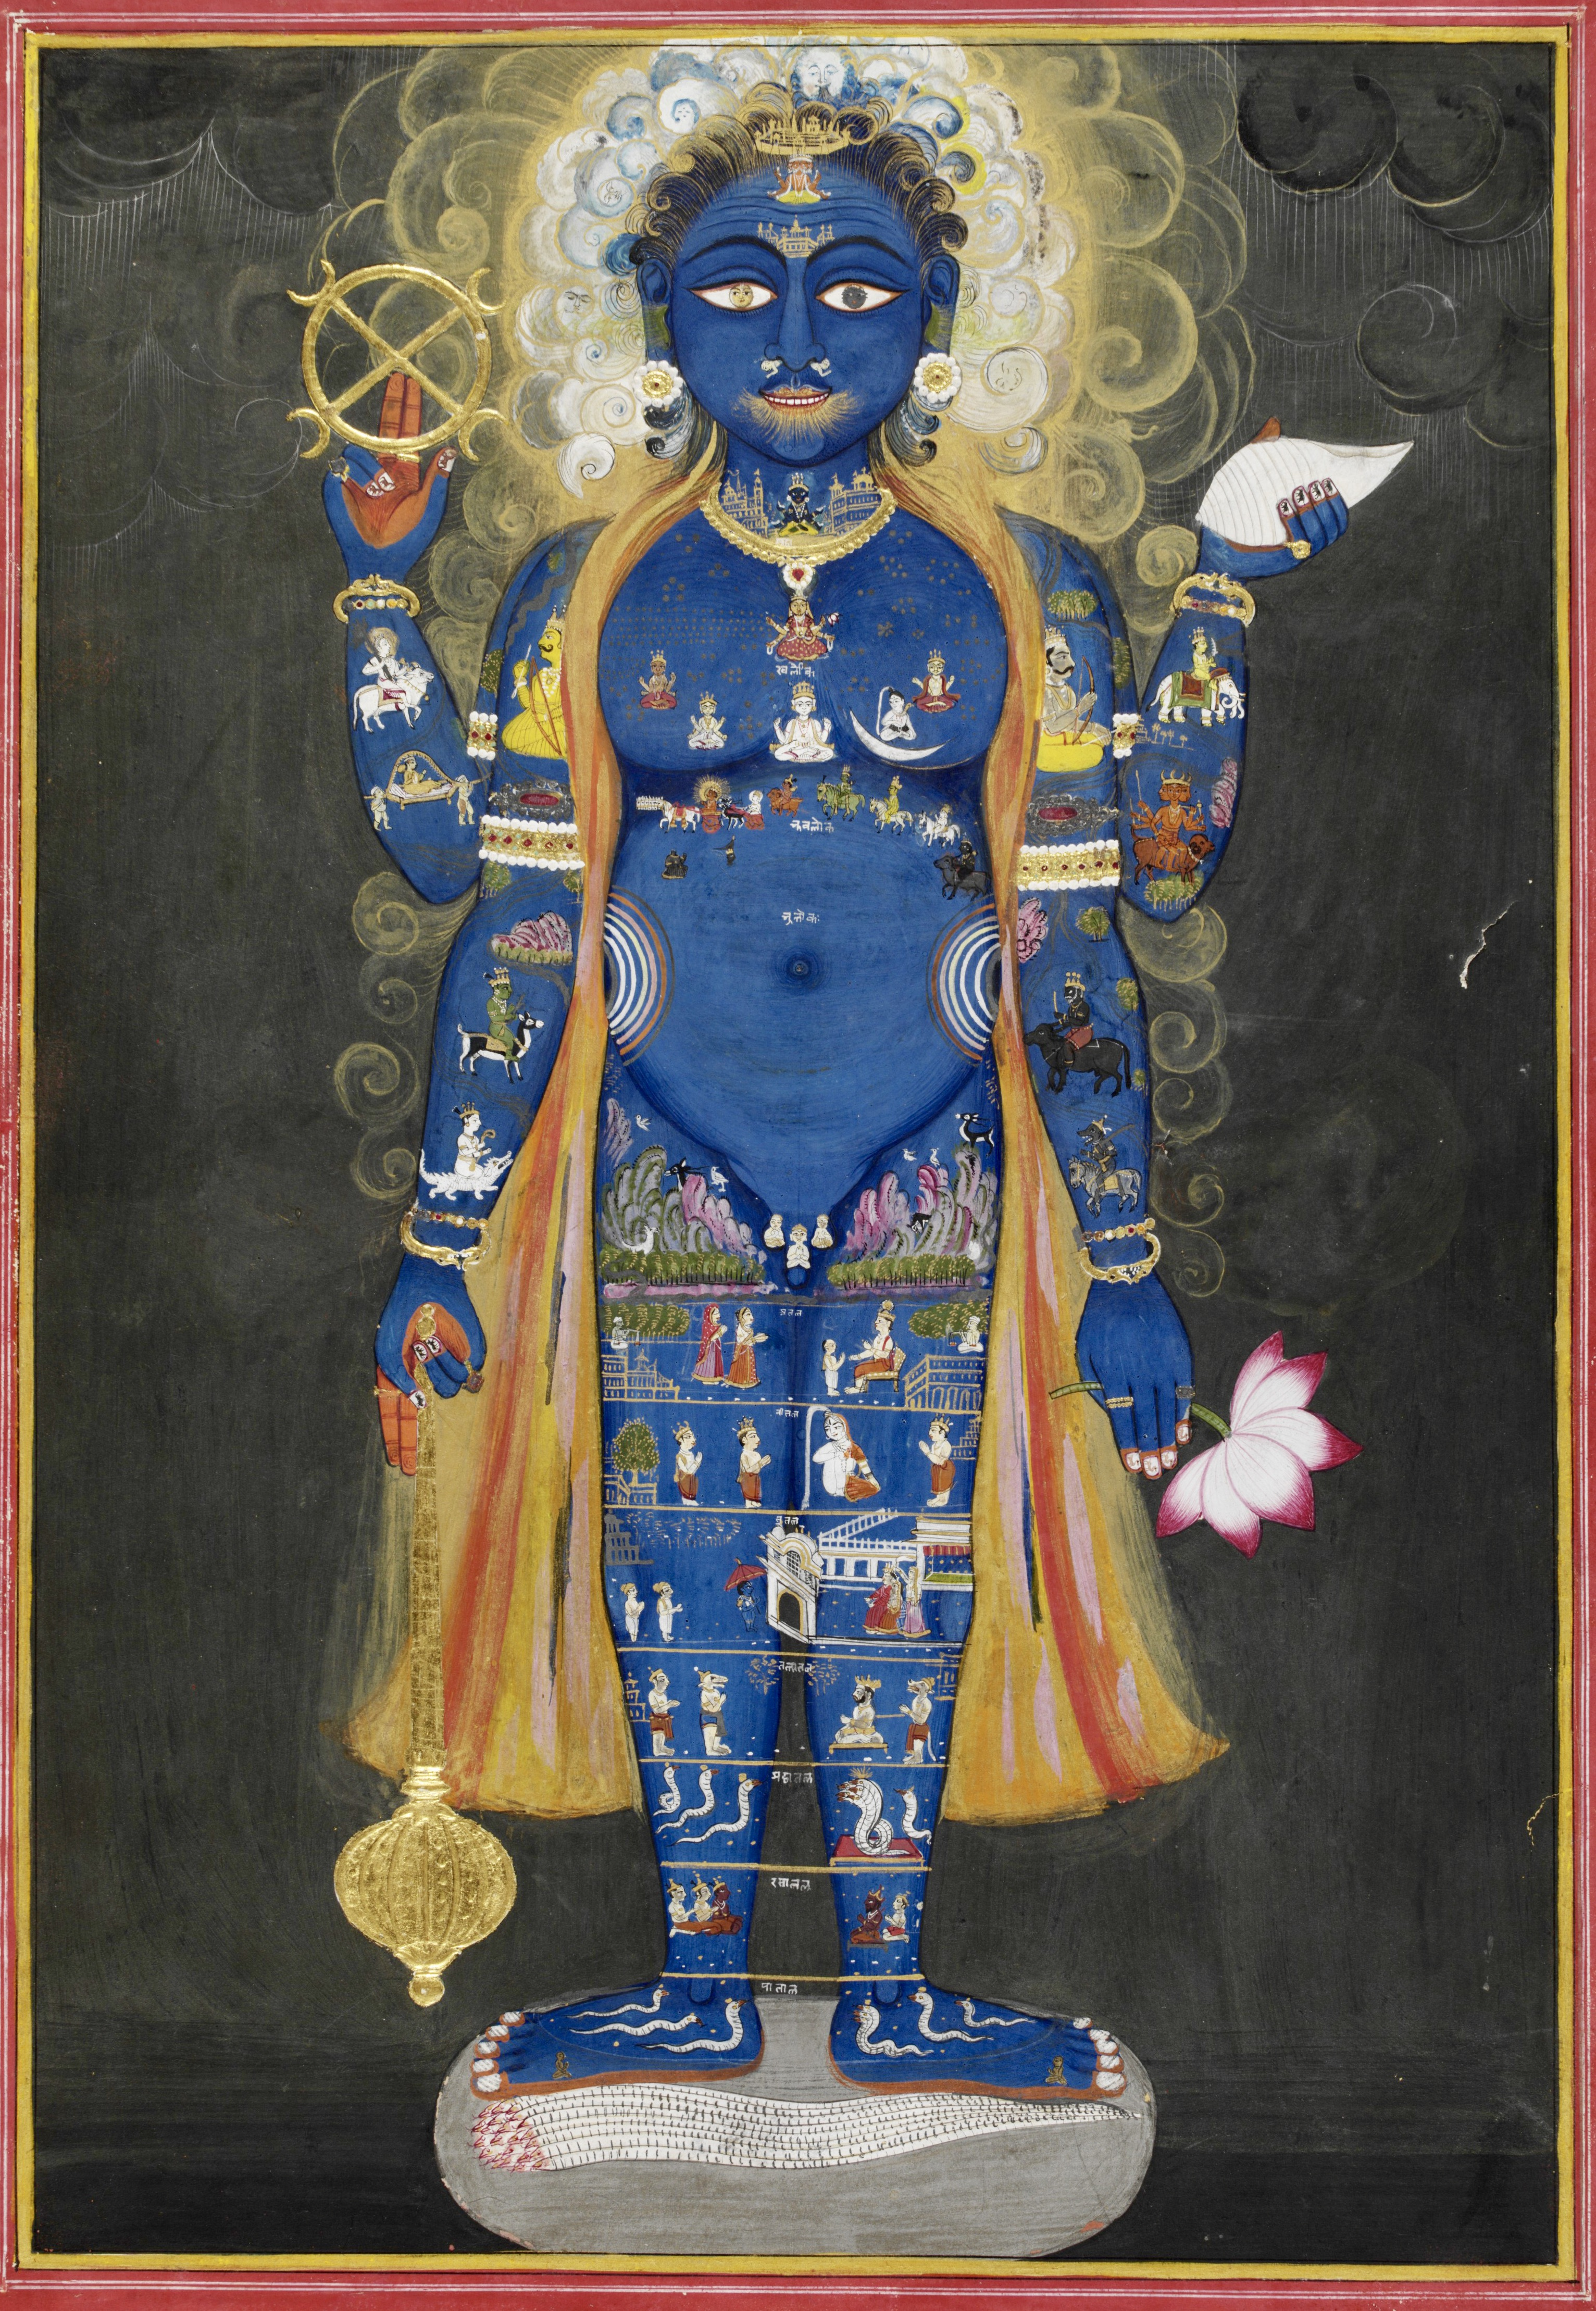
\includegraphics[width=1\textwidth]{pics/Vishnu_Vishvarupa_cropped.jpg}
	\caption{Viṣṇu Viśvarūpa, India, Rajasthan, Jaipur, ca. 1800–1820, Opaque watercolor and gold on paper, 38.5 × 28 cm, Victoria and Albert Museum, London, Given by Mrs. Gerald Clark.}
	\label{fig1}
      \end{figure}
\clearpage
  \begin{figure}[ht]
	\centering
  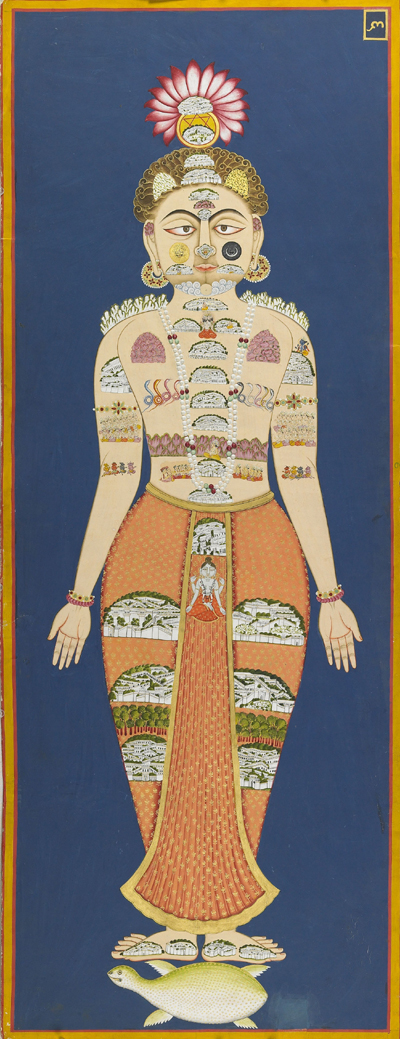
\includegraphics[width=0.5\textwidth]{pics/The_Equivalence_of_Self_and_Universe_(detail),_folio_6_from_the_Siddha_Siddhanta_Paddhati,_(Bulaki),_1824_(Samvat_1881);_122_x_46_cm._Mehrangarh_Museum_Trust..jpg}
	\caption{The Equivalence of Self and Universe (detail), folio 6 from the \textit{Siddhasiddhāntapaddhati} (Bulaki), India, Rajasthan, Jodhpur, 1824 (Samvat 1881), 122 x 46 cm, RJS 2378, Mehragarh Museum Trust.}
	\label{fig2}
      \end{figure}
      % \end{landscape}


\chapter{Bibliography}
 \label{sec:bibli}
   \clearpage
\newpage 
\thispagestyle{empty}
\quad  \addtocounter{page}{-1}

\printbibliography[heading=subbibintoc, title=Consulted Manuscripts, keyword=codex]

\printbibliography[heading=subbibintoc, title=Printed Editions, keyword=printsource]

\printbibliography[heading=subbibintoc, title=Secondary Literature, keyword=seclit]

\printbibliography[heading=subbibintoc, title=Online Sources, keyword=onlinesource]

\end{document}
